\chapter{Supplementary Convergence and Target-Precision Profiles}
\label{app:benchmark_profiles}

This appendix completes the profile grid illustrated in
Chapter~\ref{chap:experiments}: all three LLMs are represented at
$D=2$ and $D=5$. Explicit profiles use $\sigma=0$, $0.05$, and $0.2$;
Implicit profiles use the positive noise levels $\sigma=0.05$ and $0.2$.
The six pairs already shown in the main chapter are not repeated here.
Together, the chapter and appendix provide all 30 condition-specific
pairs. The intermediate level $\sigma=0.1$ remains part of the
experimental protocol and quantitative summaries; its profiles are
omitted only to limit the illustrated grid.

Each pair shows convergence above and adaptive target-precision ECDF
below, with separate panels for $f_1$, $f_8$, $f_{11}$, $f_{15}$, and
$f_{21}$. Convergence summarizes queried clean optimality gaps using
the median and interquartile range. The ECDF summarizes attainment
over trial--target pairs, not returned-solution success at one fixed
threshold. The panel legends identify generated prompt strategies and
classical baselines. Comparisons should use matching functions,
dimensions, synthesis modes, and noise levels; adaptive target sets
must also be considered when interpreting ECDF magnitudes.

The objective-query allowance is $10{,}000D$: 20,000 queries in two
dimensions and 50,000 in five dimensions. Displayed trajectories may
extend beyond a run's last query through carry-forward; this does not
indicate additional evaluations.

% Keep profile pairs in document order rather than on separate float pages.
% Compact height leaves room for section/model headings and the caption.
\section{Explicit Profiles}
\nopagebreak[4]

\subsection{Qwen2.5-Coder-14B-Instruct}
\nopagebreak[4]

\par\smallskip\noindent
\begin{minipage}{\linewidth}
    \captionsetup{type=figure,aboveskip=4pt,belowskip=0pt}
    \centering
    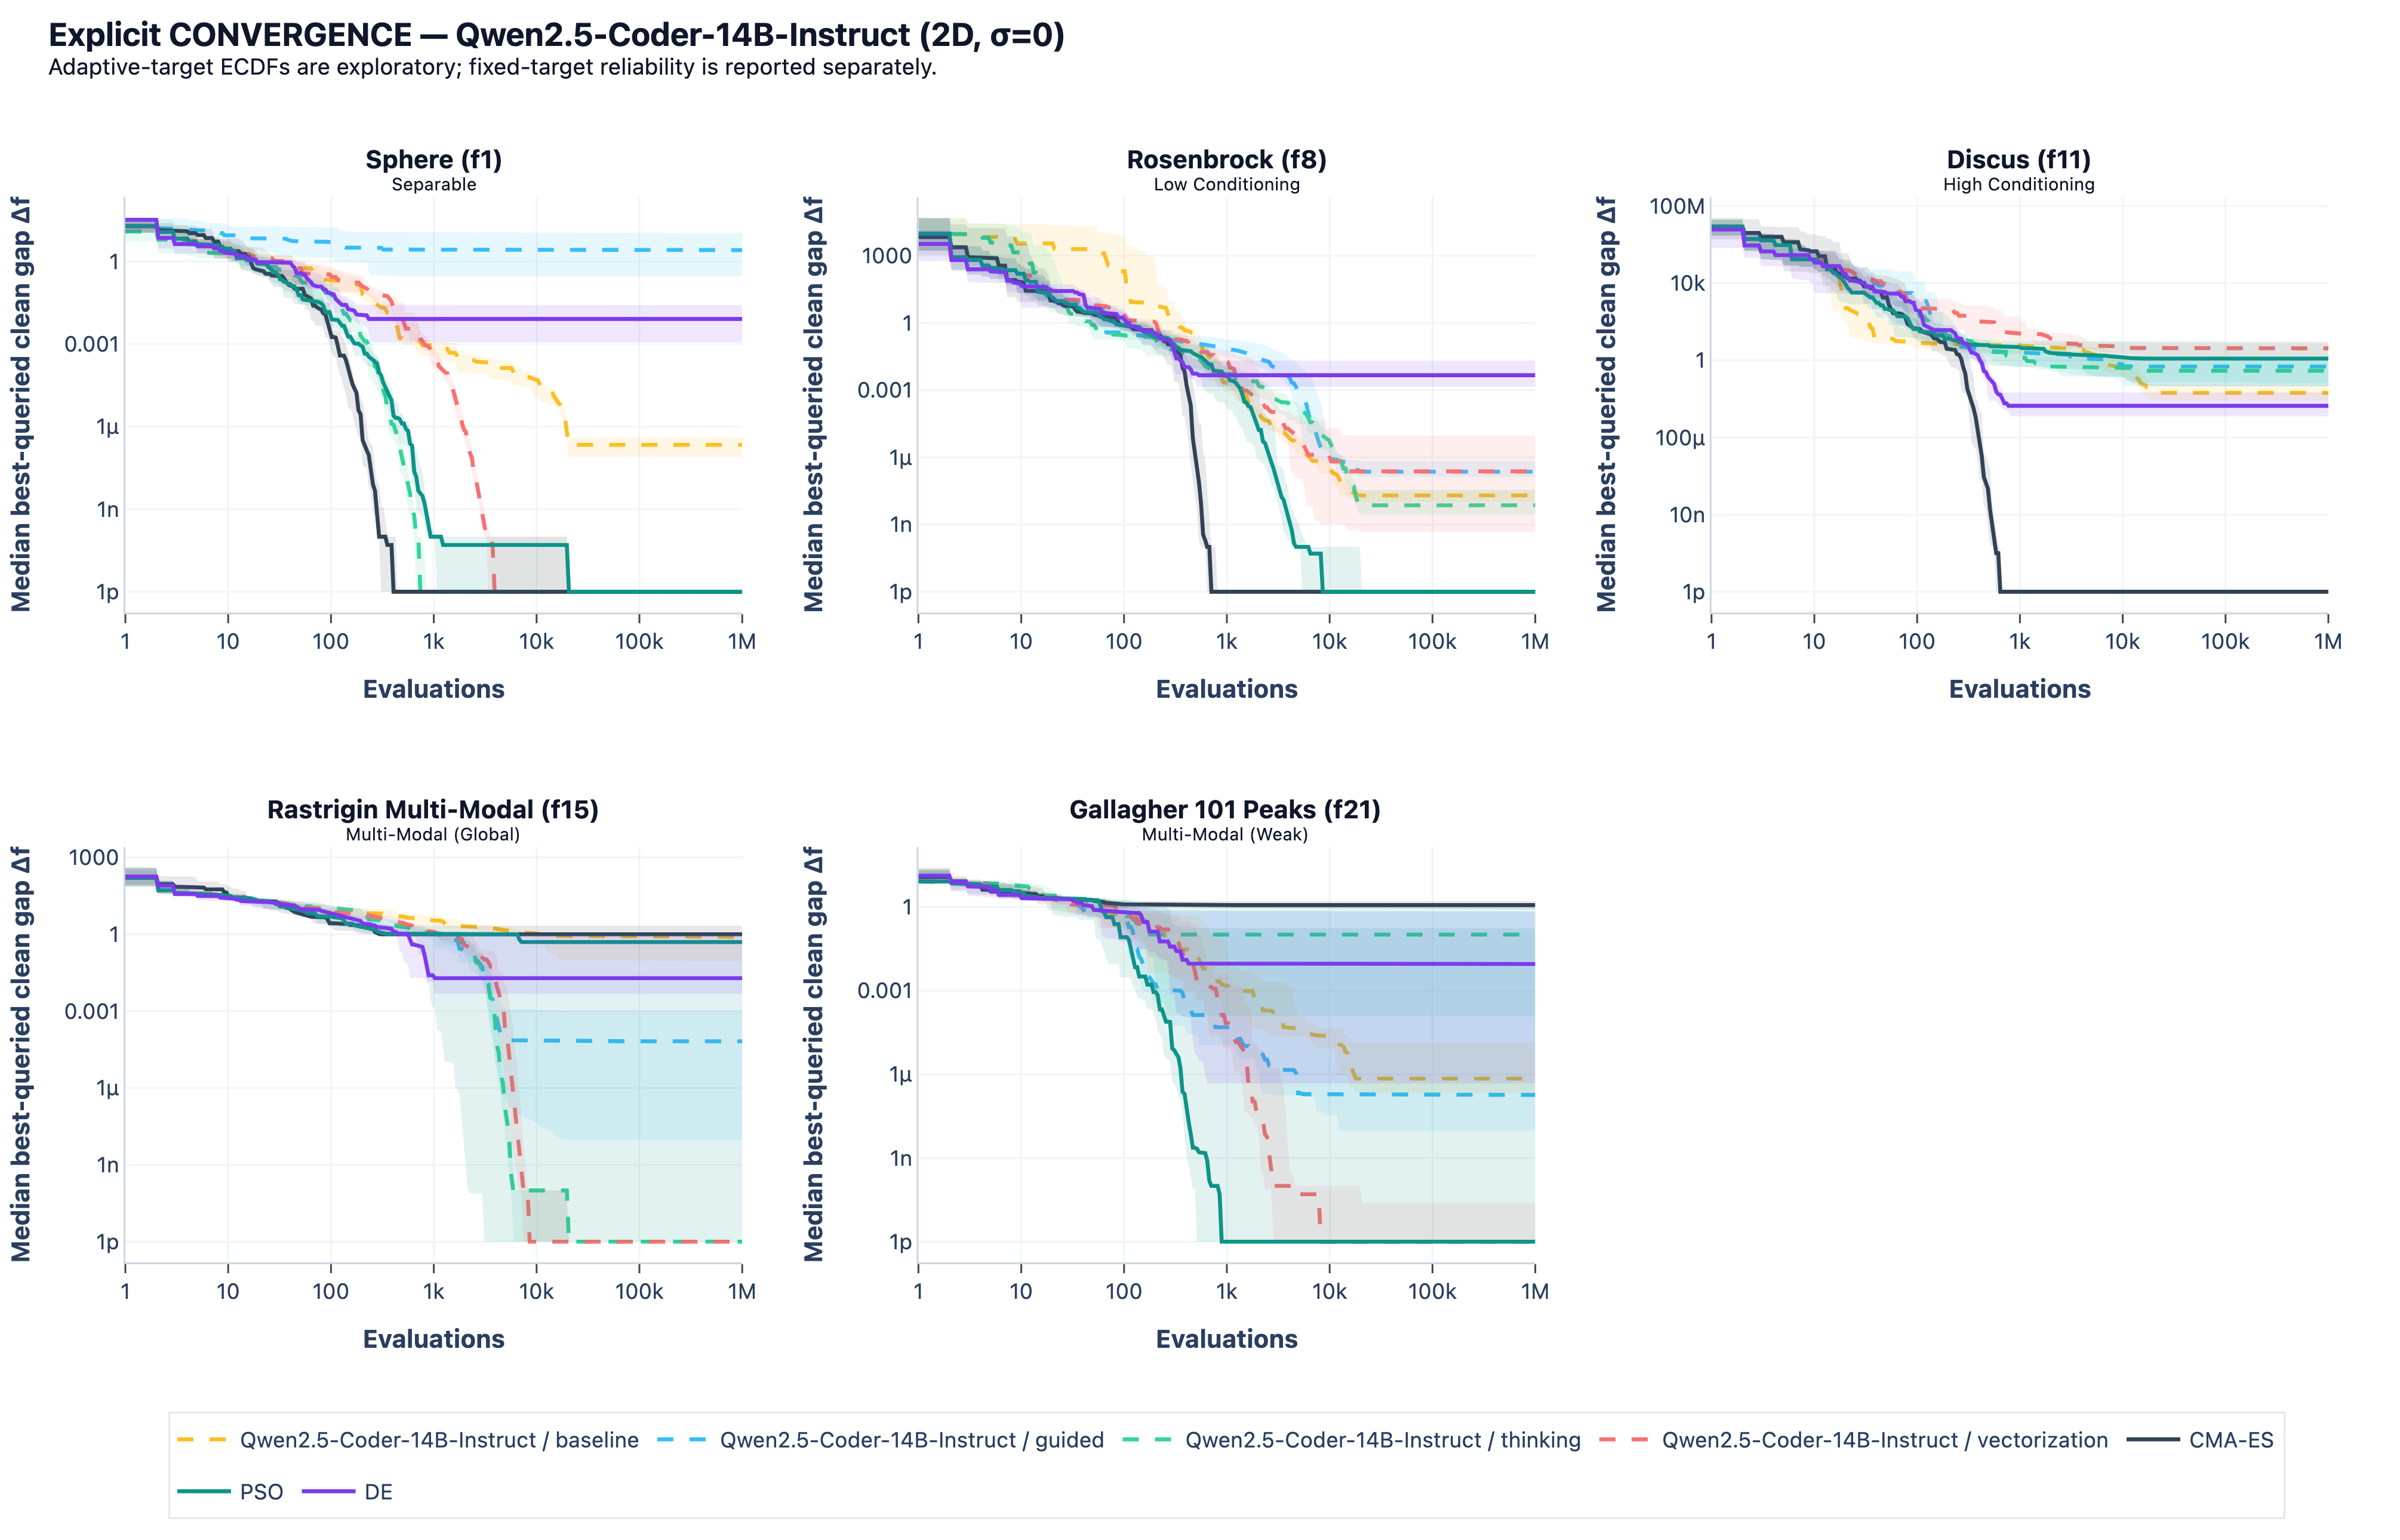
\includegraphics[width=\textwidth,height=0.32\textheight,keepaspectratio]{images/experiments/02_explicit/qwen_14b/2D/std_0.0/convergence_trajectories.png}
    \par\medskip
    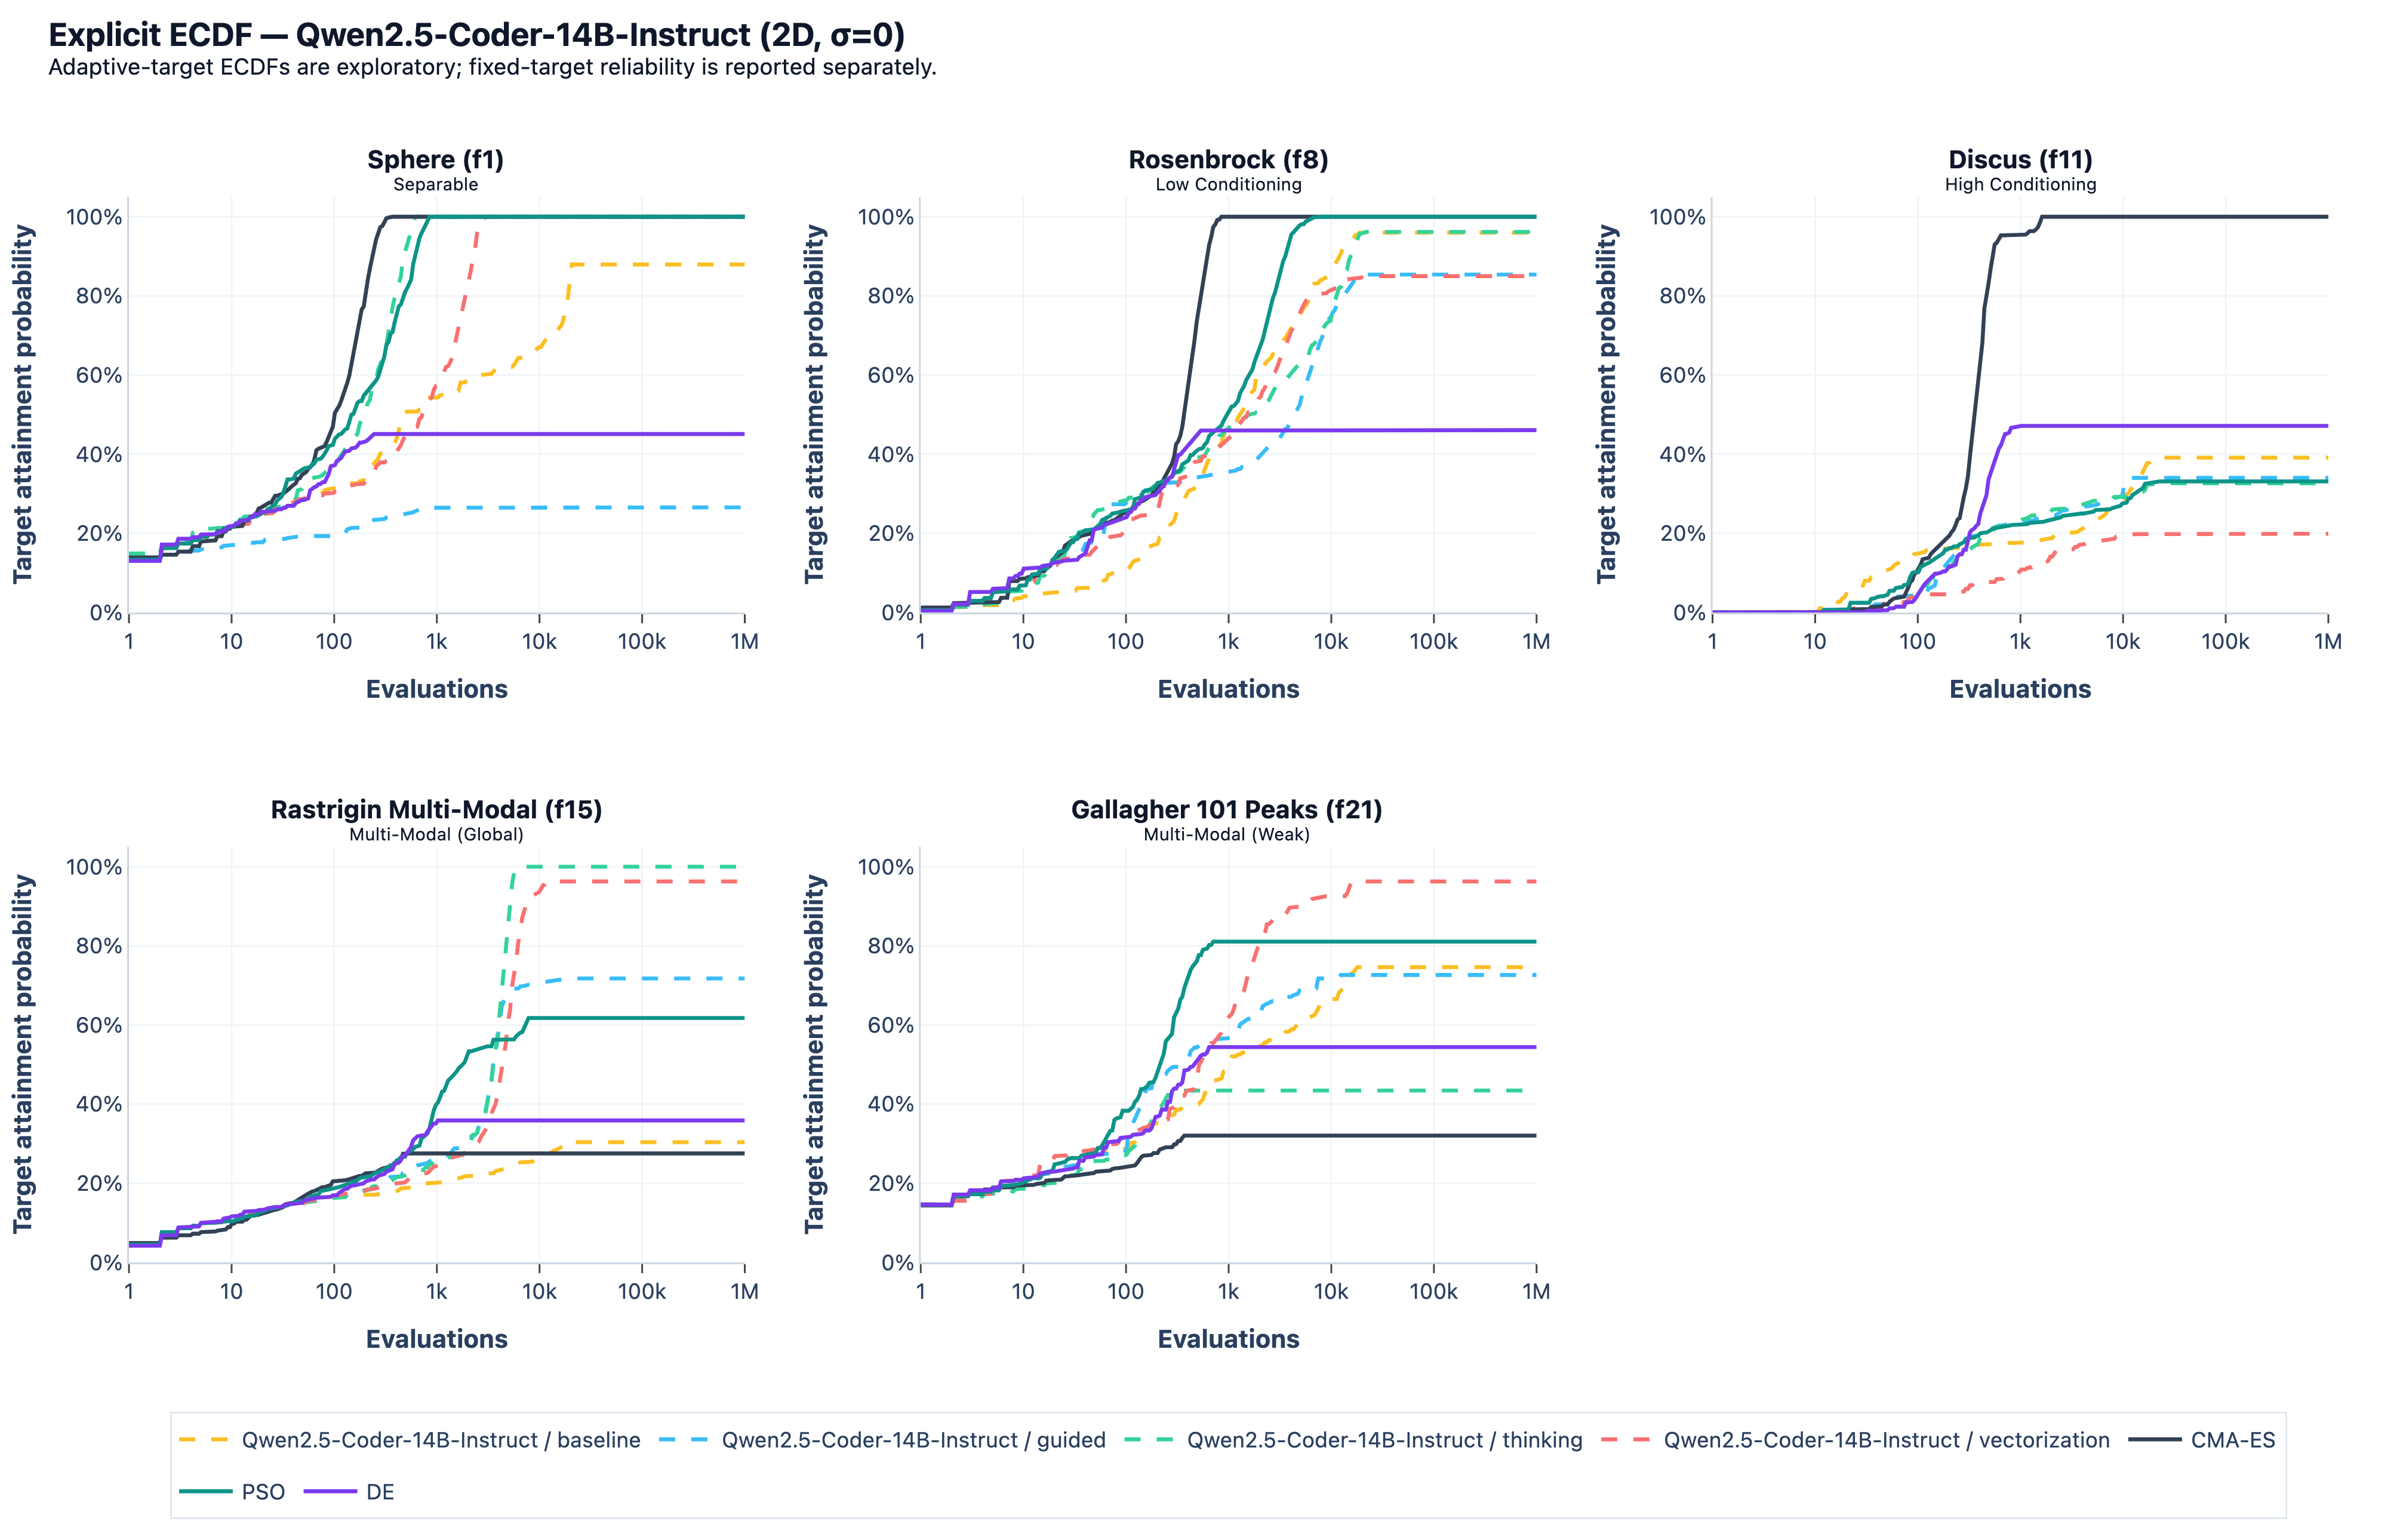
\includegraphics[width=\textwidth,height=0.32\textheight,keepaspectratio]{images/experiments/02_explicit/qwen_14b/2D/std_0.0/target_precision_ecdf.png}
    \caption{Qwen2.5-Coder-14B-Instruct: Explicit, $D=2$,
    $\sigma=0.0$. Convergence (median and IQR) above;
    adaptive target-precision ECDF below. The objective-query allowance
    is 20,000.}
    \label{fig:appendix_02_explicit_qwen_14b_2_std_00}
\end{minipage}
\par\medskip

\par\smallskip\noindent
\begin{minipage}{\linewidth}
    \captionsetup{type=figure,aboveskip=4pt,belowskip=0pt}
    \centering
    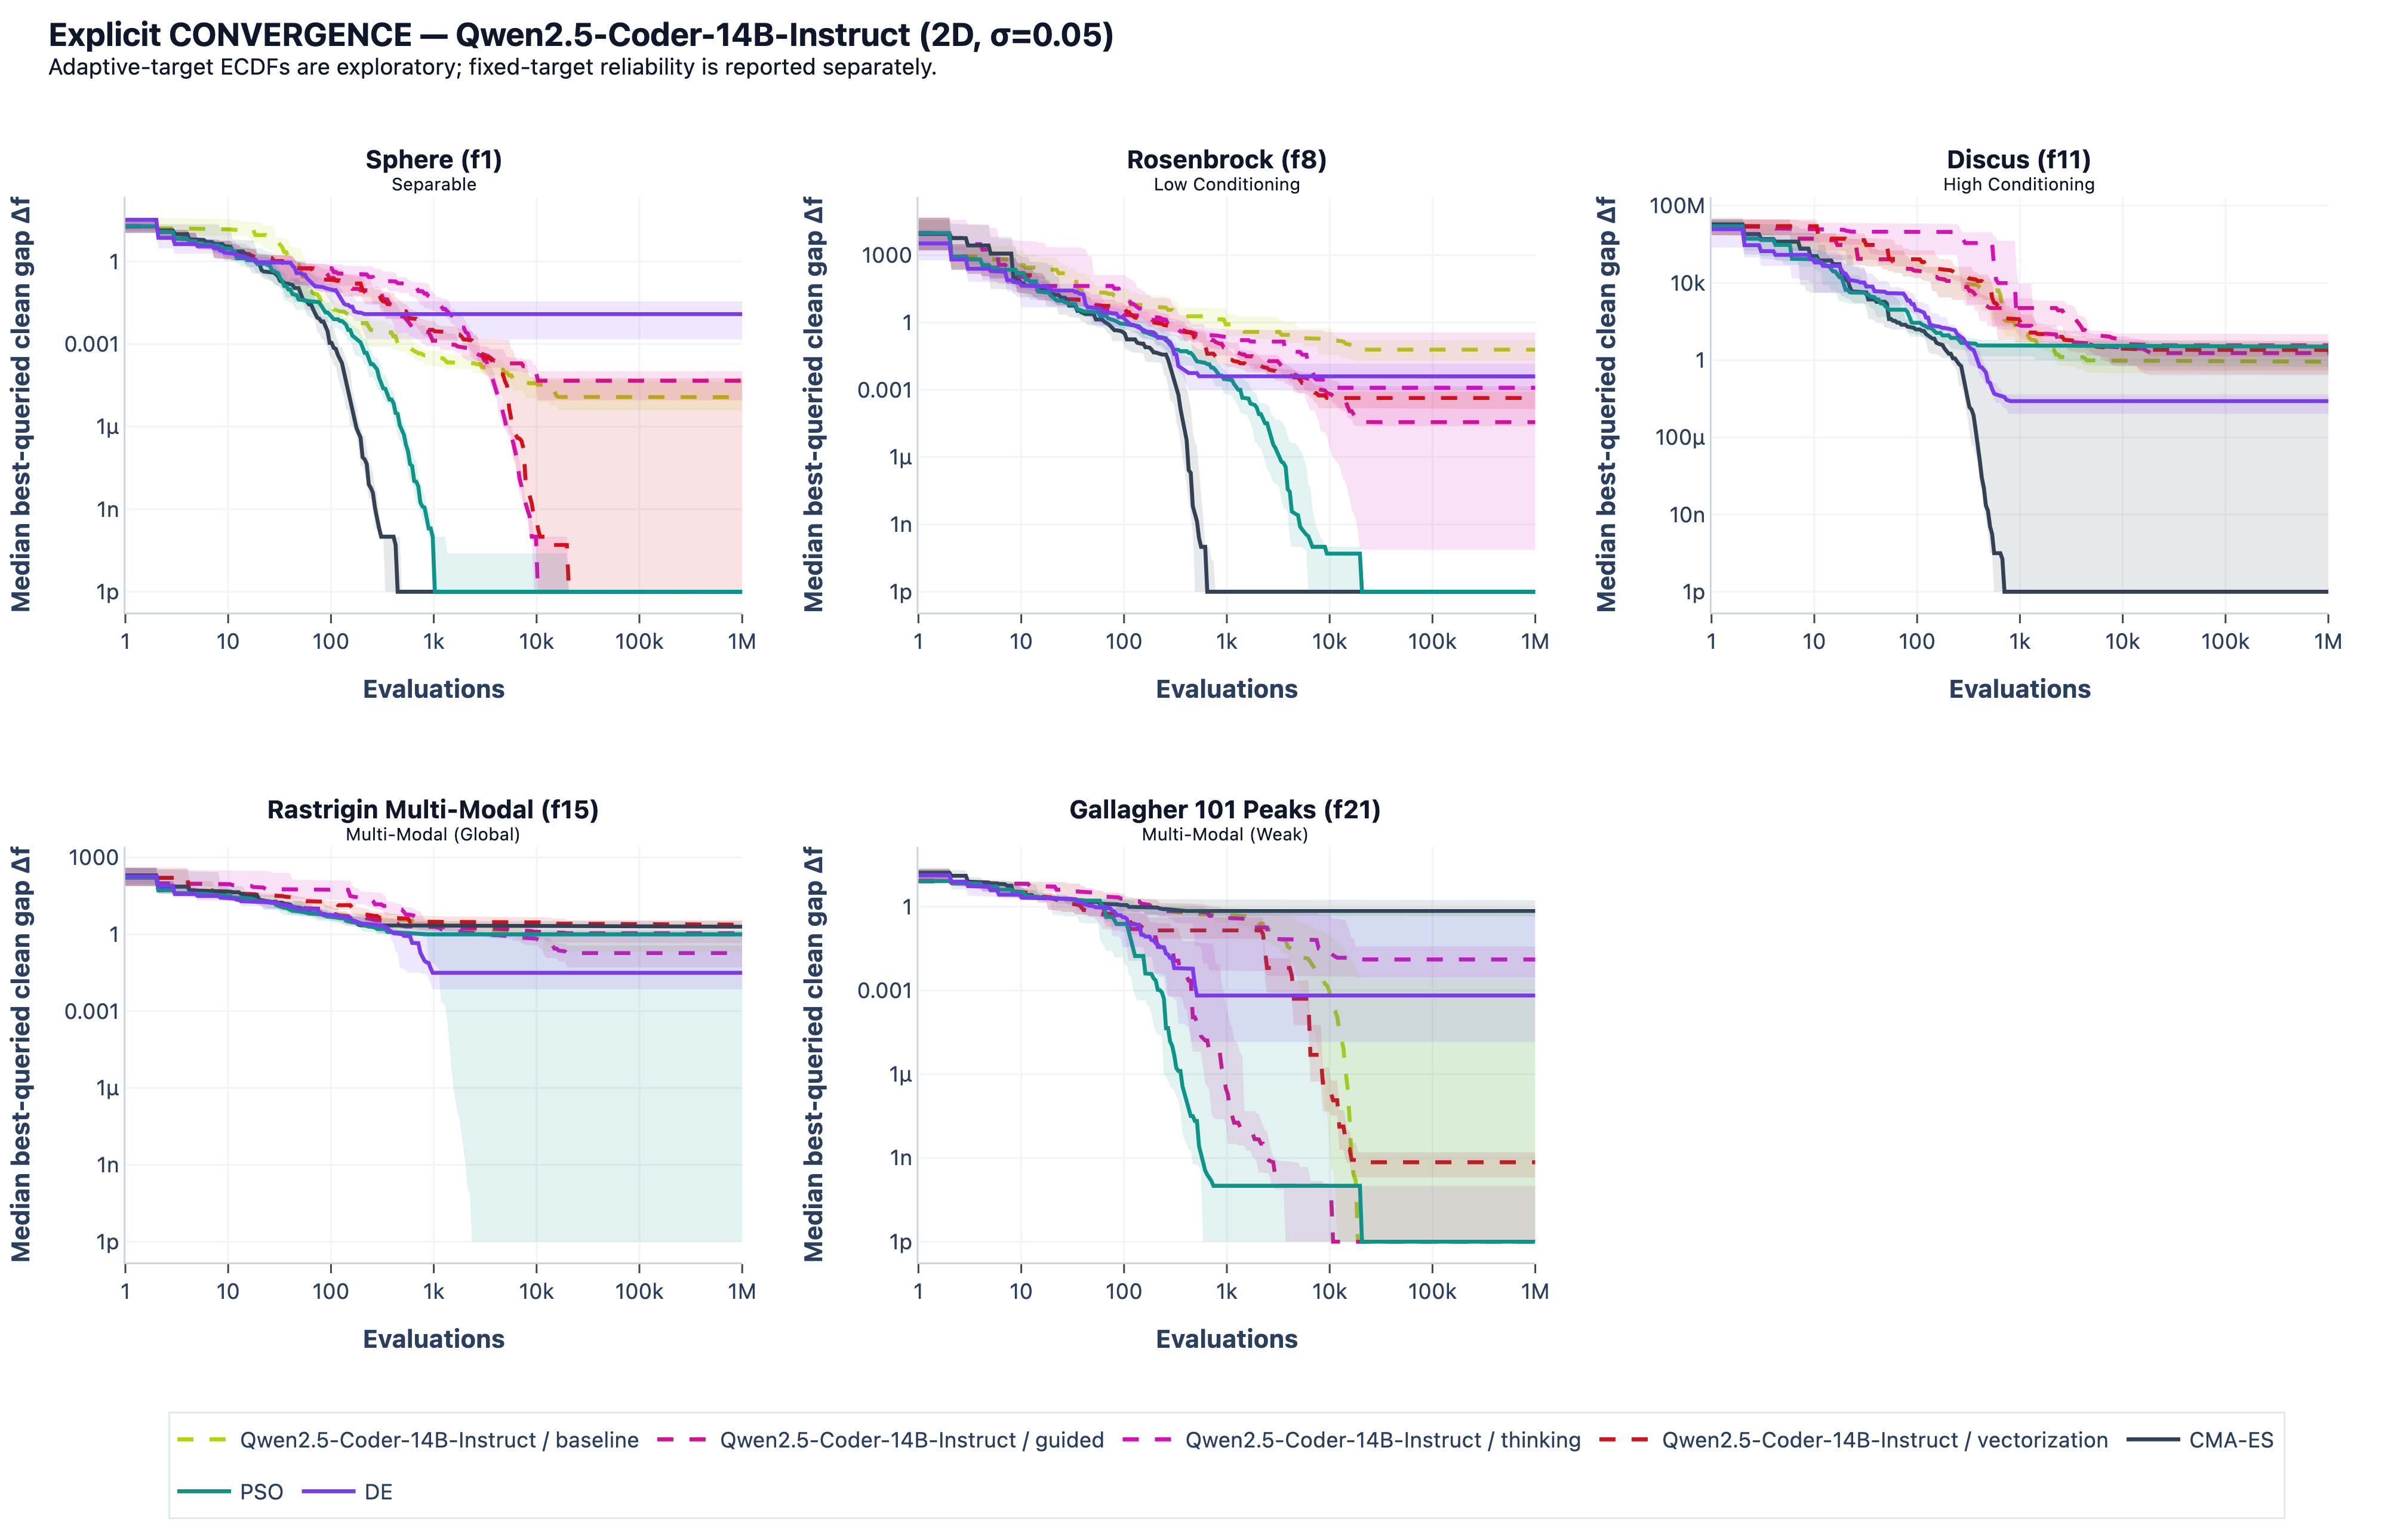
\includegraphics[width=\textwidth,height=0.32\textheight,keepaspectratio]{images/experiments/02_explicit/qwen_14b/2D/std_0.05/convergence_trajectories.png}
    \par\medskip
    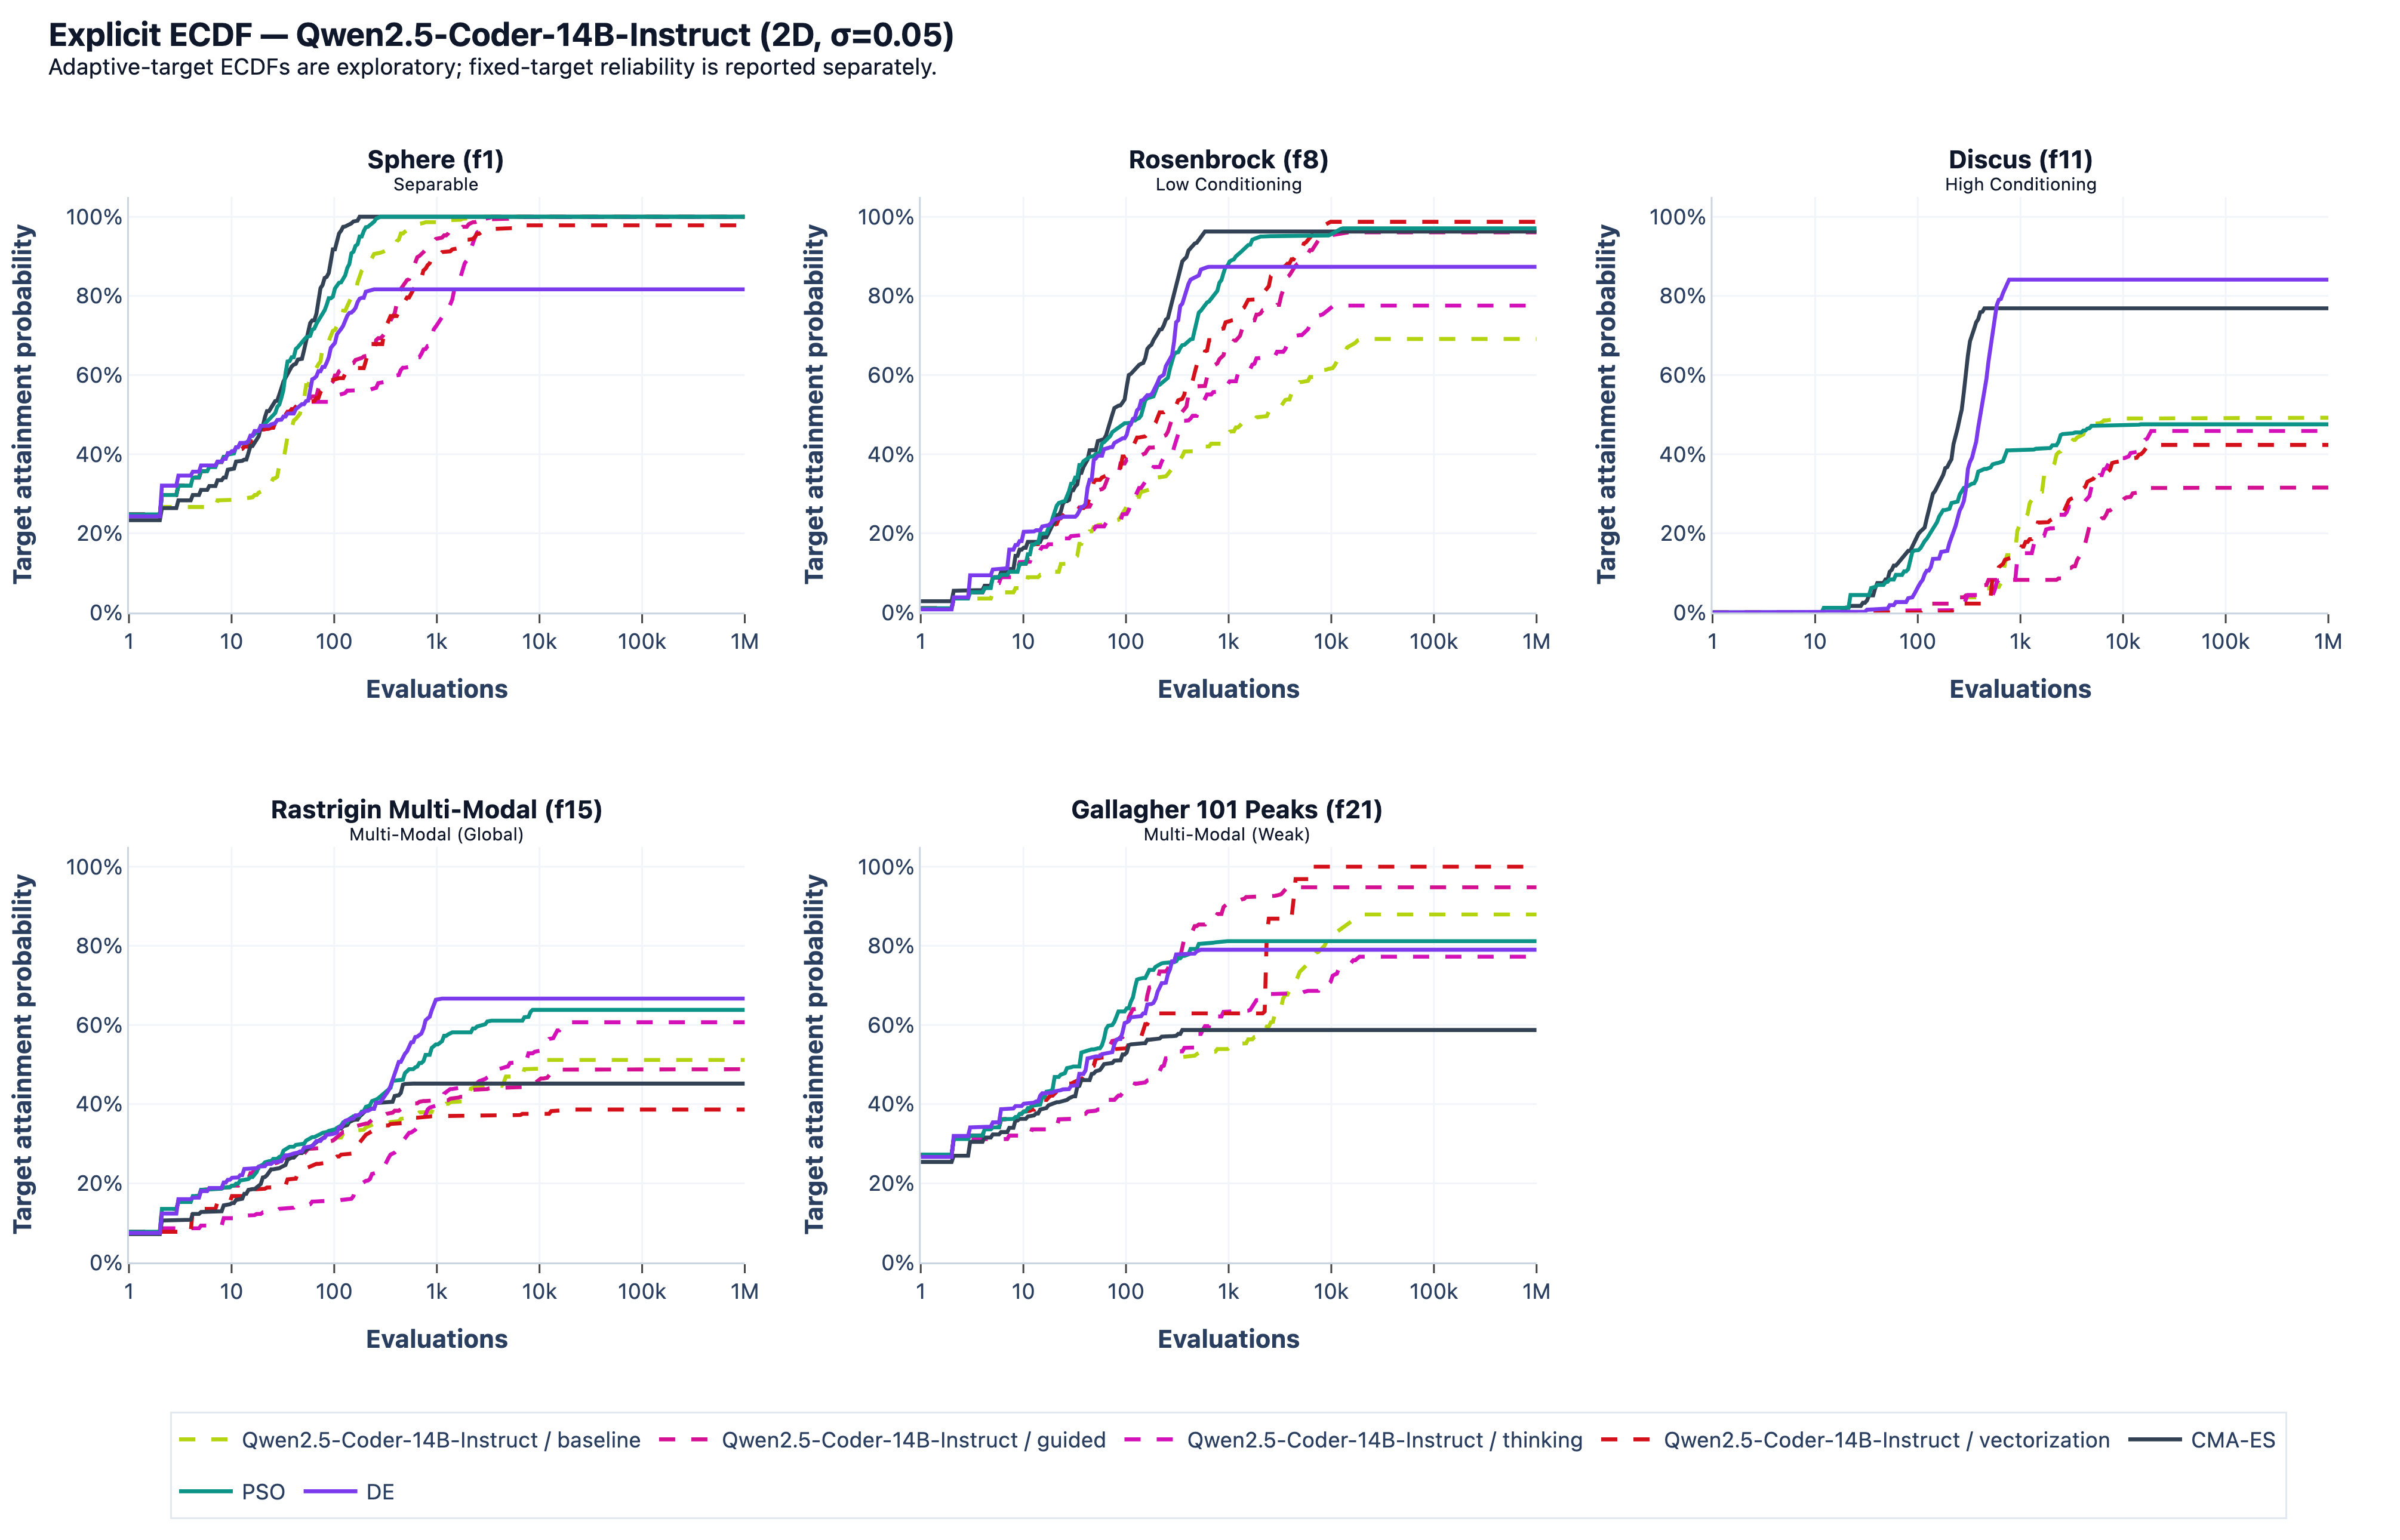
\includegraphics[width=\textwidth,height=0.32\textheight,keepaspectratio]{images/experiments/02_explicit/qwen_14b/2D/std_0.05/target_precision_ecdf.png}
    \caption{Qwen2.5-Coder-14B-Instruct: Explicit, $D=2$,
    $\sigma=0.05$. Convergence (median and IQR) above;
    adaptive target-precision ECDF below. The objective-query allowance
    is 20,000.}
    \label{fig:appendix_02_explicit_qwen_14b_2_std_005}
\end{minipage}
\par\medskip

\par\smallskip\noindent
\begin{minipage}{\linewidth}
    \captionsetup{type=figure,aboveskip=4pt,belowskip=0pt}
    \centering
    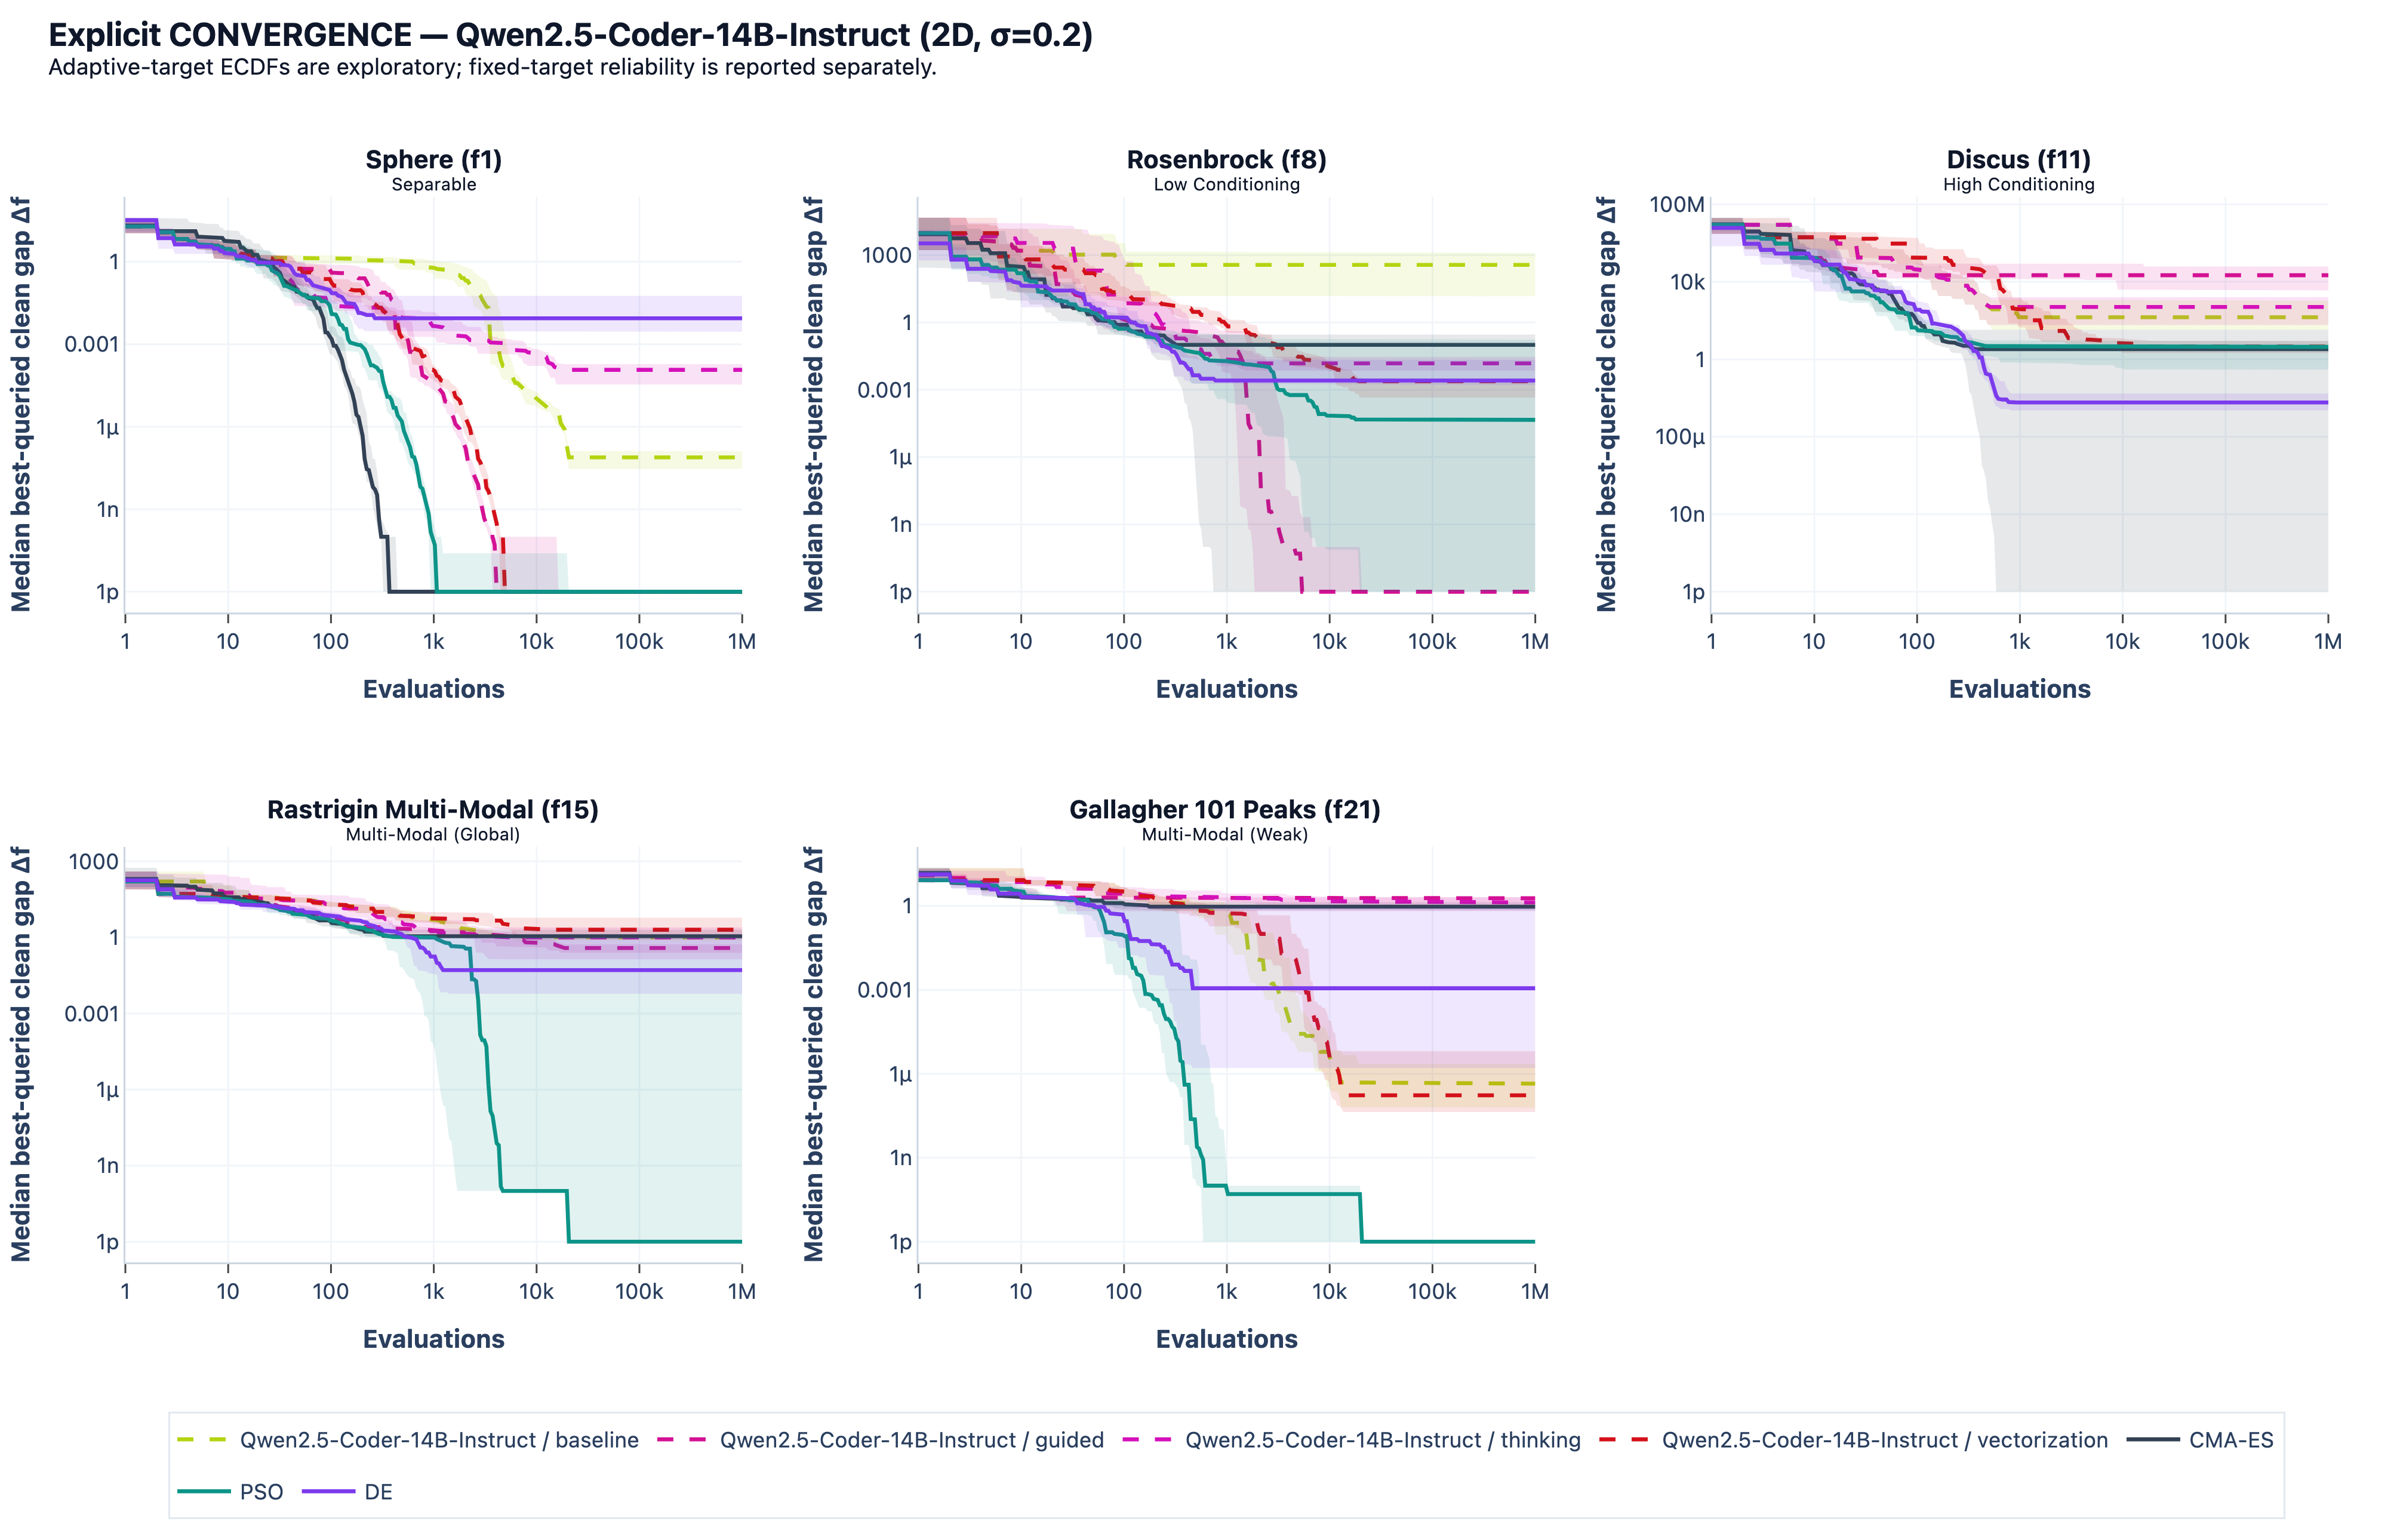
\includegraphics[width=\textwidth,height=0.32\textheight,keepaspectratio]{images/experiments/02_explicit/qwen_14b/2D/std_0.2/convergence_trajectories.png}
    \par\medskip
    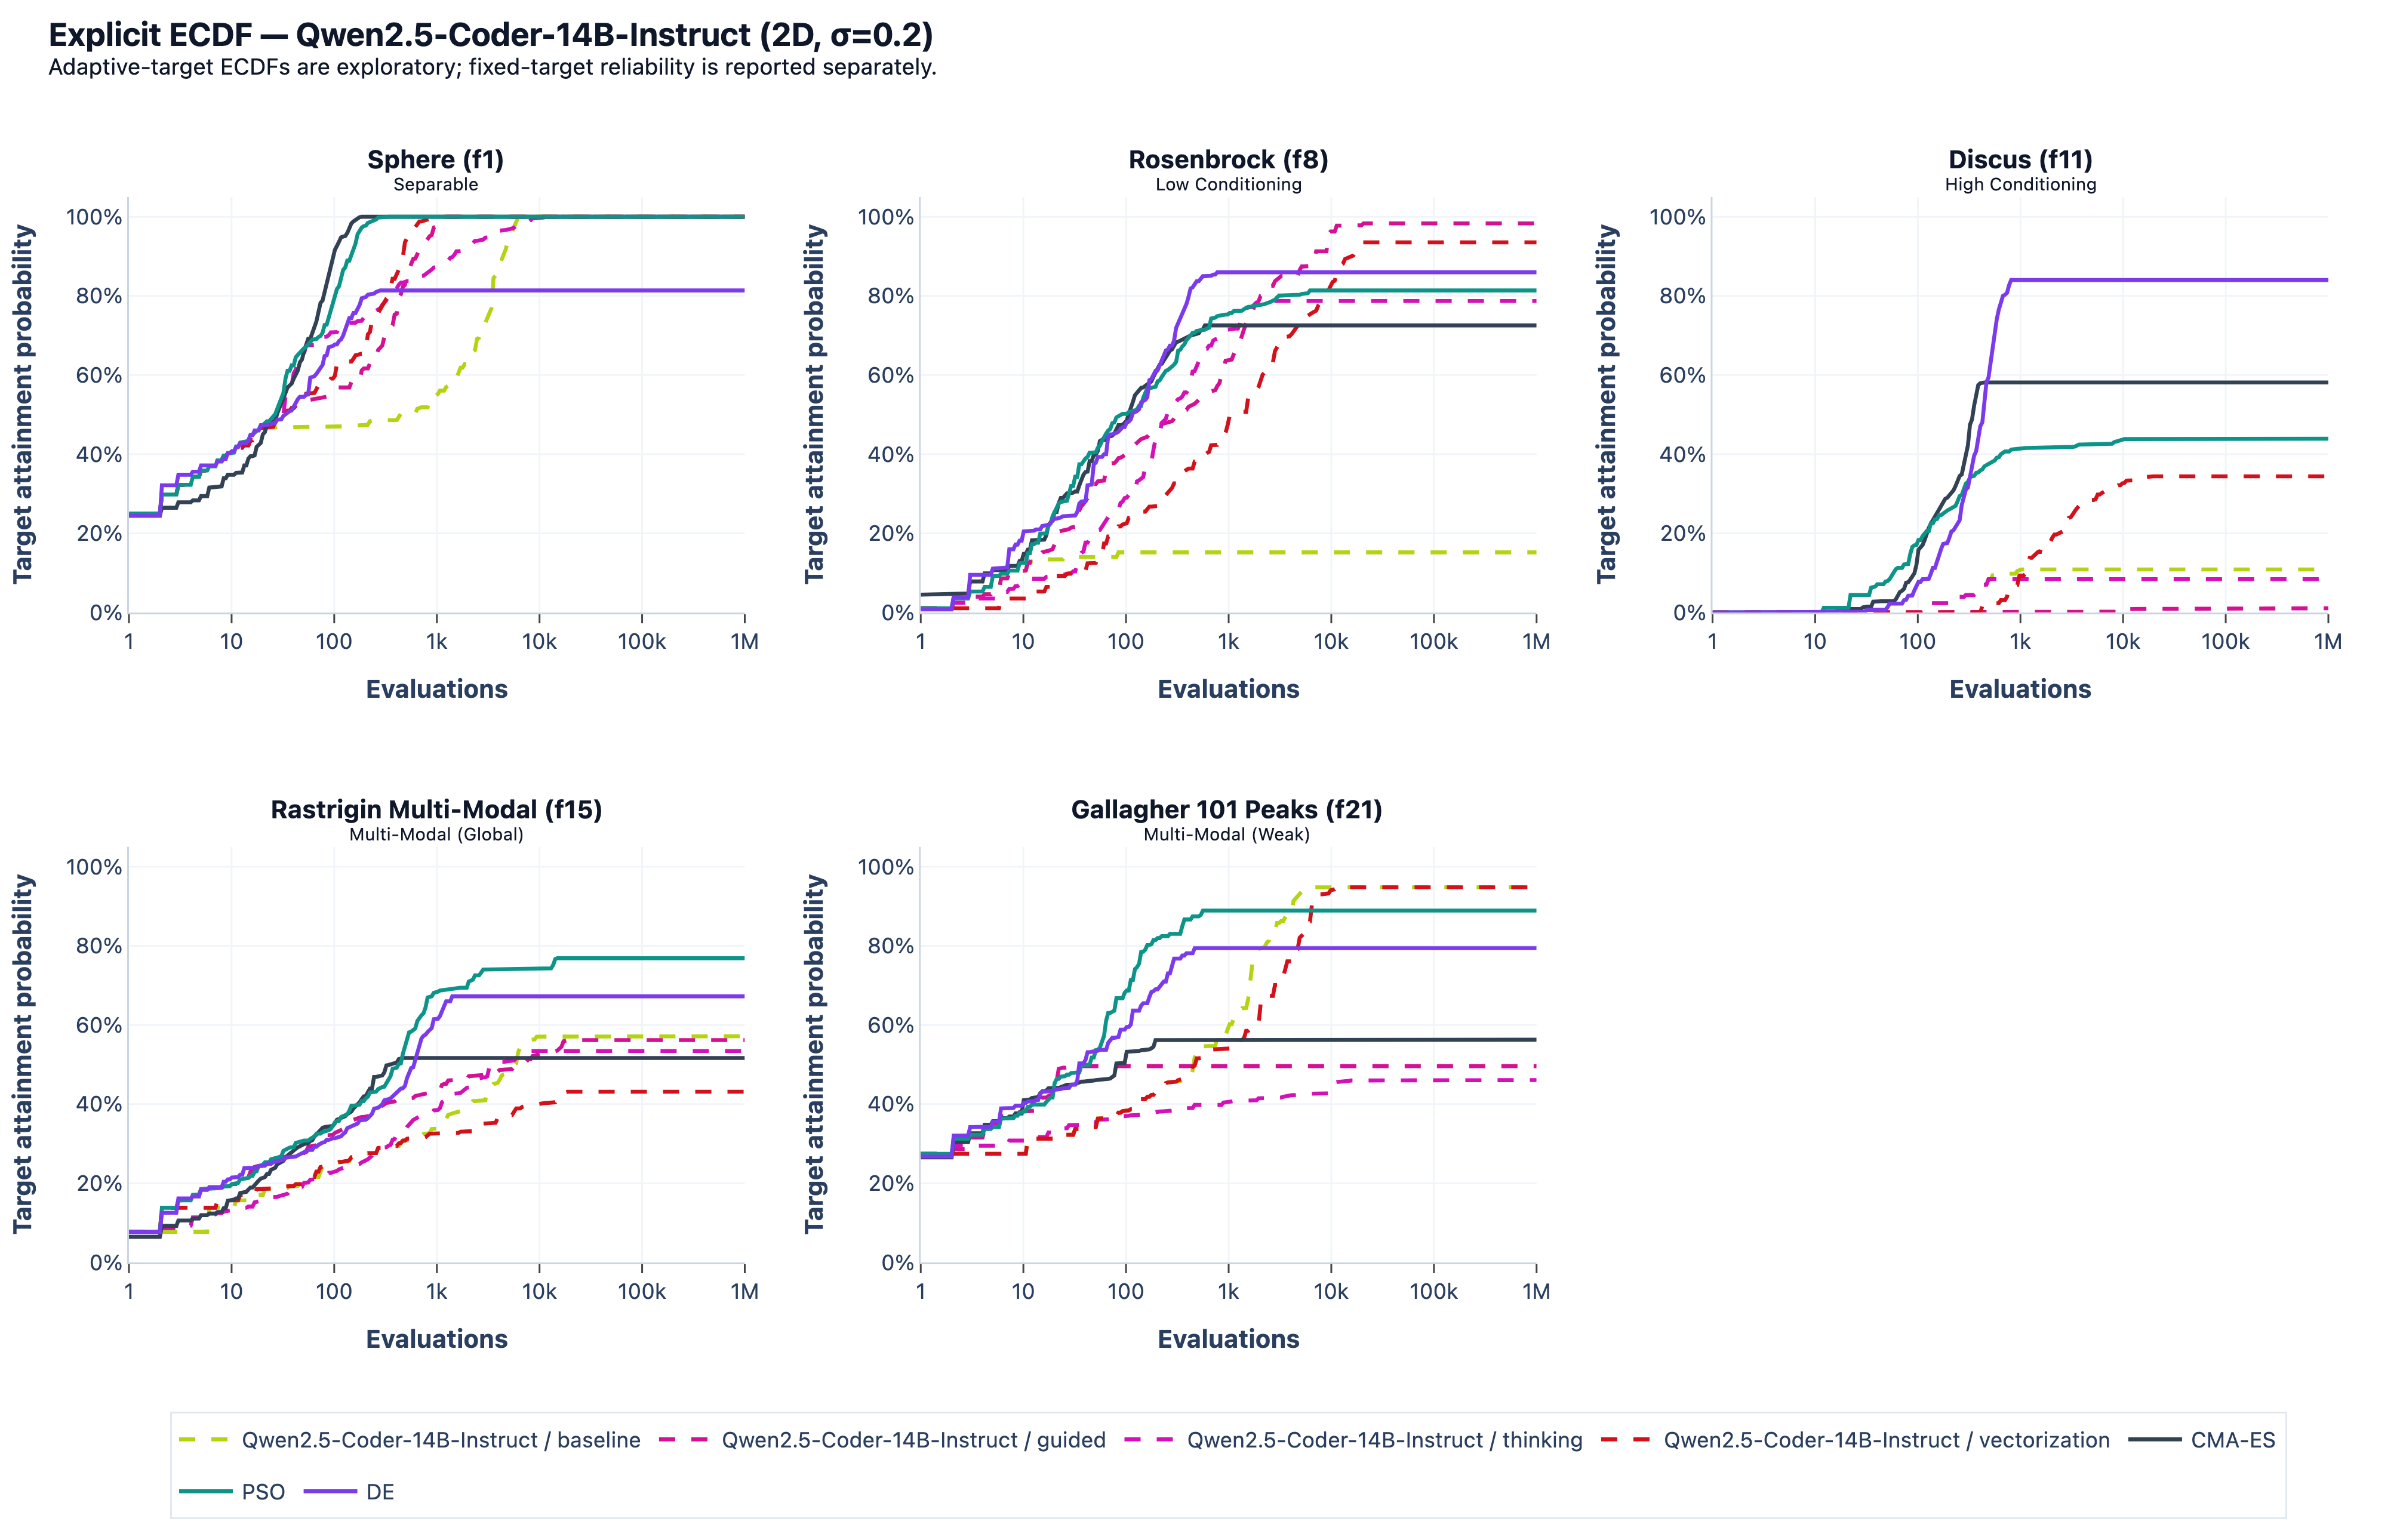
\includegraphics[width=\textwidth,height=0.32\textheight,keepaspectratio]{images/experiments/02_explicit/qwen_14b/2D/std_0.2/target_precision_ecdf.png}
    \caption{Qwen2.5-Coder-14B-Instruct: Explicit, $D=2$,
    $\sigma=0.2$. Convergence (median and IQR) above;
    adaptive target-precision ECDF below. The objective-query allowance
    is 20,000.}
    \label{fig:appendix_02_explicit_qwen_14b_2_std_02}
\end{minipage}
\par\medskip

\par\smallskip\noindent
\begin{minipage}{\linewidth}
    \captionsetup{type=figure,aboveskip=4pt,belowskip=0pt}
    \centering
    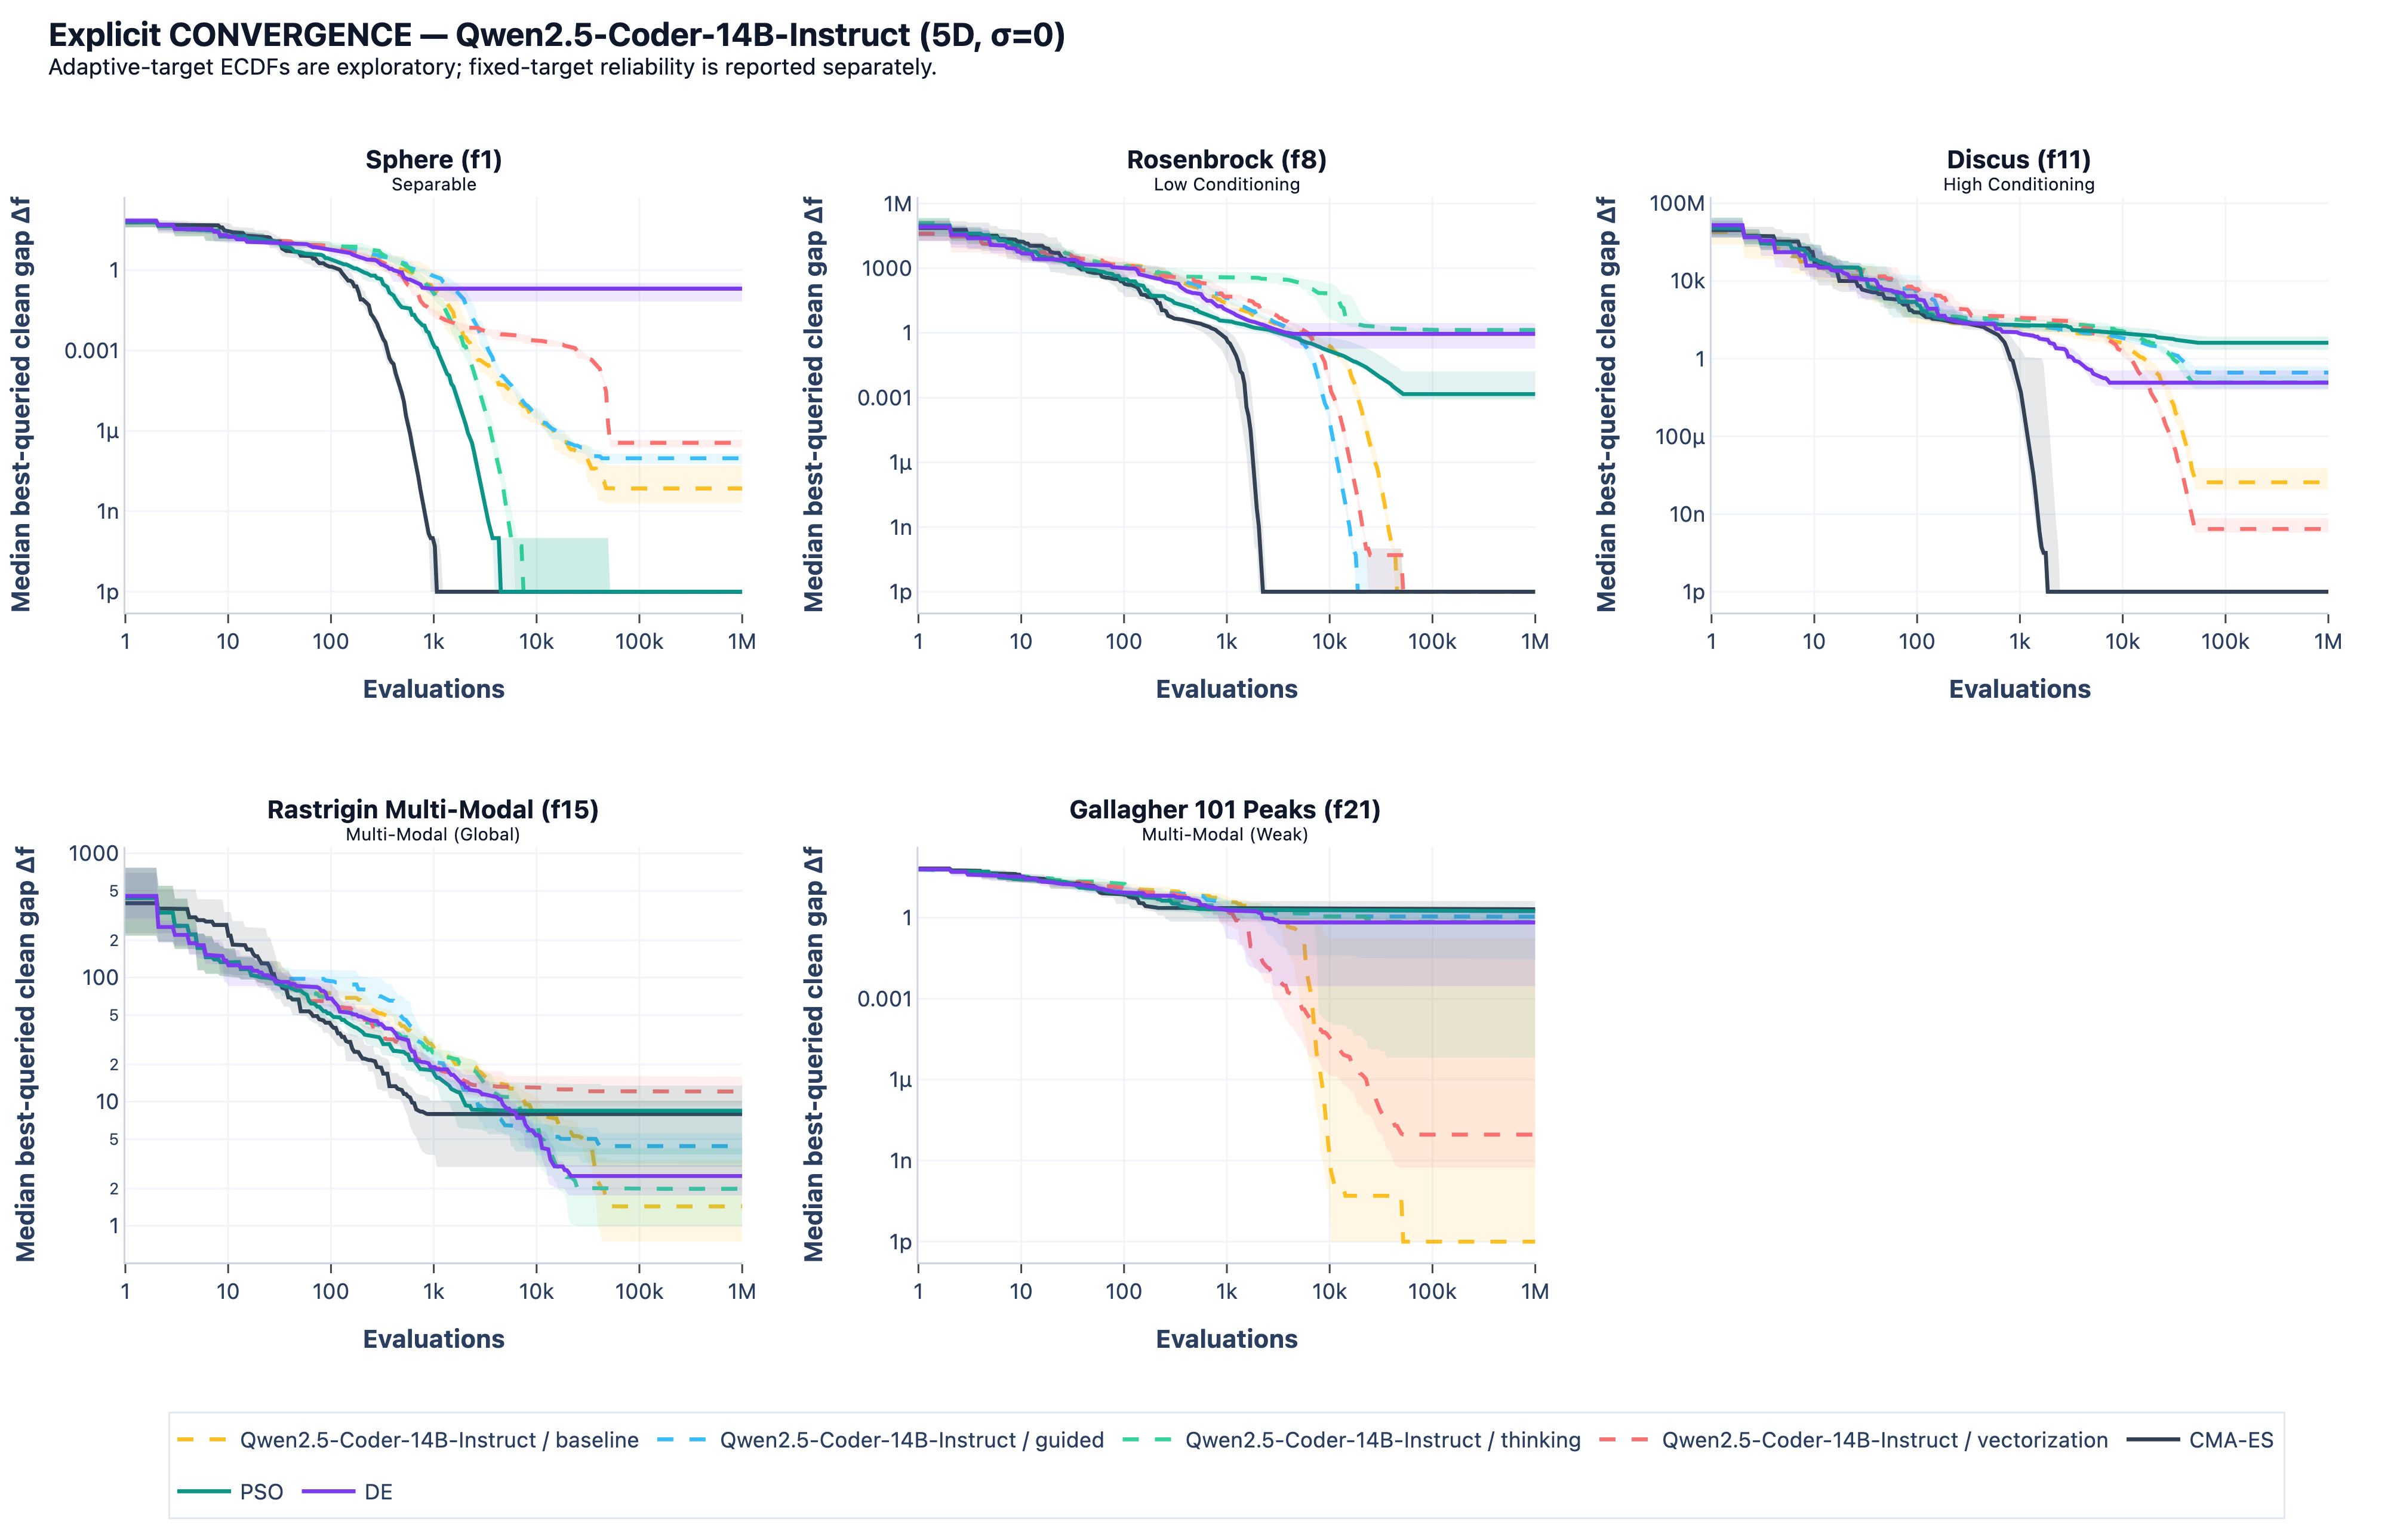
\includegraphics[width=\textwidth,height=0.32\textheight,keepaspectratio]{images/experiments/02_explicit/qwen_14b/5D/std_0.0/convergence_trajectories.png}
    \par\medskip
    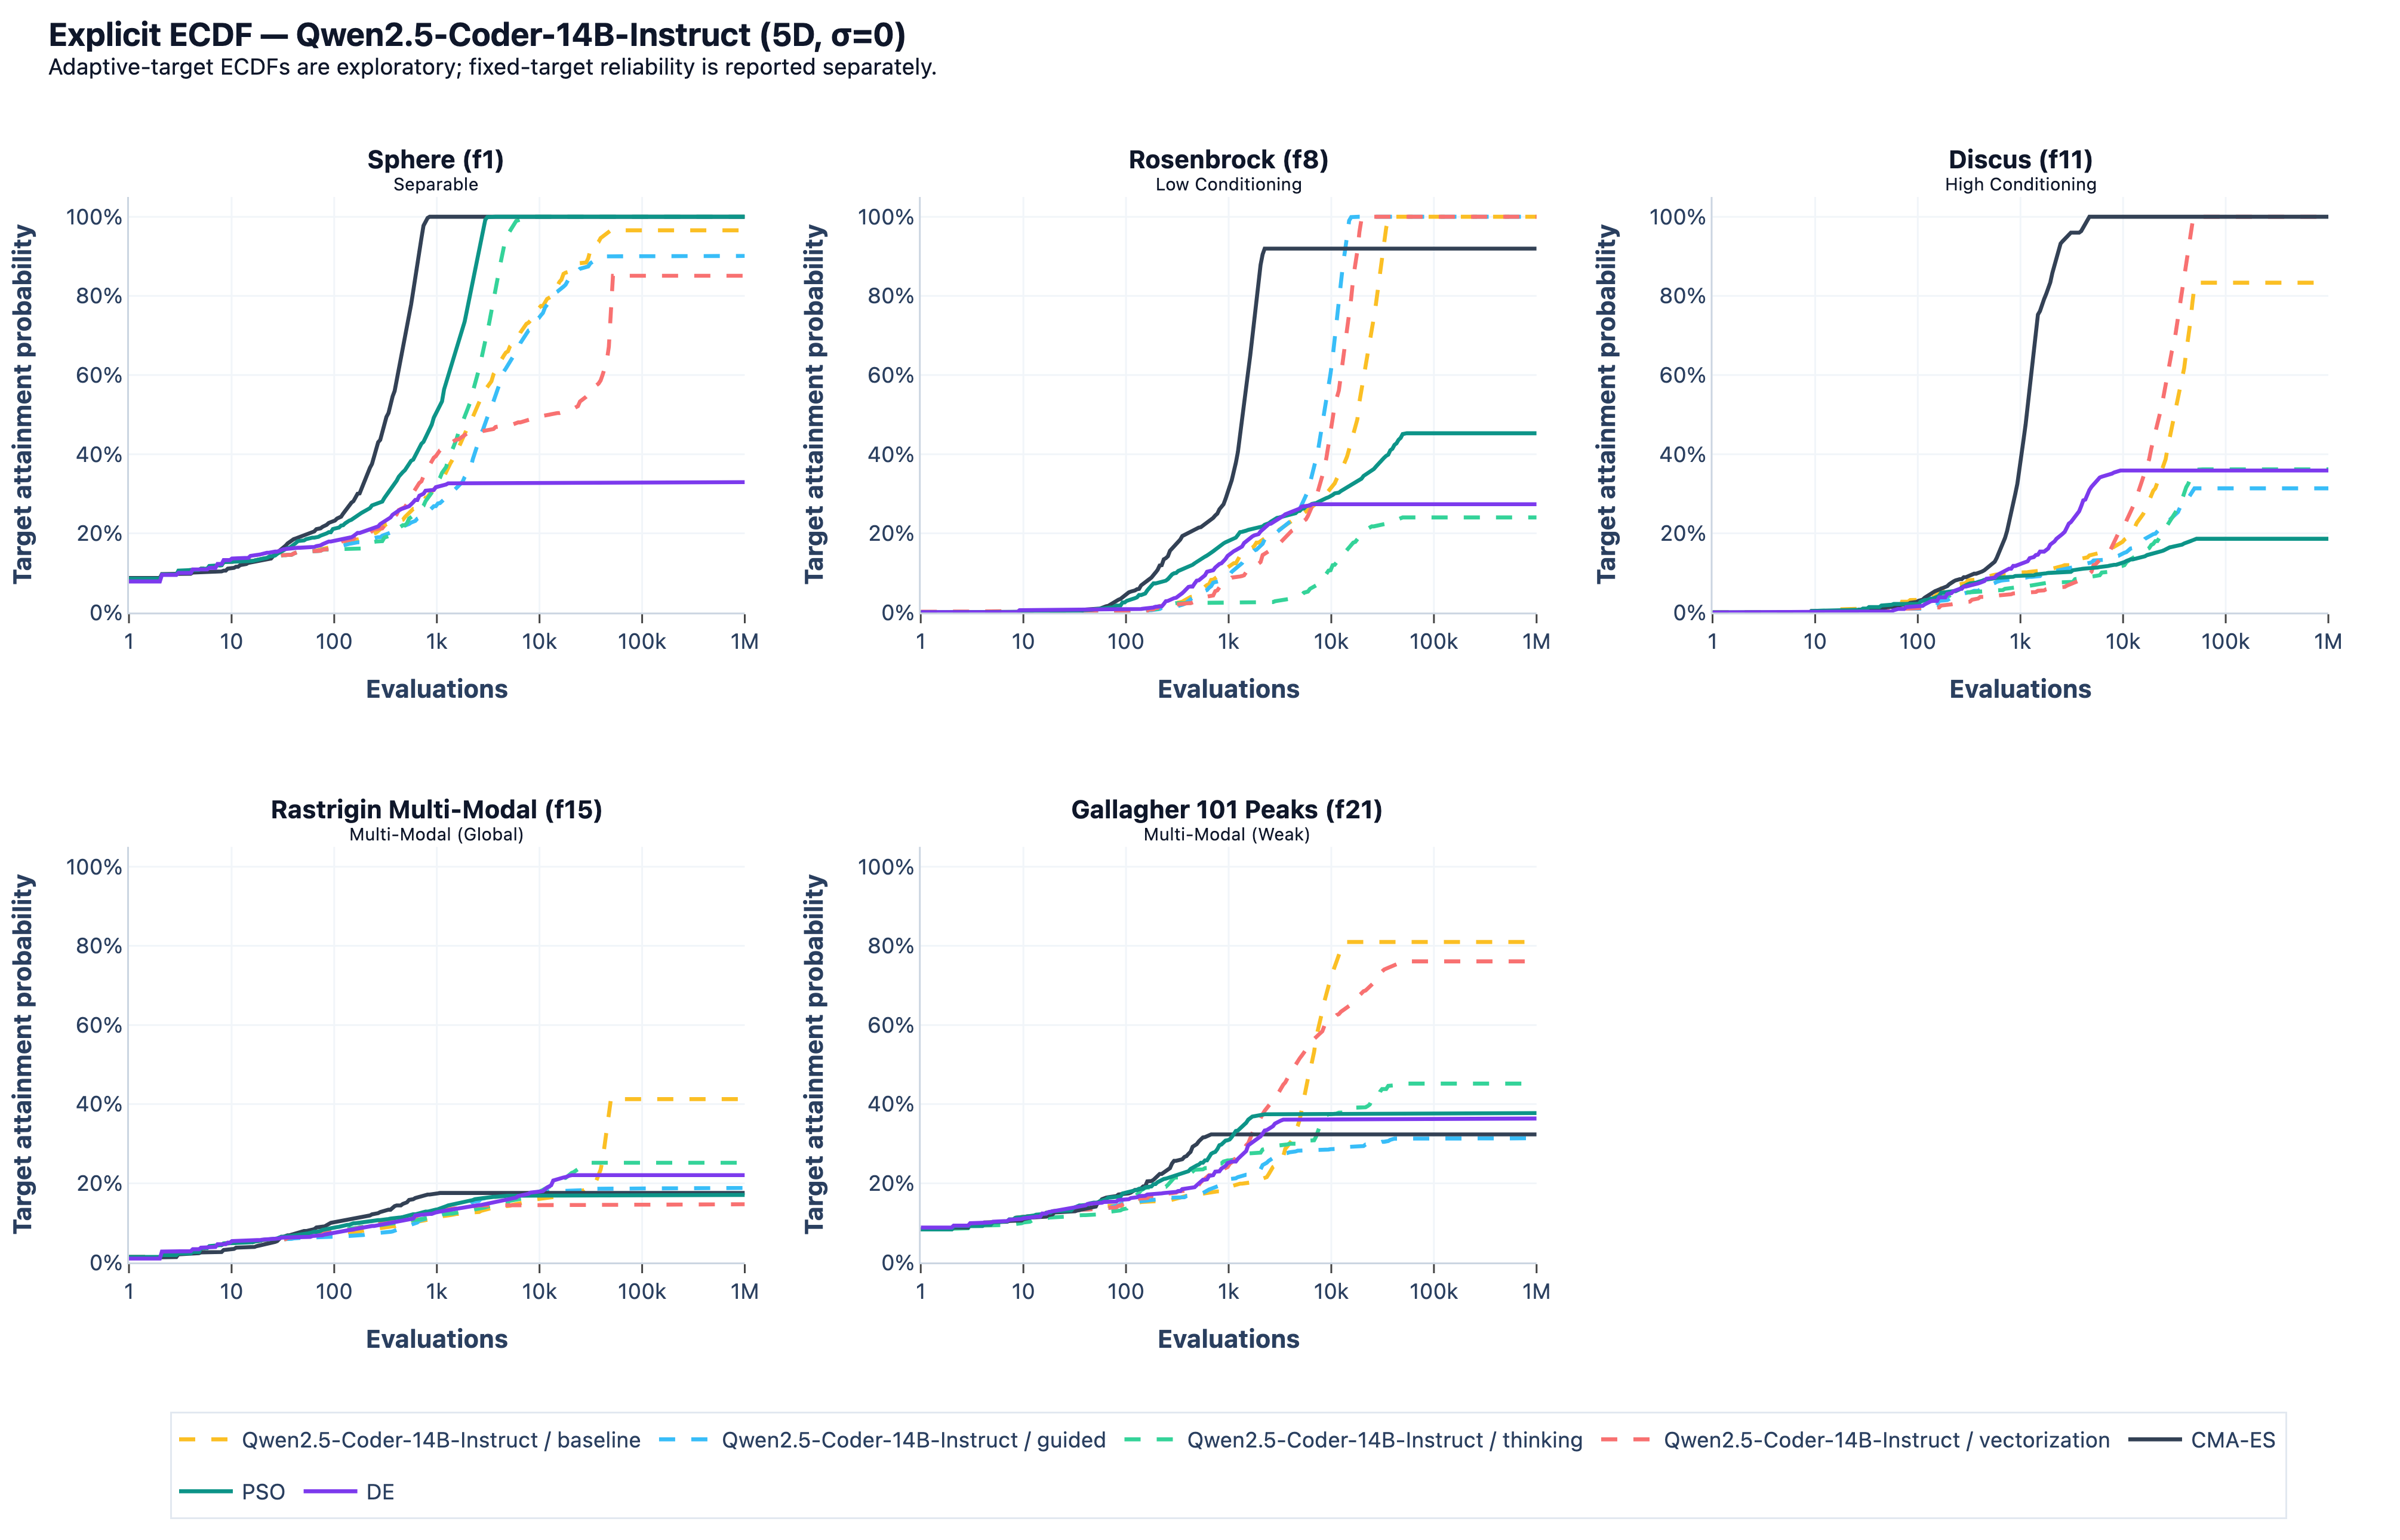
\includegraphics[width=\textwidth,height=0.32\textheight,keepaspectratio]{images/experiments/02_explicit/qwen_14b/5D/std_0.0/target_precision_ecdf.png}
    \caption{Qwen2.5-Coder-14B-Instruct: Explicit, $D=5$,
    $\sigma=0.0$. Convergence (median and IQR) above;
    adaptive target-precision ECDF below. The objective-query allowance
    is 50,000.}
    \label{fig:appendix_02_explicit_qwen_14b_5_std_00}
\end{minipage}
\par\medskip

\par\smallskip\noindent
\begin{minipage}{\linewidth}
    \captionsetup{type=figure,aboveskip=4pt,belowskip=0pt}
    \centering
    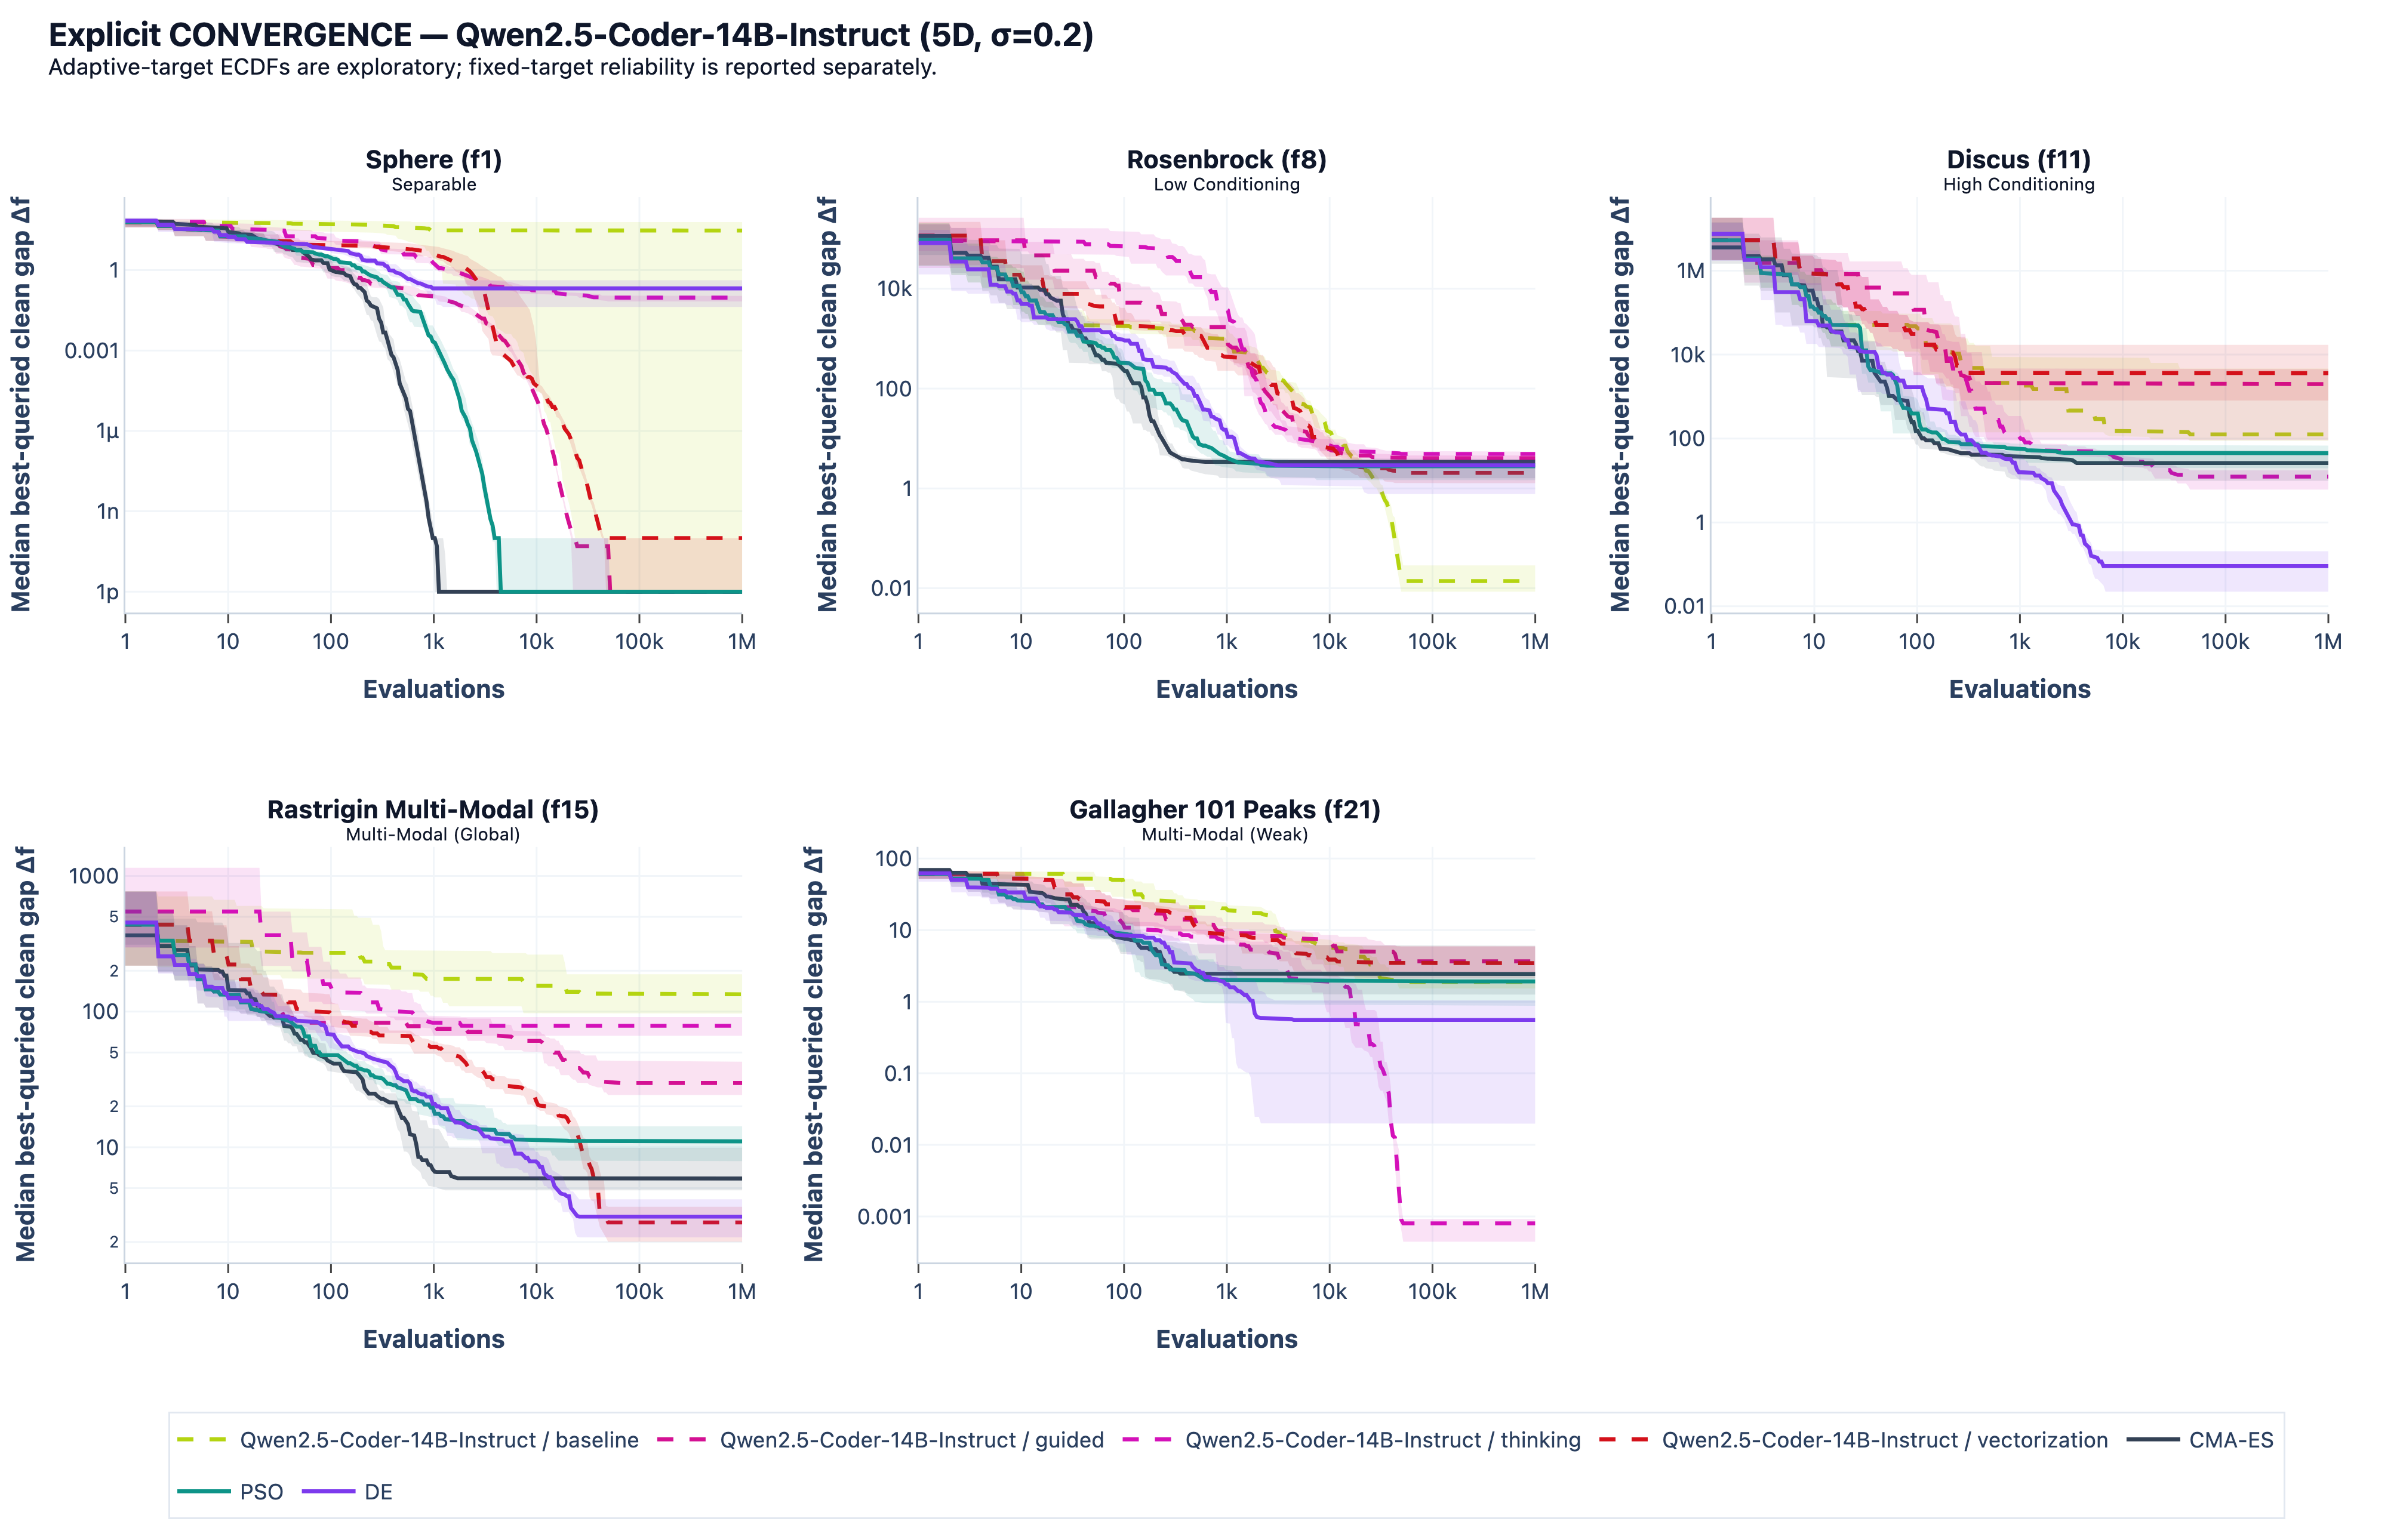
\includegraphics[width=\textwidth,height=0.32\textheight,keepaspectratio]{images/experiments/02_explicit/qwen_14b/5D/std_0.2/convergence_trajectories.png}
    \par\medskip
    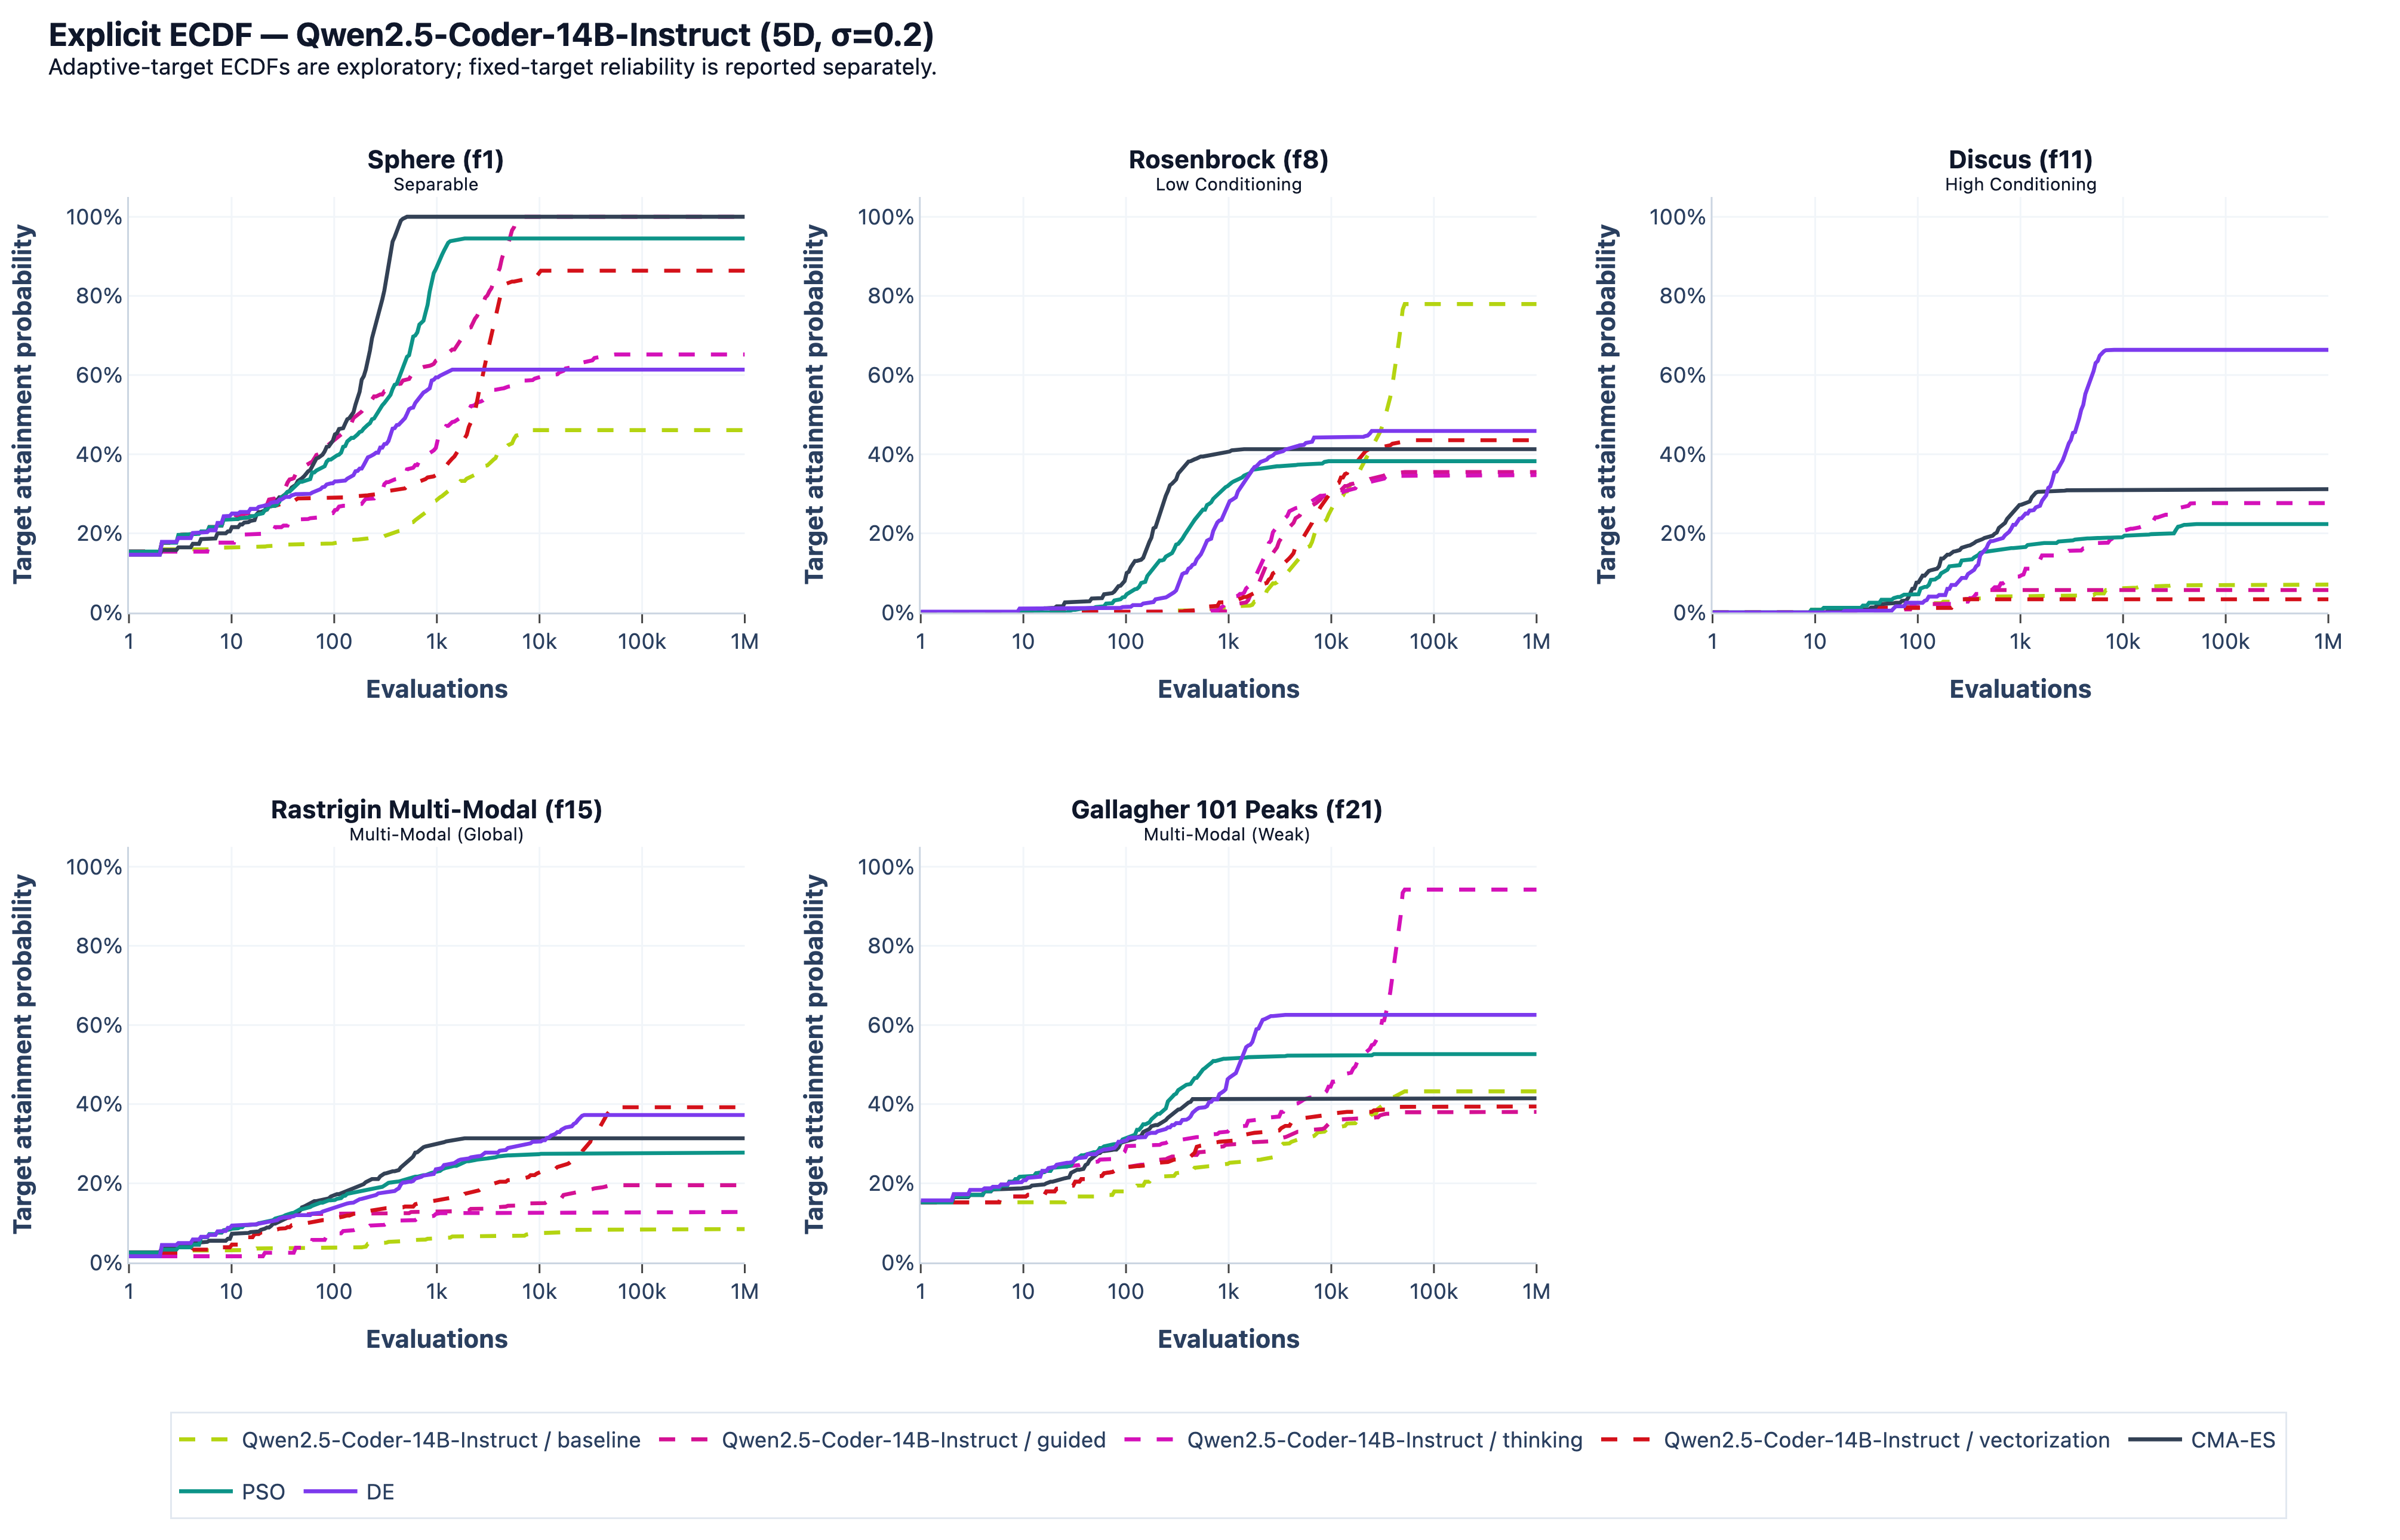
\includegraphics[width=\textwidth,height=0.32\textheight,keepaspectratio]{images/experiments/02_explicit/qwen_14b/5D/std_0.2/target_precision_ecdf.png}
    \caption{Qwen2.5-Coder-14B-Instruct: Explicit, $D=5$,
    $\sigma=0.2$. Convergence (median and IQR) above;
    adaptive target-precision ECDF below. The objective-query allowance
    is 50,000.}
    \label{fig:appendix_02_explicit_qwen_14b_5_std_02}
\end{minipage}
\par\medskip

\subsection{Qwen2.5-Coder-32B-Instruct}
\nopagebreak[4]

\par\smallskip\noindent
\begin{minipage}{\linewidth}
    \captionsetup{type=figure,aboveskip=4pt,belowskip=0pt}
    \centering
    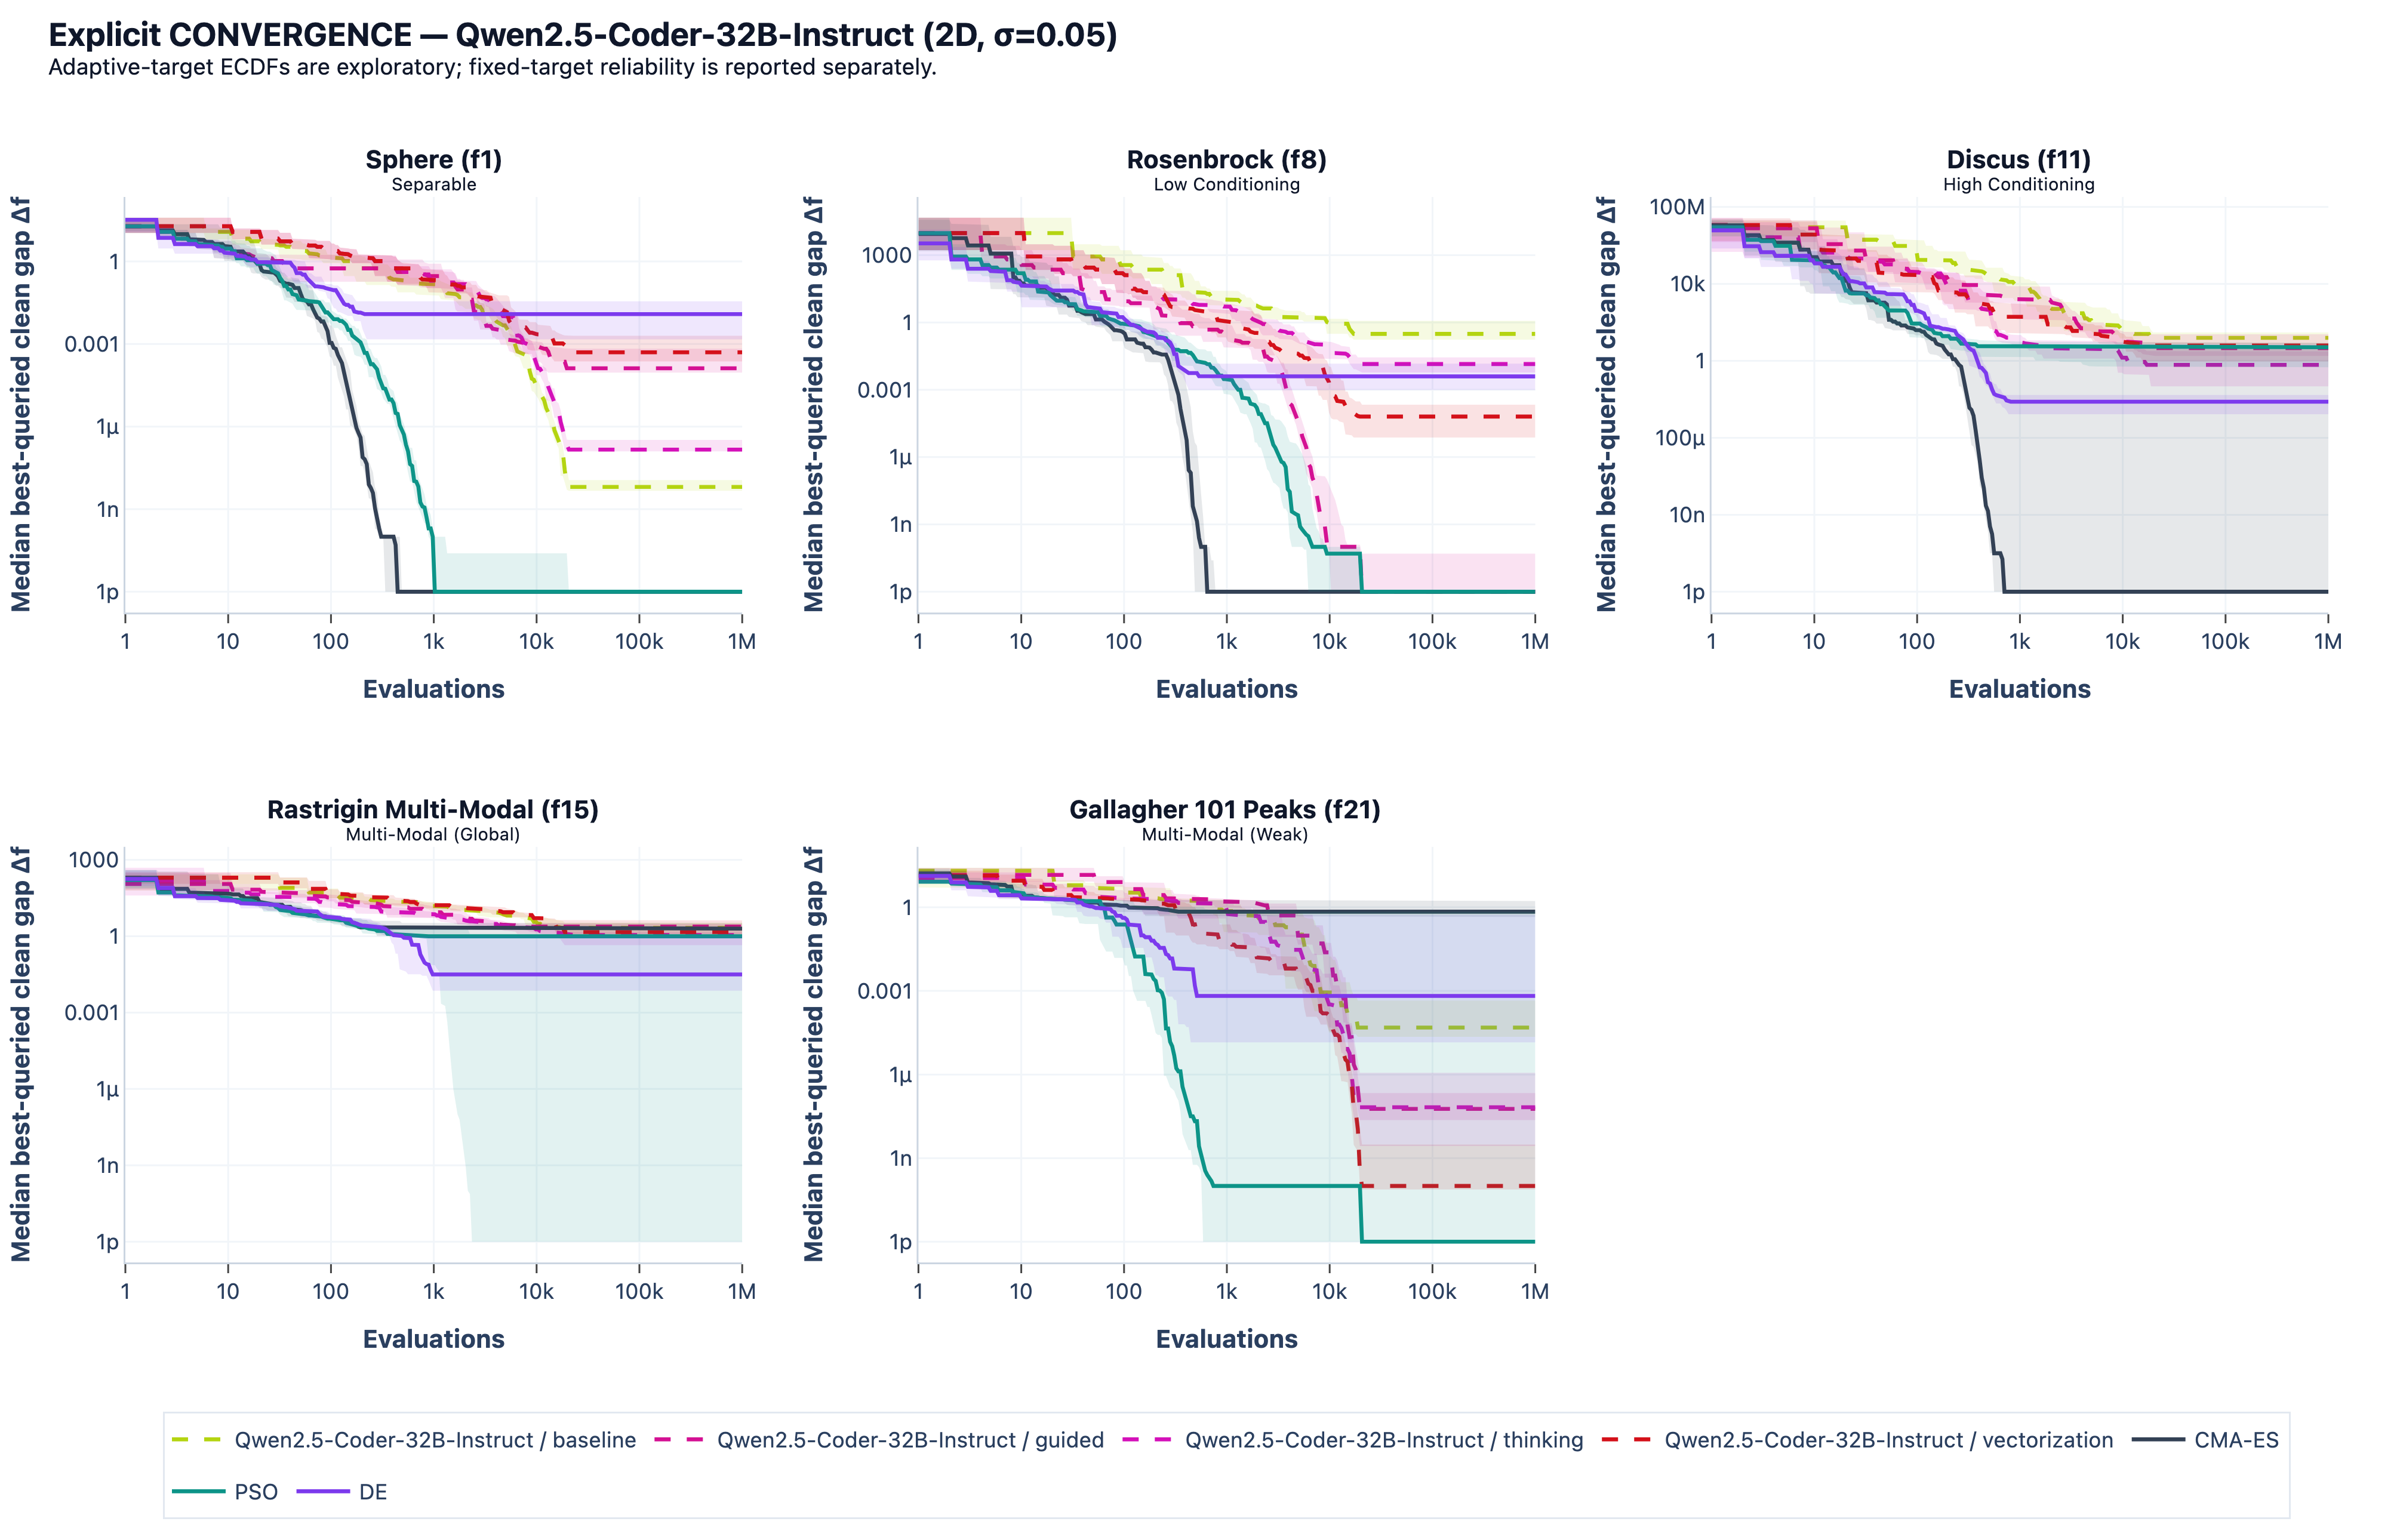
\includegraphics[width=\textwidth,height=0.32\textheight,keepaspectratio]{images/experiments/02_explicit/qwen_32b/2D/std_0.05/convergence_trajectories.png}
    \par\medskip
    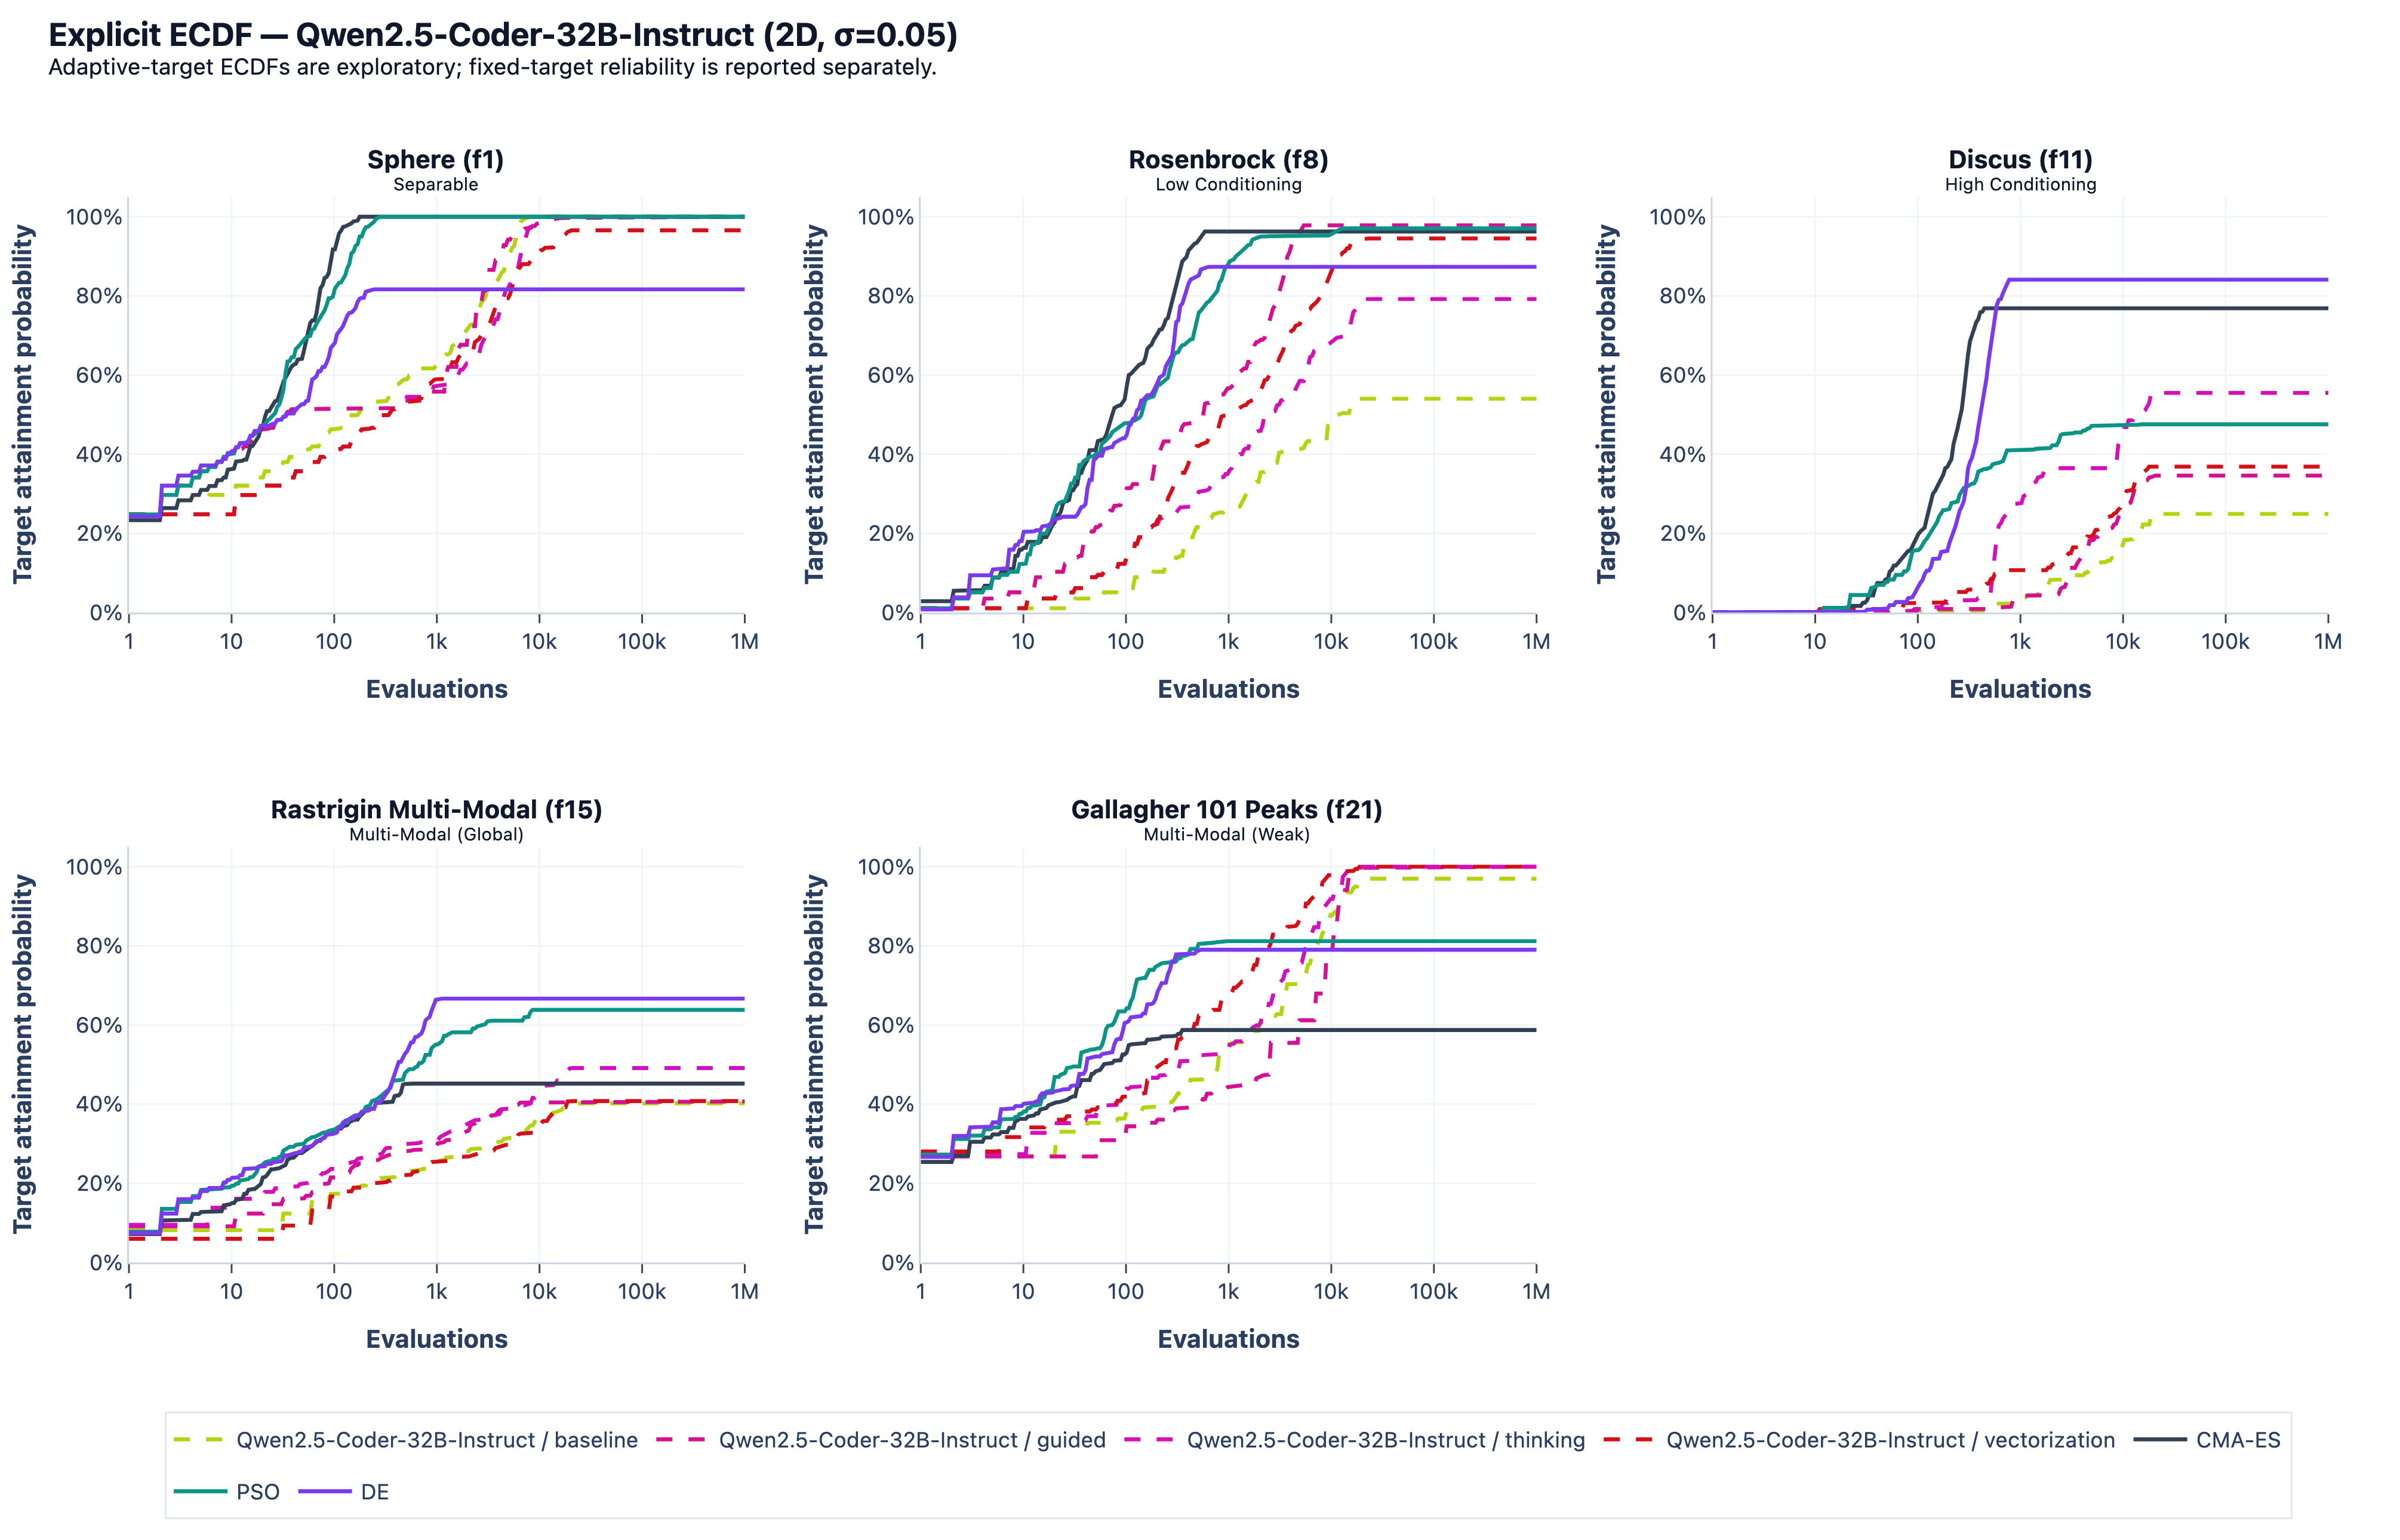
\includegraphics[width=\textwidth,height=0.32\textheight,keepaspectratio]{images/experiments/02_explicit/qwen_32b/2D/std_0.05/target_precision_ecdf.png}
    \caption{Qwen2.5-Coder-32B-Instruct: Explicit, $D=2$,
    $\sigma=0.05$. Convergence (median and IQR) above;
    adaptive target-precision ECDF below. The objective-query allowance
    is 20,000.}
    \label{fig:appendix_02_explicit_qwen_32b_2_std_005}
\end{minipage}
\par\medskip

\par\smallskip\noindent
\begin{minipage}{\linewidth}
    \captionsetup{type=figure,aboveskip=4pt,belowskip=0pt}
    \centering
    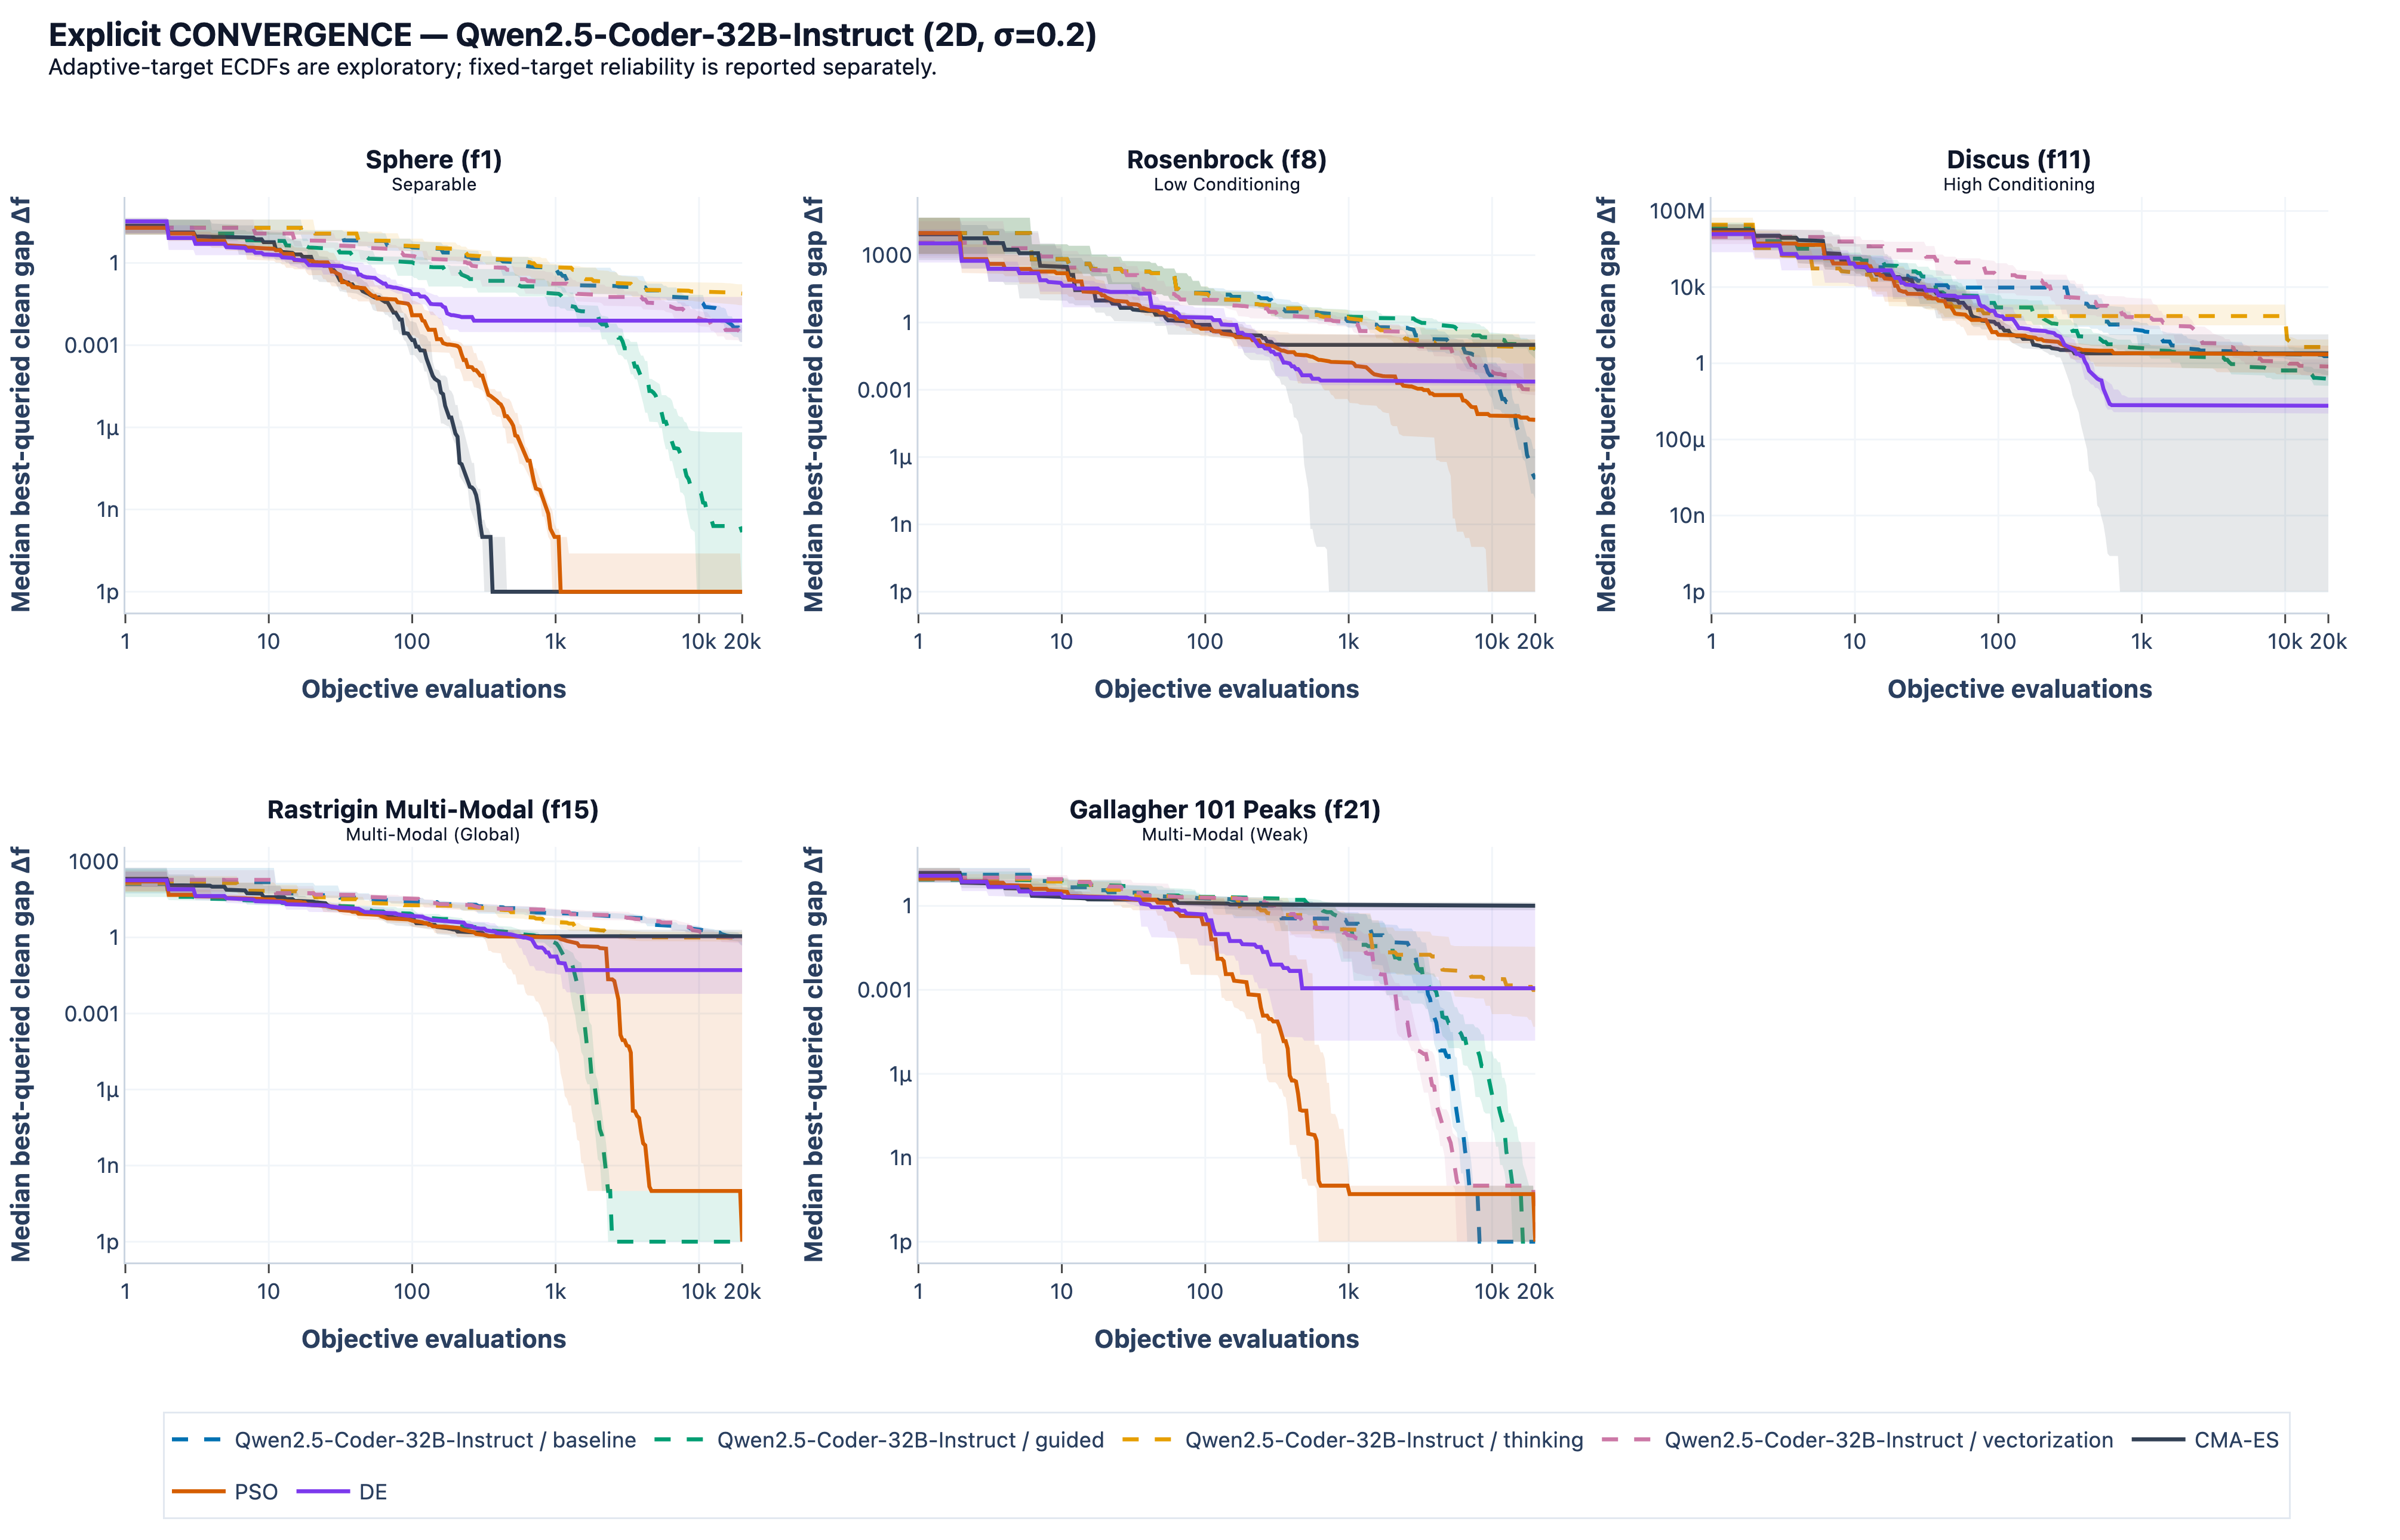
\includegraphics[width=\textwidth,height=0.32\textheight,keepaspectratio]{images/experiments/02_explicit/qwen_32b/2D/std_0.2/convergence_trajectories.png}
    \par\medskip
    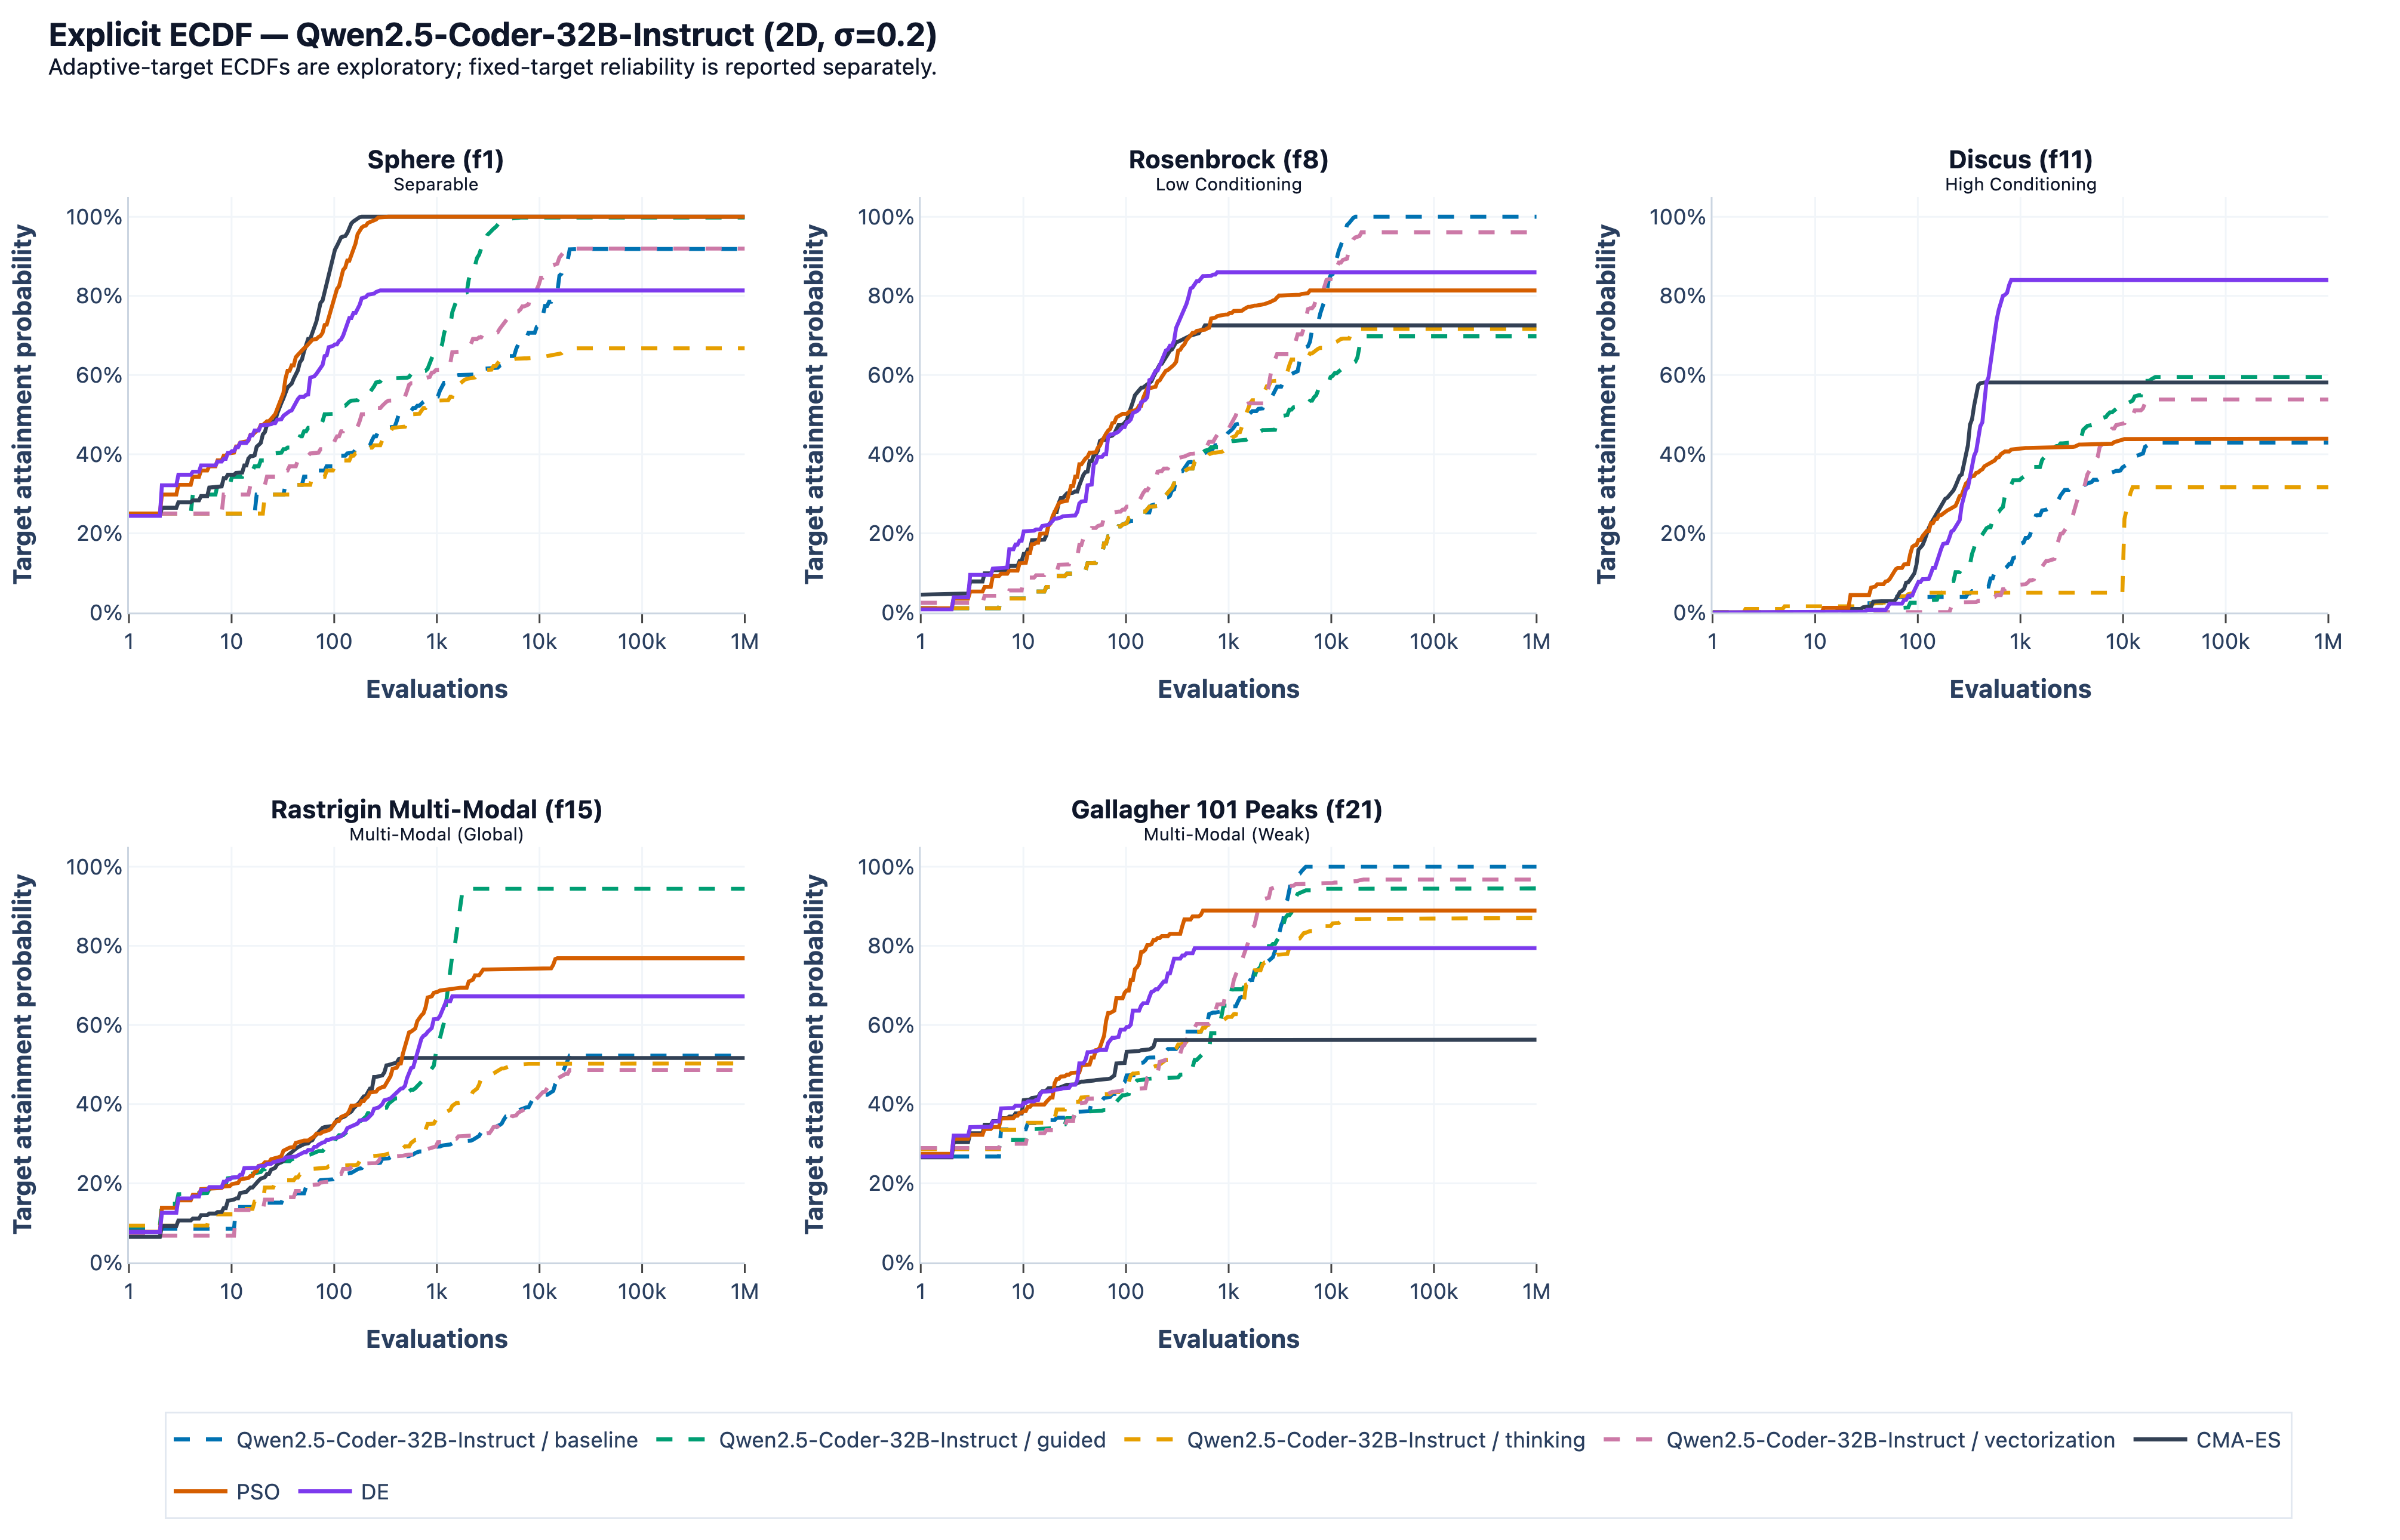
\includegraphics[width=\textwidth,height=0.32\textheight,keepaspectratio]{images/experiments/02_explicit/qwen_32b/2D/std_0.2/target_precision_ecdf.png}
    \caption{Qwen2.5-Coder-32B-Instruct: Explicit, $D=2$,
    $\sigma=0.2$. Convergence (median and IQR) above;
    adaptive target-precision ECDF below. The objective-query allowance
    is 20,000.}
    \label{fig:appendix_02_explicit_qwen_32b_2_std_02}
\end{minipage}
\par\medskip

\par\smallskip\noindent
\begin{minipage}{\linewidth}
    \captionsetup{type=figure,aboveskip=4pt,belowskip=0pt}
    \centering
    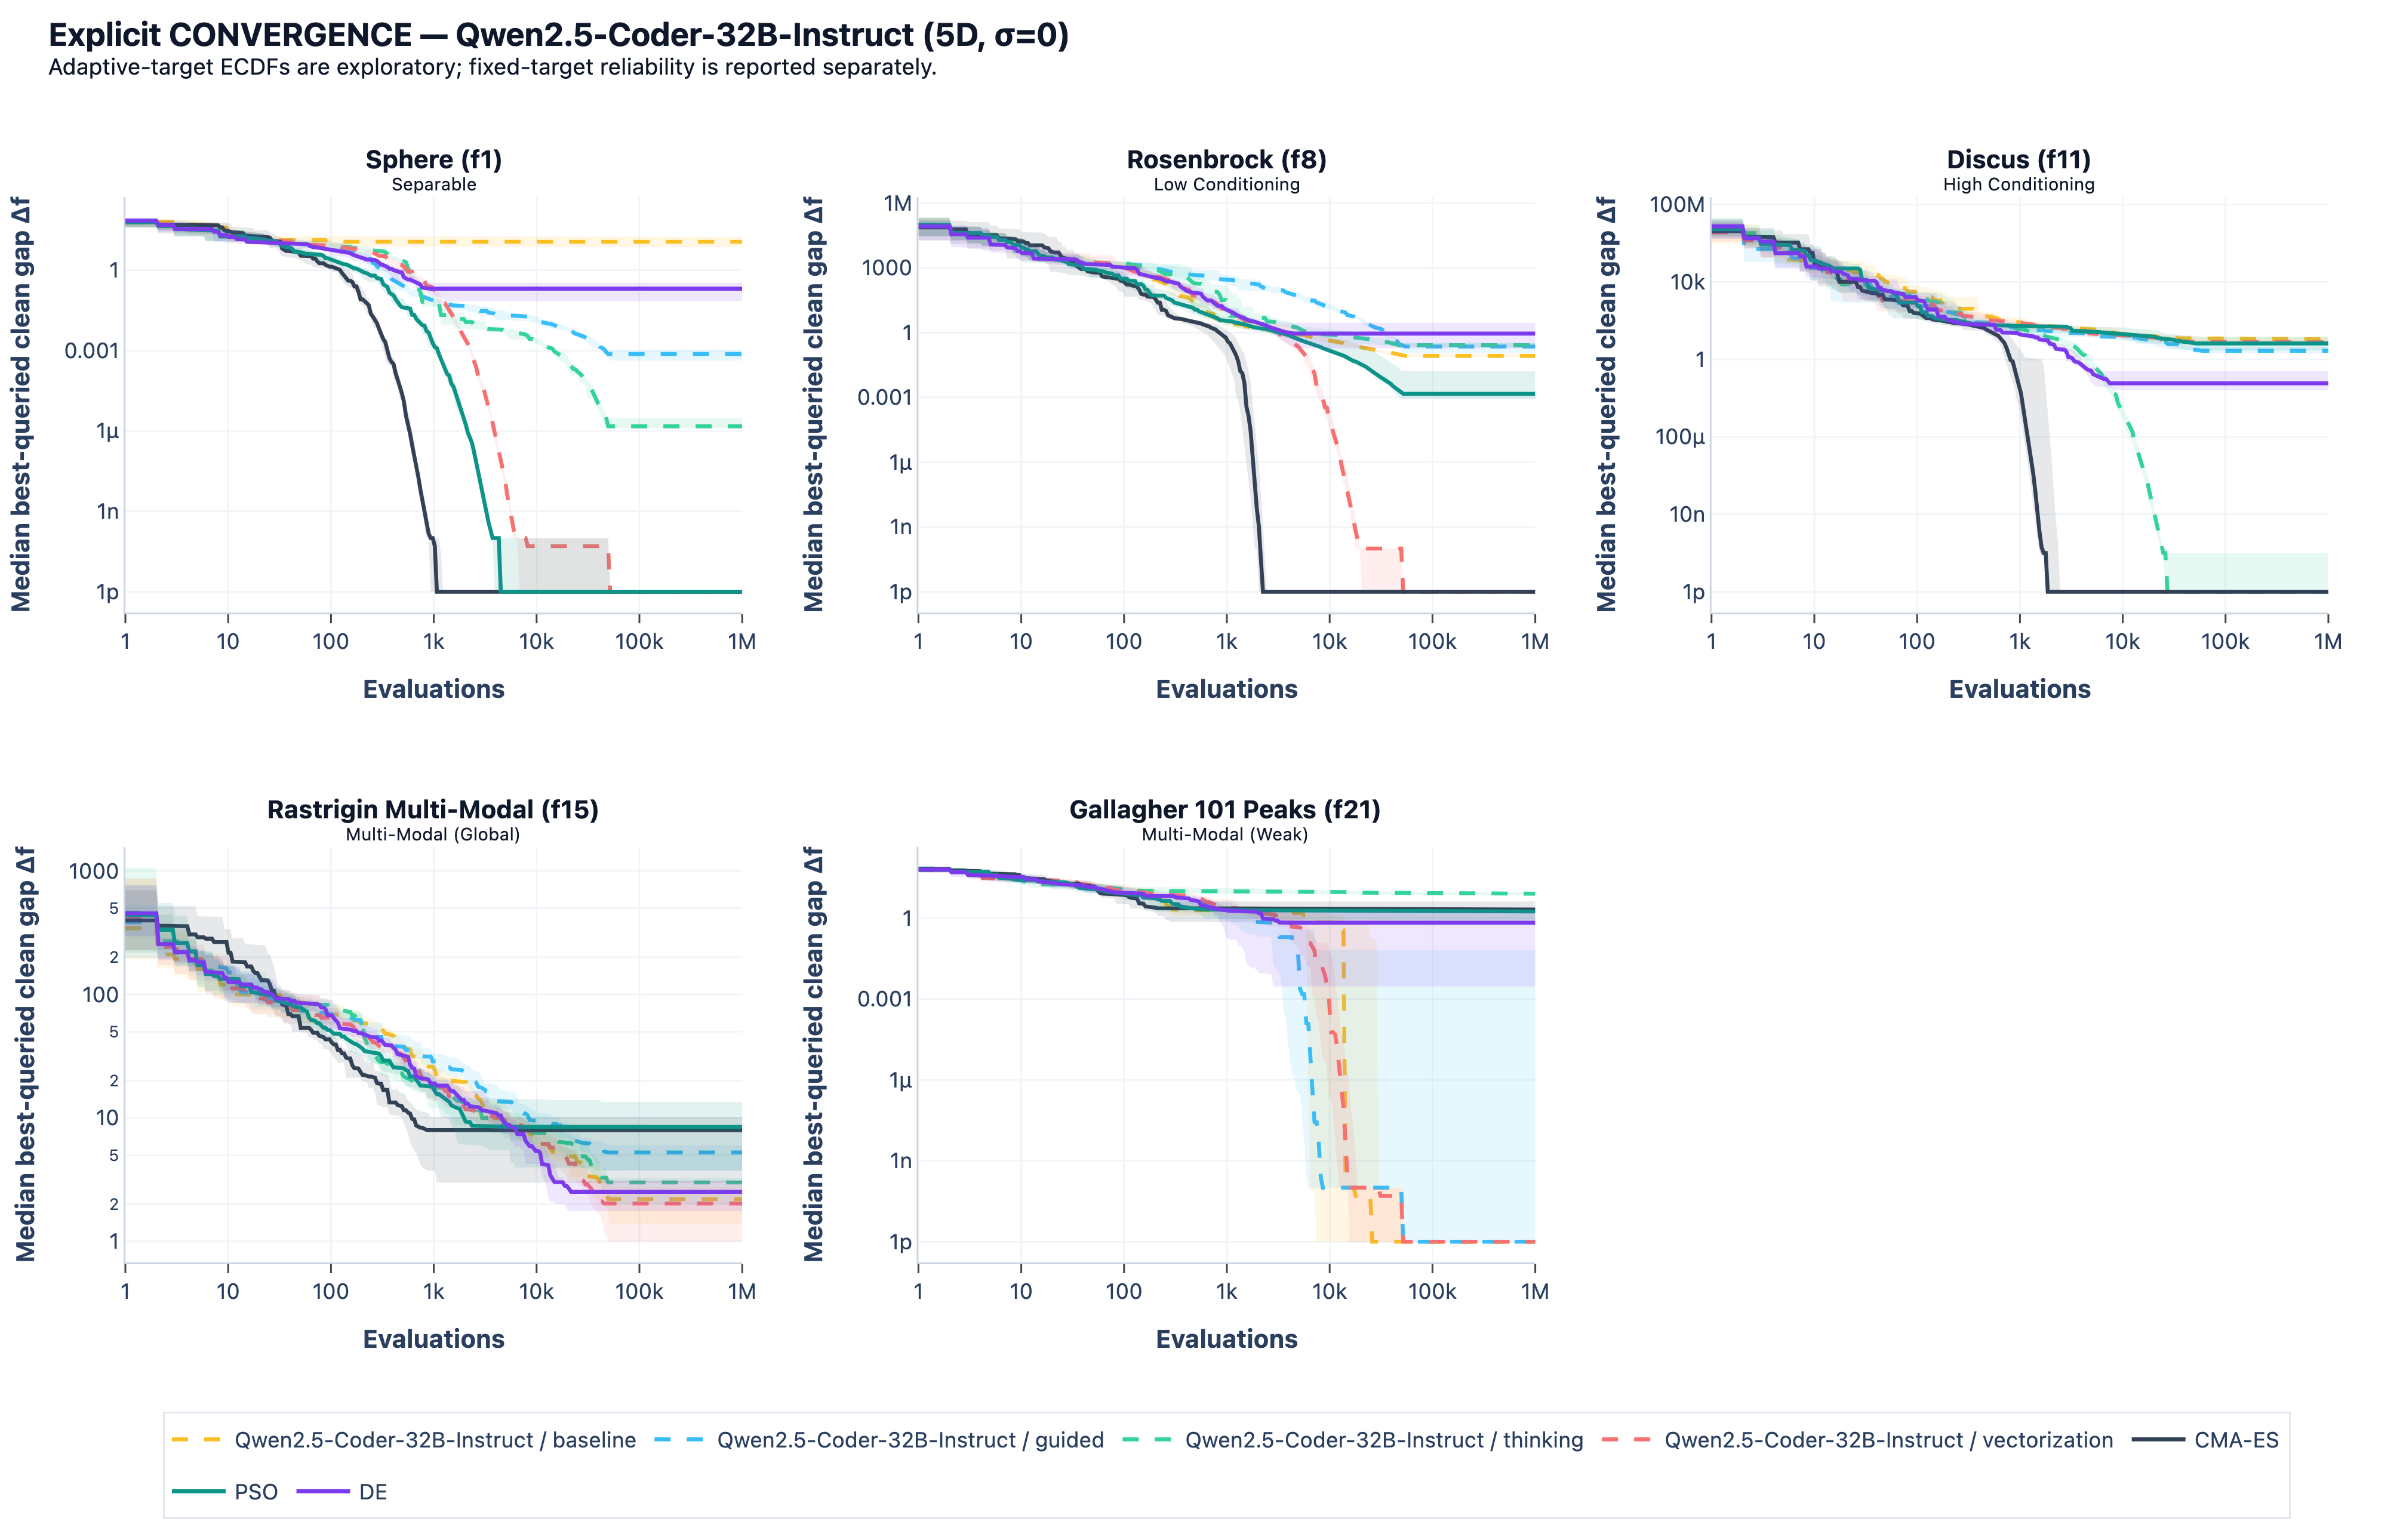
\includegraphics[width=\textwidth,height=0.32\textheight,keepaspectratio]{images/experiments/02_explicit/qwen_32b/5D/std_0.0/convergence_trajectories.png}
    \par\medskip
    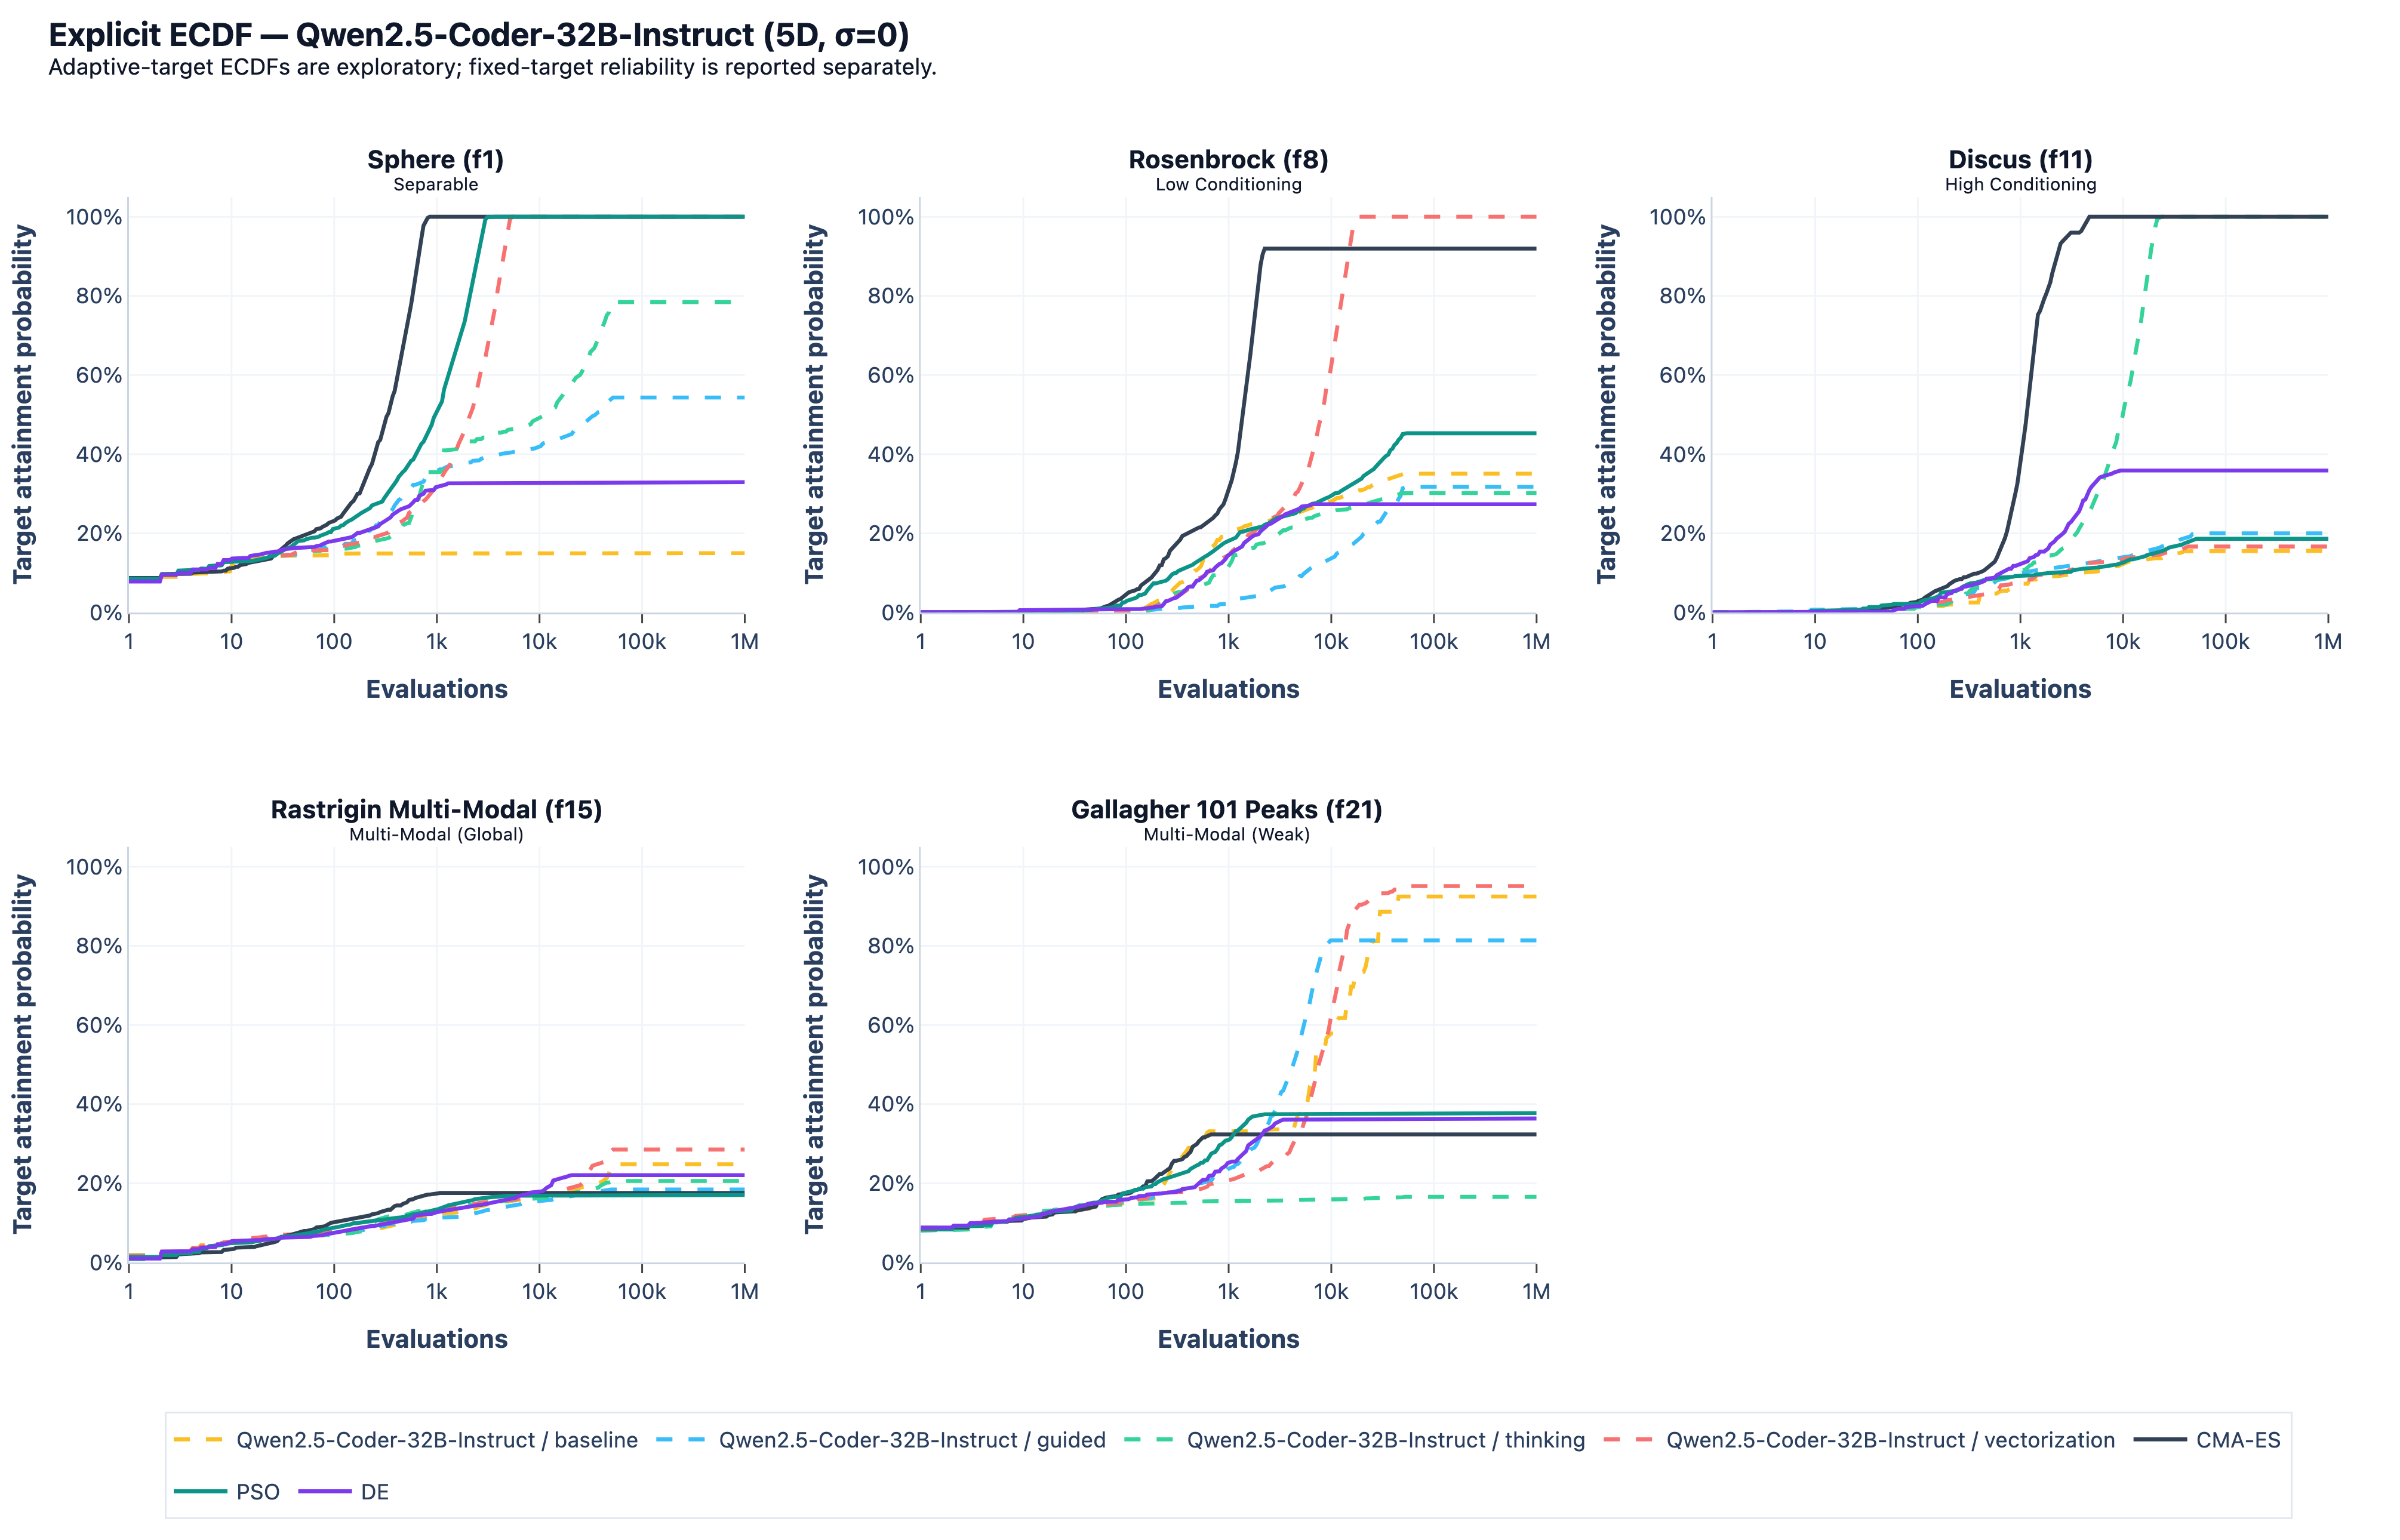
\includegraphics[width=\textwidth,height=0.32\textheight,keepaspectratio]{images/experiments/02_explicit/qwen_32b/5D/std_0.0/target_precision_ecdf.png}
    \caption{Qwen2.5-Coder-32B-Instruct: Explicit, $D=5$,
    $\sigma=0.0$. Convergence (median and IQR) above;
    adaptive target-precision ECDF below. The objective-query allowance
    is 50,000.}
    \label{fig:appendix_02_explicit_qwen_32b_5_std_00}
\end{minipage}
\par\medskip

\par\smallskip\noindent
\begin{minipage}{\linewidth}
    \captionsetup{type=figure,aboveskip=4pt,belowskip=0pt}
    \centering
    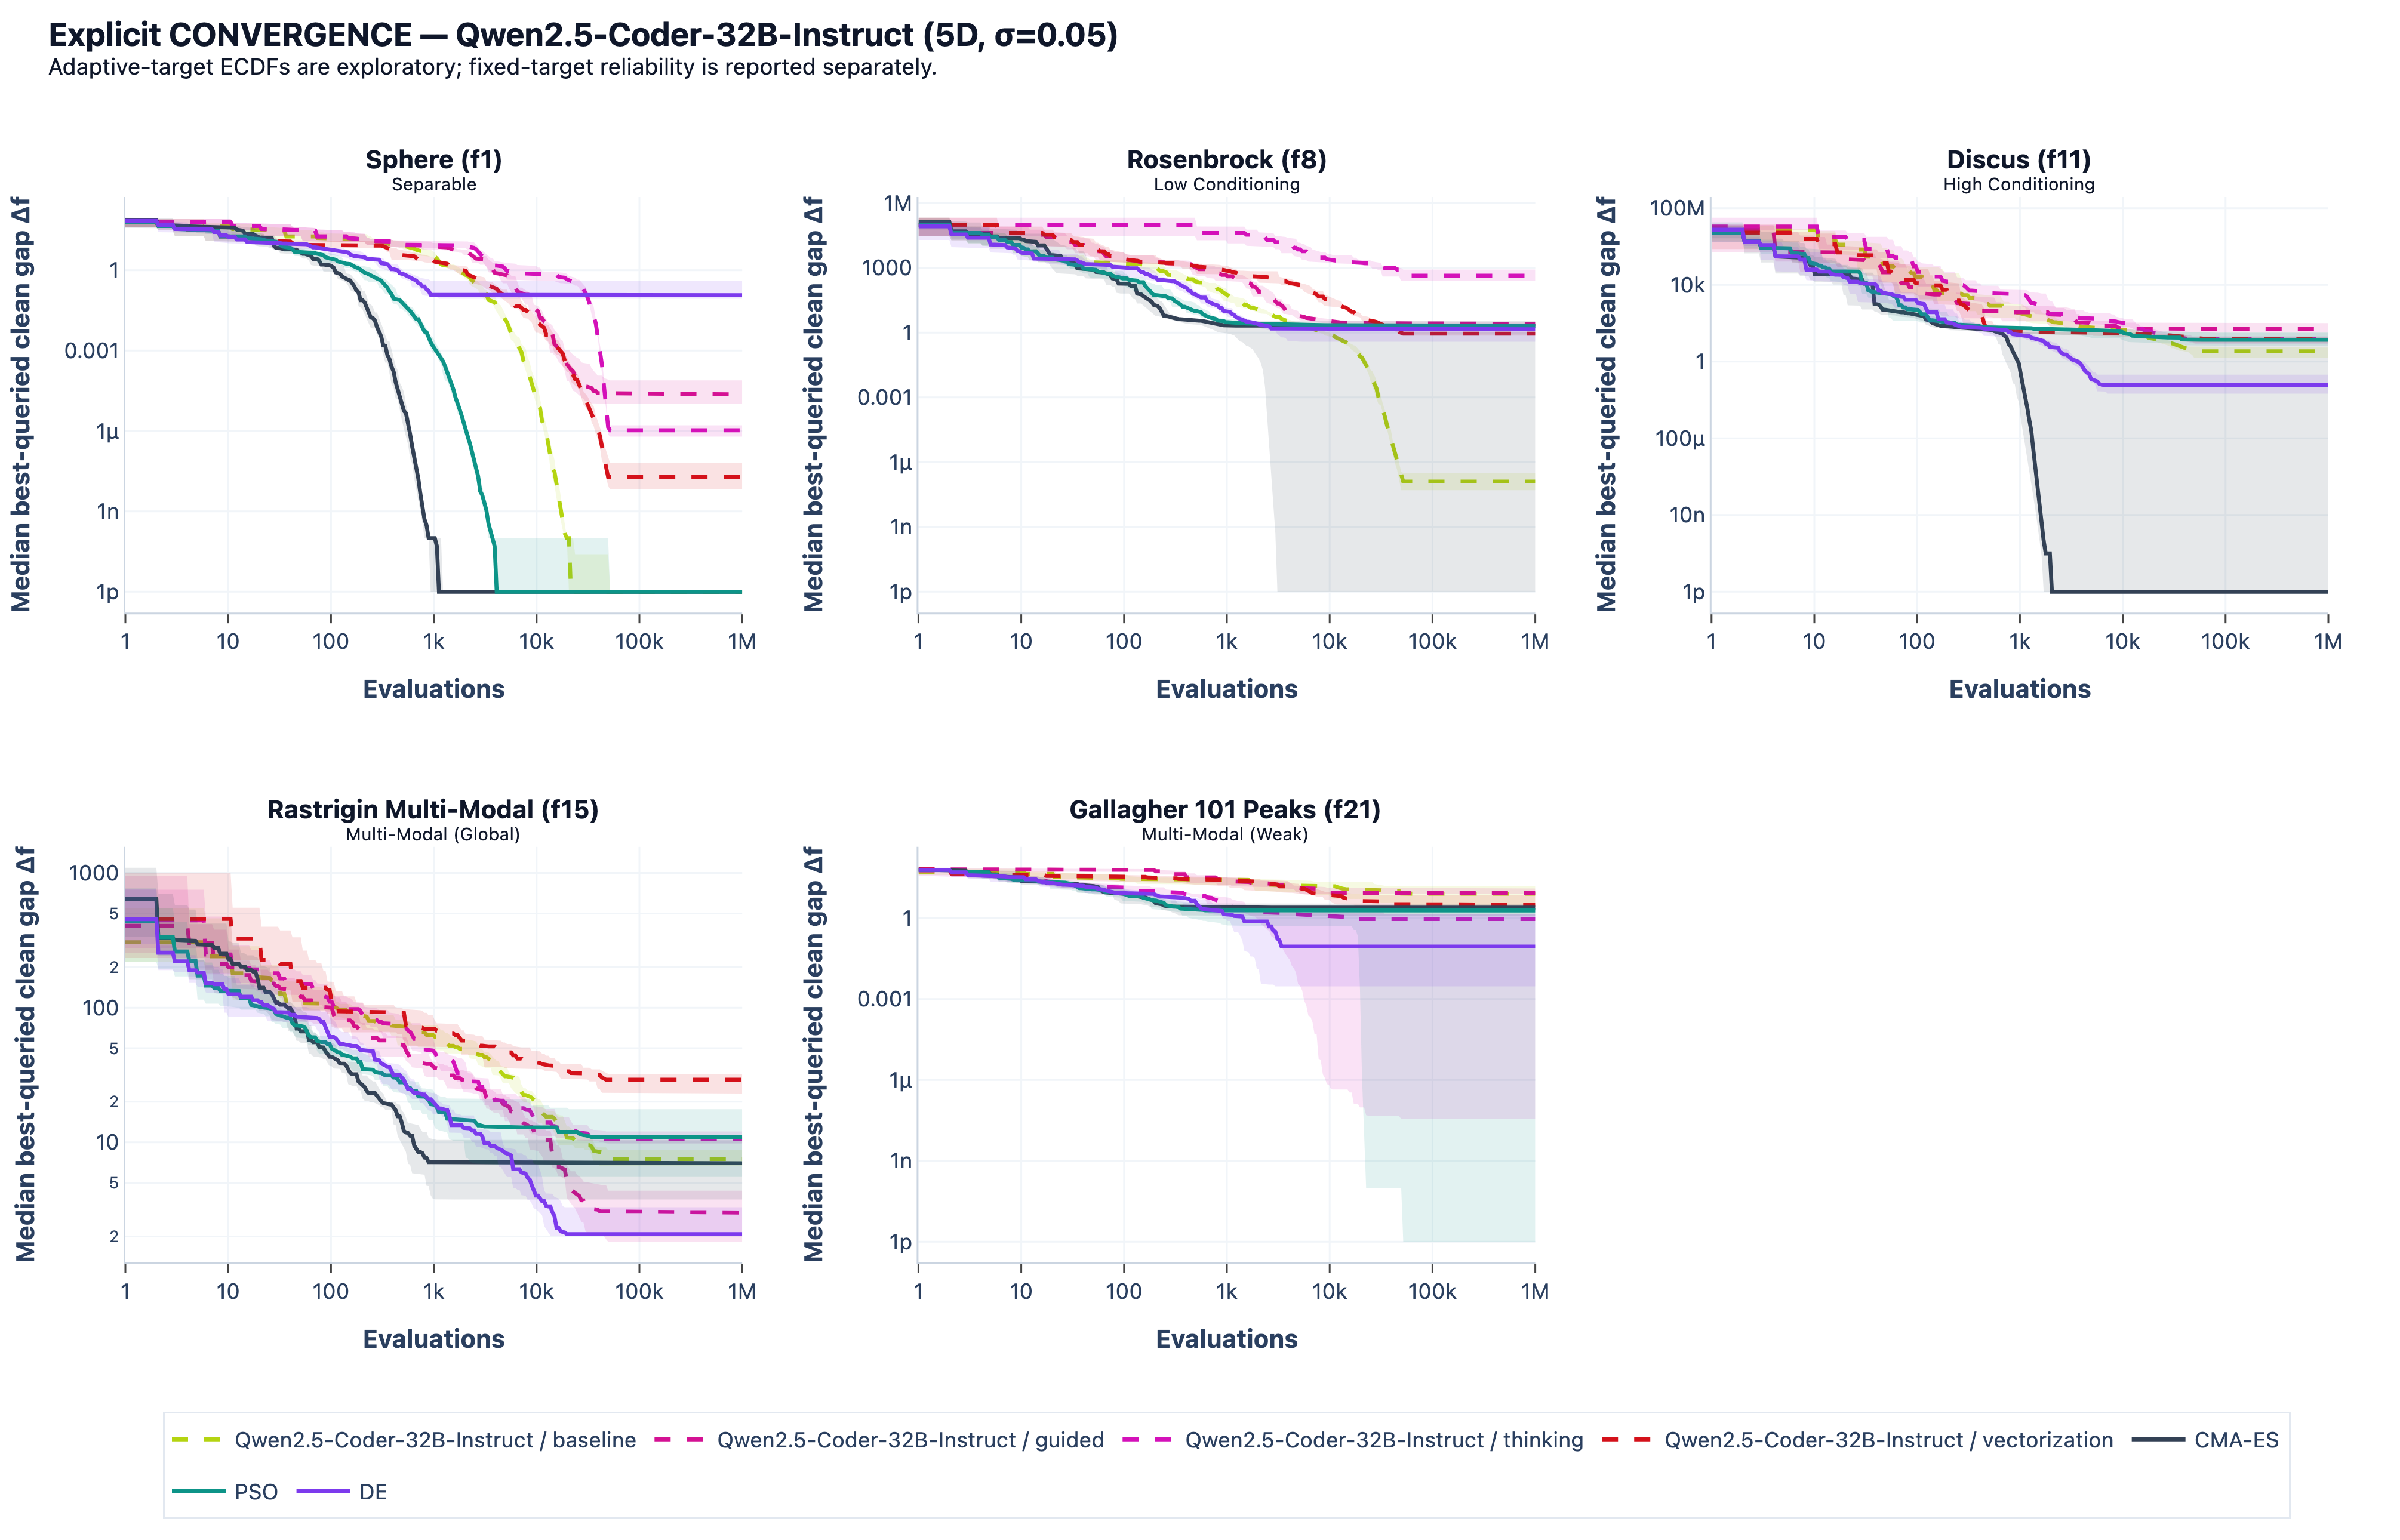
\includegraphics[width=\textwidth,height=0.32\textheight,keepaspectratio]{images/experiments/02_explicit/qwen_32b/5D/std_0.05/convergence_trajectories.png}
    \par\medskip
    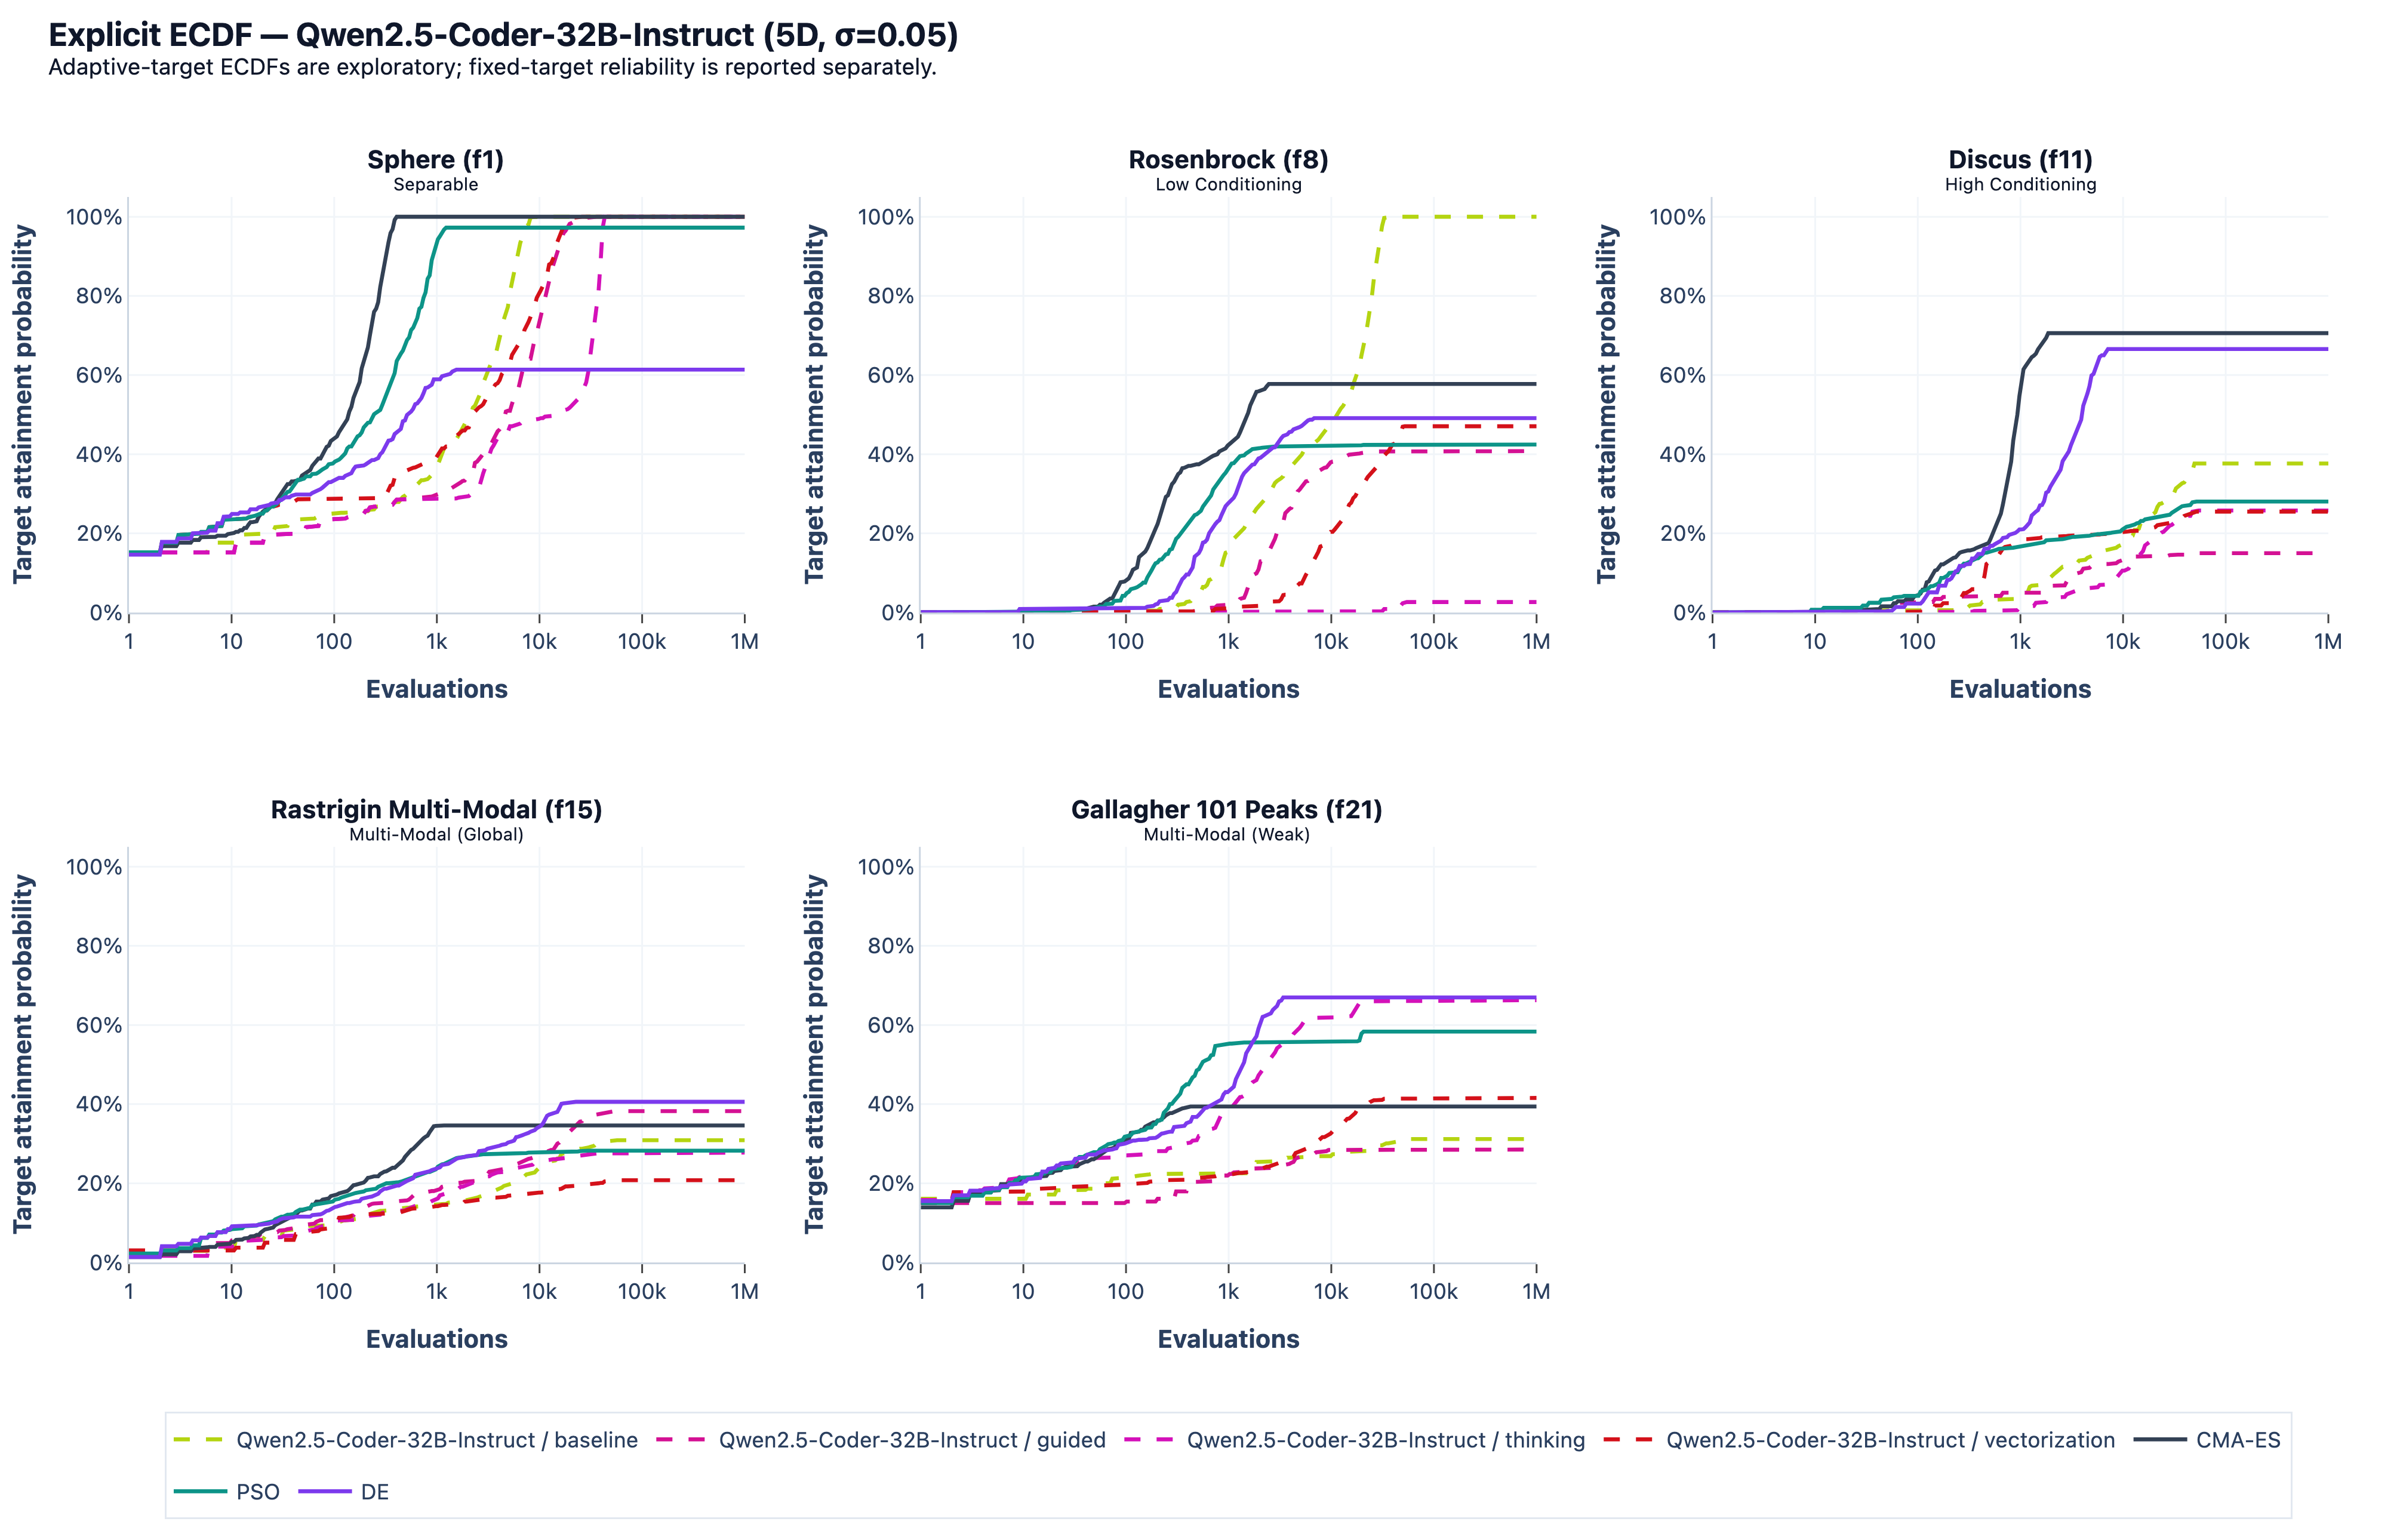
\includegraphics[width=\textwidth,height=0.32\textheight,keepaspectratio]{images/experiments/02_explicit/qwen_32b/5D/std_0.05/target_precision_ecdf.png}
    \caption{Qwen2.5-Coder-32B-Instruct: Explicit, $D=5$,
    $\sigma=0.05$. Convergence (median and IQR) above;
    adaptive target-precision ECDF below. The objective-query allowance
    is 50,000.}
    \label{fig:appendix_02_explicit_qwen_32b_5_std_005}
\end{minipage}
\par\medskip

\par\smallskip\noindent
\begin{minipage}{\linewidth}
    \captionsetup{type=figure,aboveskip=4pt,belowskip=0pt}
    \centering
    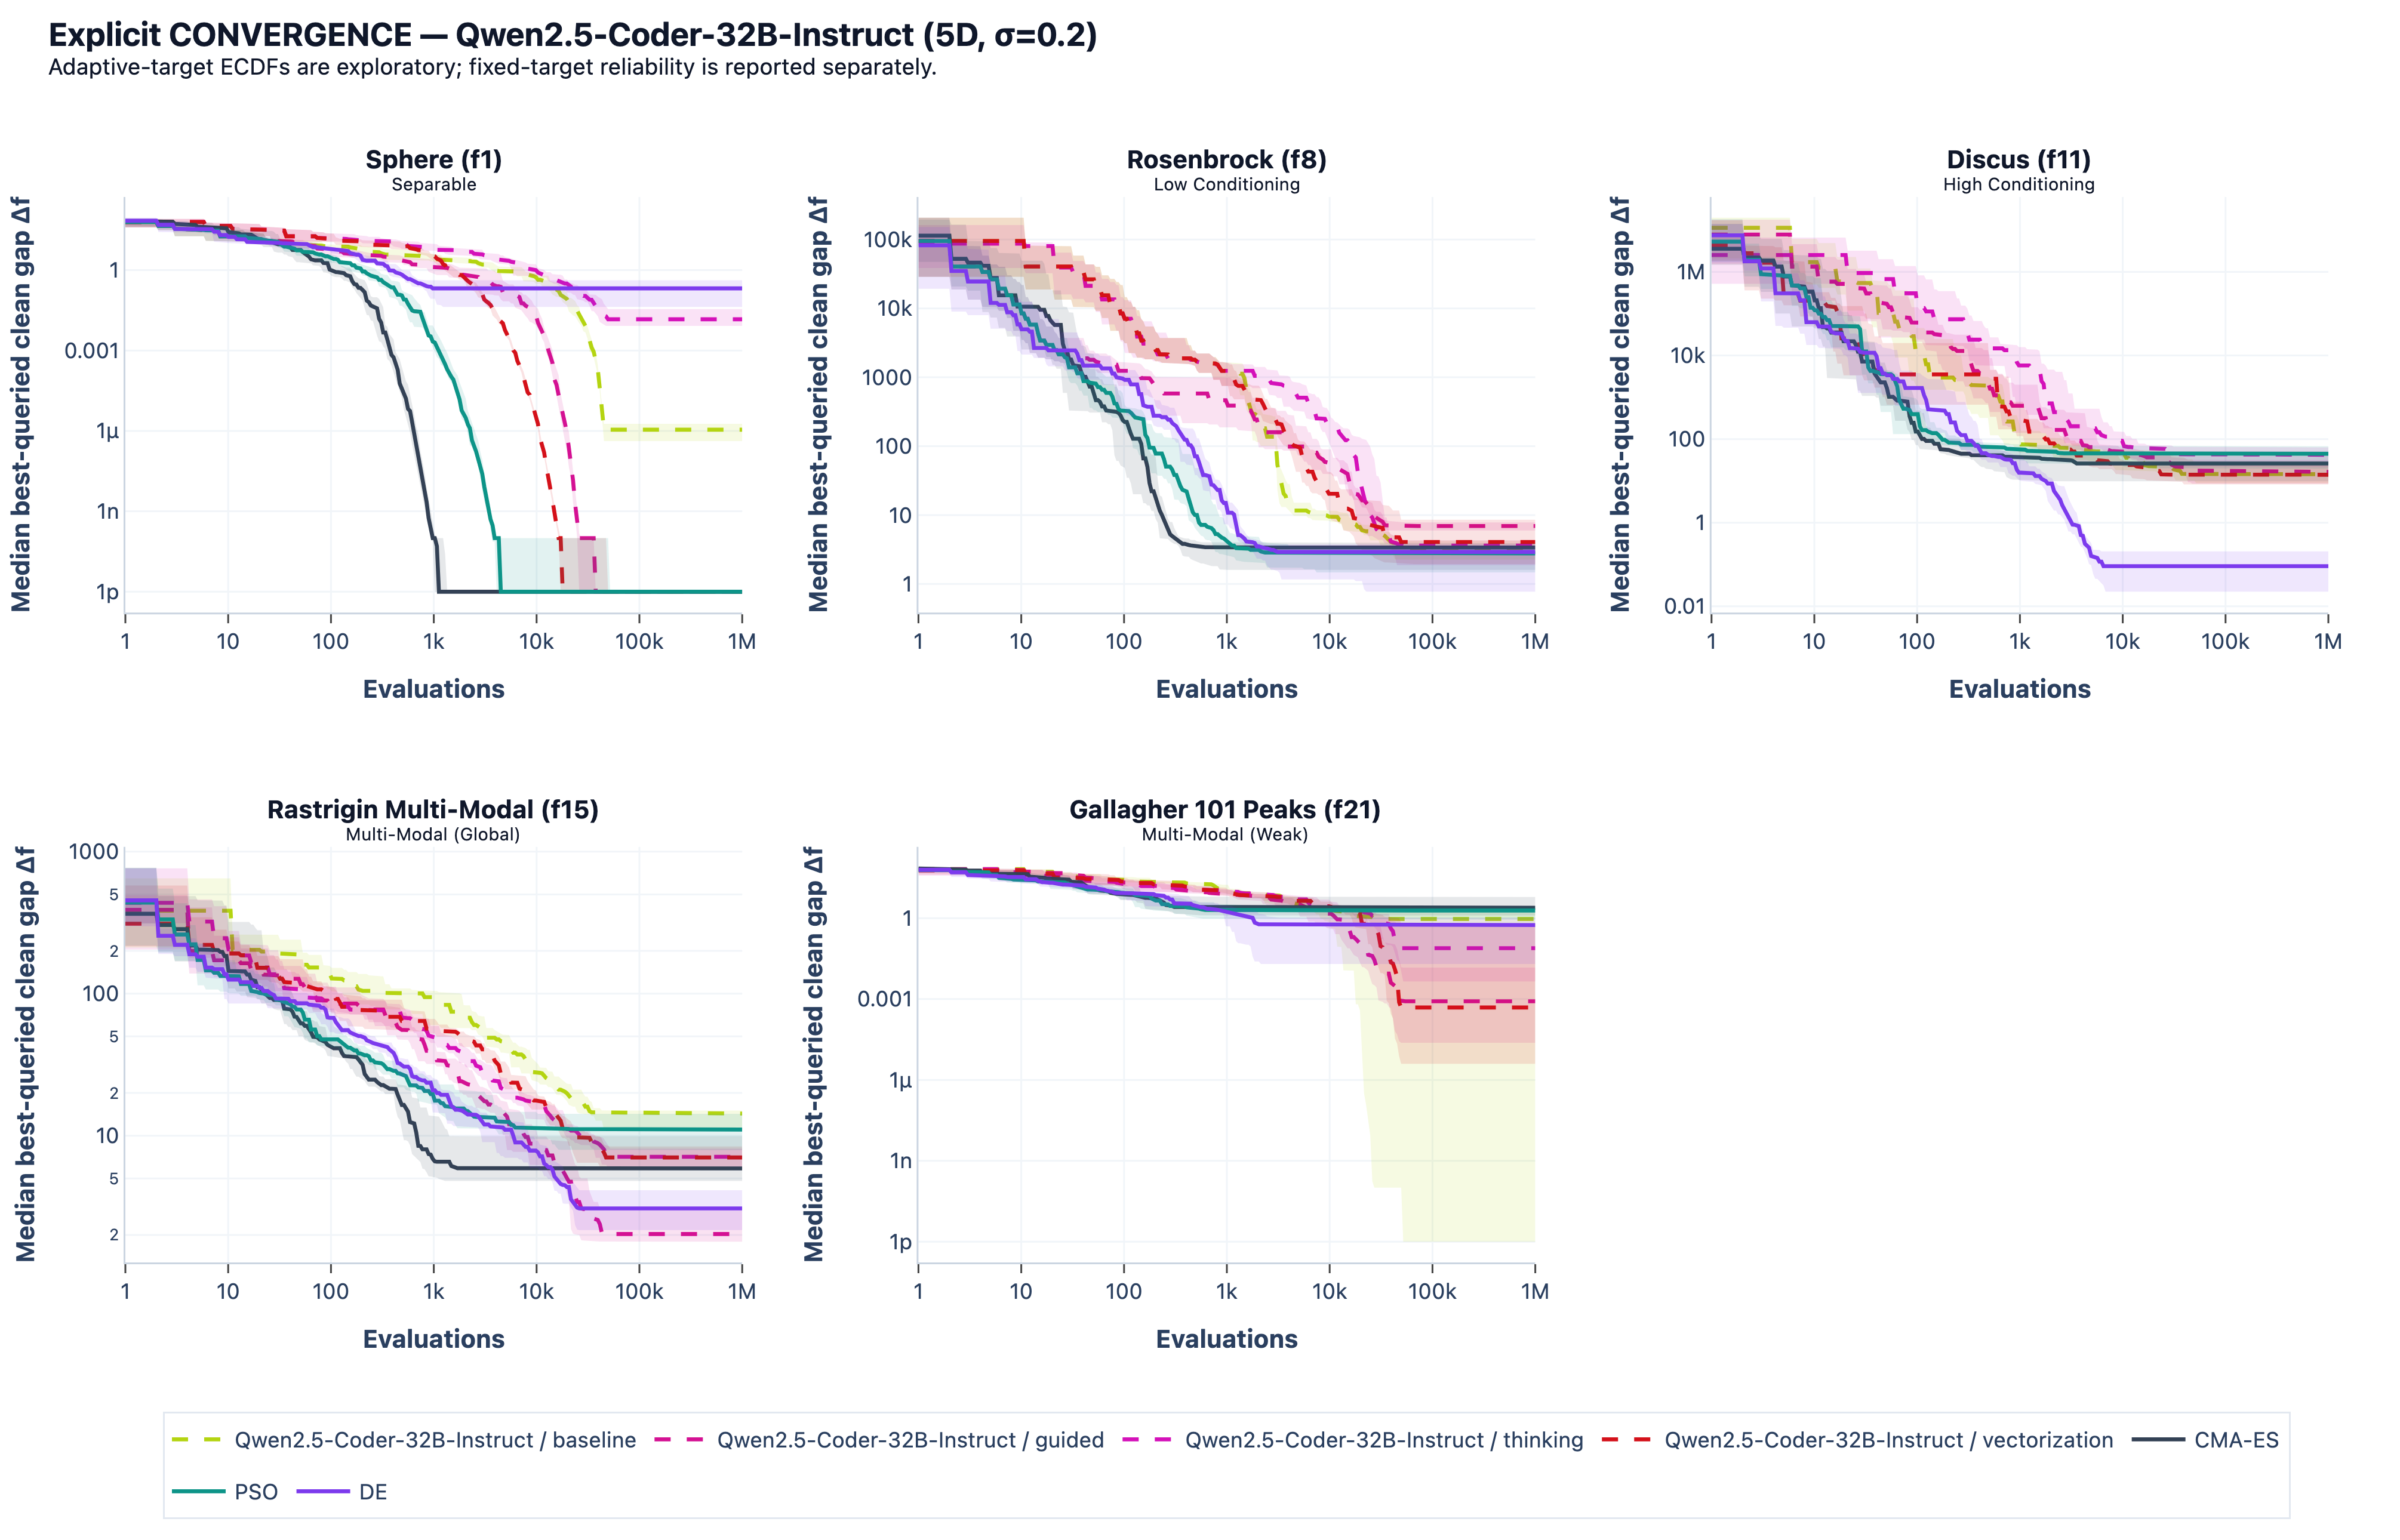
\includegraphics[width=\textwidth,height=0.32\textheight,keepaspectratio]{images/experiments/02_explicit/qwen_32b/5D/std_0.2/convergence_trajectories.png}
    \par\medskip
    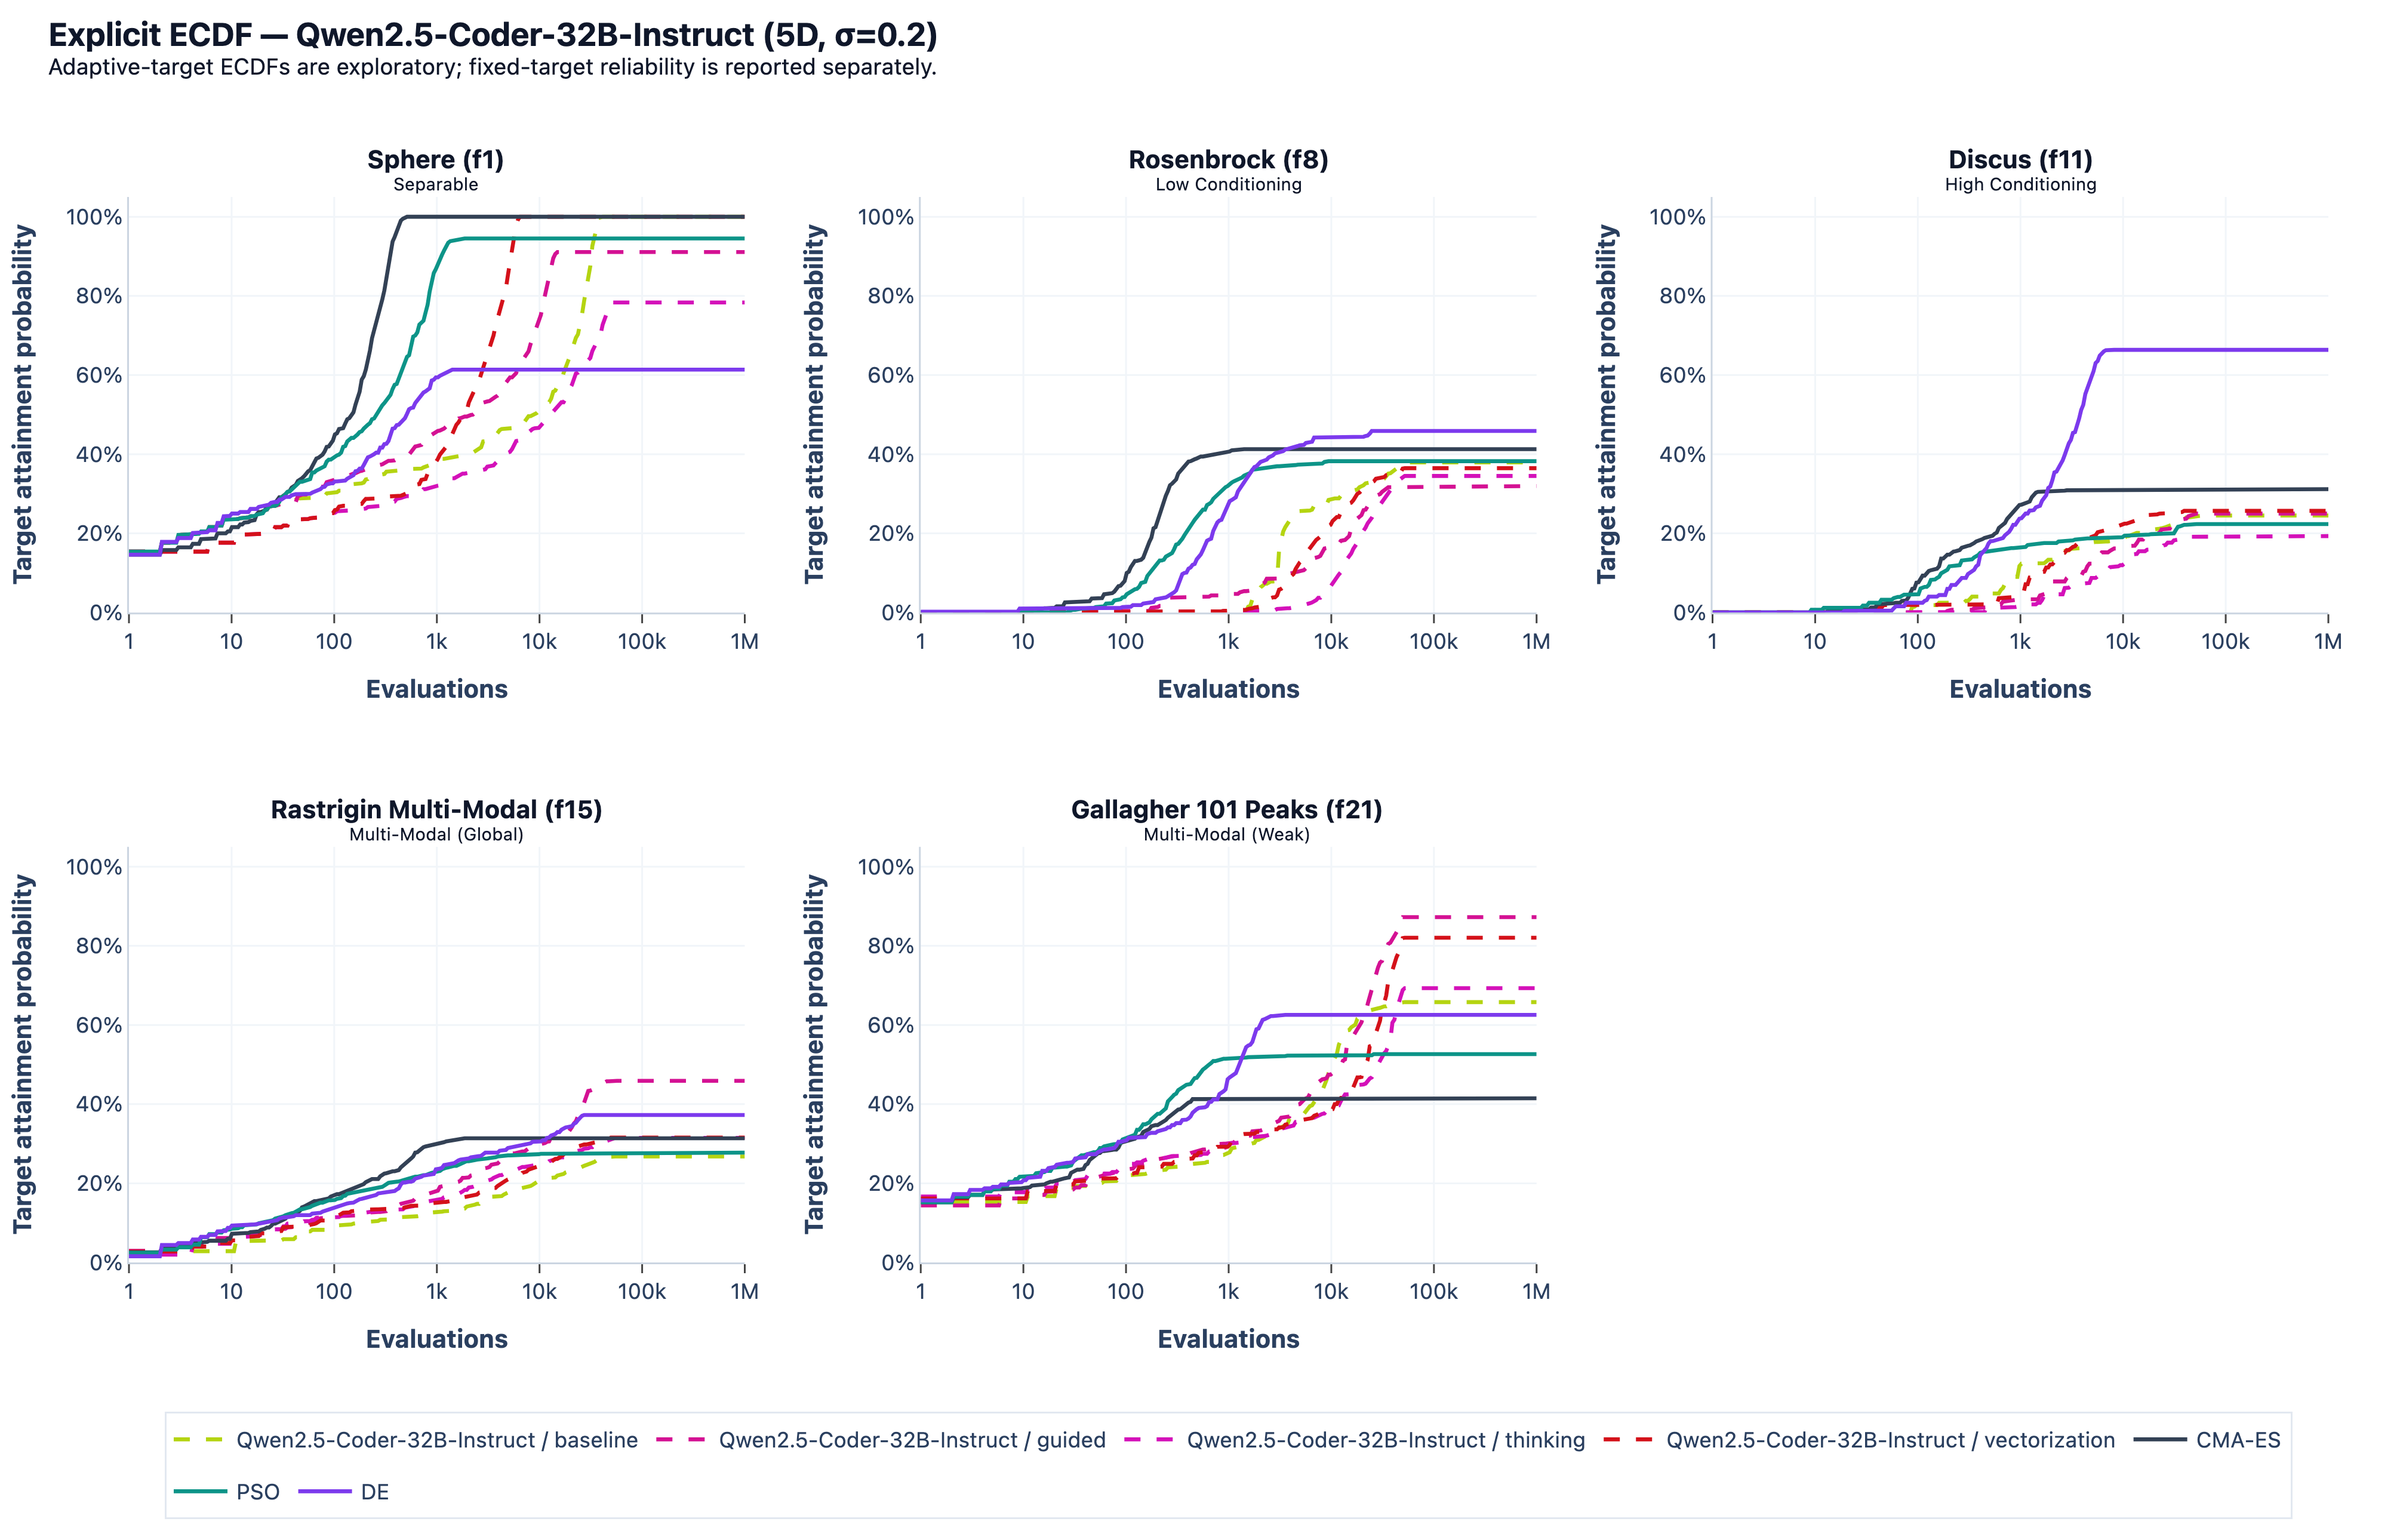
\includegraphics[width=\textwidth,height=0.32\textheight,keepaspectratio]{images/experiments/02_explicit/qwen_32b/5D/std_0.2/target_precision_ecdf.png}
    \caption{Qwen2.5-Coder-32B-Instruct: Explicit, $D=5$,
    $\sigma=0.2$. Convergence (median and IQR) above;
    adaptive target-precision ECDF below. The objective-query allowance
    is 50,000.}
    \label{fig:appendix_02_explicit_qwen_32b_5_std_02}
\end{minipage}
\par\medskip

\subsection{DeepSeek-Coder-V2-Lite-Instruct}
\nopagebreak[4]

\par\smallskip\noindent
\begin{minipage}{\linewidth}
    \captionsetup{type=figure,aboveskip=4pt,belowskip=0pt}
    \centering
    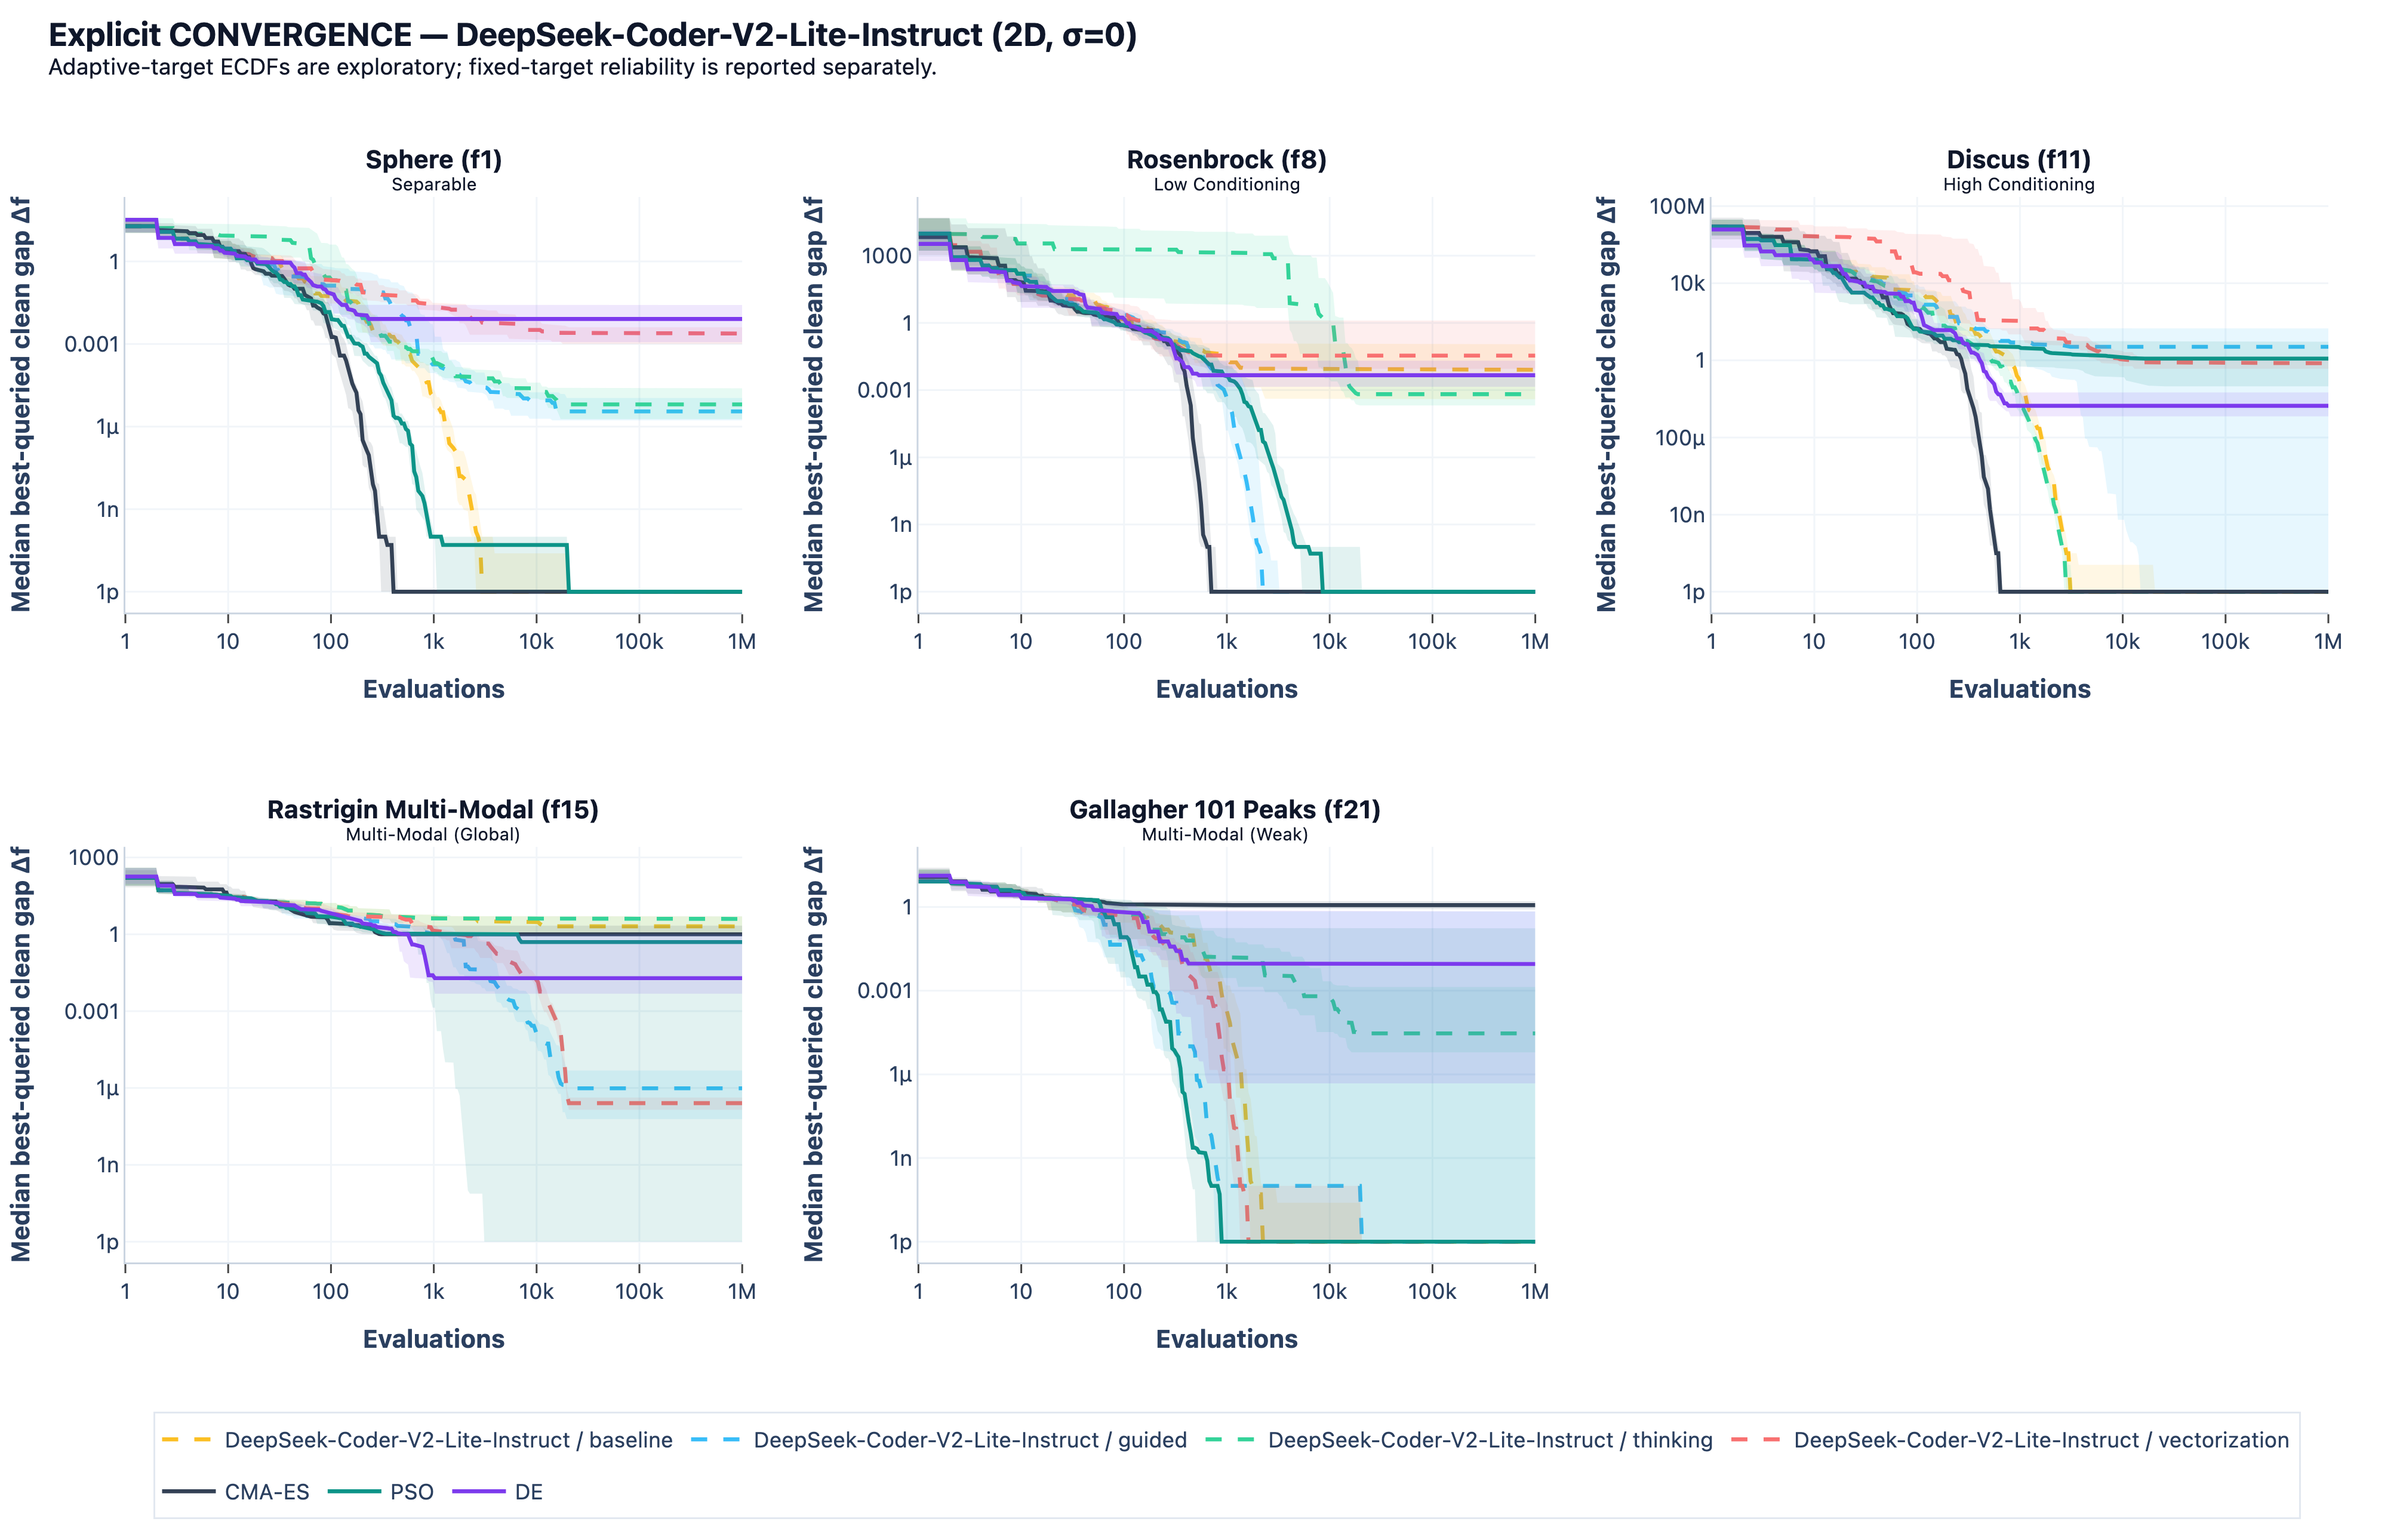
\includegraphics[width=\textwidth,height=0.32\textheight,keepaspectratio]{images/experiments/02_explicit/deepseek_coder_v2_lite_instruct_q4_k_m/2D/std_0.0/convergence_trajectories.png}
    \par\medskip
    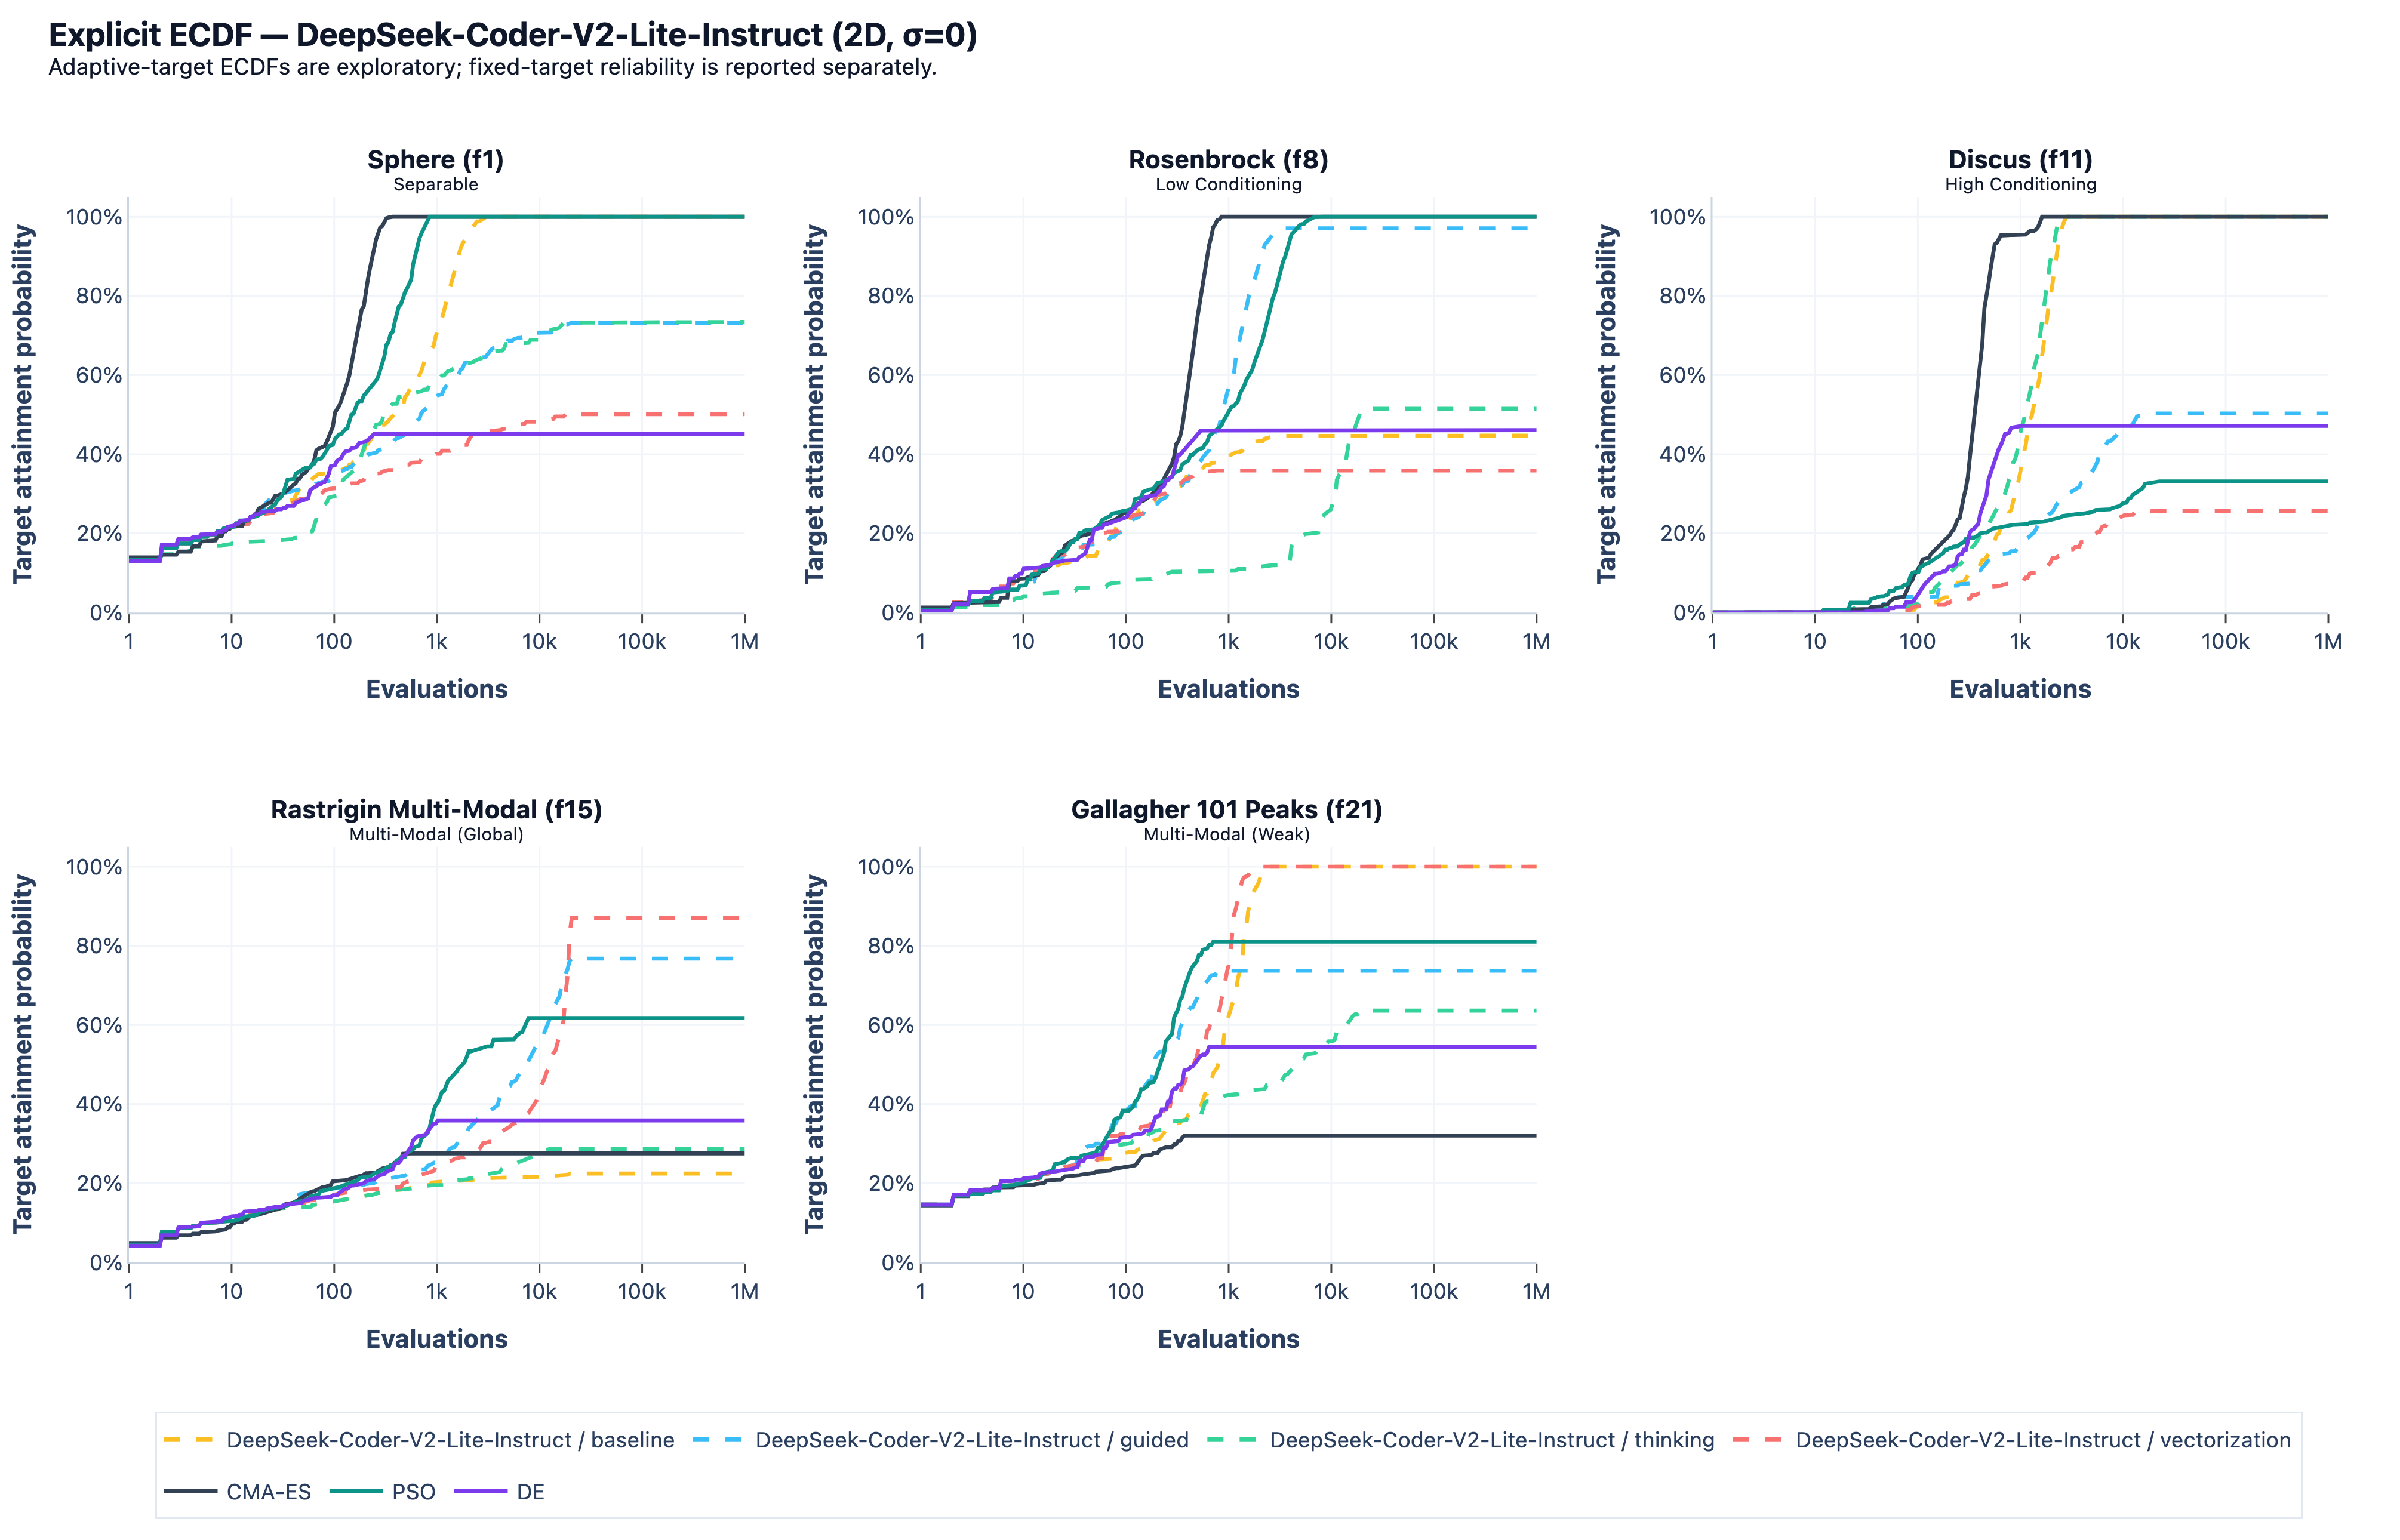
\includegraphics[width=\textwidth,height=0.32\textheight,keepaspectratio]{images/experiments/02_explicit/deepseek_coder_v2_lite_instruct_q4_k_m/2D/std_0.0/target_precision_ecdf.png}
    \caption{DeepSeek-Coder-V2-Lite-Instruct: Explicit, $D=2$,
    $\sigma=0.0$. Convergence (median and IQR) above;
    adaptive target-precision ECDF below. The objective-query allowance
    is 20,000.}
    \label{fig:appendix_02_explicit_deepseek_coder_v2_lite_instruct_q4_k_m_2_std_00}
\end{minipage}
\par\medskip

\par\smallskip\noindent
\begin{minipage}{\linewidth}
    \captionsetup{type=figure,aboveskip=4pt,belowskip=0pt}
    \centering
    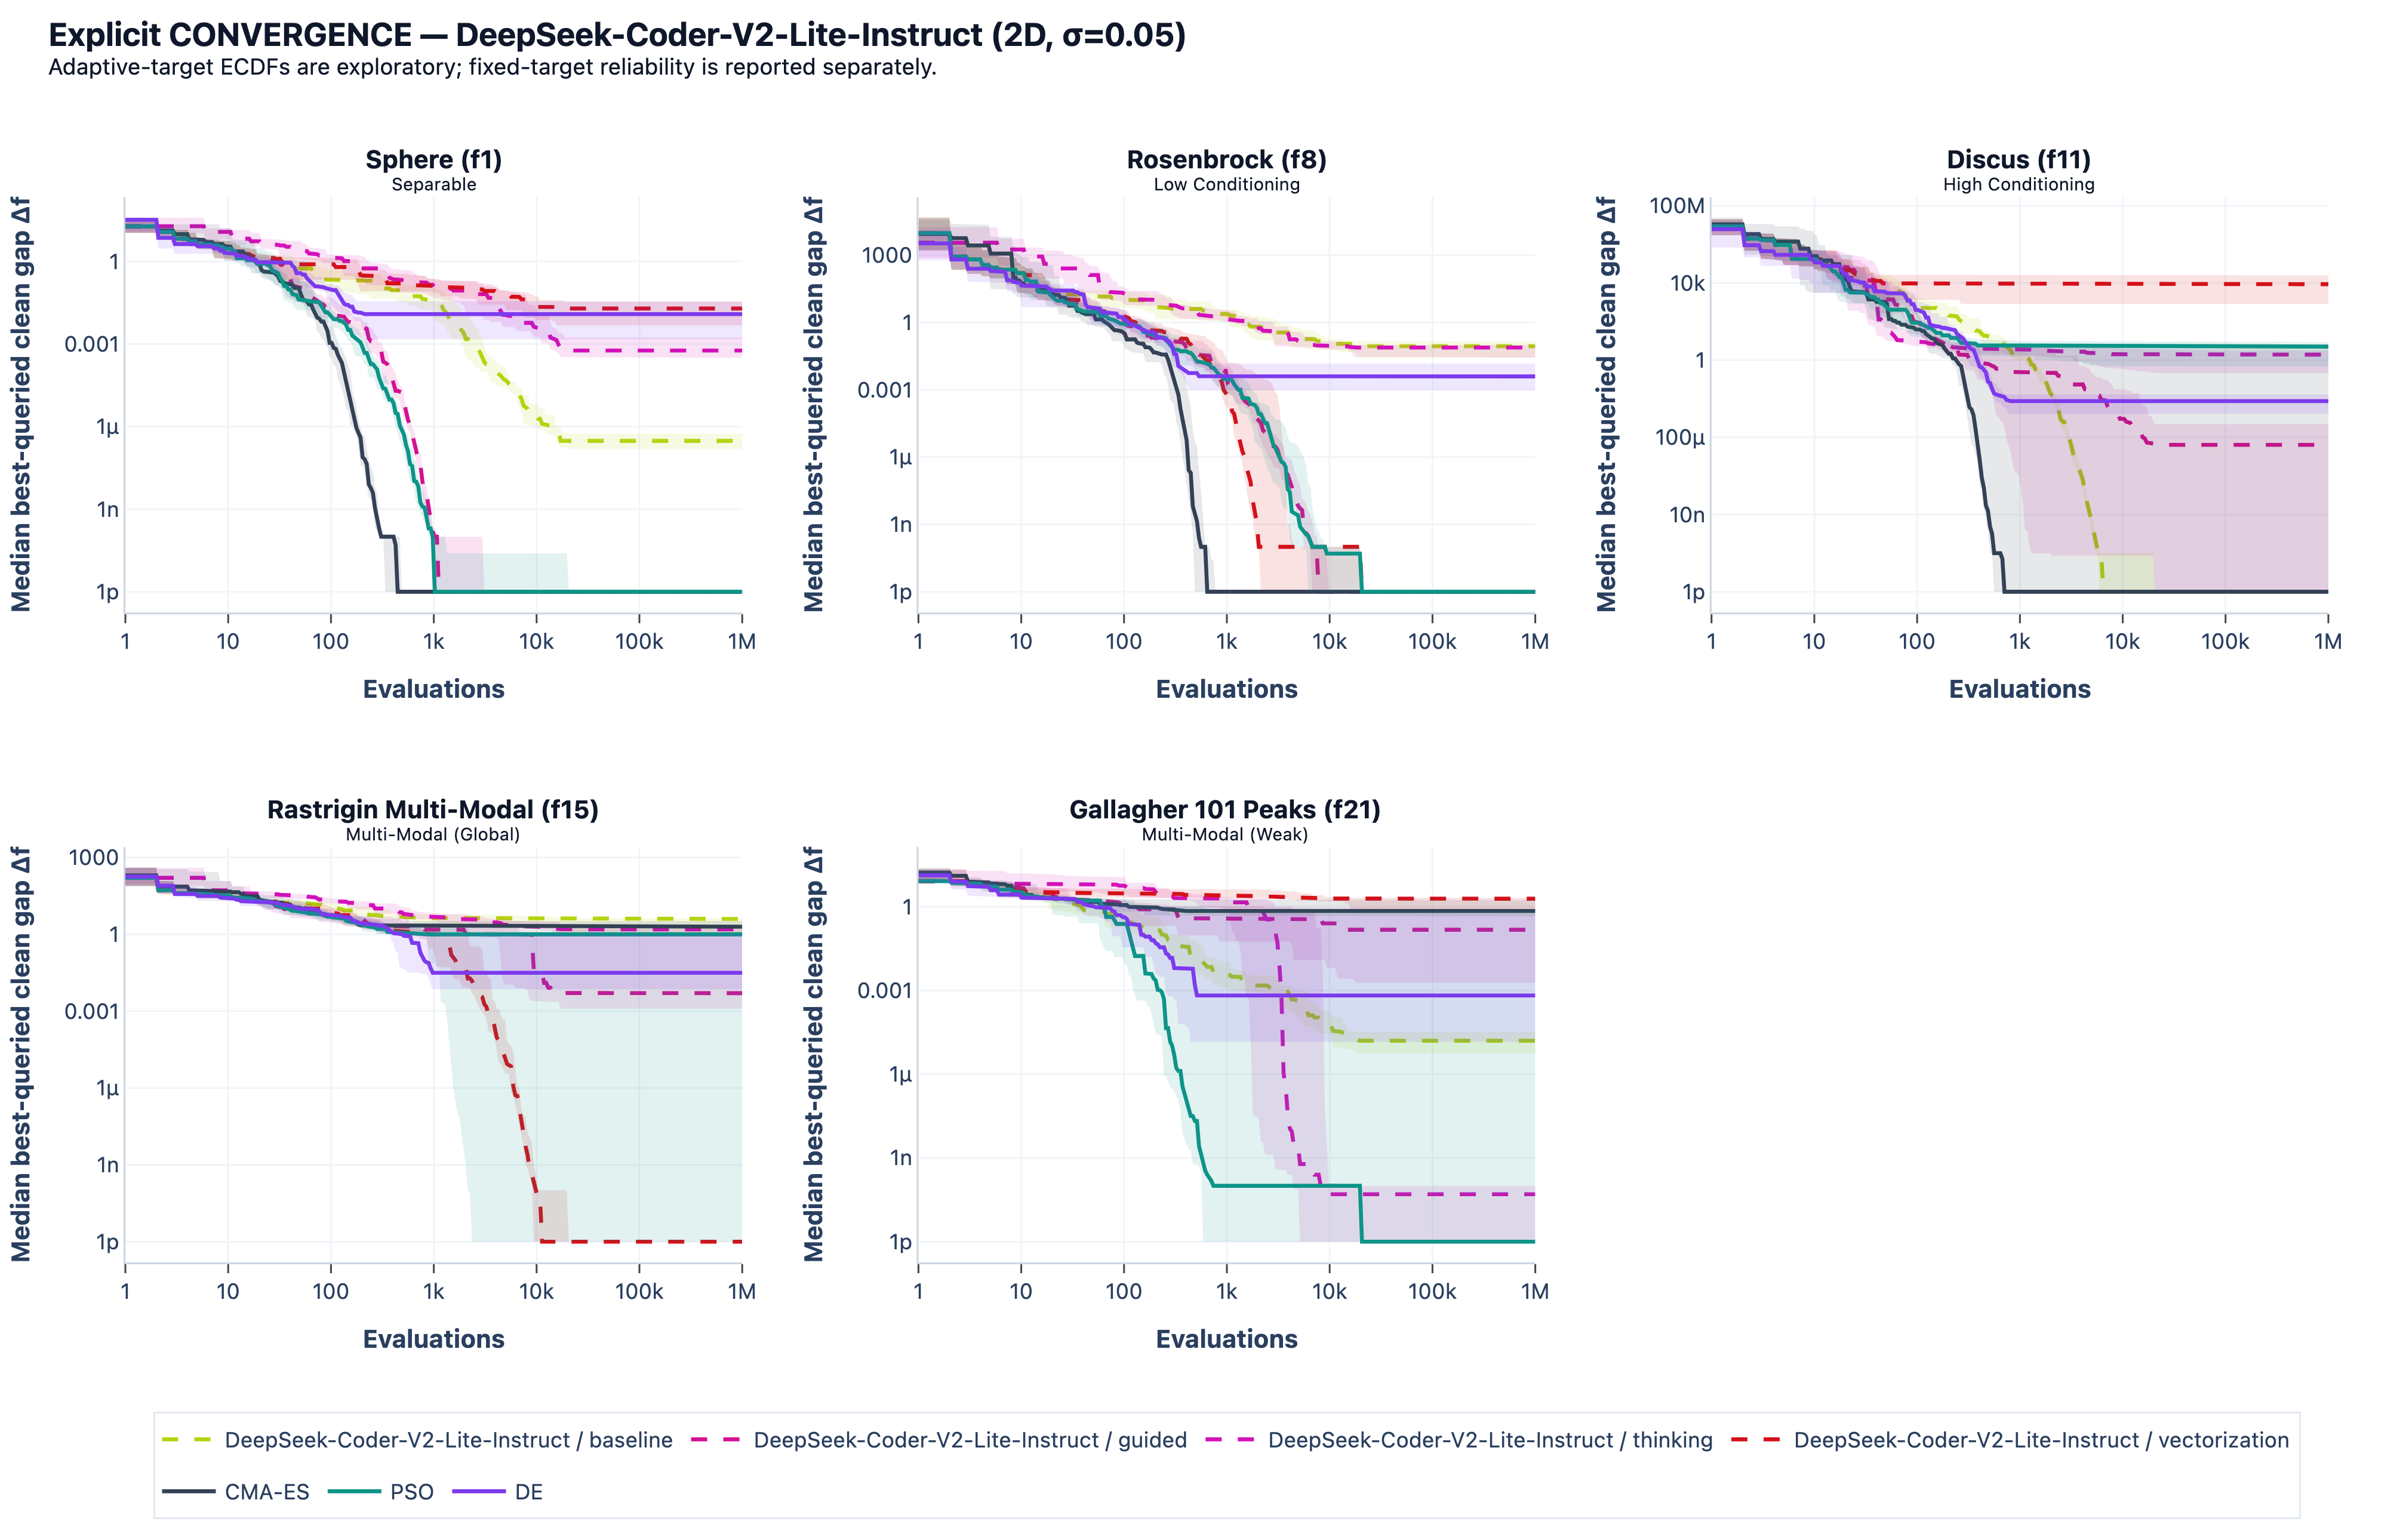
\includegraphics[width=\textwidth,height=0.32\textheight,keepaspectratio]{images/experiments/02_explicit/deepseek_coder_v2_lite_instruct_q4_k_m/2D/std_0.05/convergence_trajectories.png}
    \par\medskip
    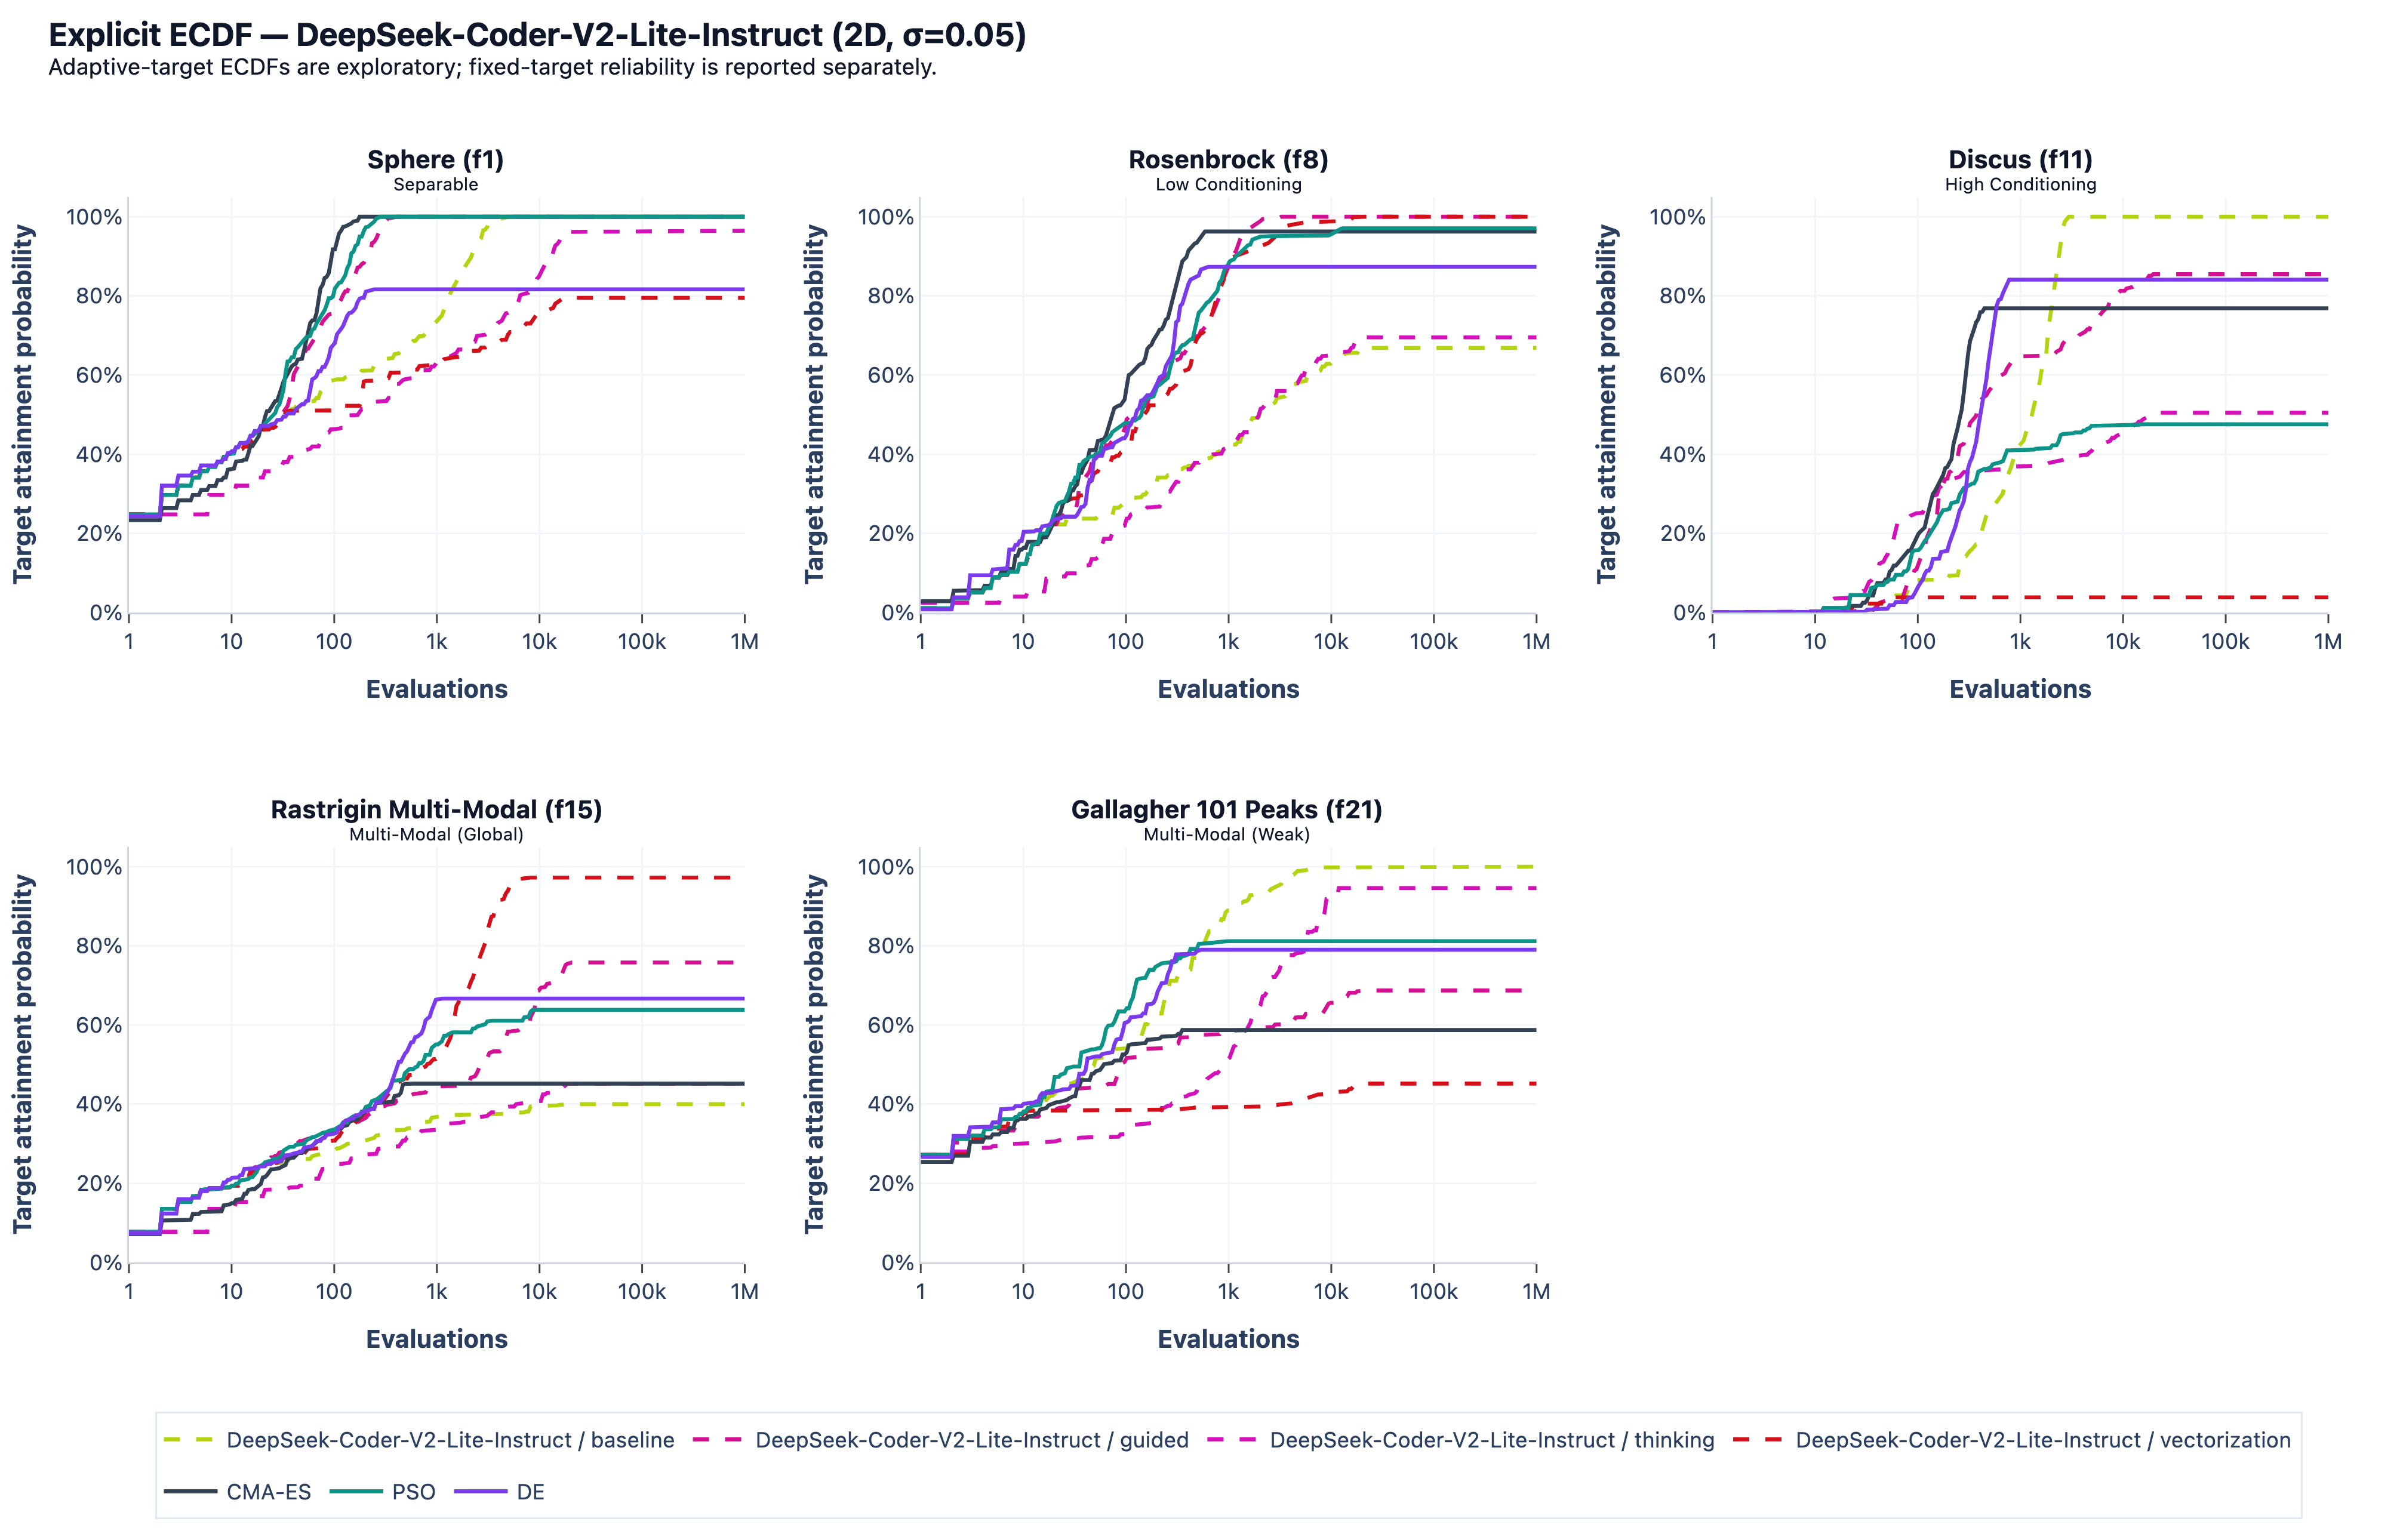
\includegraphics[width=\textwidth,height=0.32\textheight,keepaspectratio]{images/experiments/02_explicit/deepseek_coder_v2_lite_instruct_q4_k_m/2D/std_0.05/target_precision_ecdf.png}
    \caption{DeepSeek-Coder-V2-Lite-Instruct: Explicit, $D=2$,
    $\sigma=0.05$. Convergence (median and IQR) above;
    adaptive target-precision ECDF below. The objective-query allowance
    is 20,000.}
    \label{fig:appendix_02_explicit_deepseek_coder_v2_lite_instruct_q4_k_m_2_std_005}
\end{minipage}
\par\medskip

\par\smallskip\noindent
\begin{minipage}{\linewidth}
    \captionsetup{type=figure,aboveskip=4pt,belowskip=0pt}
    \centering
    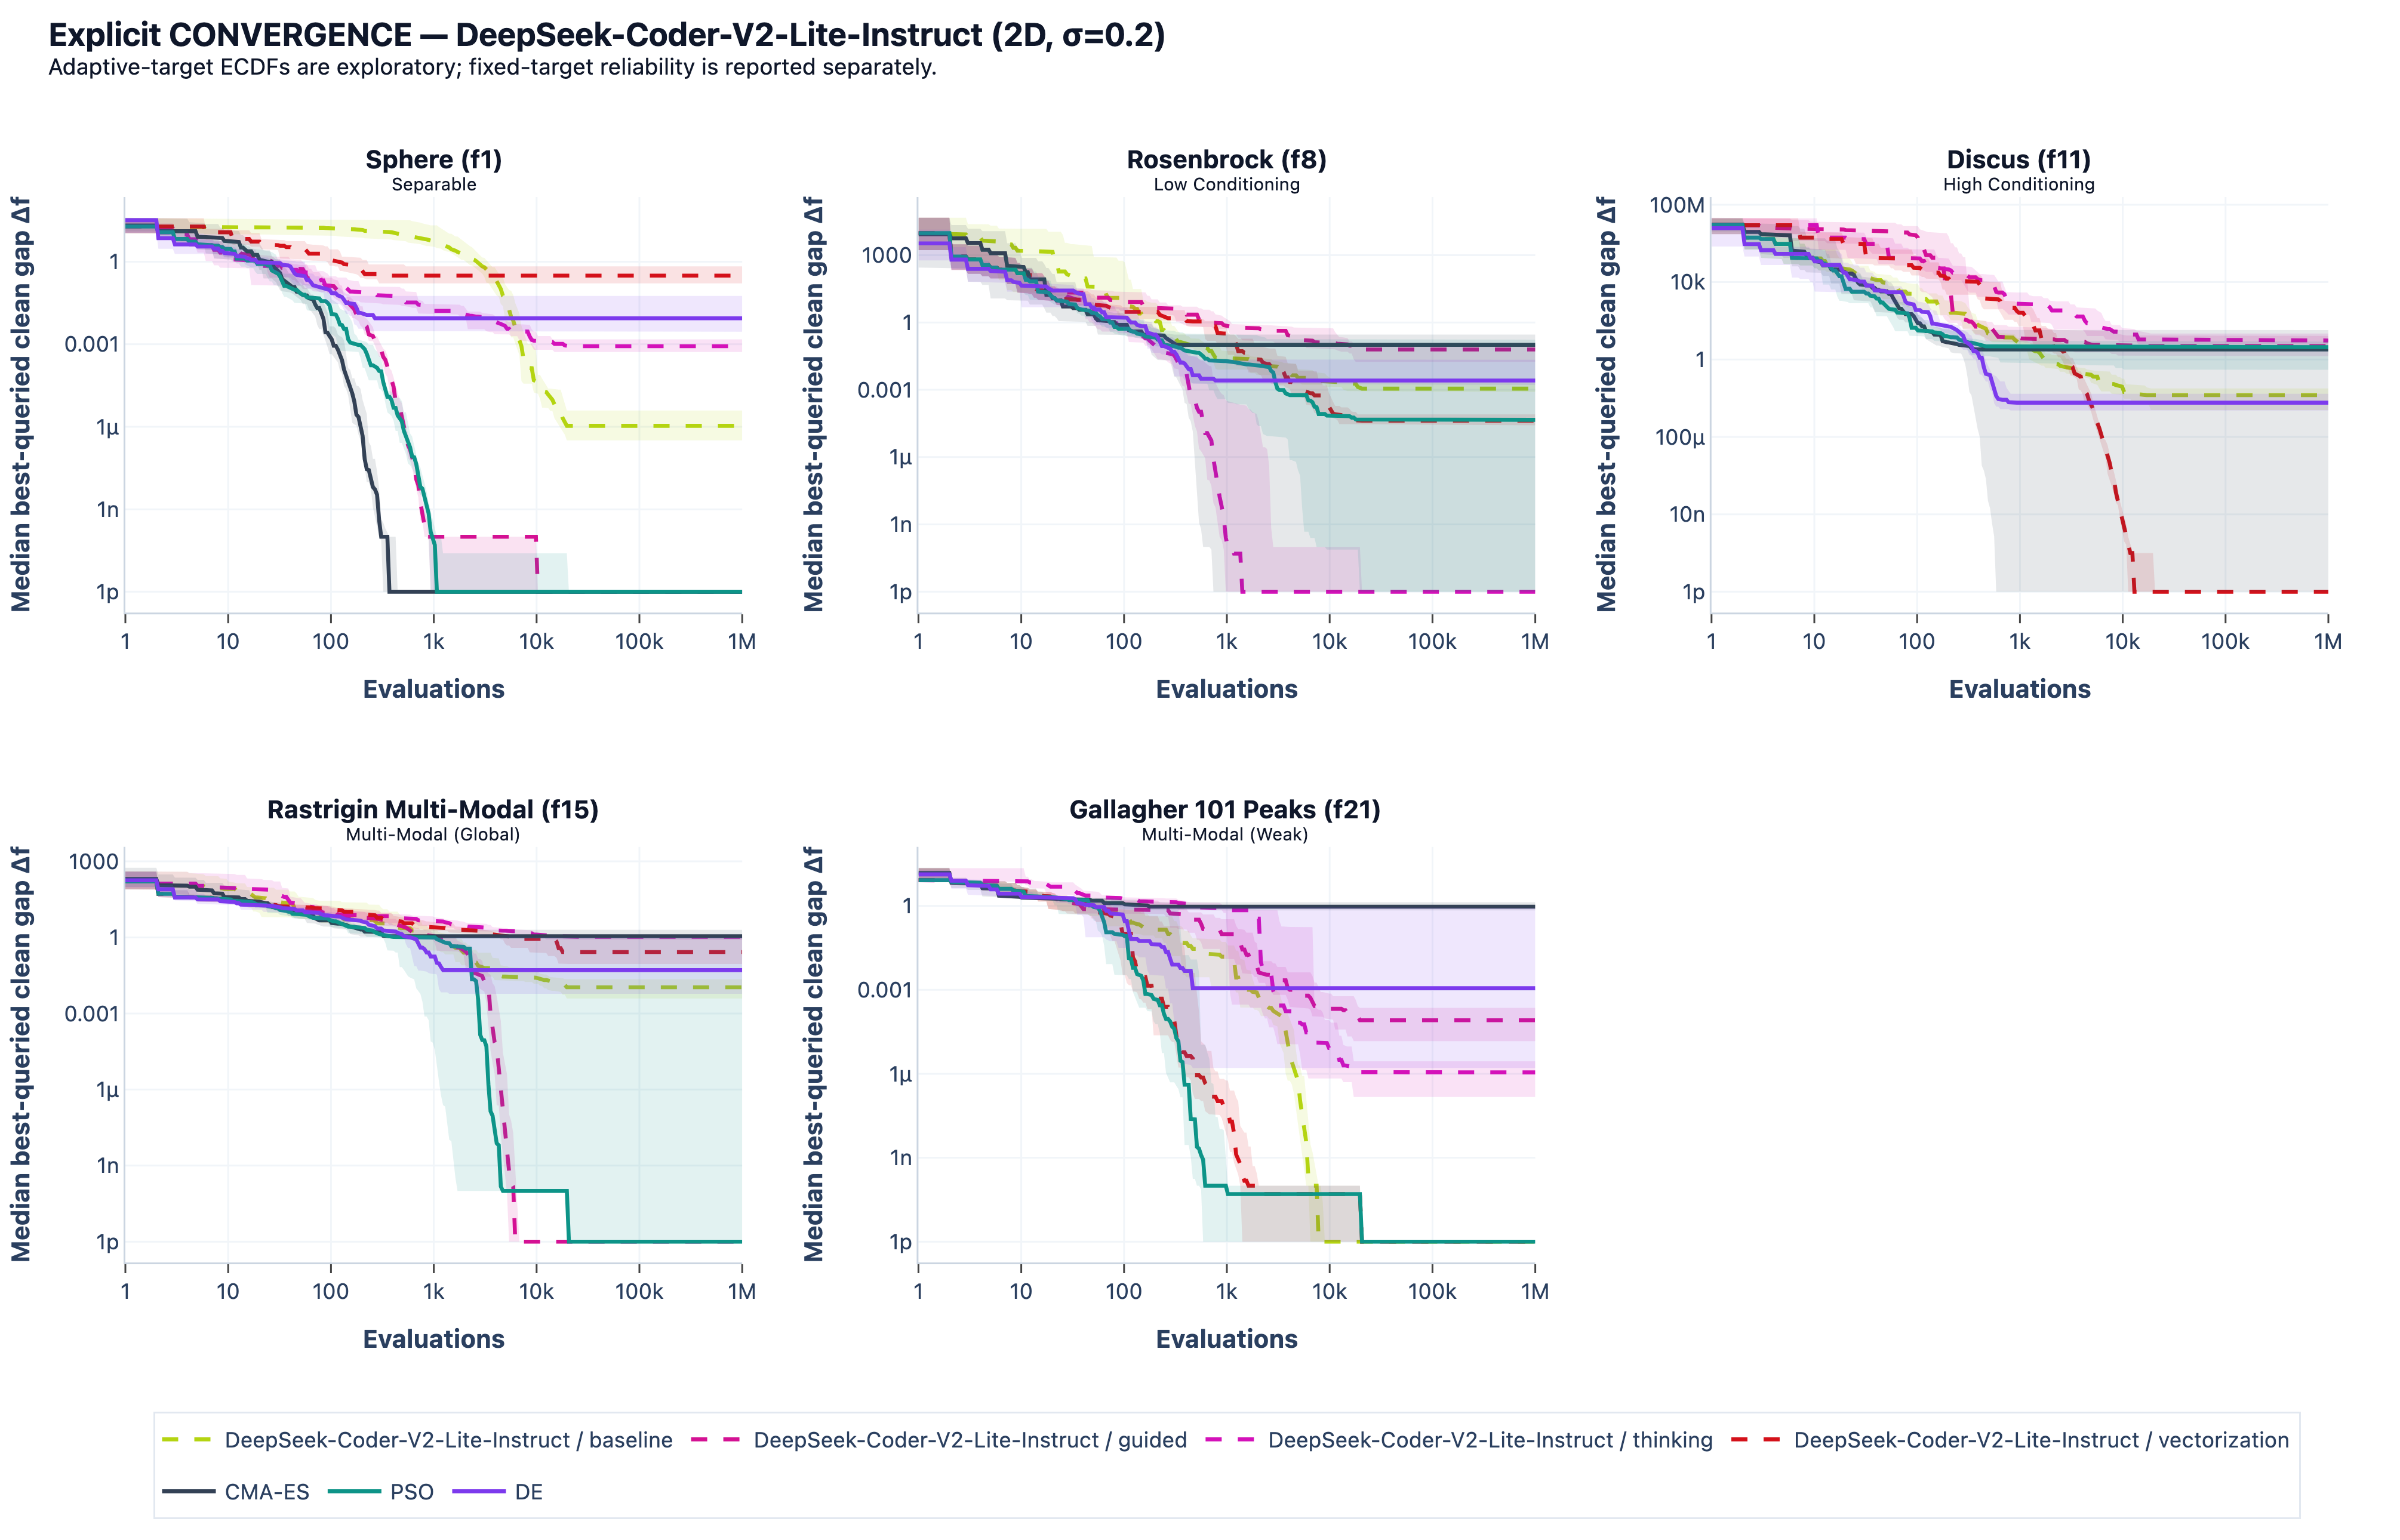
\includegraphics[width=\textwidth,height=0.32\textheight,keepaspectratio]{images/experiments/02_explicit/deepseek_coder_v2_lite_instruct_q4_k_m/2D/std_0.2/convergence_trajectories.png}
    \par\medskip
    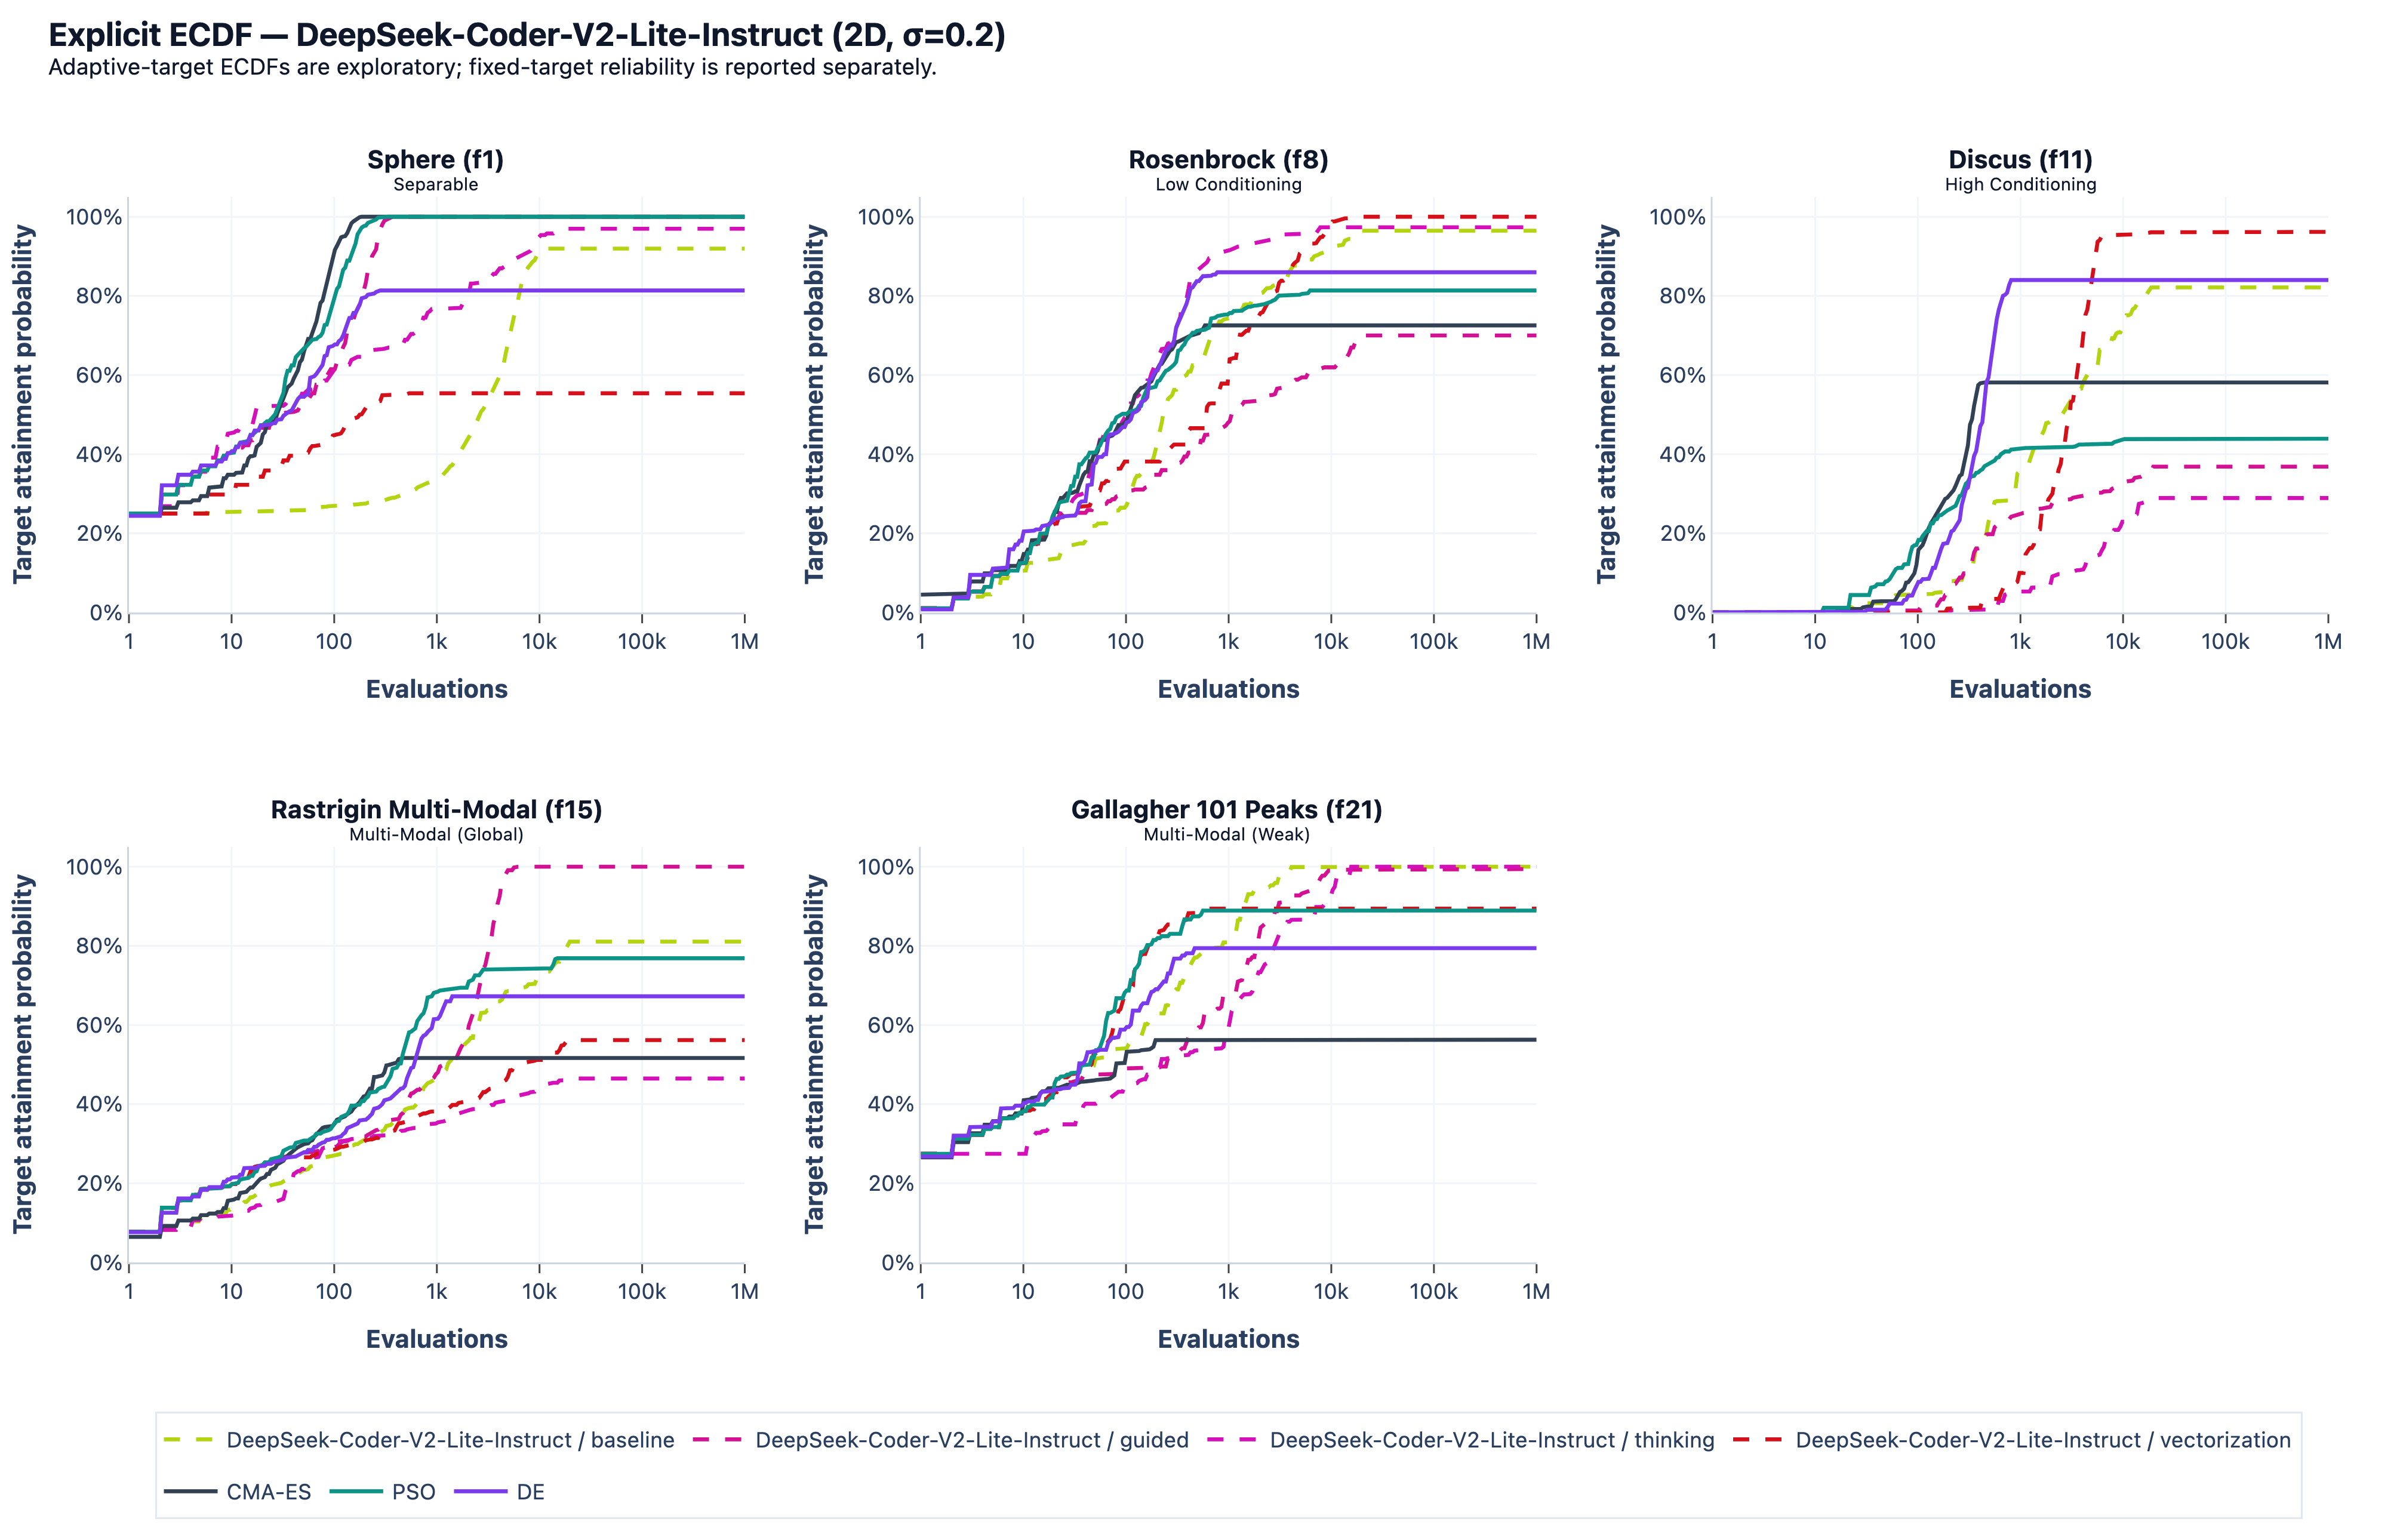
\includegraphics[width=\textwidth,height=0.32\textheight,keepaspectratio]{images/experiments/02_explicit/deepseek_coder_v2_lite_instruct_q4_k_m/2D/std_0.2/target_precision_ecdf.png}
    \caption{DeepSeek-Coder-V2-Lite-Instruct: Explicit, $D=2$,
    $\sigma=0.2$. Convergence (median and IQR) above;
    adaptive target-precision ECDF below. The objective-query allowance
    is 20,000.}
    \label{fig:appendix_02_explicit_deepseek_coder_v2_lite_instruct_q4_k_m_2_std_02}
\end{minipage}
\par\medskip

\par\smallskip\noindent
\begin{minipage}{\linewidth}
    \captionsetup{type=figure,aboveskip=4pt,belowskip=0pt}
    \centering
    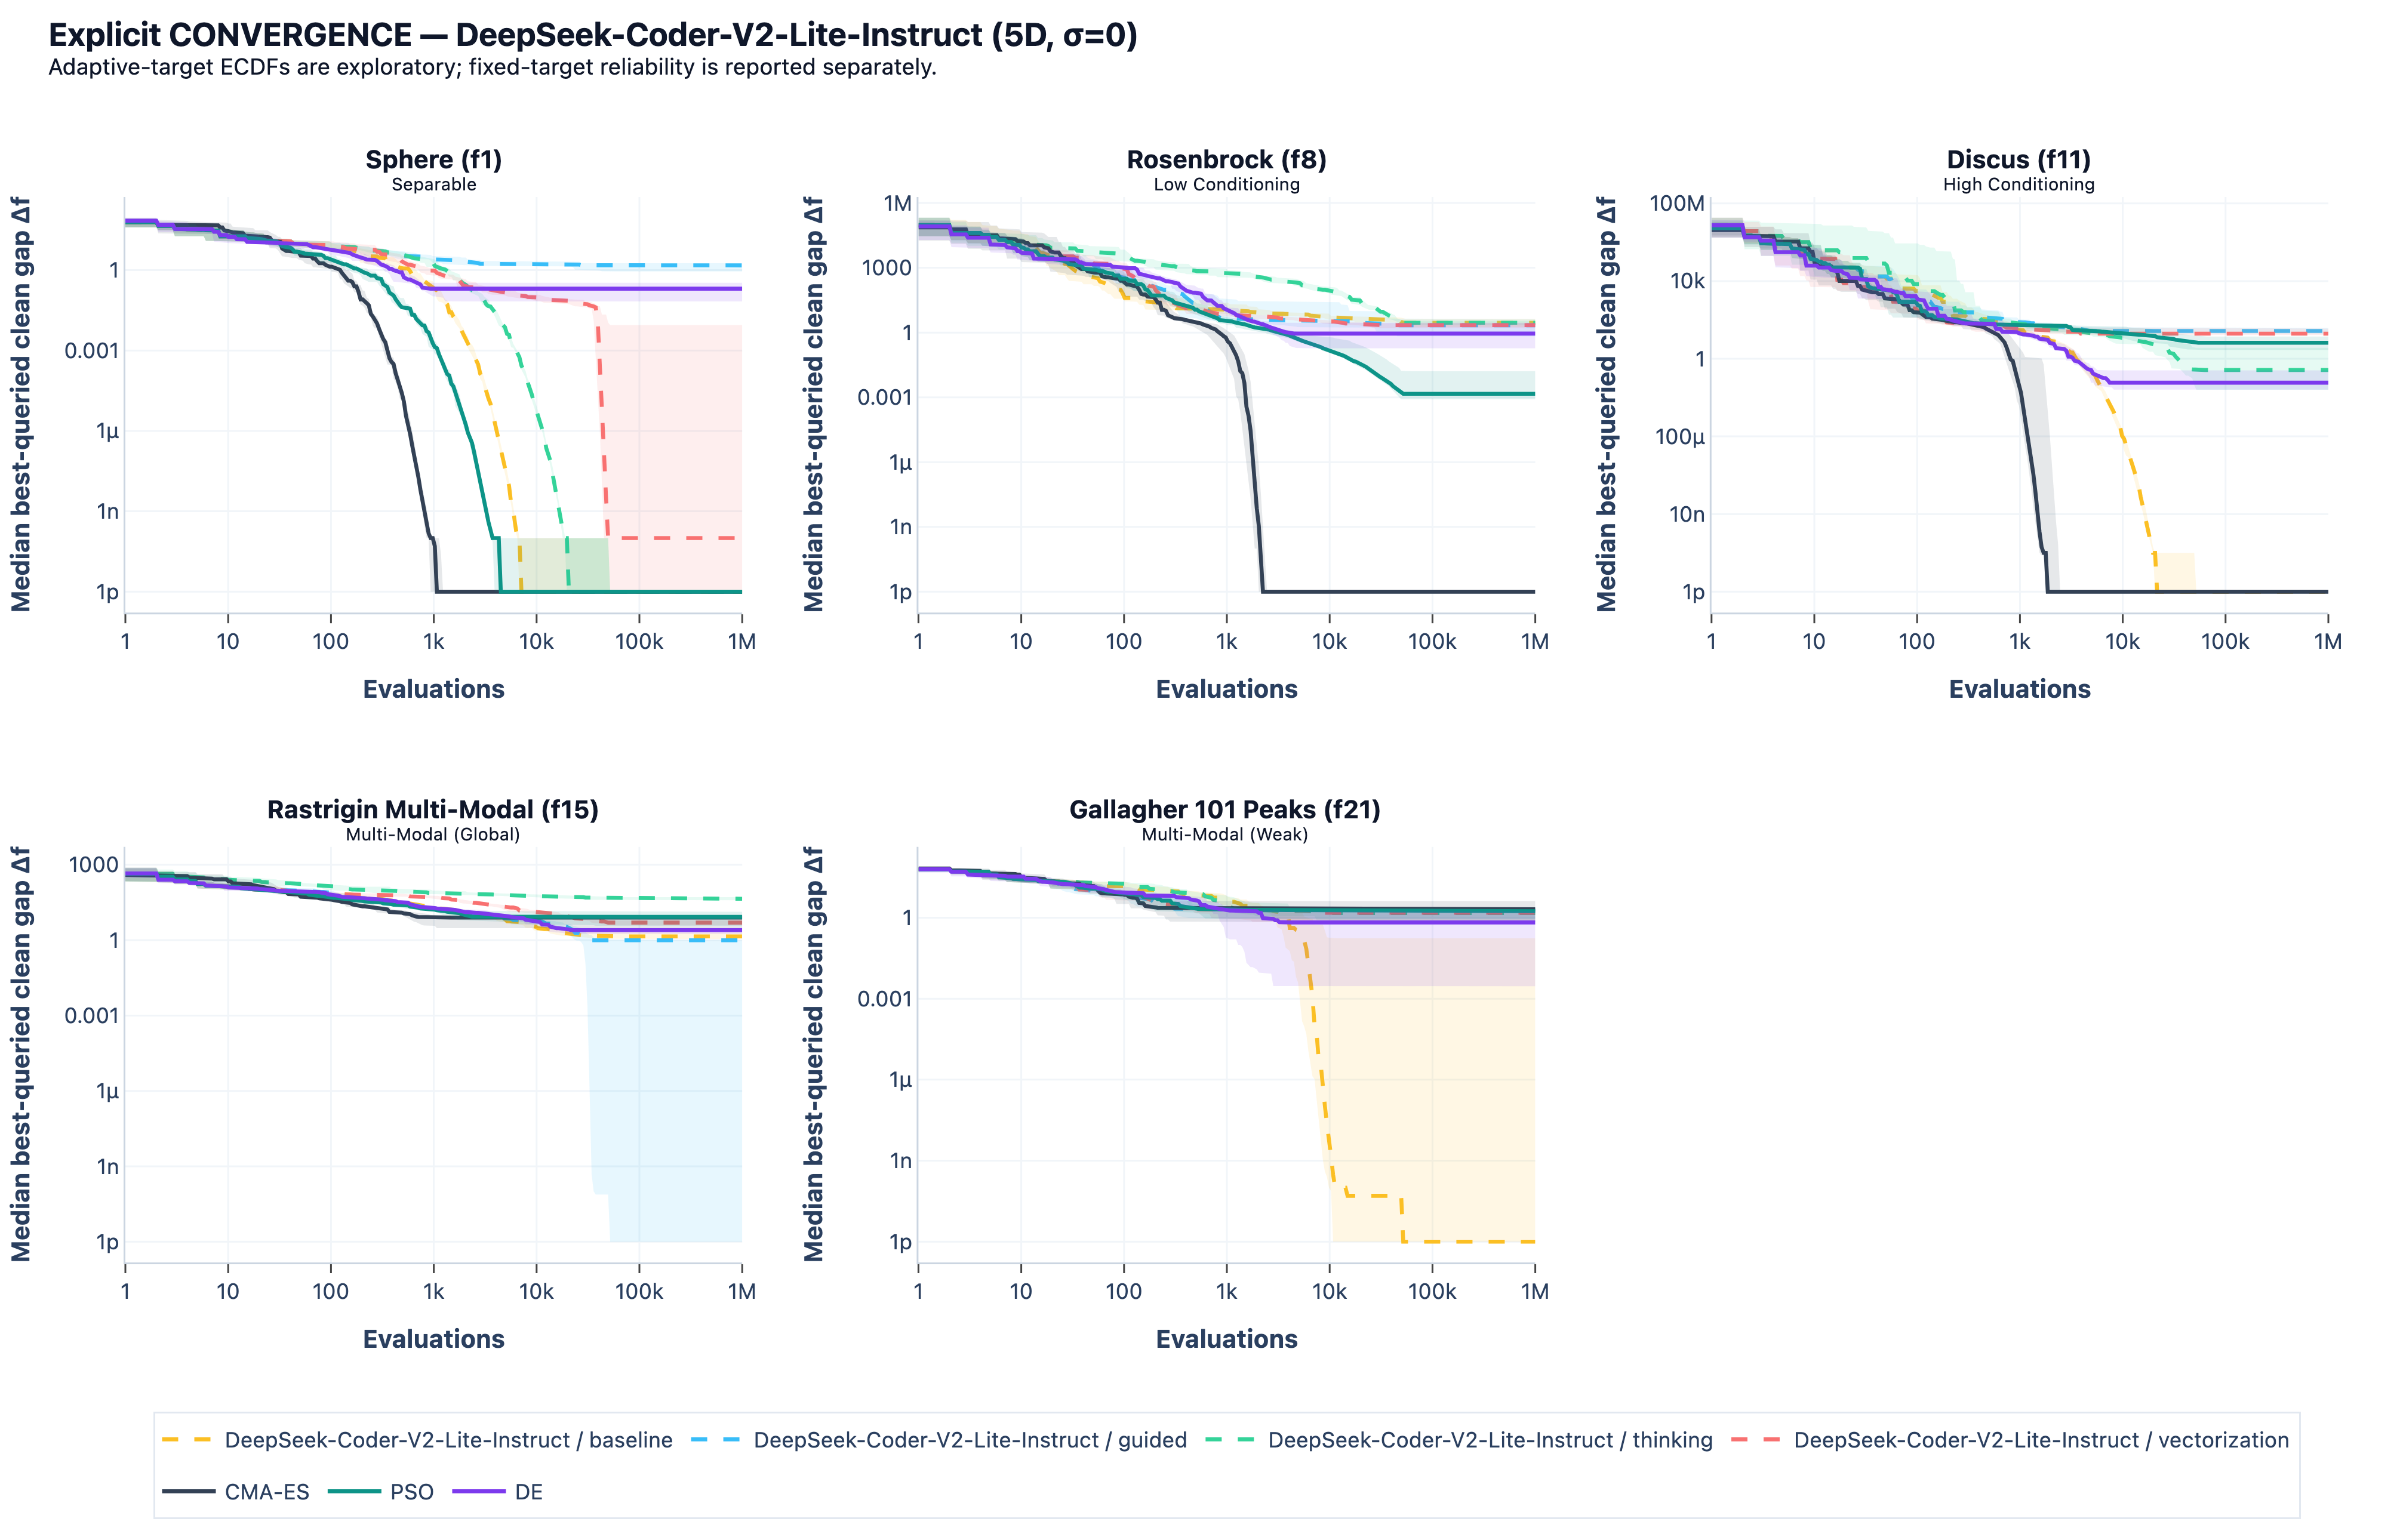
\includegraphics[width=\textwidth,height=0.32\textheight,keepaspectratio]{images/experiments/02_explicit/deepseek_coder_v2_lite_instruct_q4_k_m/5D/std_0.0/convergence_trajectories.png}
    \par\medskip
    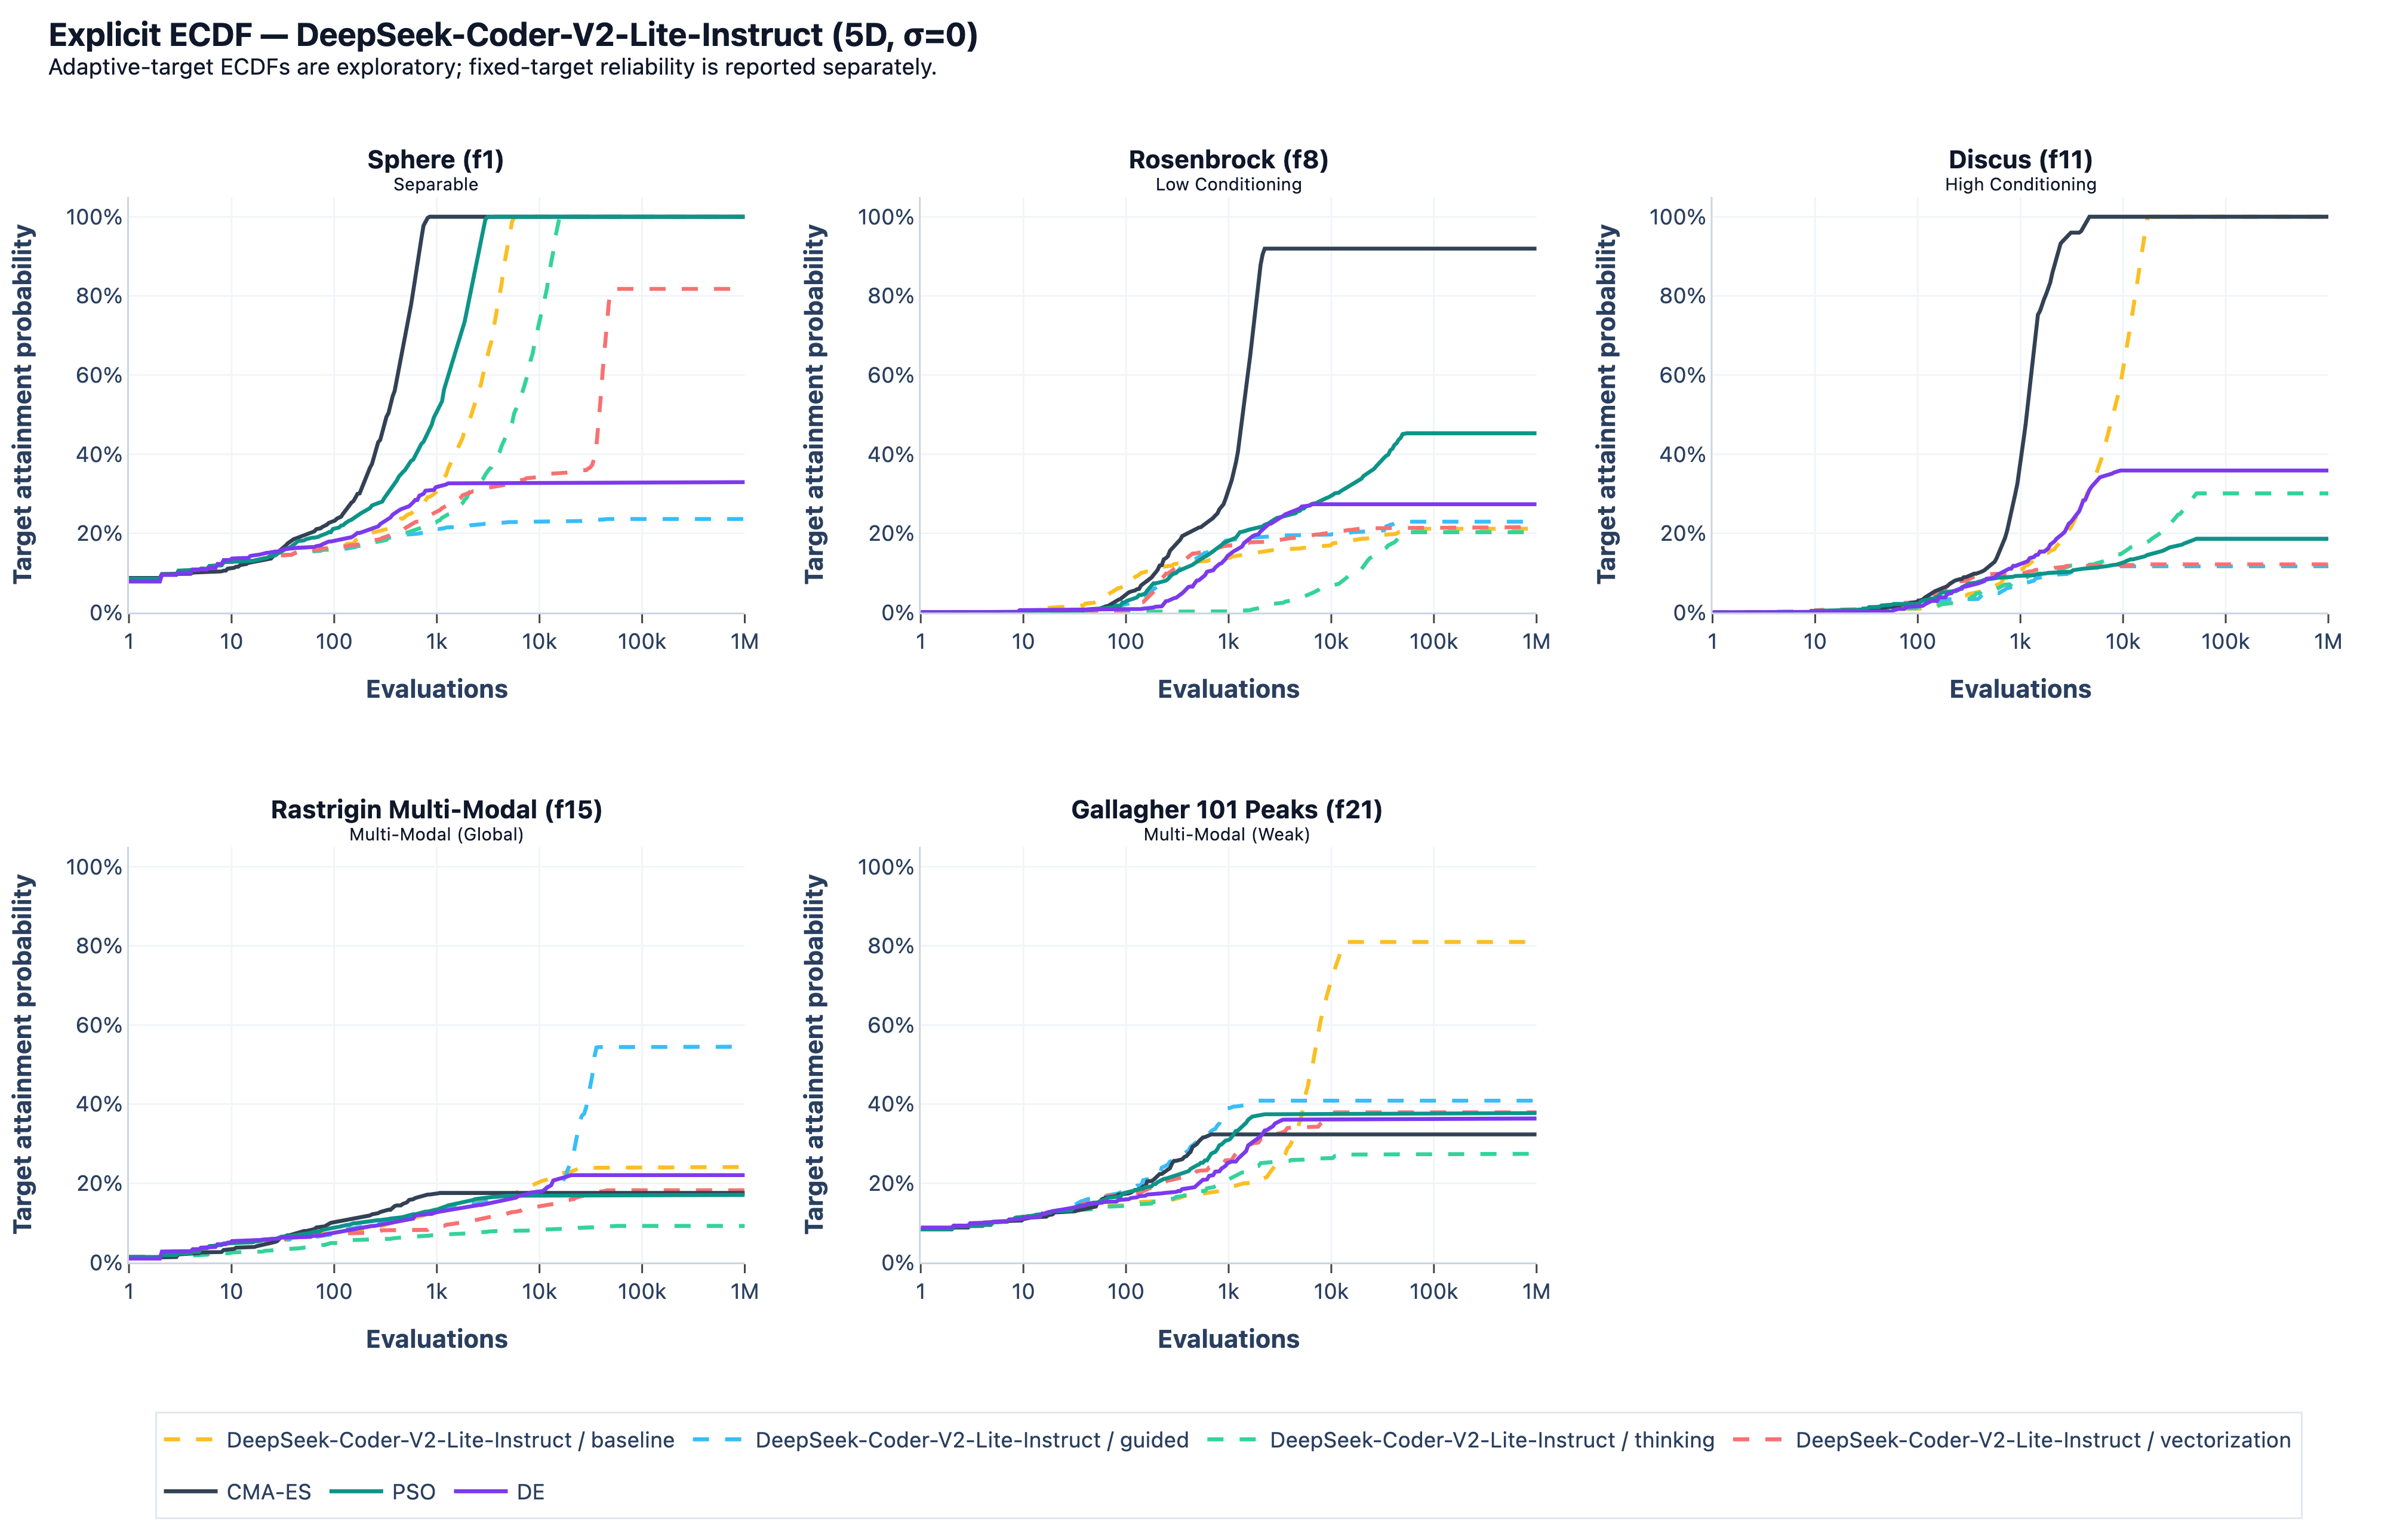
\includegraphics[width=\textwidth,height=0.32\textheight,keepaspectratio]{images/experiments/02_explicit/deepseek_coder_v2_lite_instruct_q4_k_m/5D/std_0.0/target_precision_ecdf.png}
    \caption{DeepSeek-Coder-V2-Lite-Instruct: Explicit, $D=5$,
    $\sigma=0.0$. Convergence (median and IQR) above;
    adaptive target-precision ECDF below. The objective-query allowance
    is 50,000.}
    \label{fig:appendix_02_explicit_deepseek_coder_v2_lite_instruct_q4_k_m_5_std_00}
\end{minipage}
\par\medskip

\par\smallskip\noindent
\begin{minipage}{\linewidth}
    \captionsetup{type=figure,aboveskip=4pt,belowskip=0pt}
    \centering
    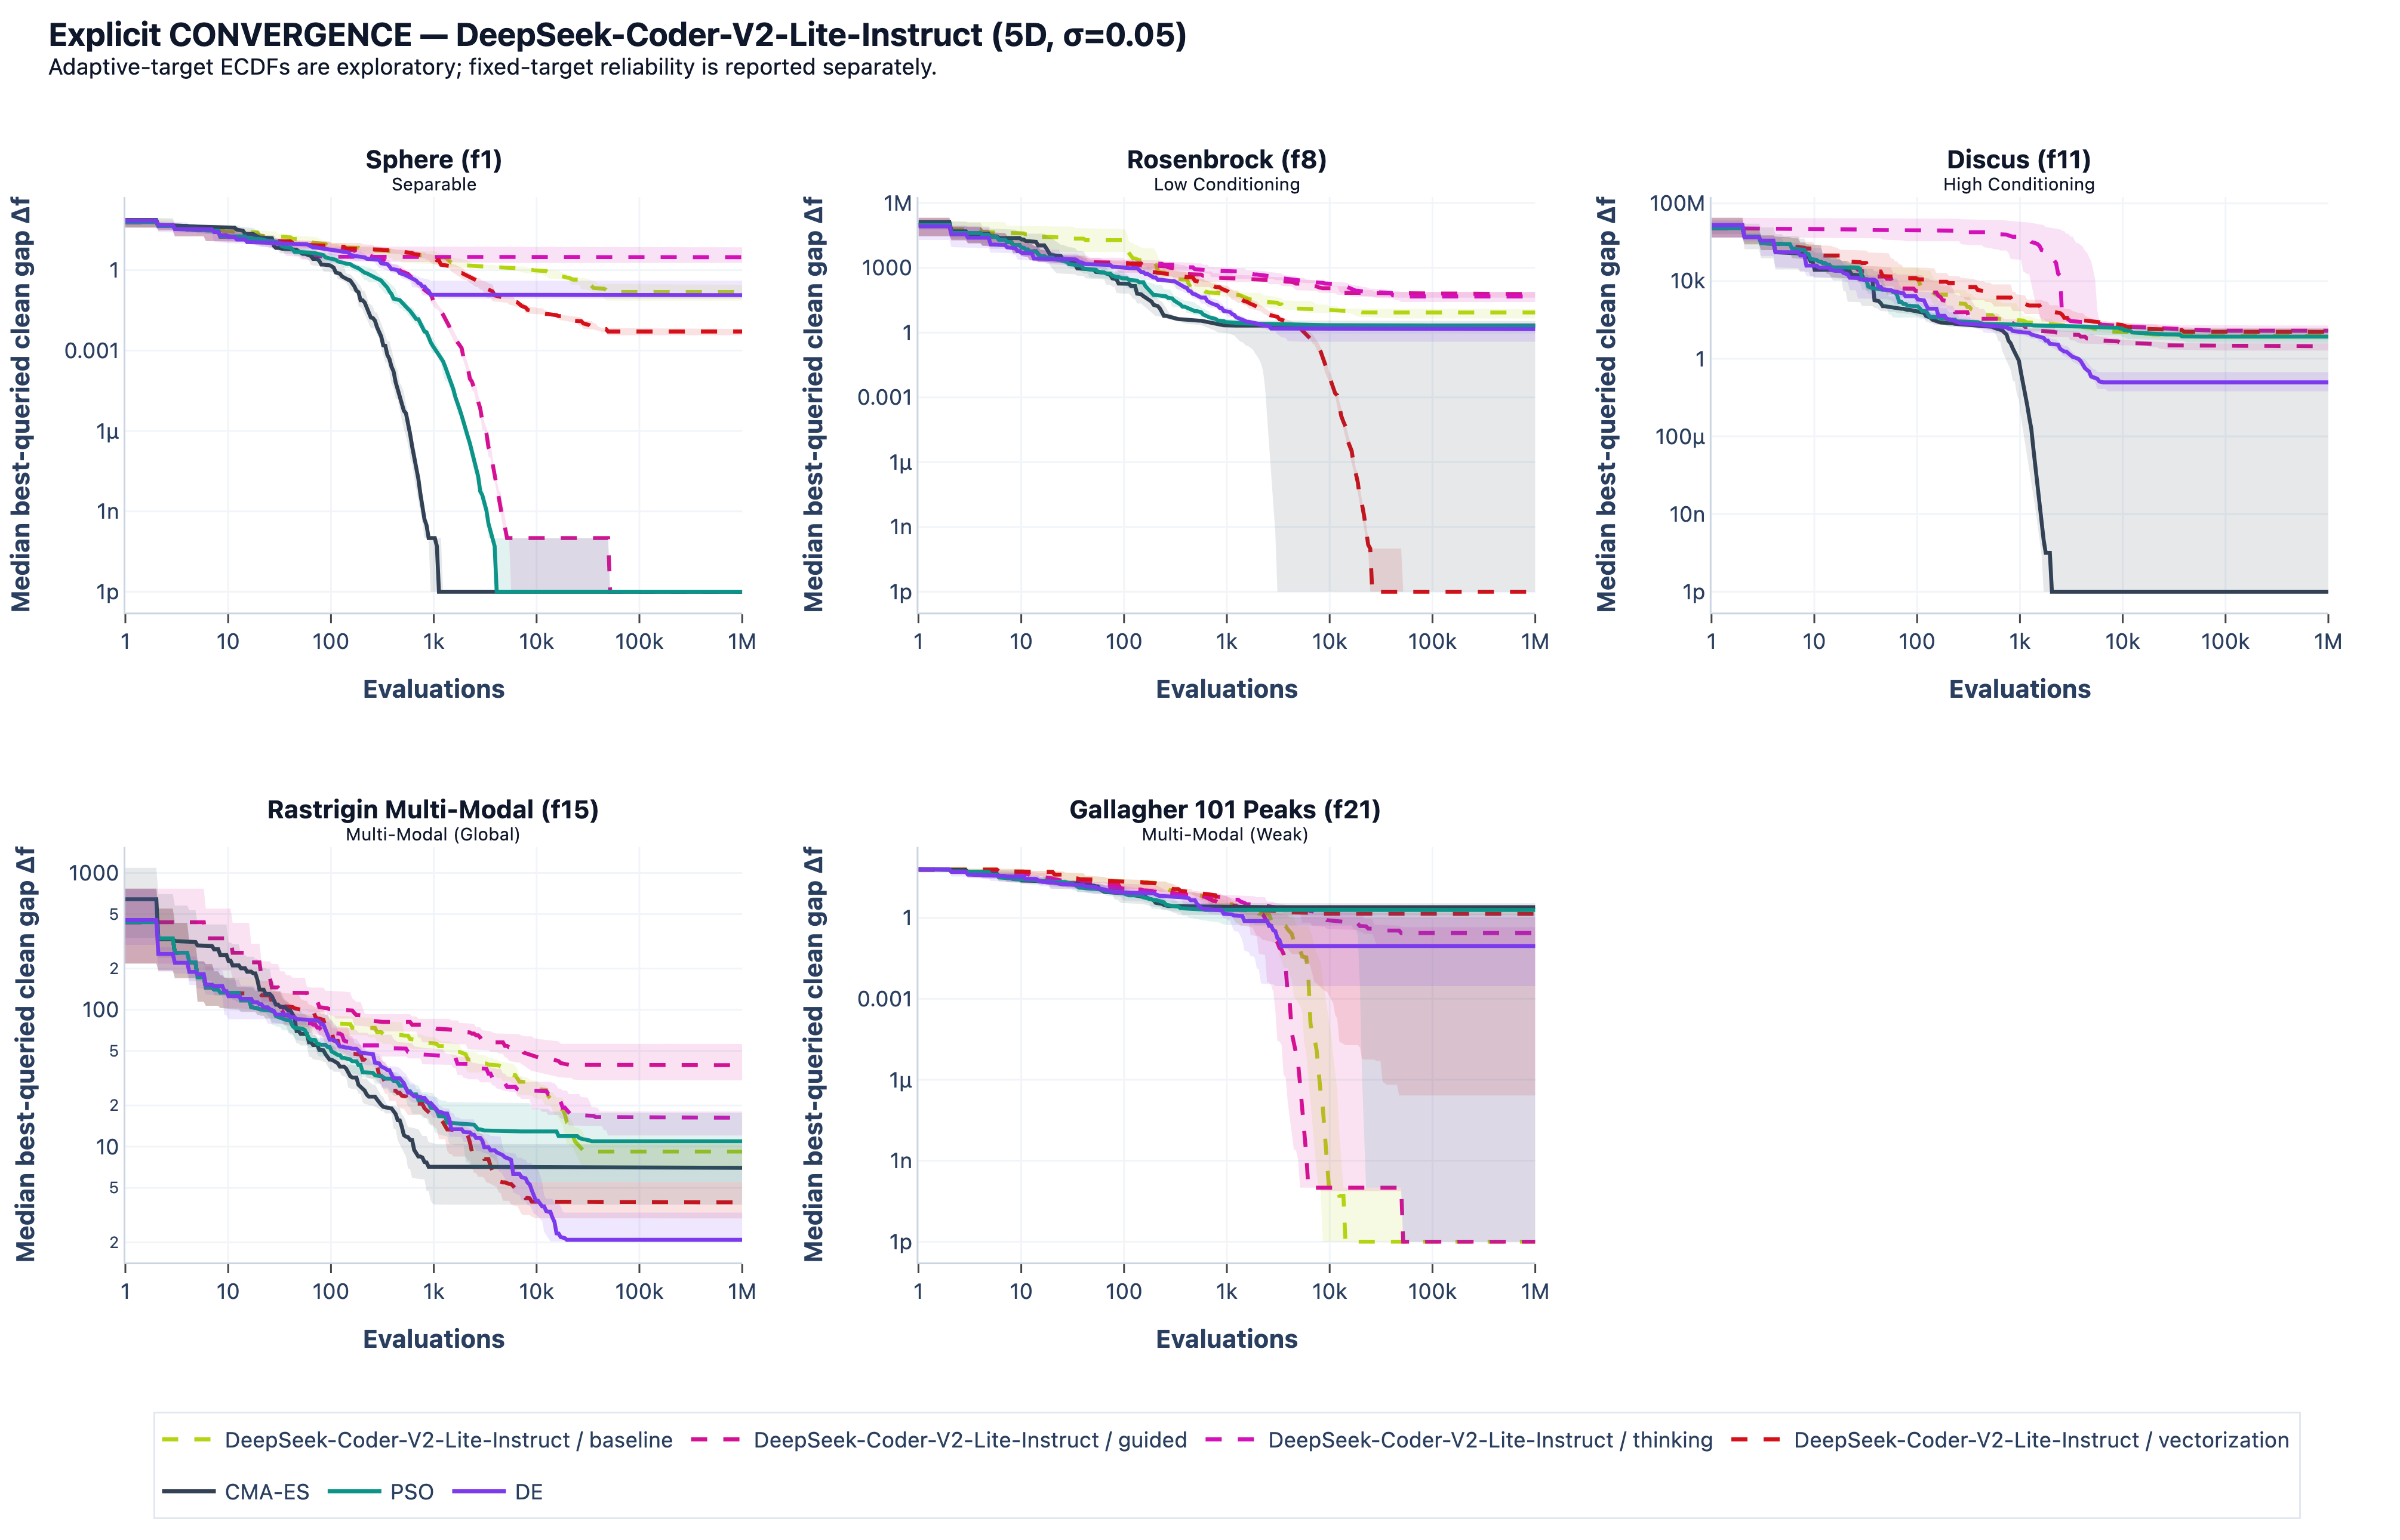
\includegraphics[width=\textwidth,height=0.32\textheight,keepaspectratio]{images/experiments/02_explicit/deepseek_coder_v2_lite_instruct_q4_k_m/5D/std_0.05/convergence_trajectories.png}
    \par\medskip
    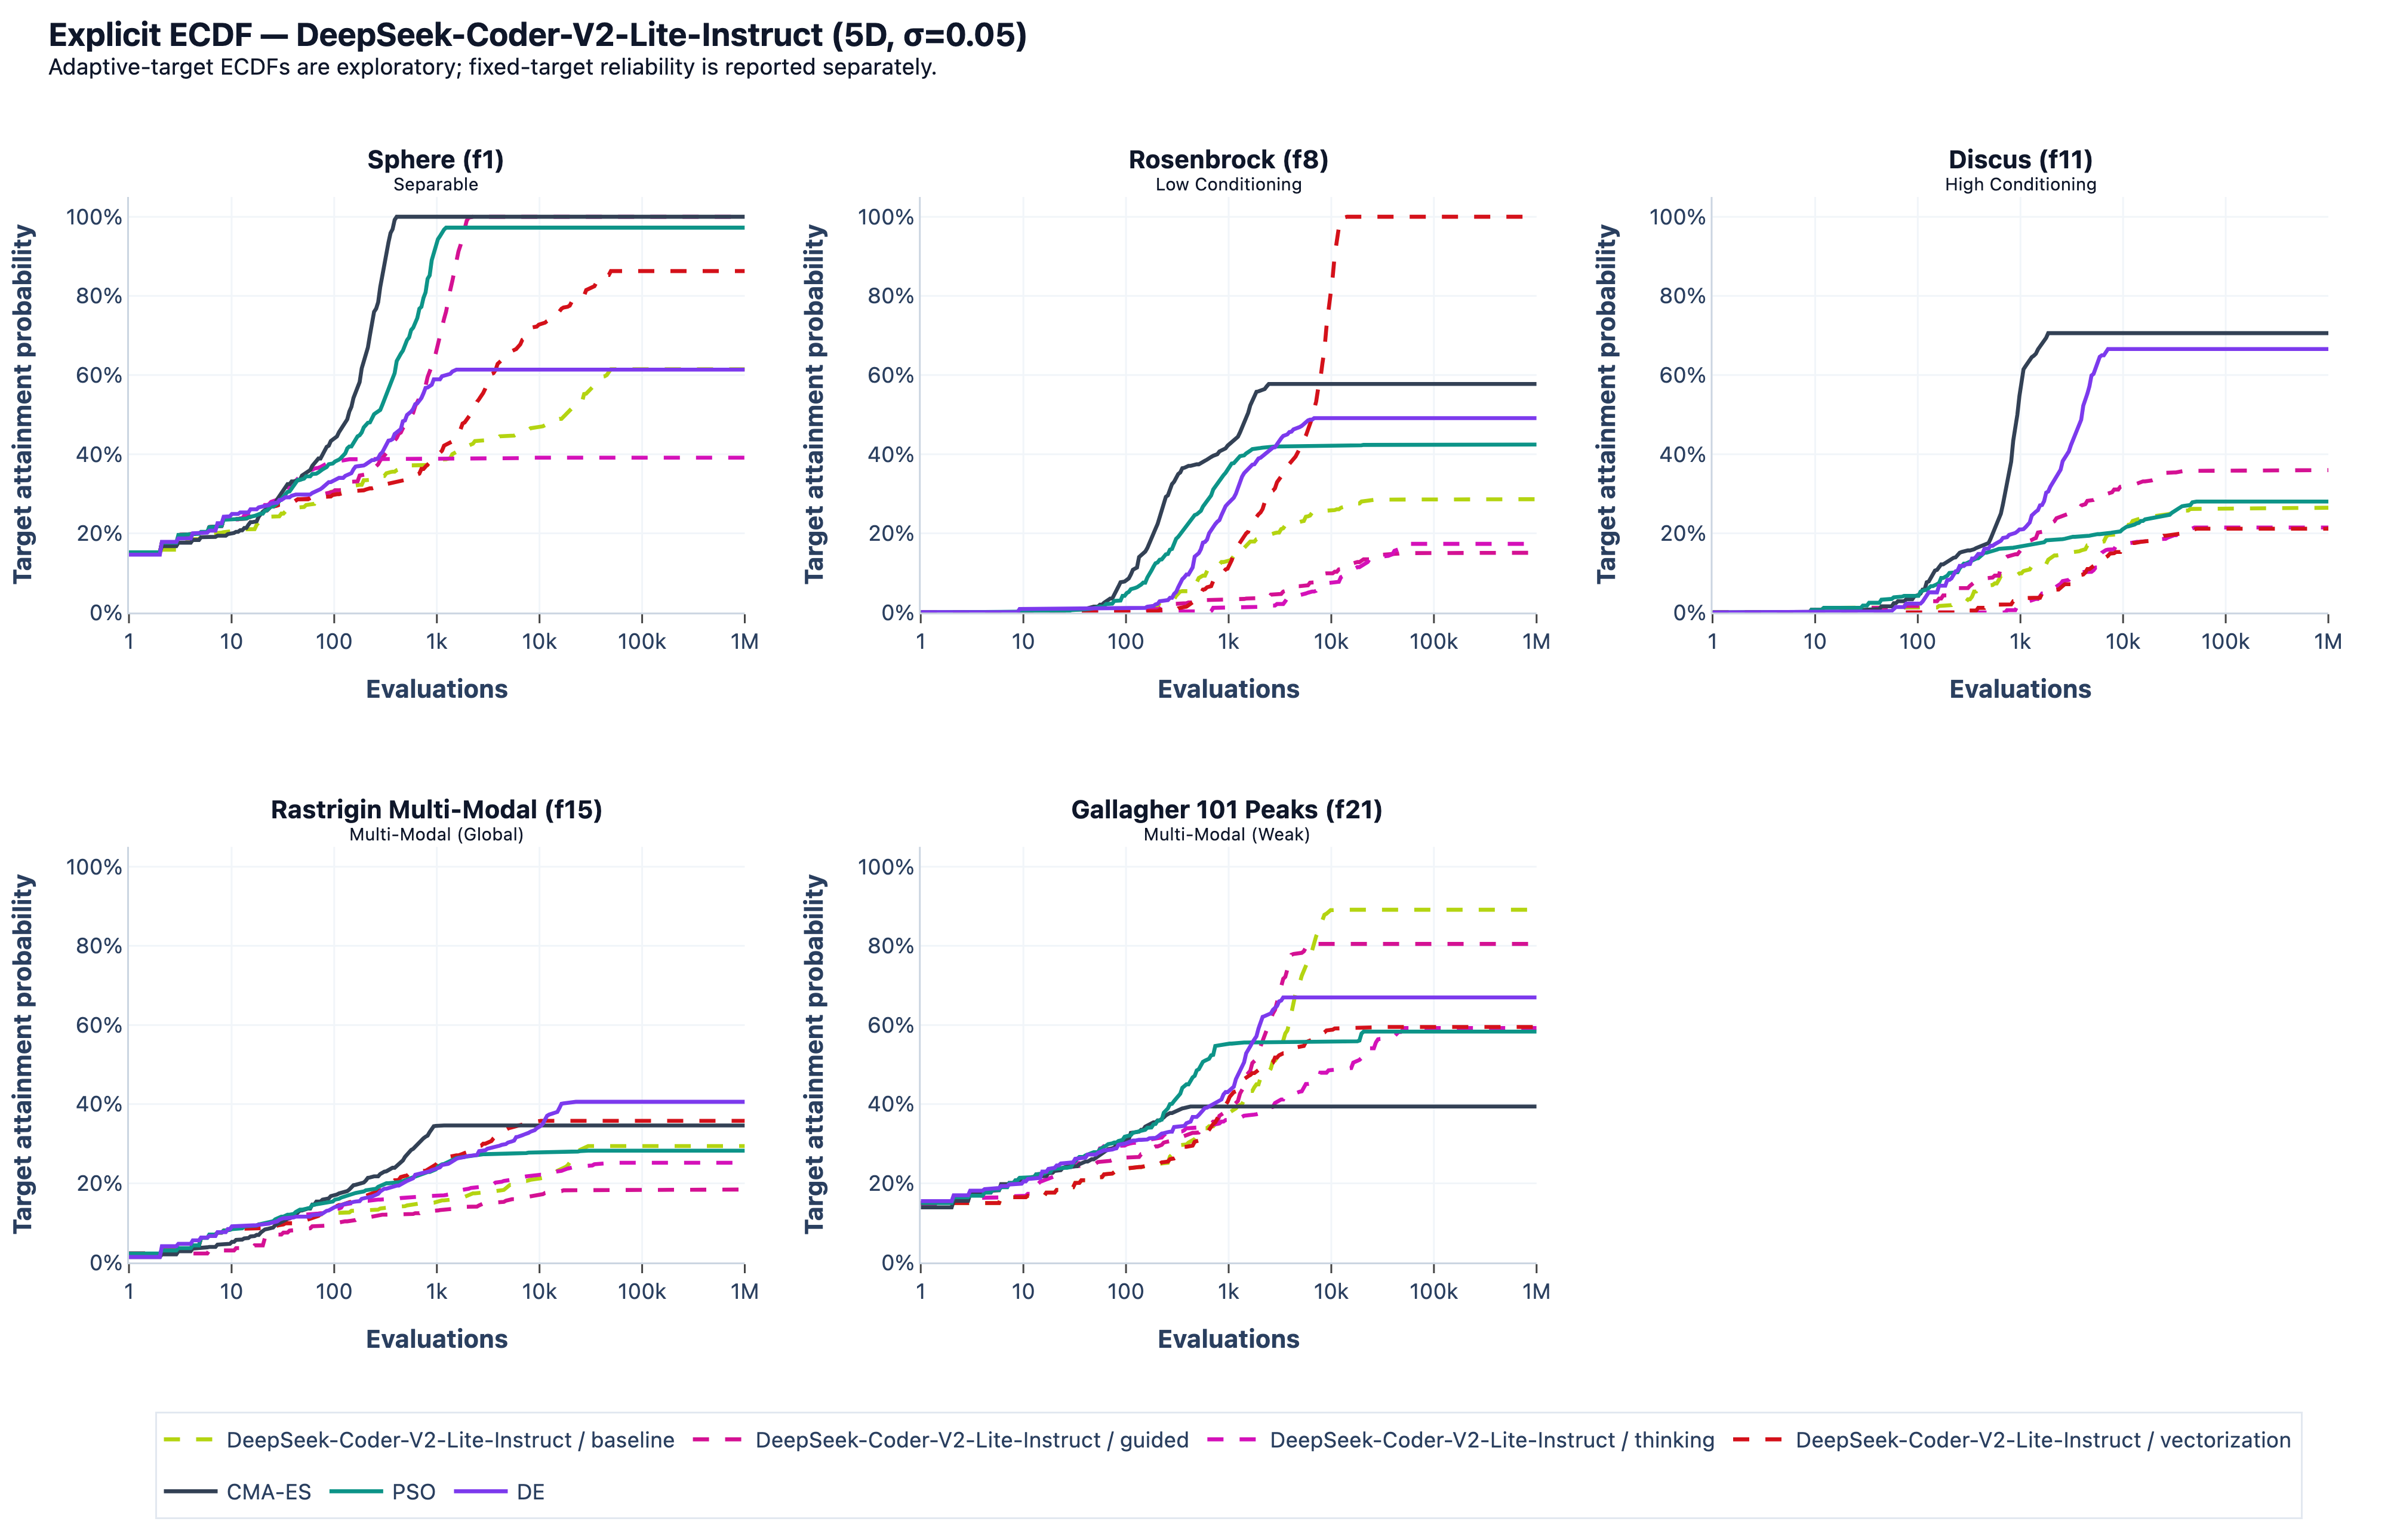
\includegraphics[width=\textwidth,height=0.32\textheight,keepaspectratio]{images/experiments/02_explicit/deepseek_coder_v2_lite_instruct_q4_k_m/5D/std_0.05/target_precision_ecdf.png}
    \caption{DeepSeek-Coder-V2-Lite-Instruct: Explicit, $D=5$,
    $\sigma=0.05$. Convergence (median and IQR) above;
    adaptive target-precision ECDF below. The objective-query allowance
    is 50,000.}
    \label{fig:appendix_02_explicit_deepseek_coder_v2_lite_instruct_q4_k_m_5_std_005}
\end{minipage}
\par\medskip

\section{Implicit Profiles}
\nopagebreak[4]

\subsection{Qwen2.5-Coder-14B-Instruct}
\nopagebreak[4]

\par\smallskip\noindent
\begin{minipage}{\linewidth}
    \captionsetup{type=figure,aboveskip=4pt,belowskip=0pt}
    \centering
    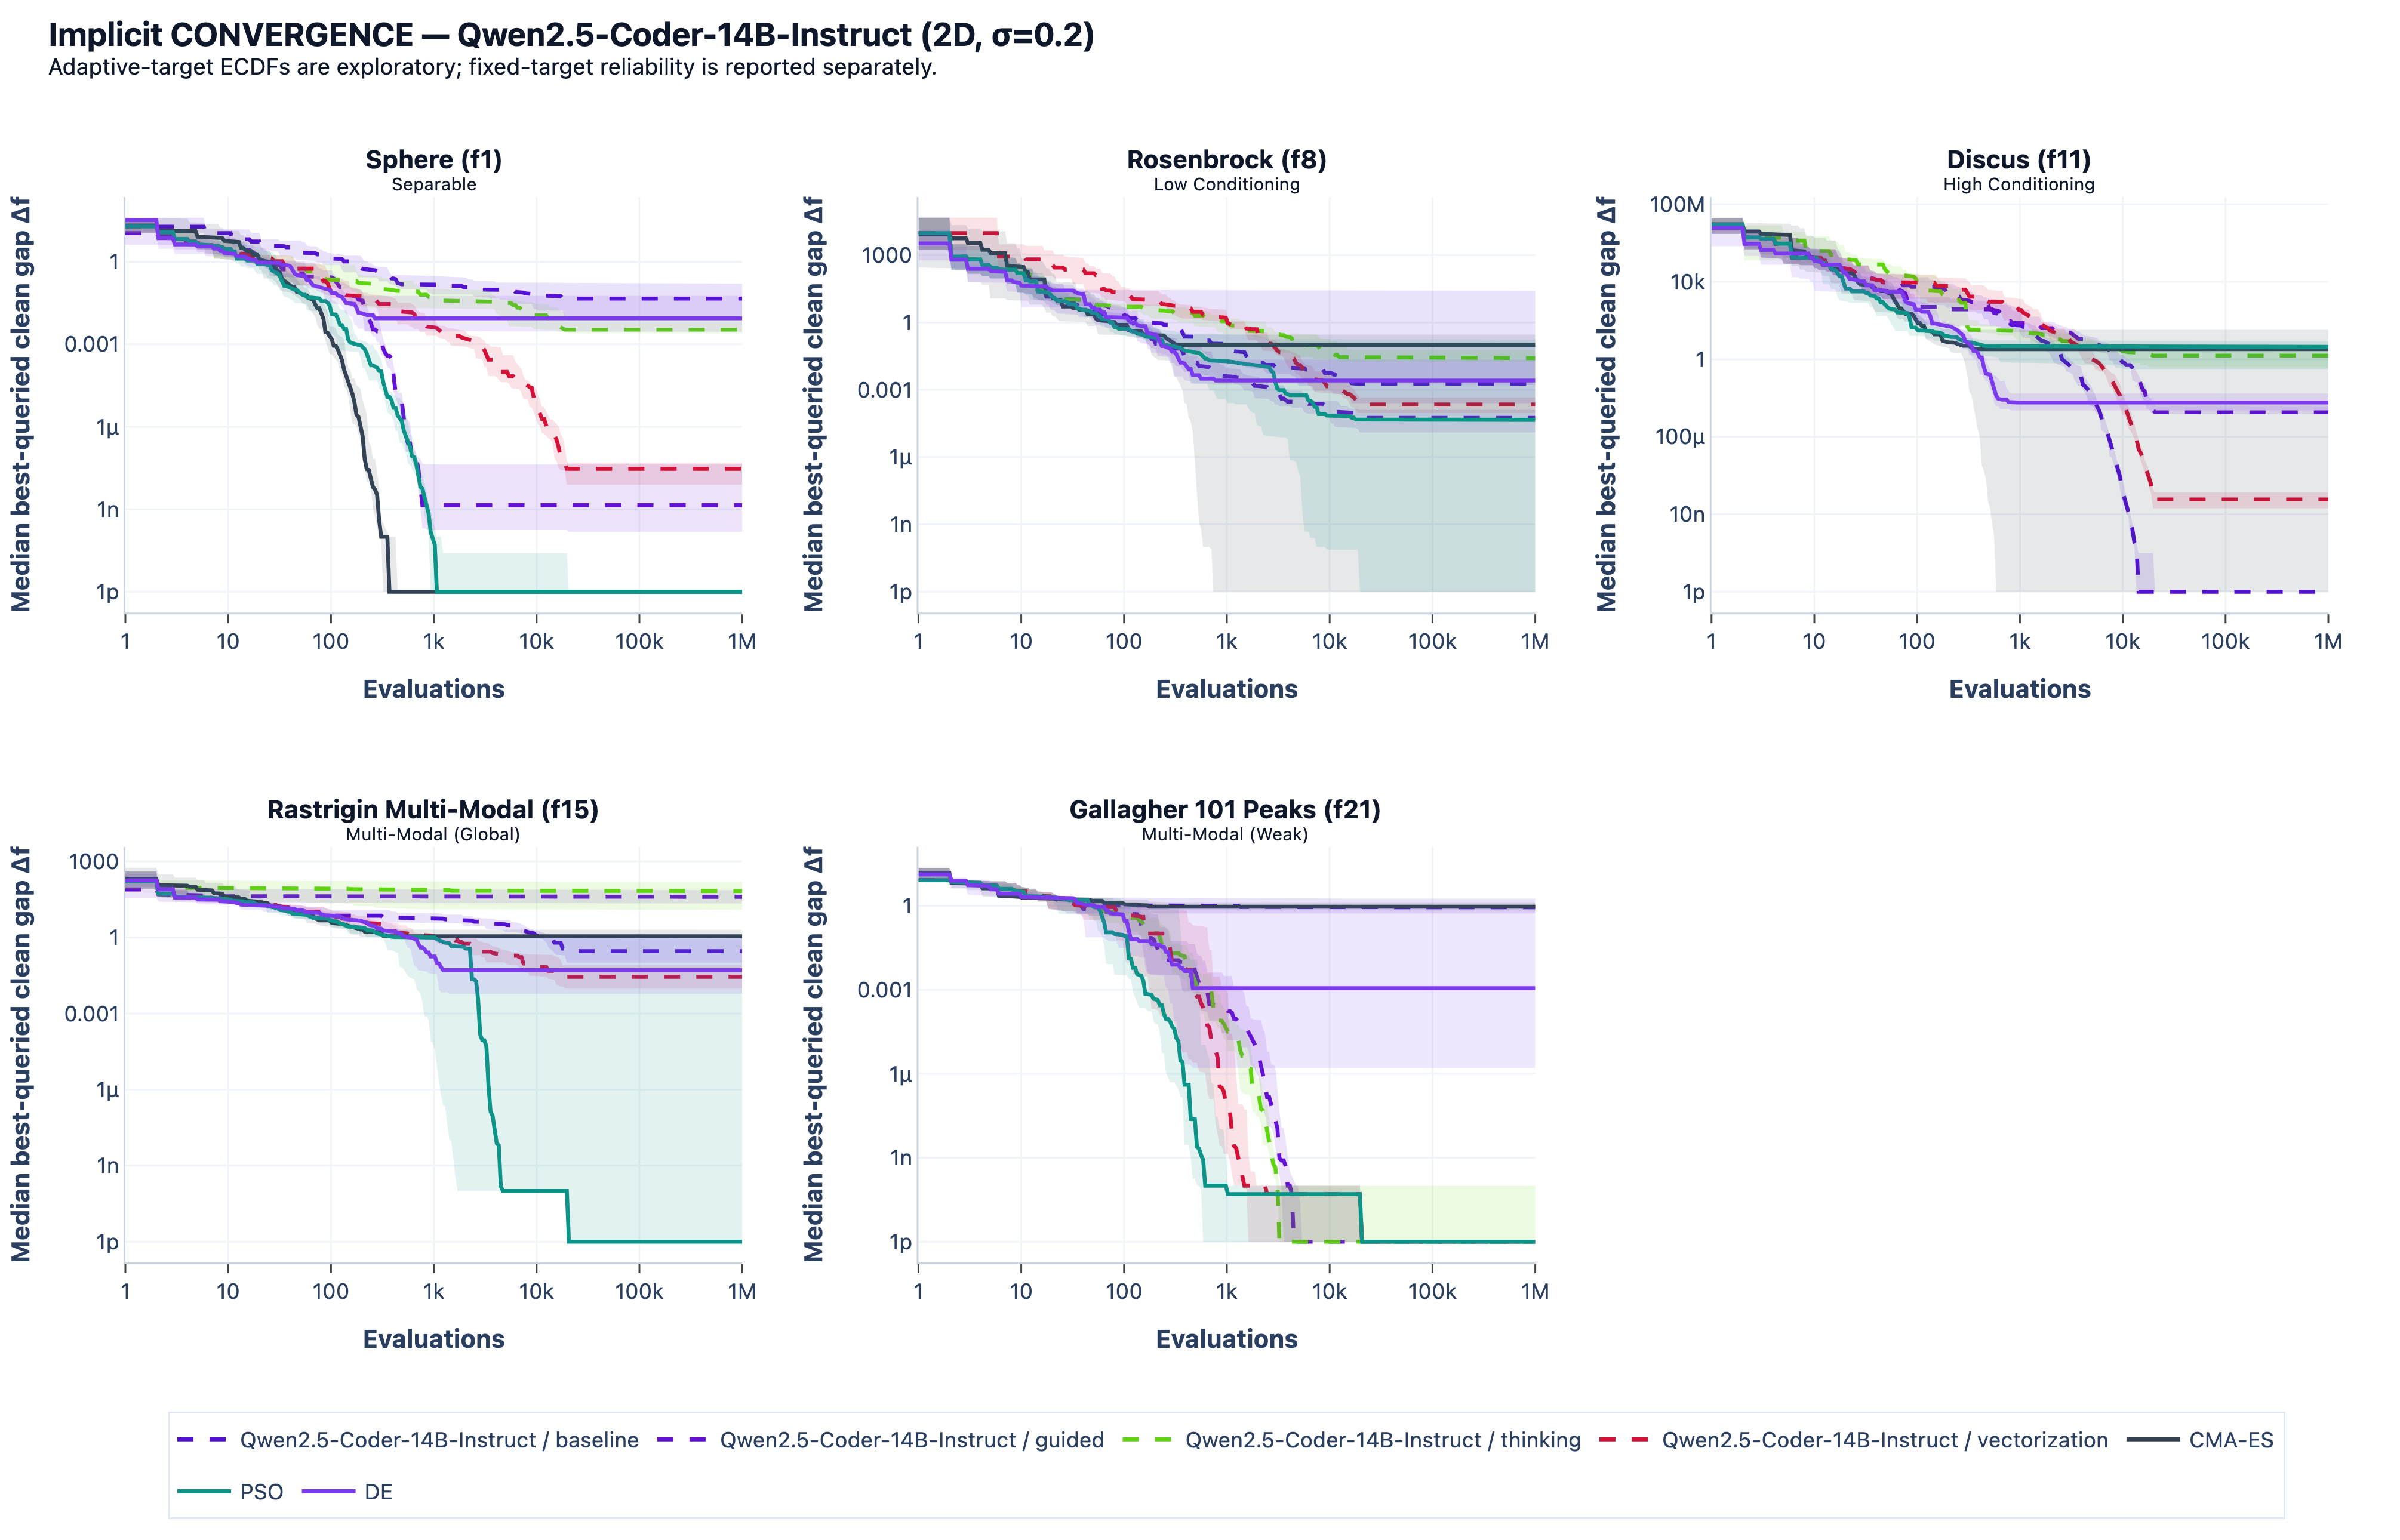
\includegraphics[width=\textwidth,height=0.32\textheight,keepaspectratio]{images/experiments/03_implicit/qwen_14b/2D/std_0.2/convergence_trajectories.png}
    \par\medskip
    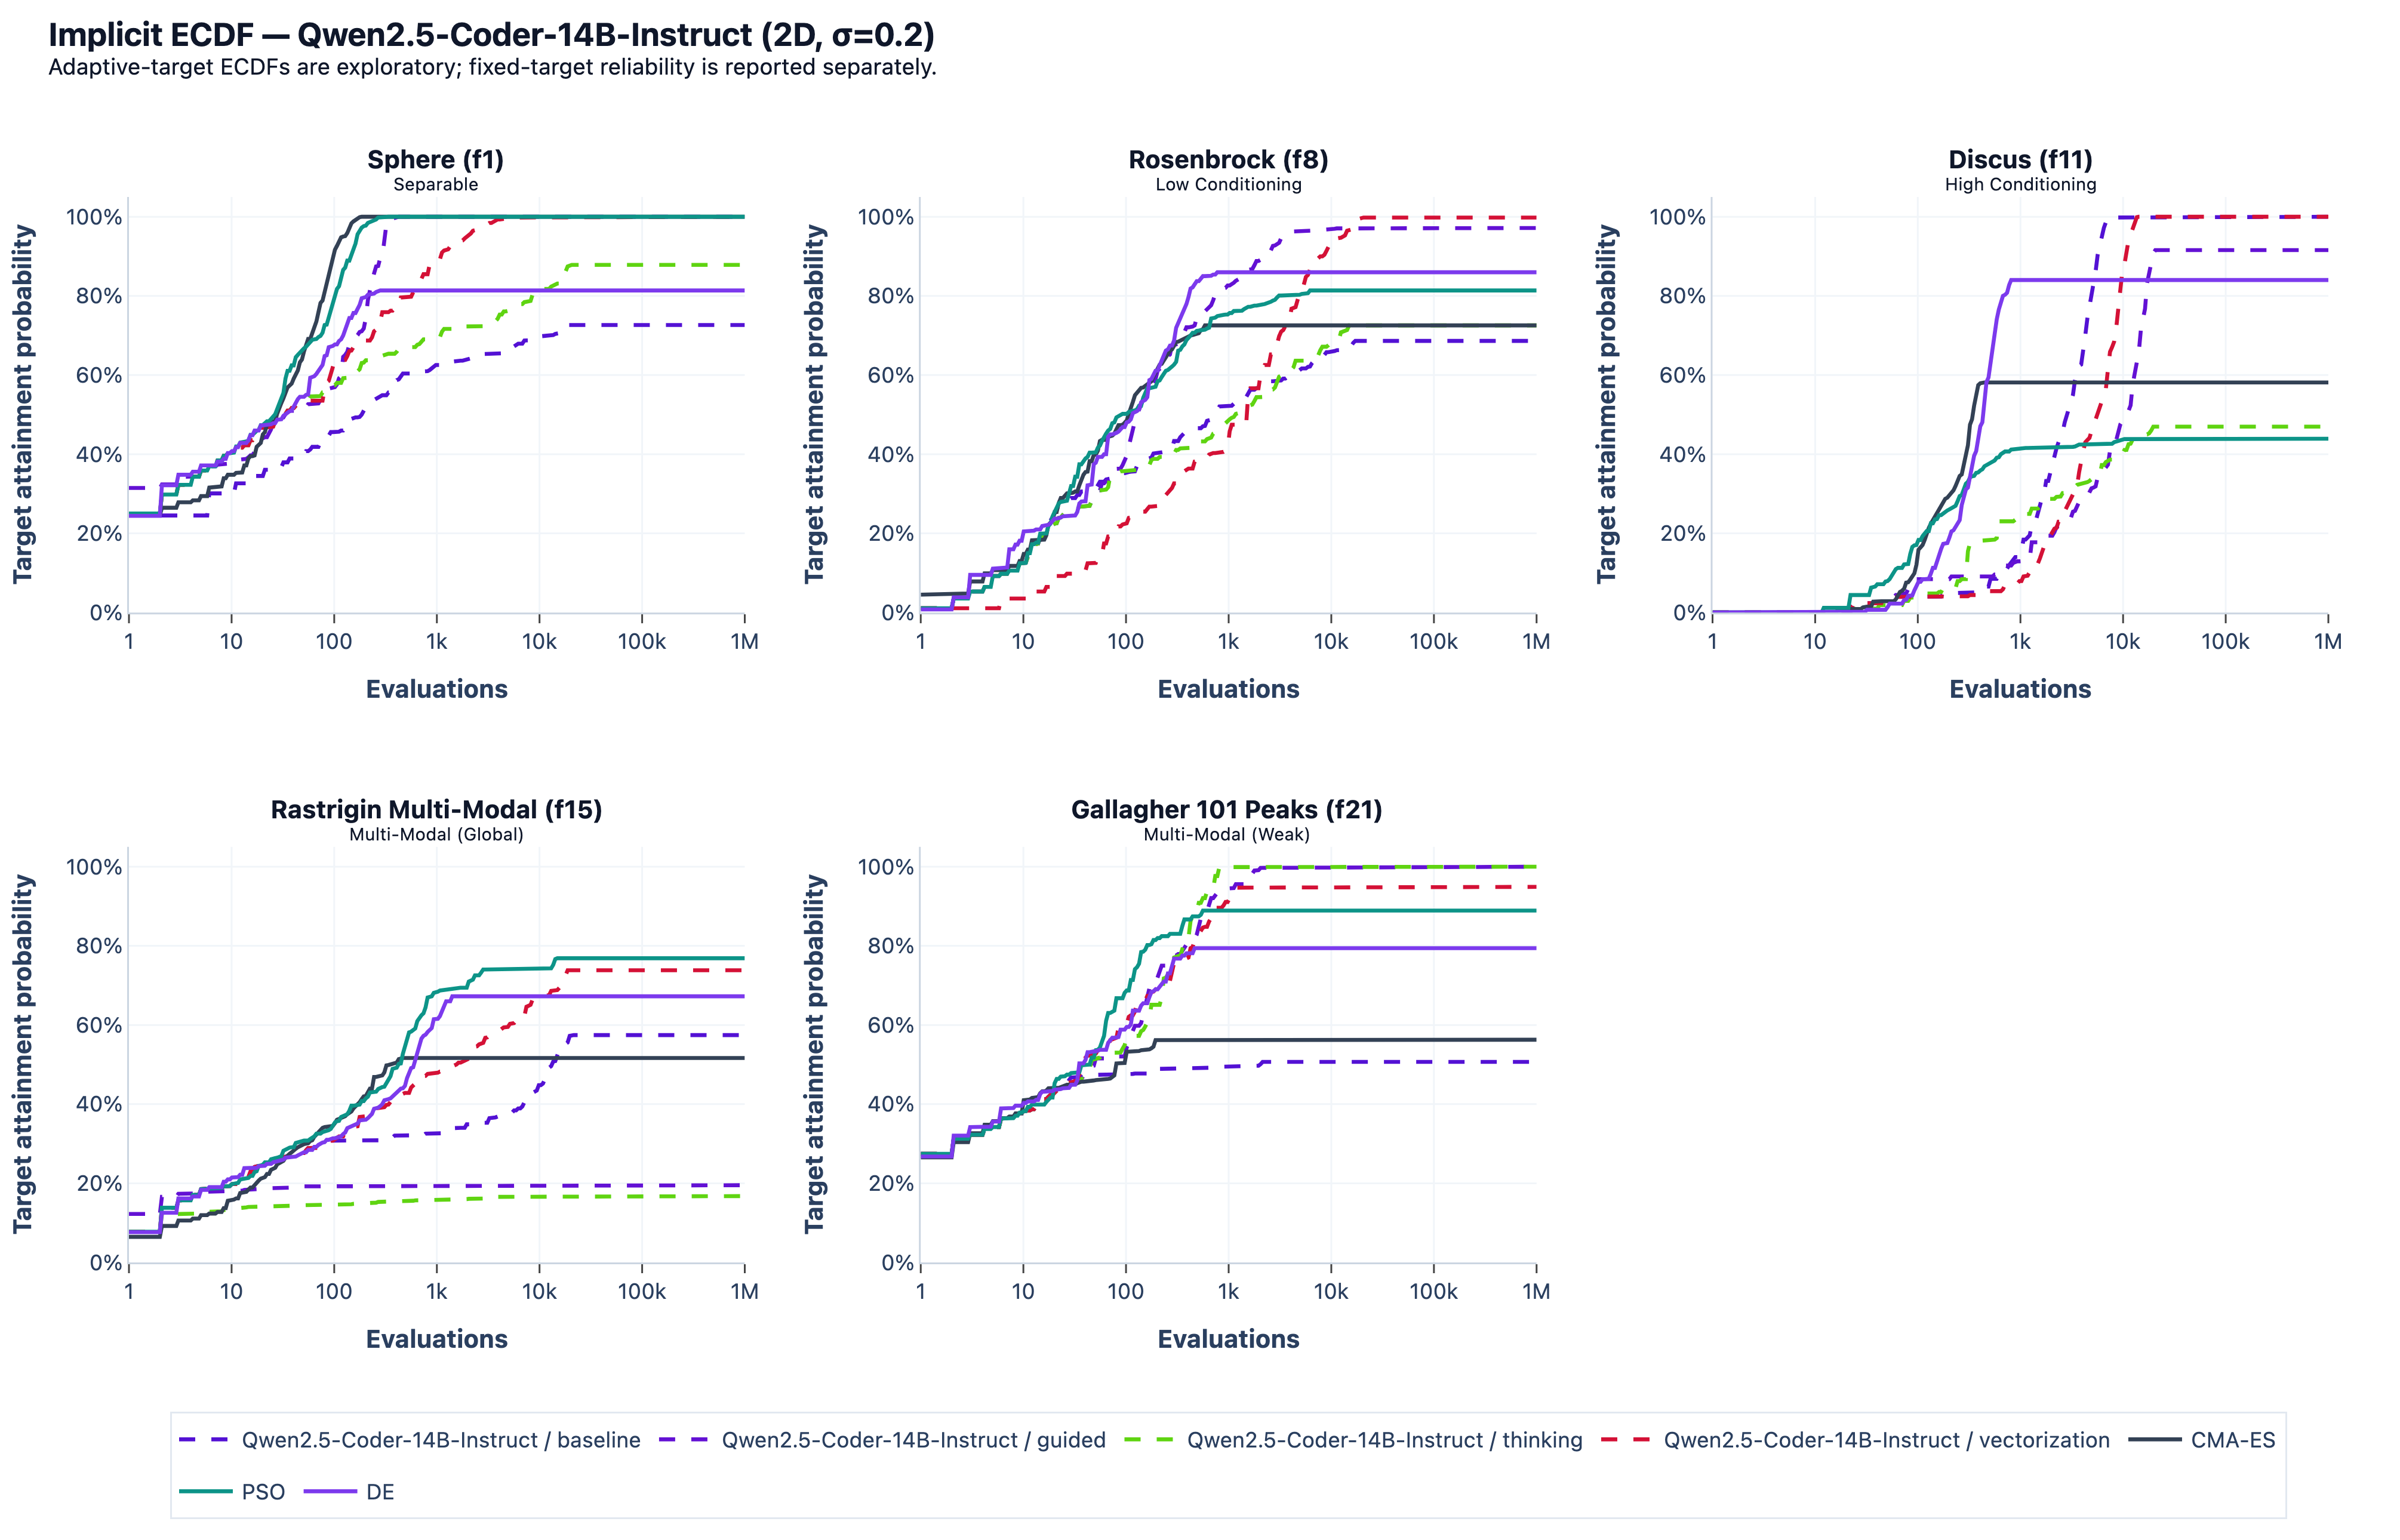
\includegraphics[width=\textwidth,height=0.32\textheight,keepaspectratio]{images/experiments/03_implicit/qwen_14b/2D/std_0.2/target_precision_ecdf.png}
    \caption{Qwen2.5-Coder-14B-Instruct: Implicit, $D=2$,
    $\sigma=0.2$. Convergence (median and IQR) above;
    adaptive target-precision ECDF below. The objective-query allowance
    is 20,000.}
    \label{fig:appendix_03_implicit_qwen_14b_2_std_02}
\end{minipage}
\par\medskip

\par\smallskip\noindent
\begin{minipage}{\linewidth}
    \captionsetup{type=figure,aboveskip=4pt,belowskip=0pt}
    \centering
    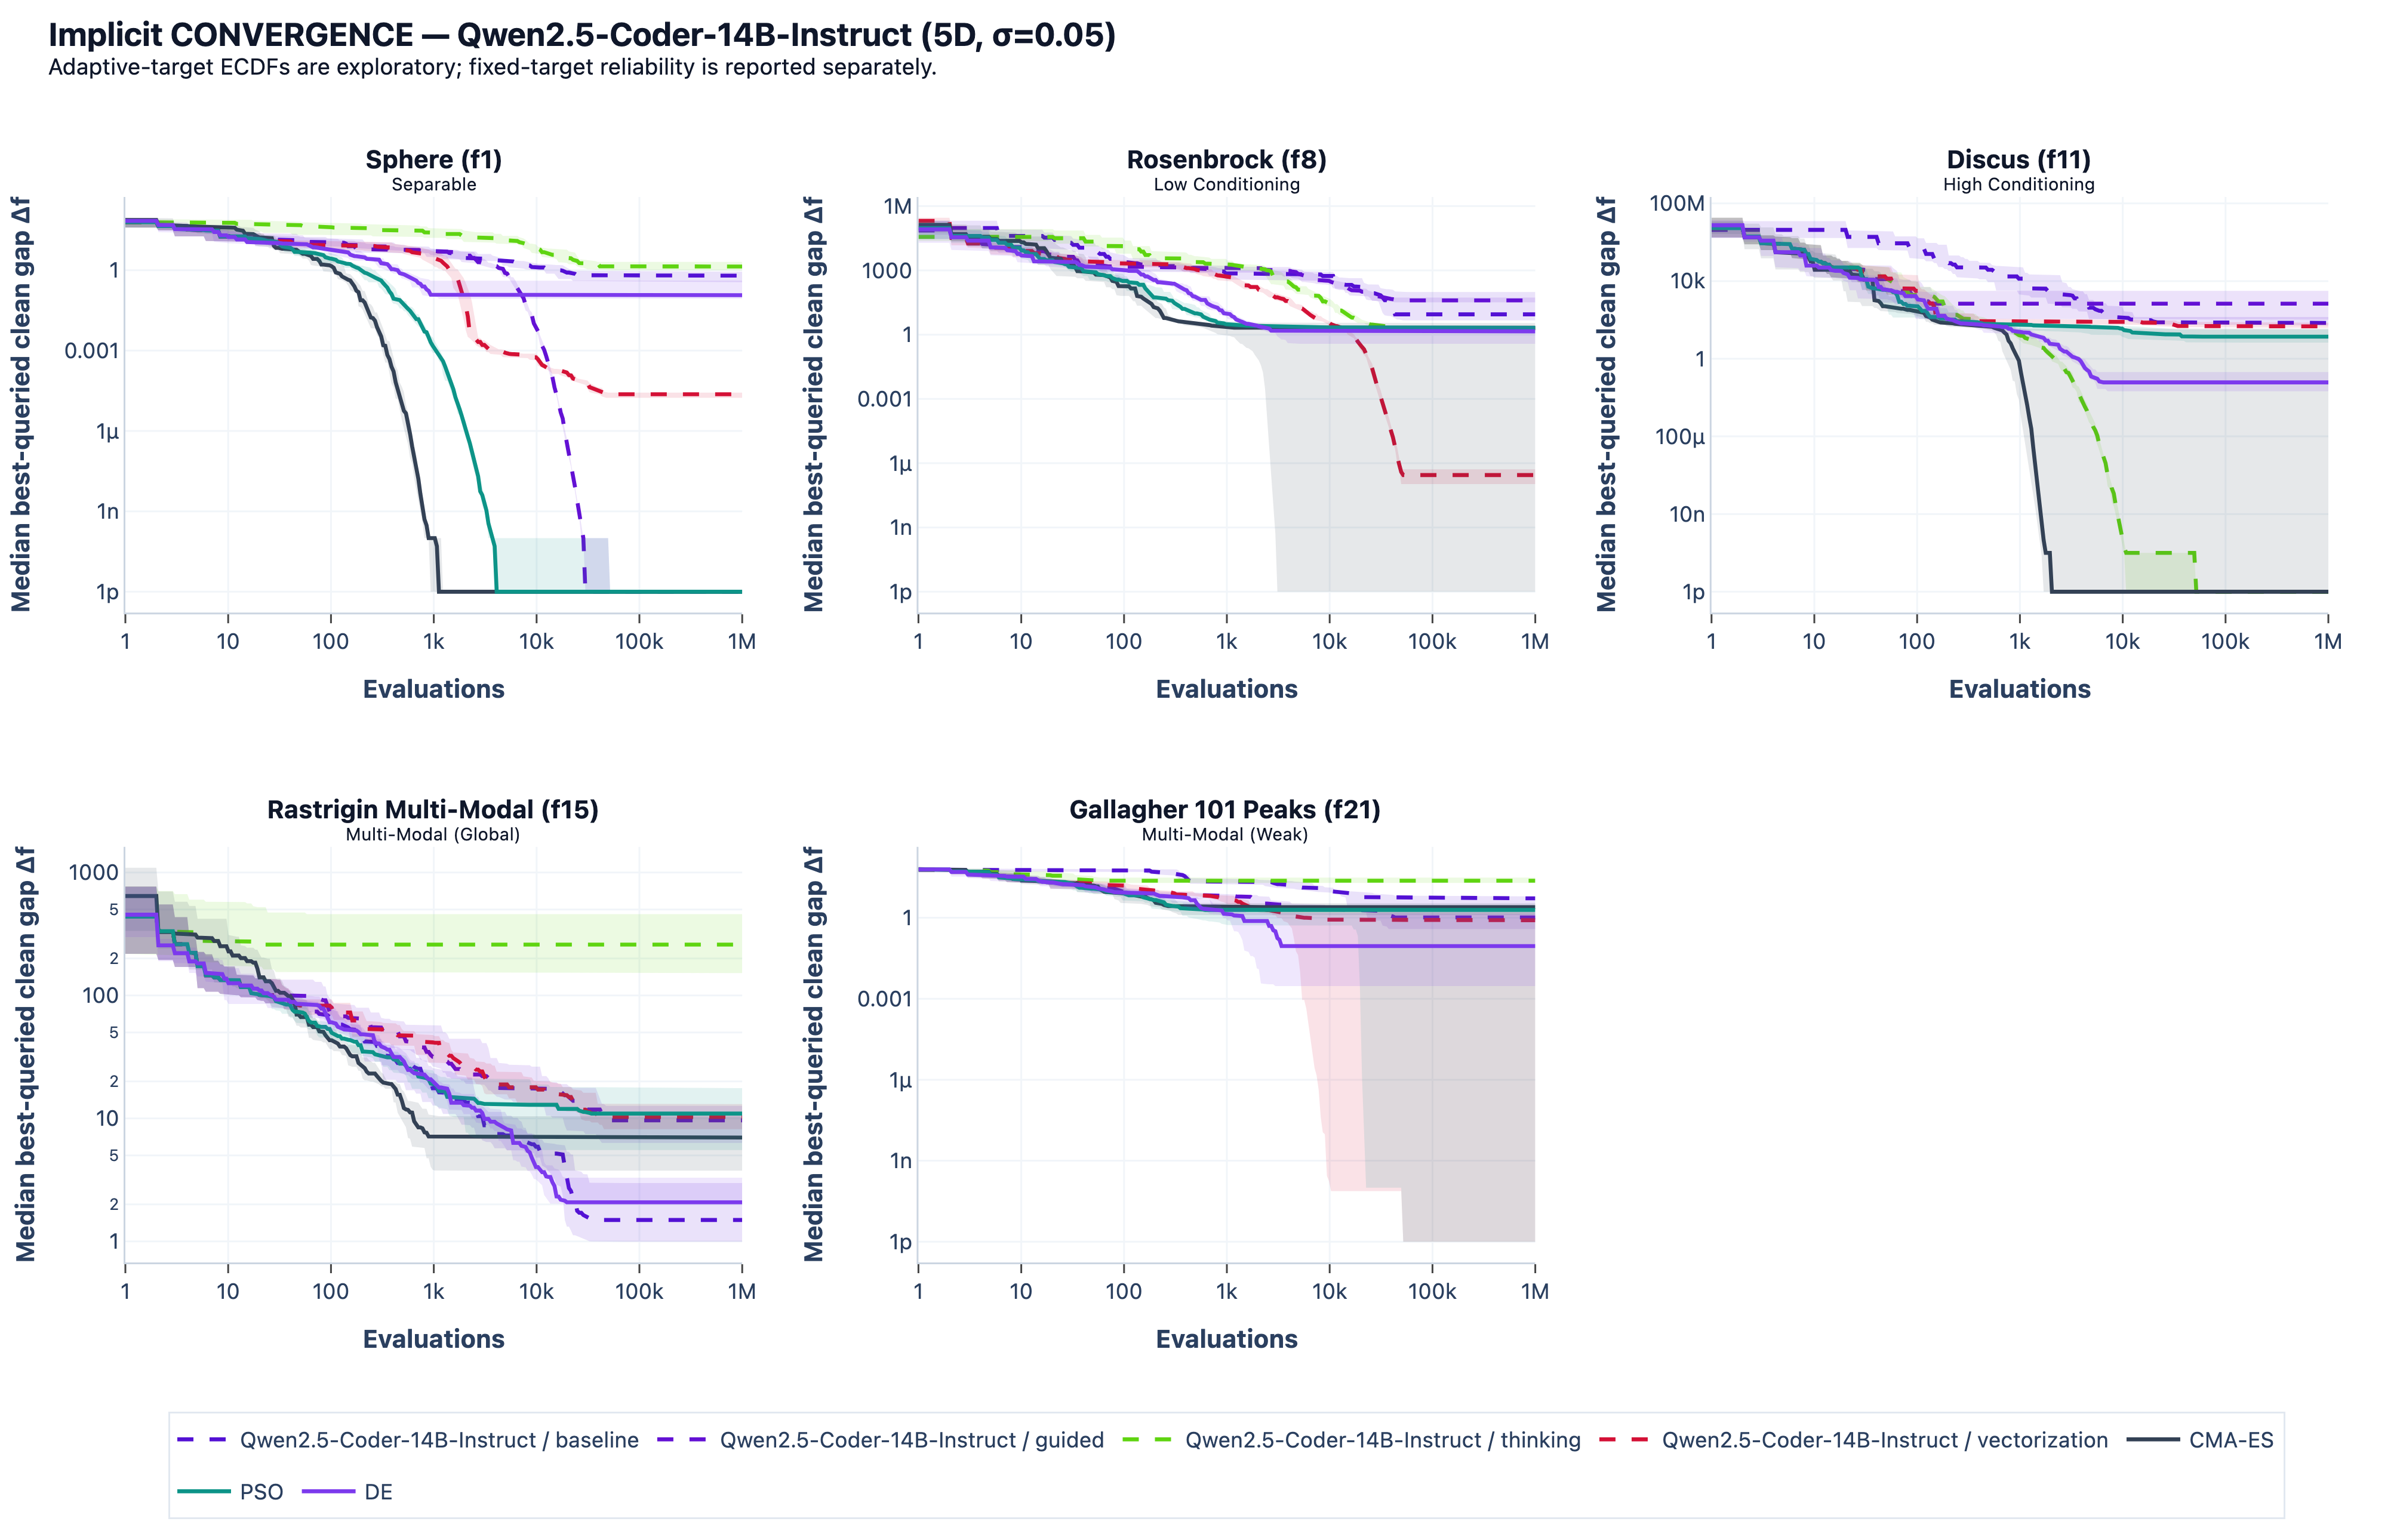
\includegraphics[width=\textwidth,height=0.32\textheight,keepaspectratio]{images/experiments/03_implicit/qwen_14b/5D/std_0.05/convergence_trajectories.png}
    \par\medskip
    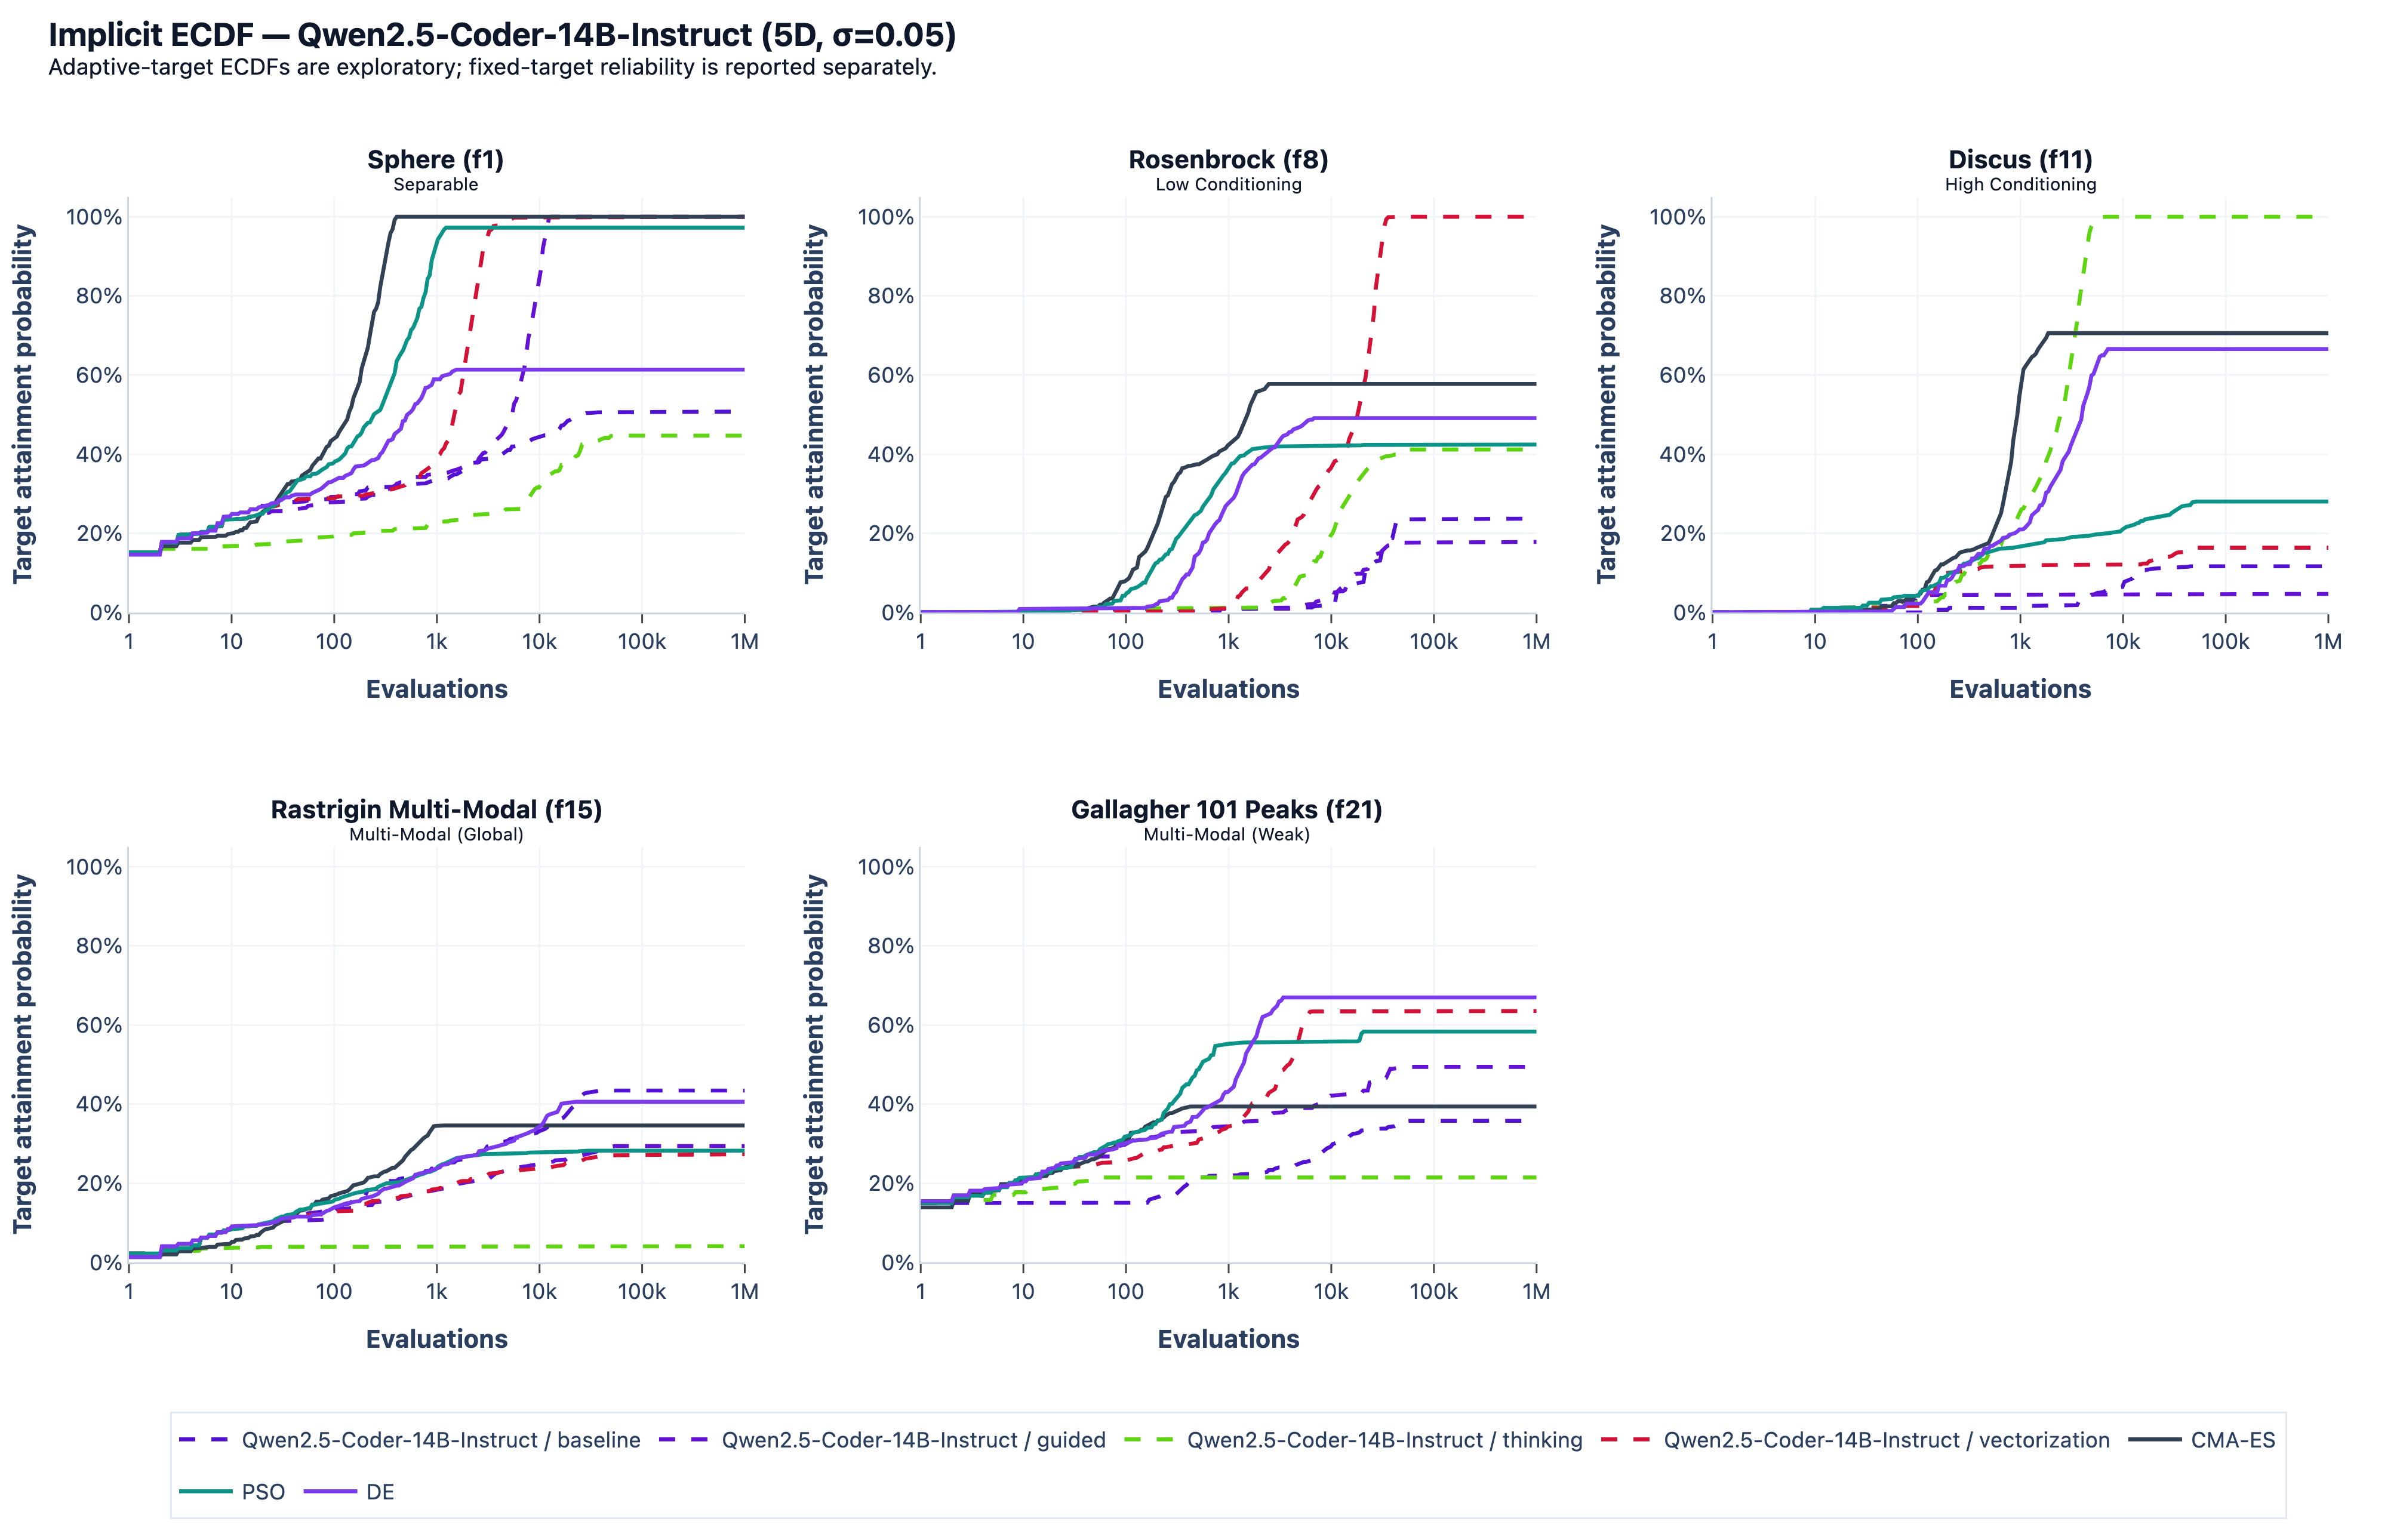
\includegraphics[width=\textwidth,height=0.32\textheight,keepaspectratio]{images/experiments/03_implicit/qwen_14b/5D/std_0.05/target_precision_ecdf.png}
    \caption{Qwen2.5-Coder-14B-Instruct: Implicit, $D=5$,
    $\sigma=0.05$. Convergence (median and IQR) above;
    adaptive target-precision ECDF below. The objective-query allowance
    is 50,000.}
    \label{fig:appendix_03_implicit_qwen_14b_5_std_005}
\end{minipage}
\par\medskip

\par\smallskip\noindent
\begin{minipage}{\linewidth}
    \captionsetup{type=figure,aboveskip=4pt,belowskip=0pt}
    \centering
    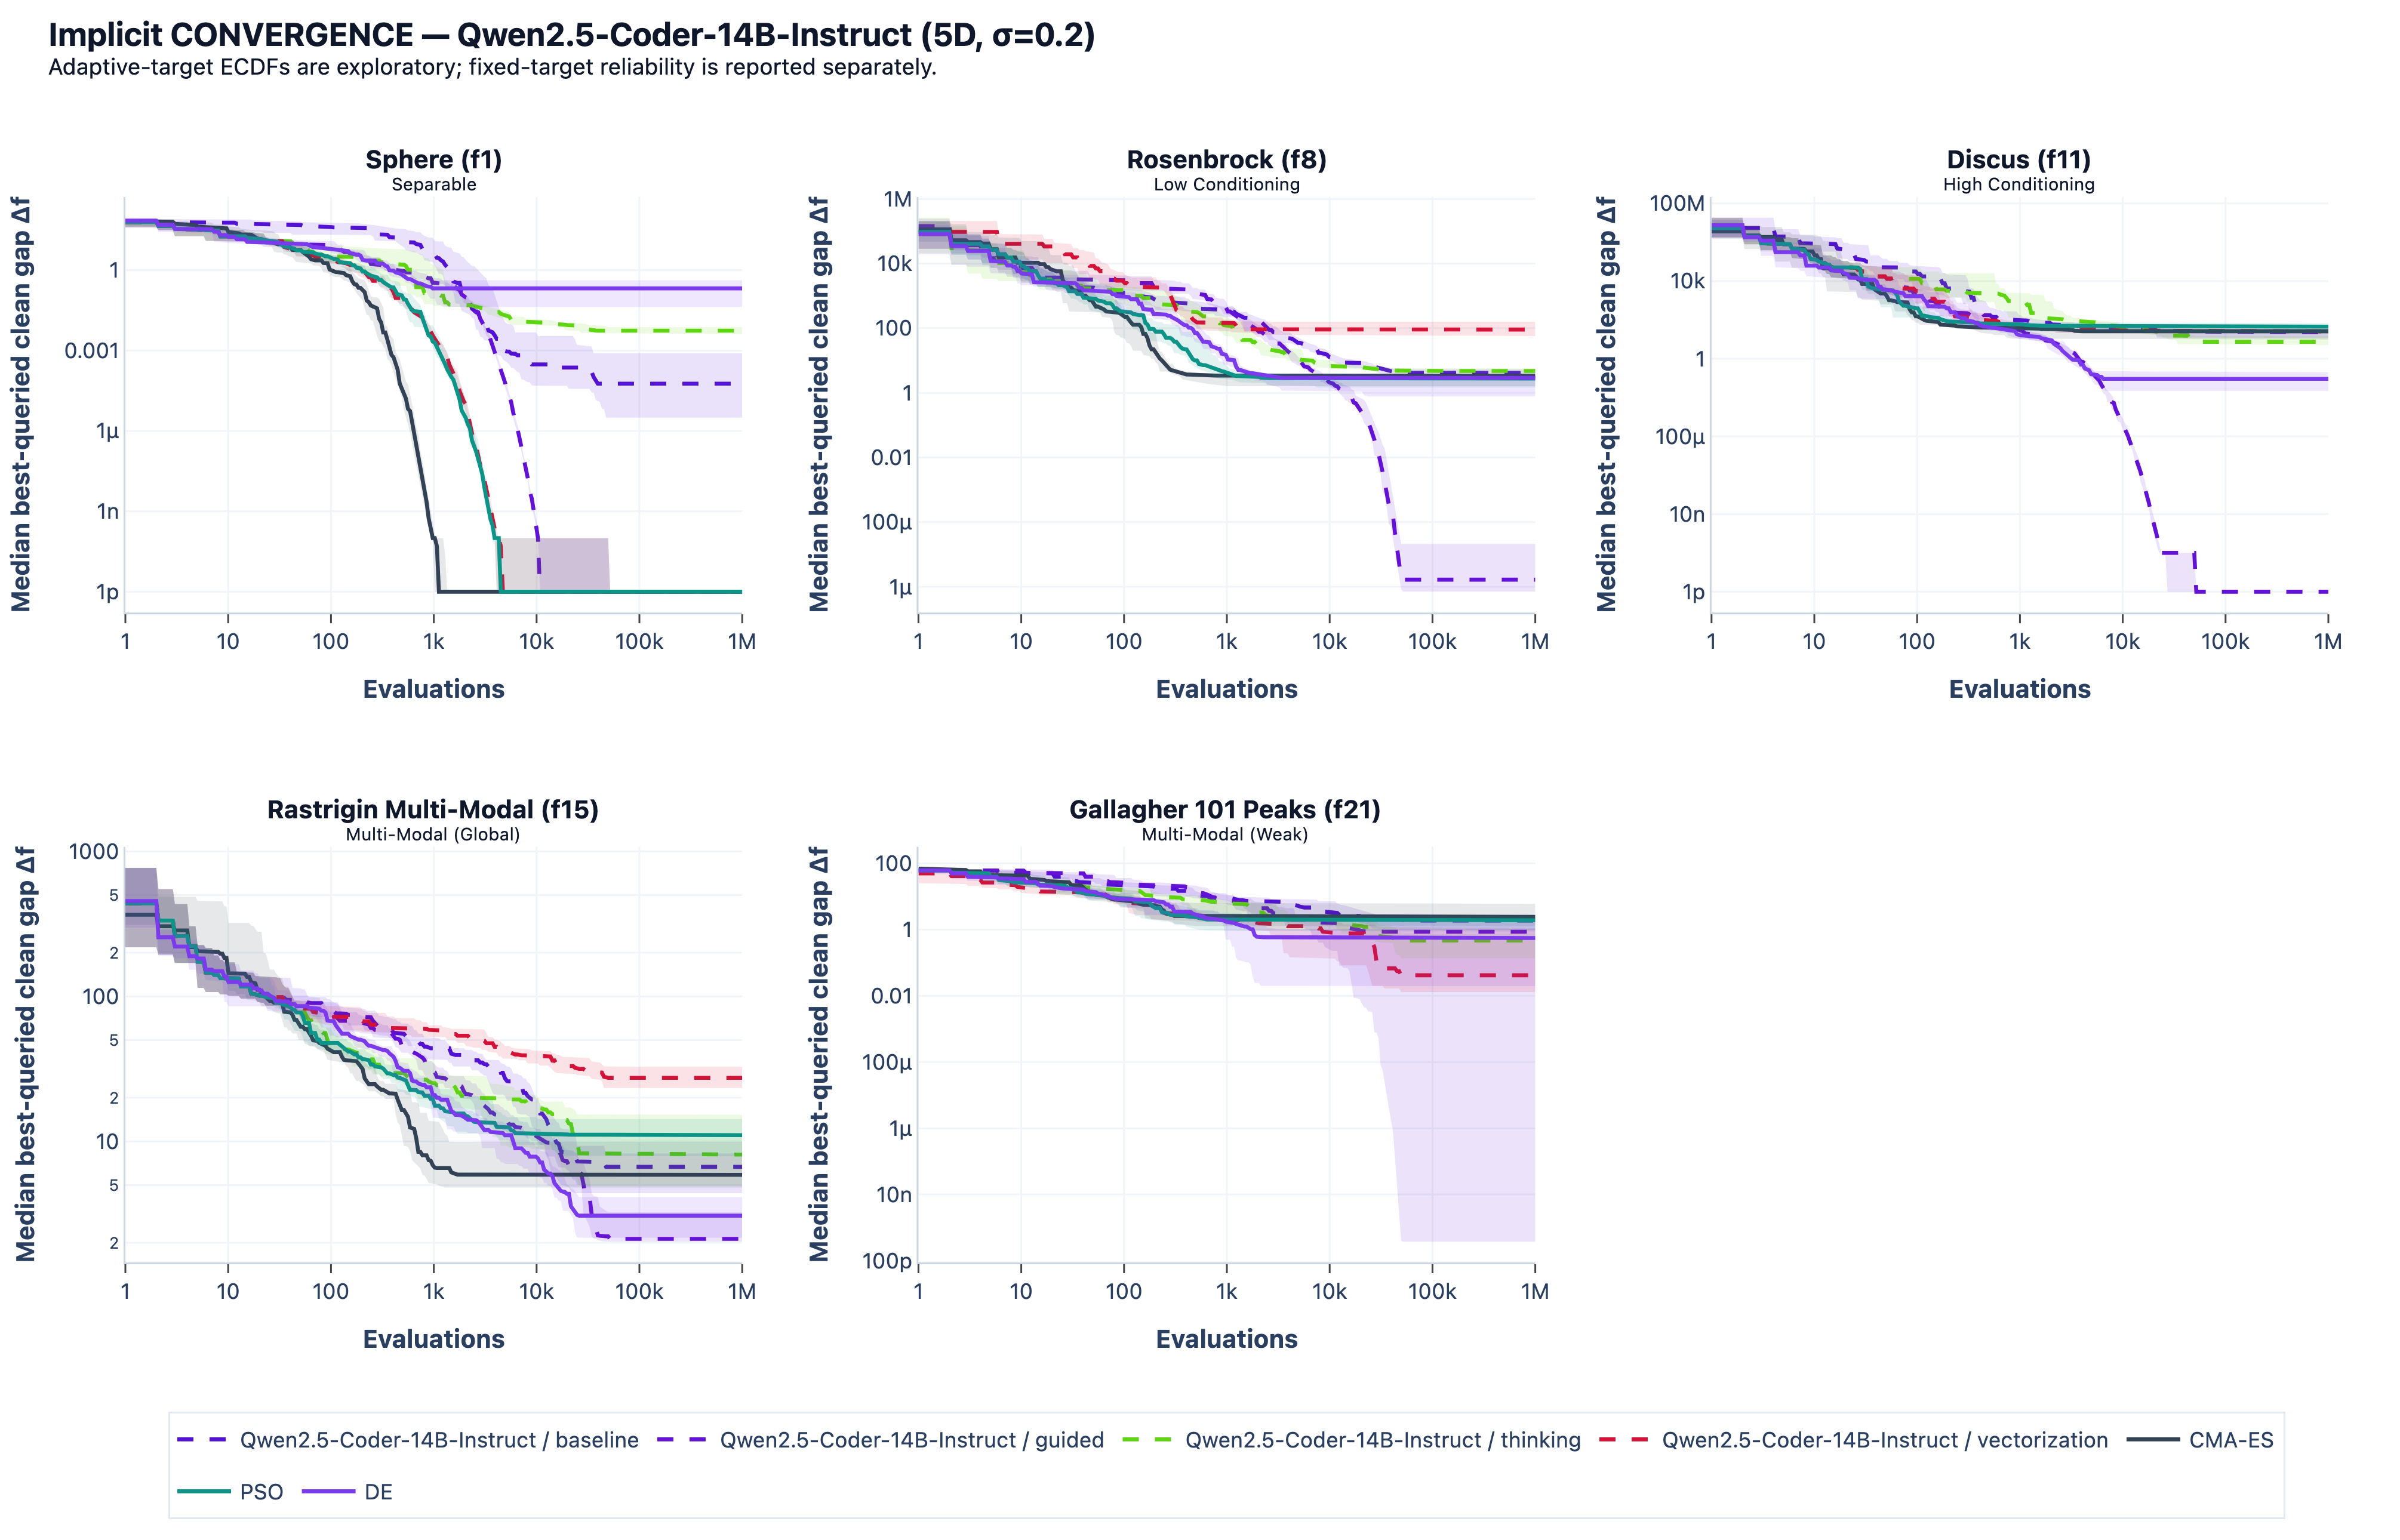
\includegraphics[width=\textwidth,height=0.32\textheight,keepaspectratio]{images/experiments/03_implicit/qwen_14b/5D/std_0.2/convergence_trajectories.png}
    \par\medskip
    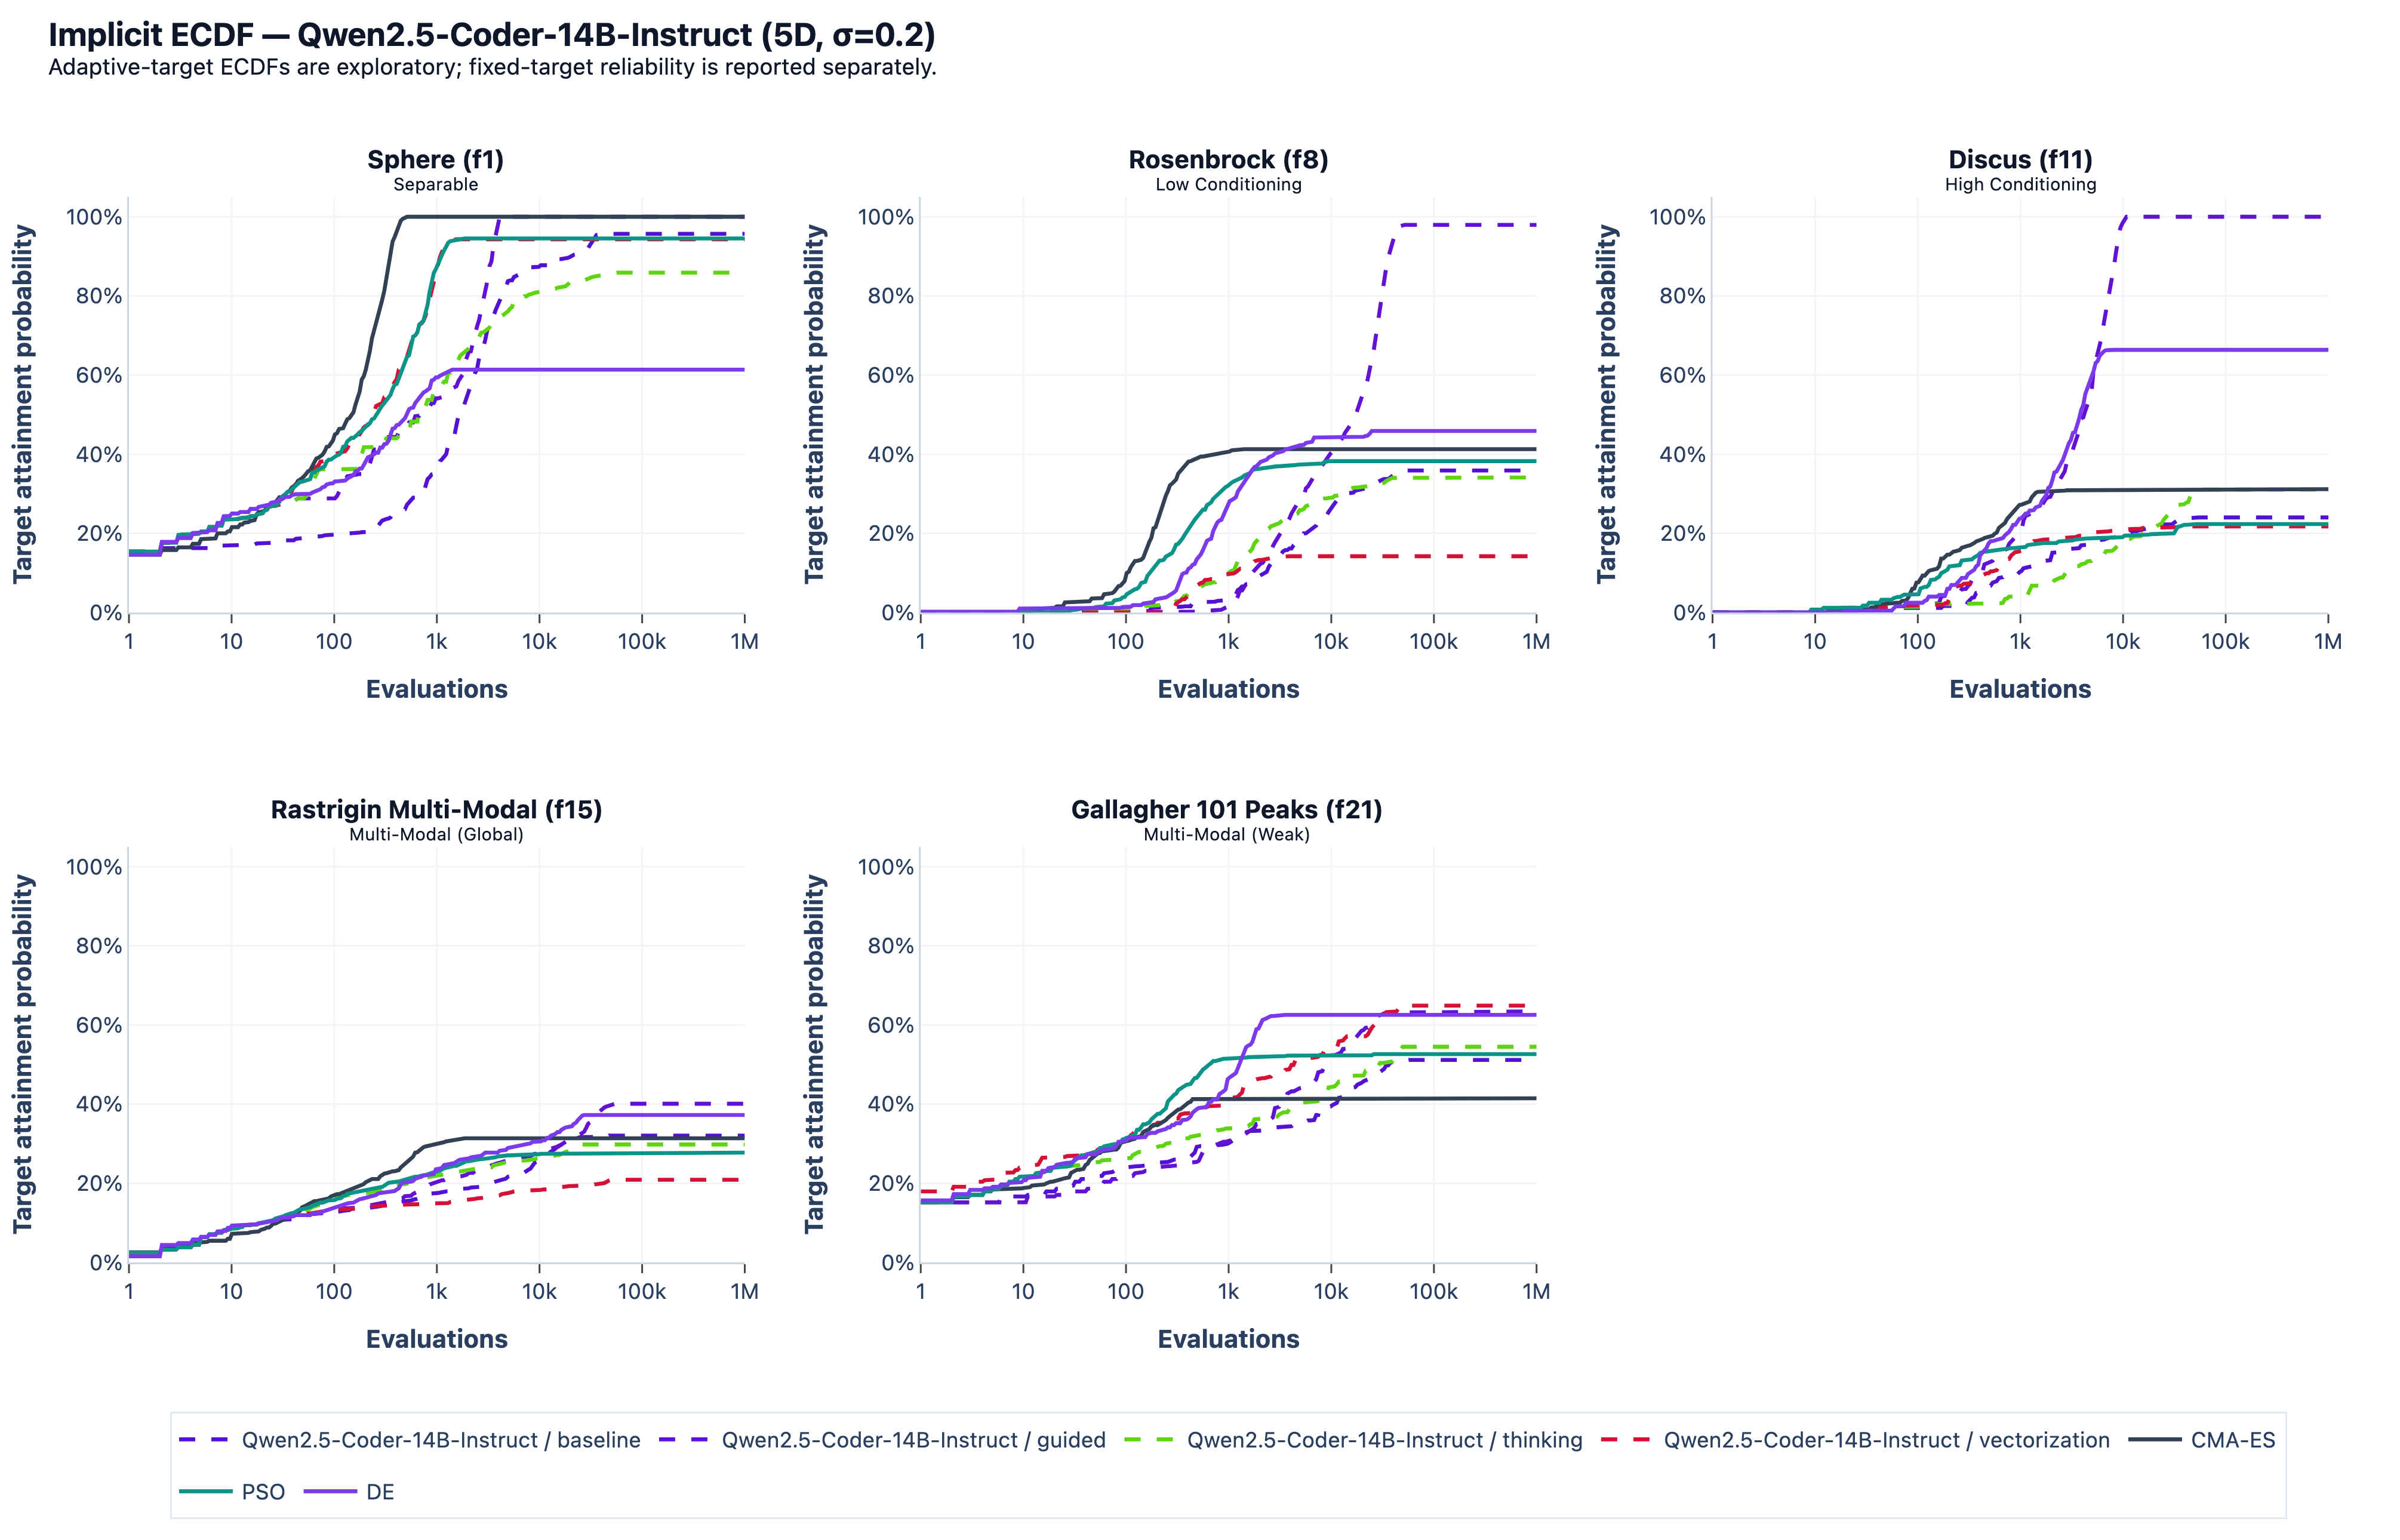
\includegraphics[width=\textwidth,height=0.32\textheight,keepaspectratio]{images/experiments/03_implicit/qwen_14b/5D/std_0.2/target_precision_ecdf.png}
    \caption{Qwen2.5-Coder-14B-Instruct: Implicit, $D=5$,
    $\sigma=0.2$. Convergence (median and IQR) above;
    adaptive target-precision ECDF below. The objective-query allowance
    is 50,000.}
    \label{fig:appendix_03_implicit_qwen_14b_5_std_02}
\end{minipage}
\par\medskip

\subsection{Qwen2.5-Coder-32B-Instruct}
\nopagebreak[4]

\par\smallskip\noindent
\begin{minipage}{\linewidth}
    \captionsetup{type=figure,aboveskip=4pt,belowskip=0pt}
    \centering
    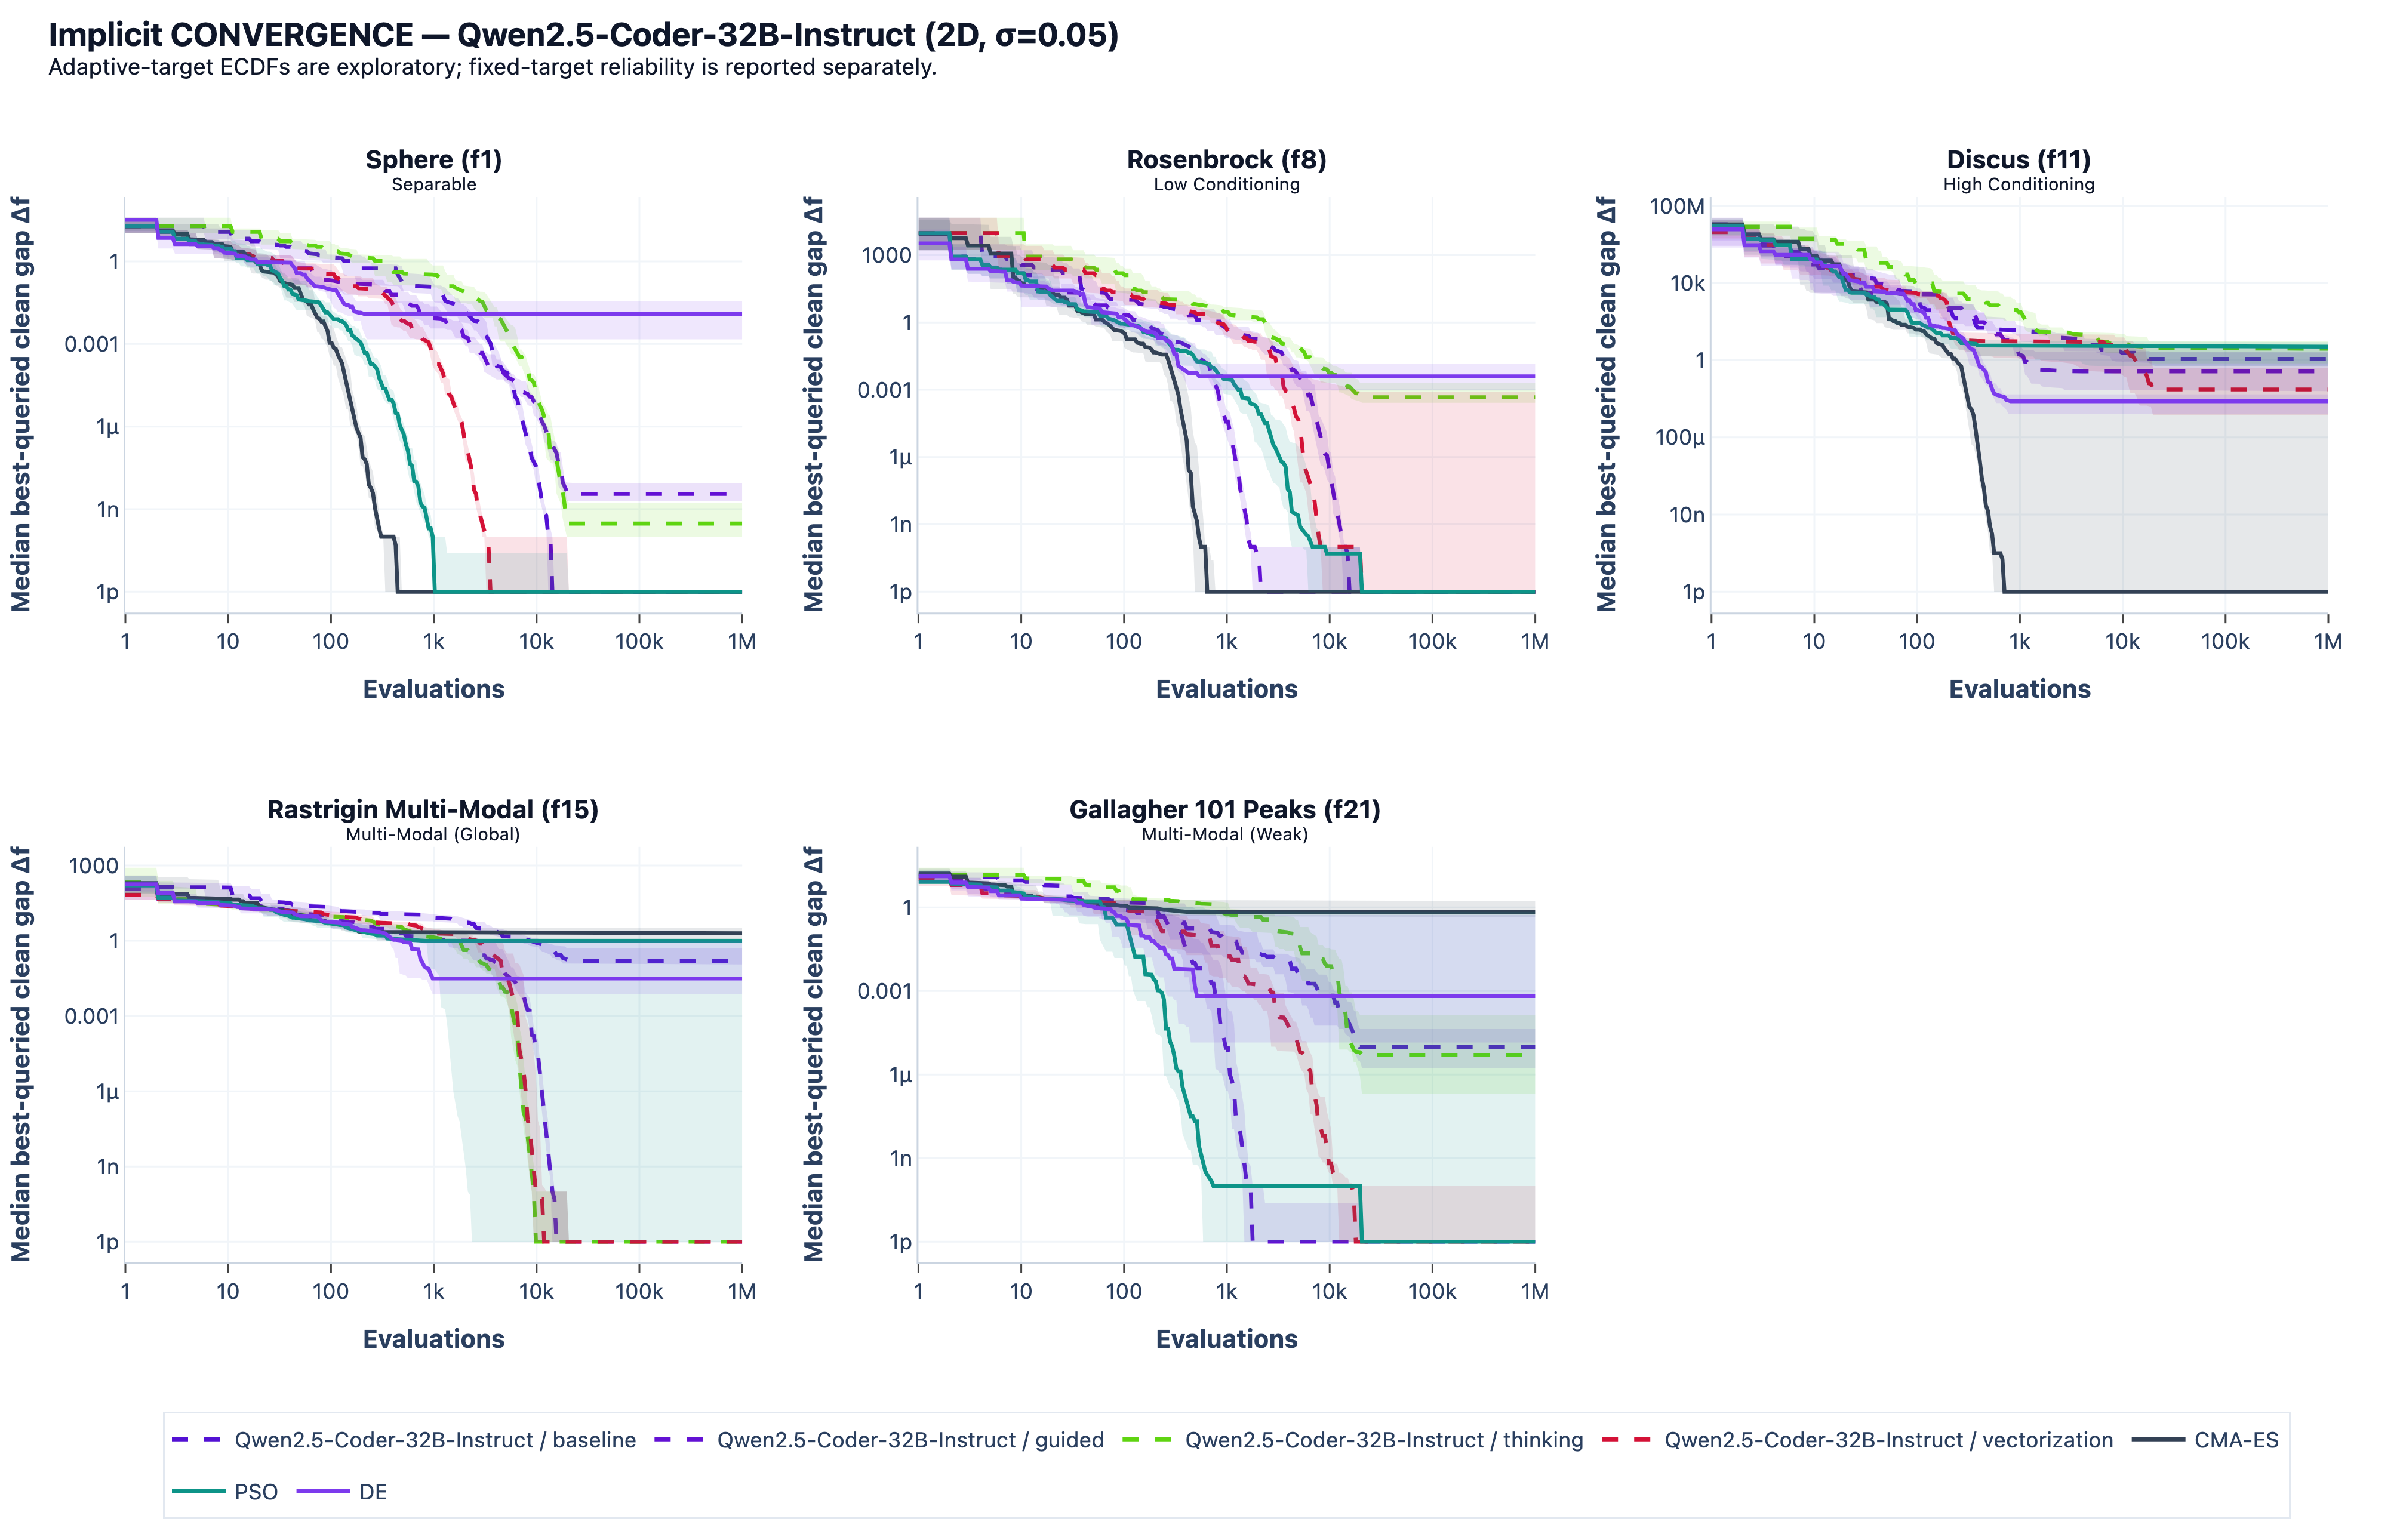
\includegraphics[width=\textwidth,height=0.32\textheight,keepaspectratio]{images/experiments/03_implicit/qwen_32b/2D/std_0.05/convergence_trajectories.png}
    \par\medskip
    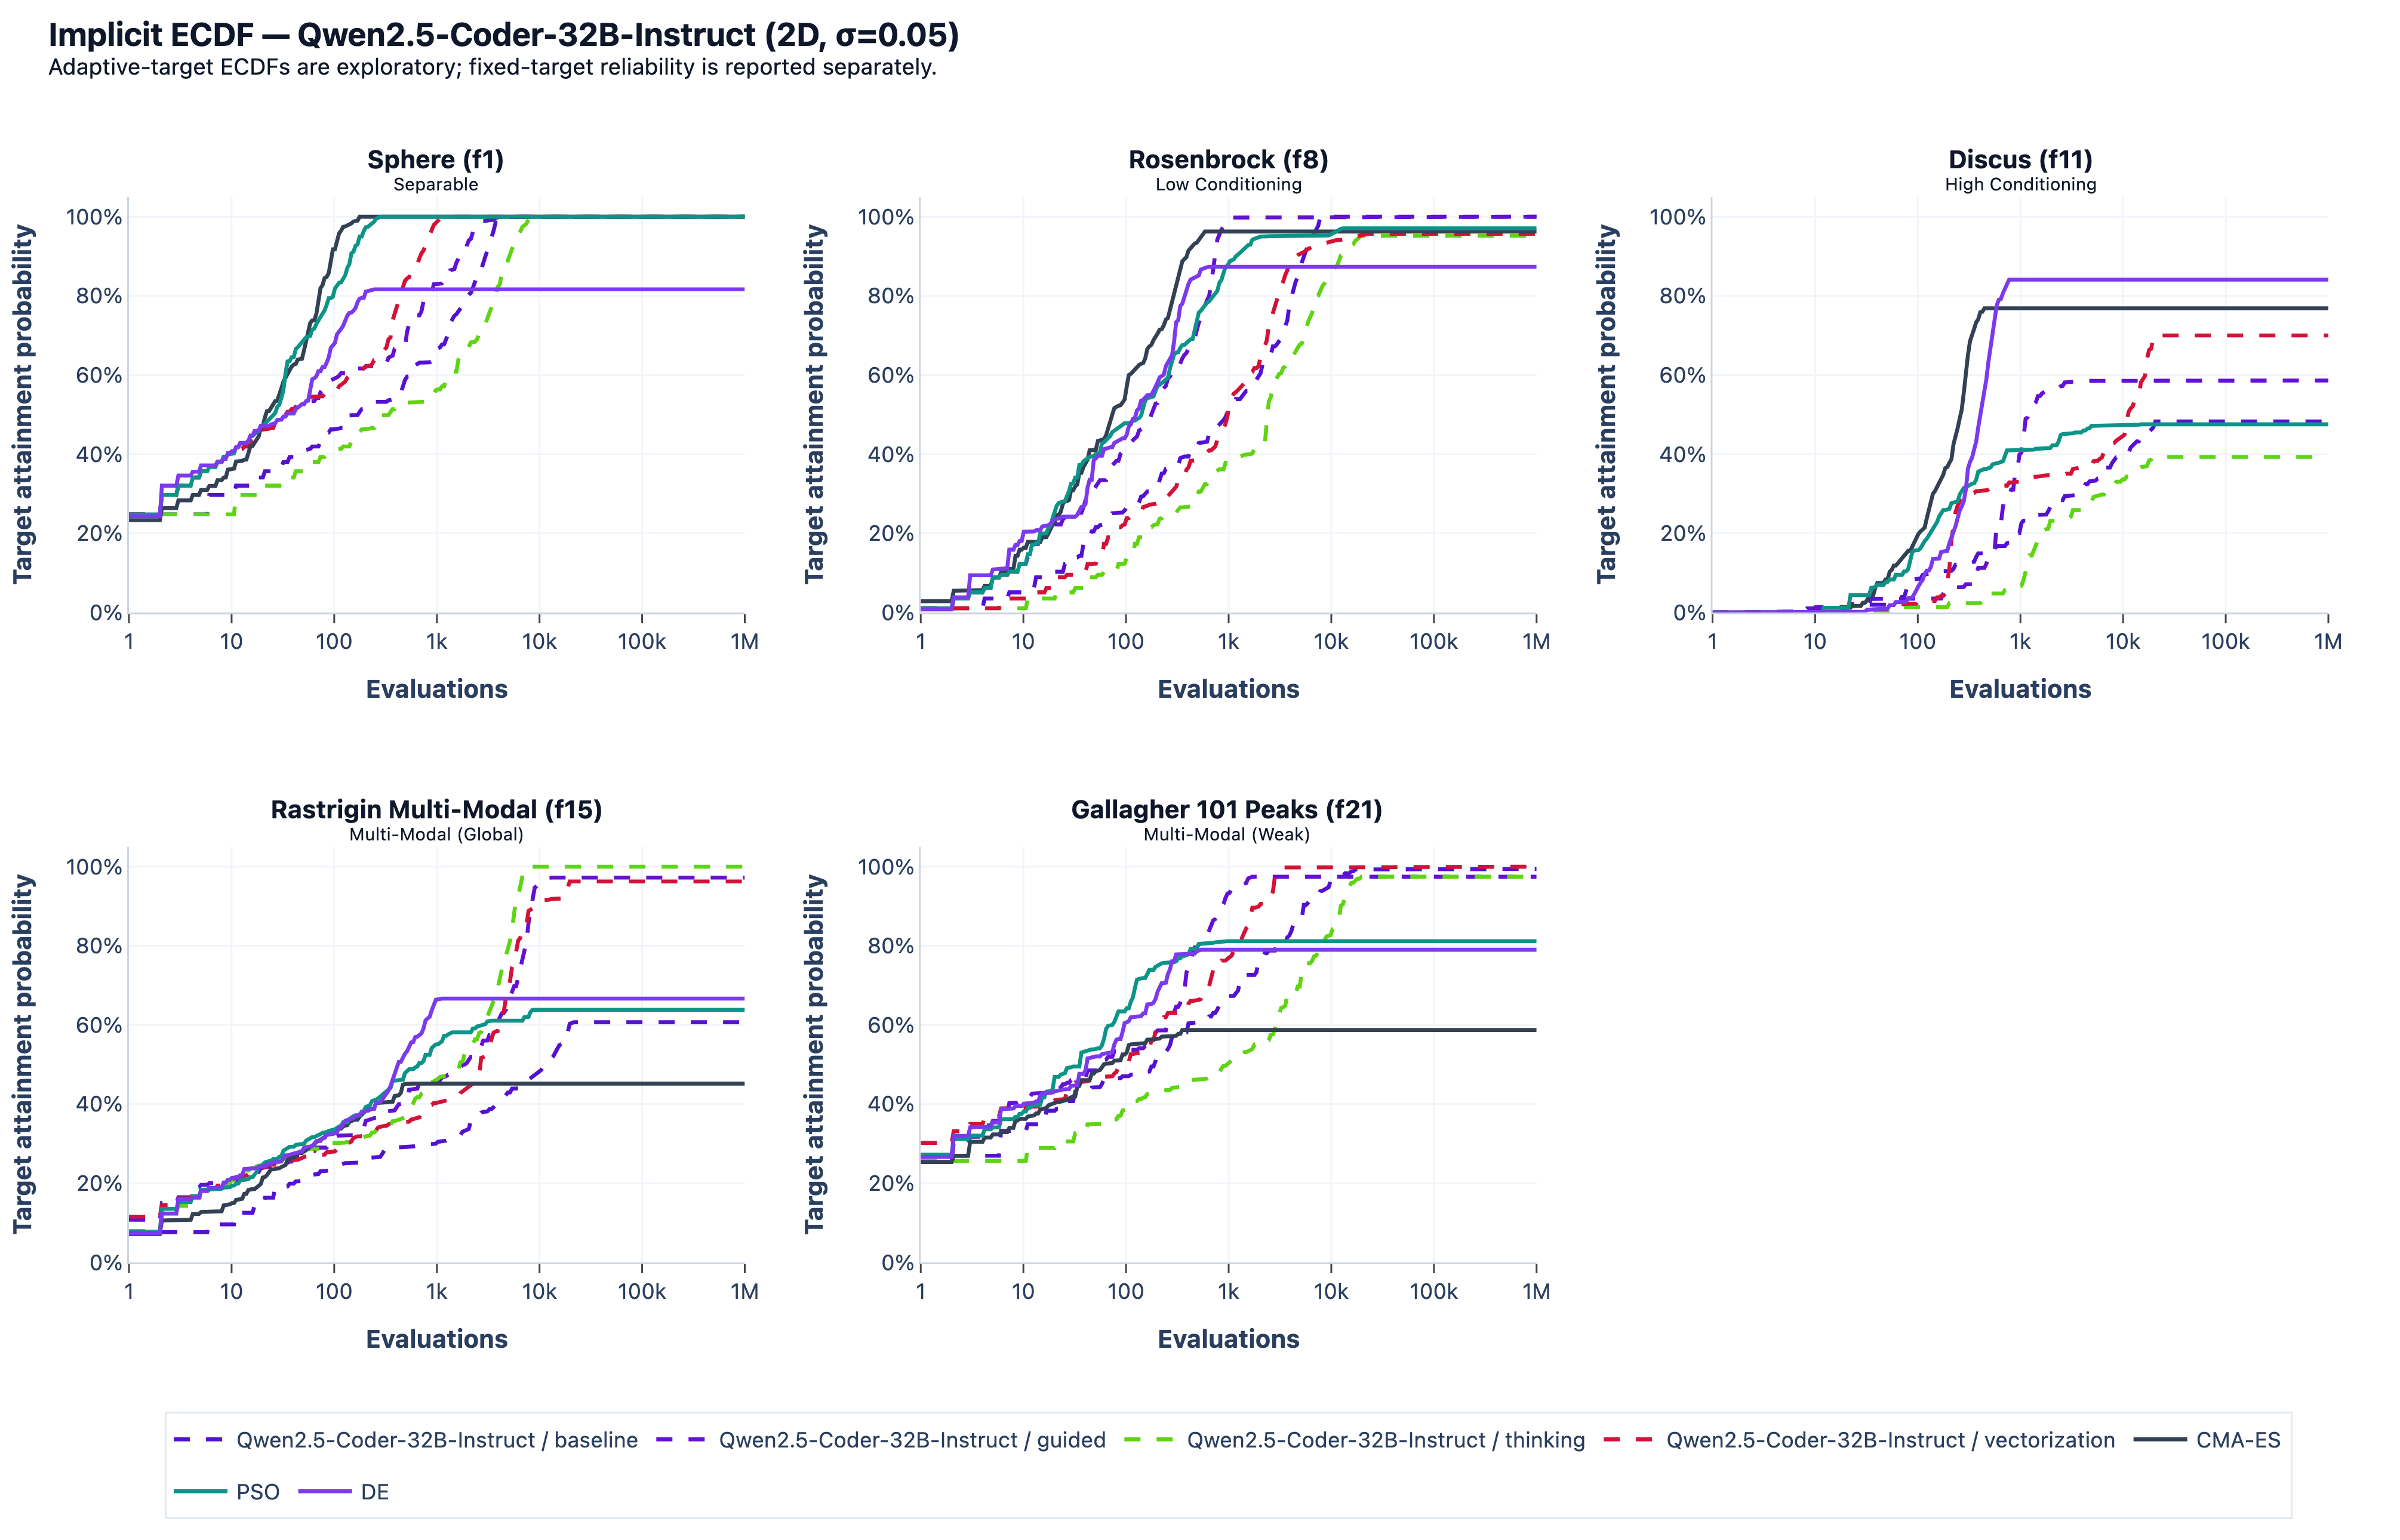
\includegraphics[width=\textwidth,height=0.32\textheight,keepaspectratio]{images/experiments/03_implicit/qwen_32b/2D/std_0.05/target_precision_ecdf.png}
    \caption{Qwen2.5-Coder-32B-Instruct: Implicit, $D=2$,
    $\sigma=0.05$. Convergence (median and IQR) above;
    adaptive target-precision ECDF below. The objective-query allowance
    is 20,000.}
    \label{fig:appendix_03_implicit_qwen_32b_2_std_005}
\end{minipage}
\par\medskip

\par\smallskip\noindent
\begin{minipage}{\linewidth}
    \captionsetup{type=figure,aboveskip=4pt,belowskip=0pt}
    \centering
    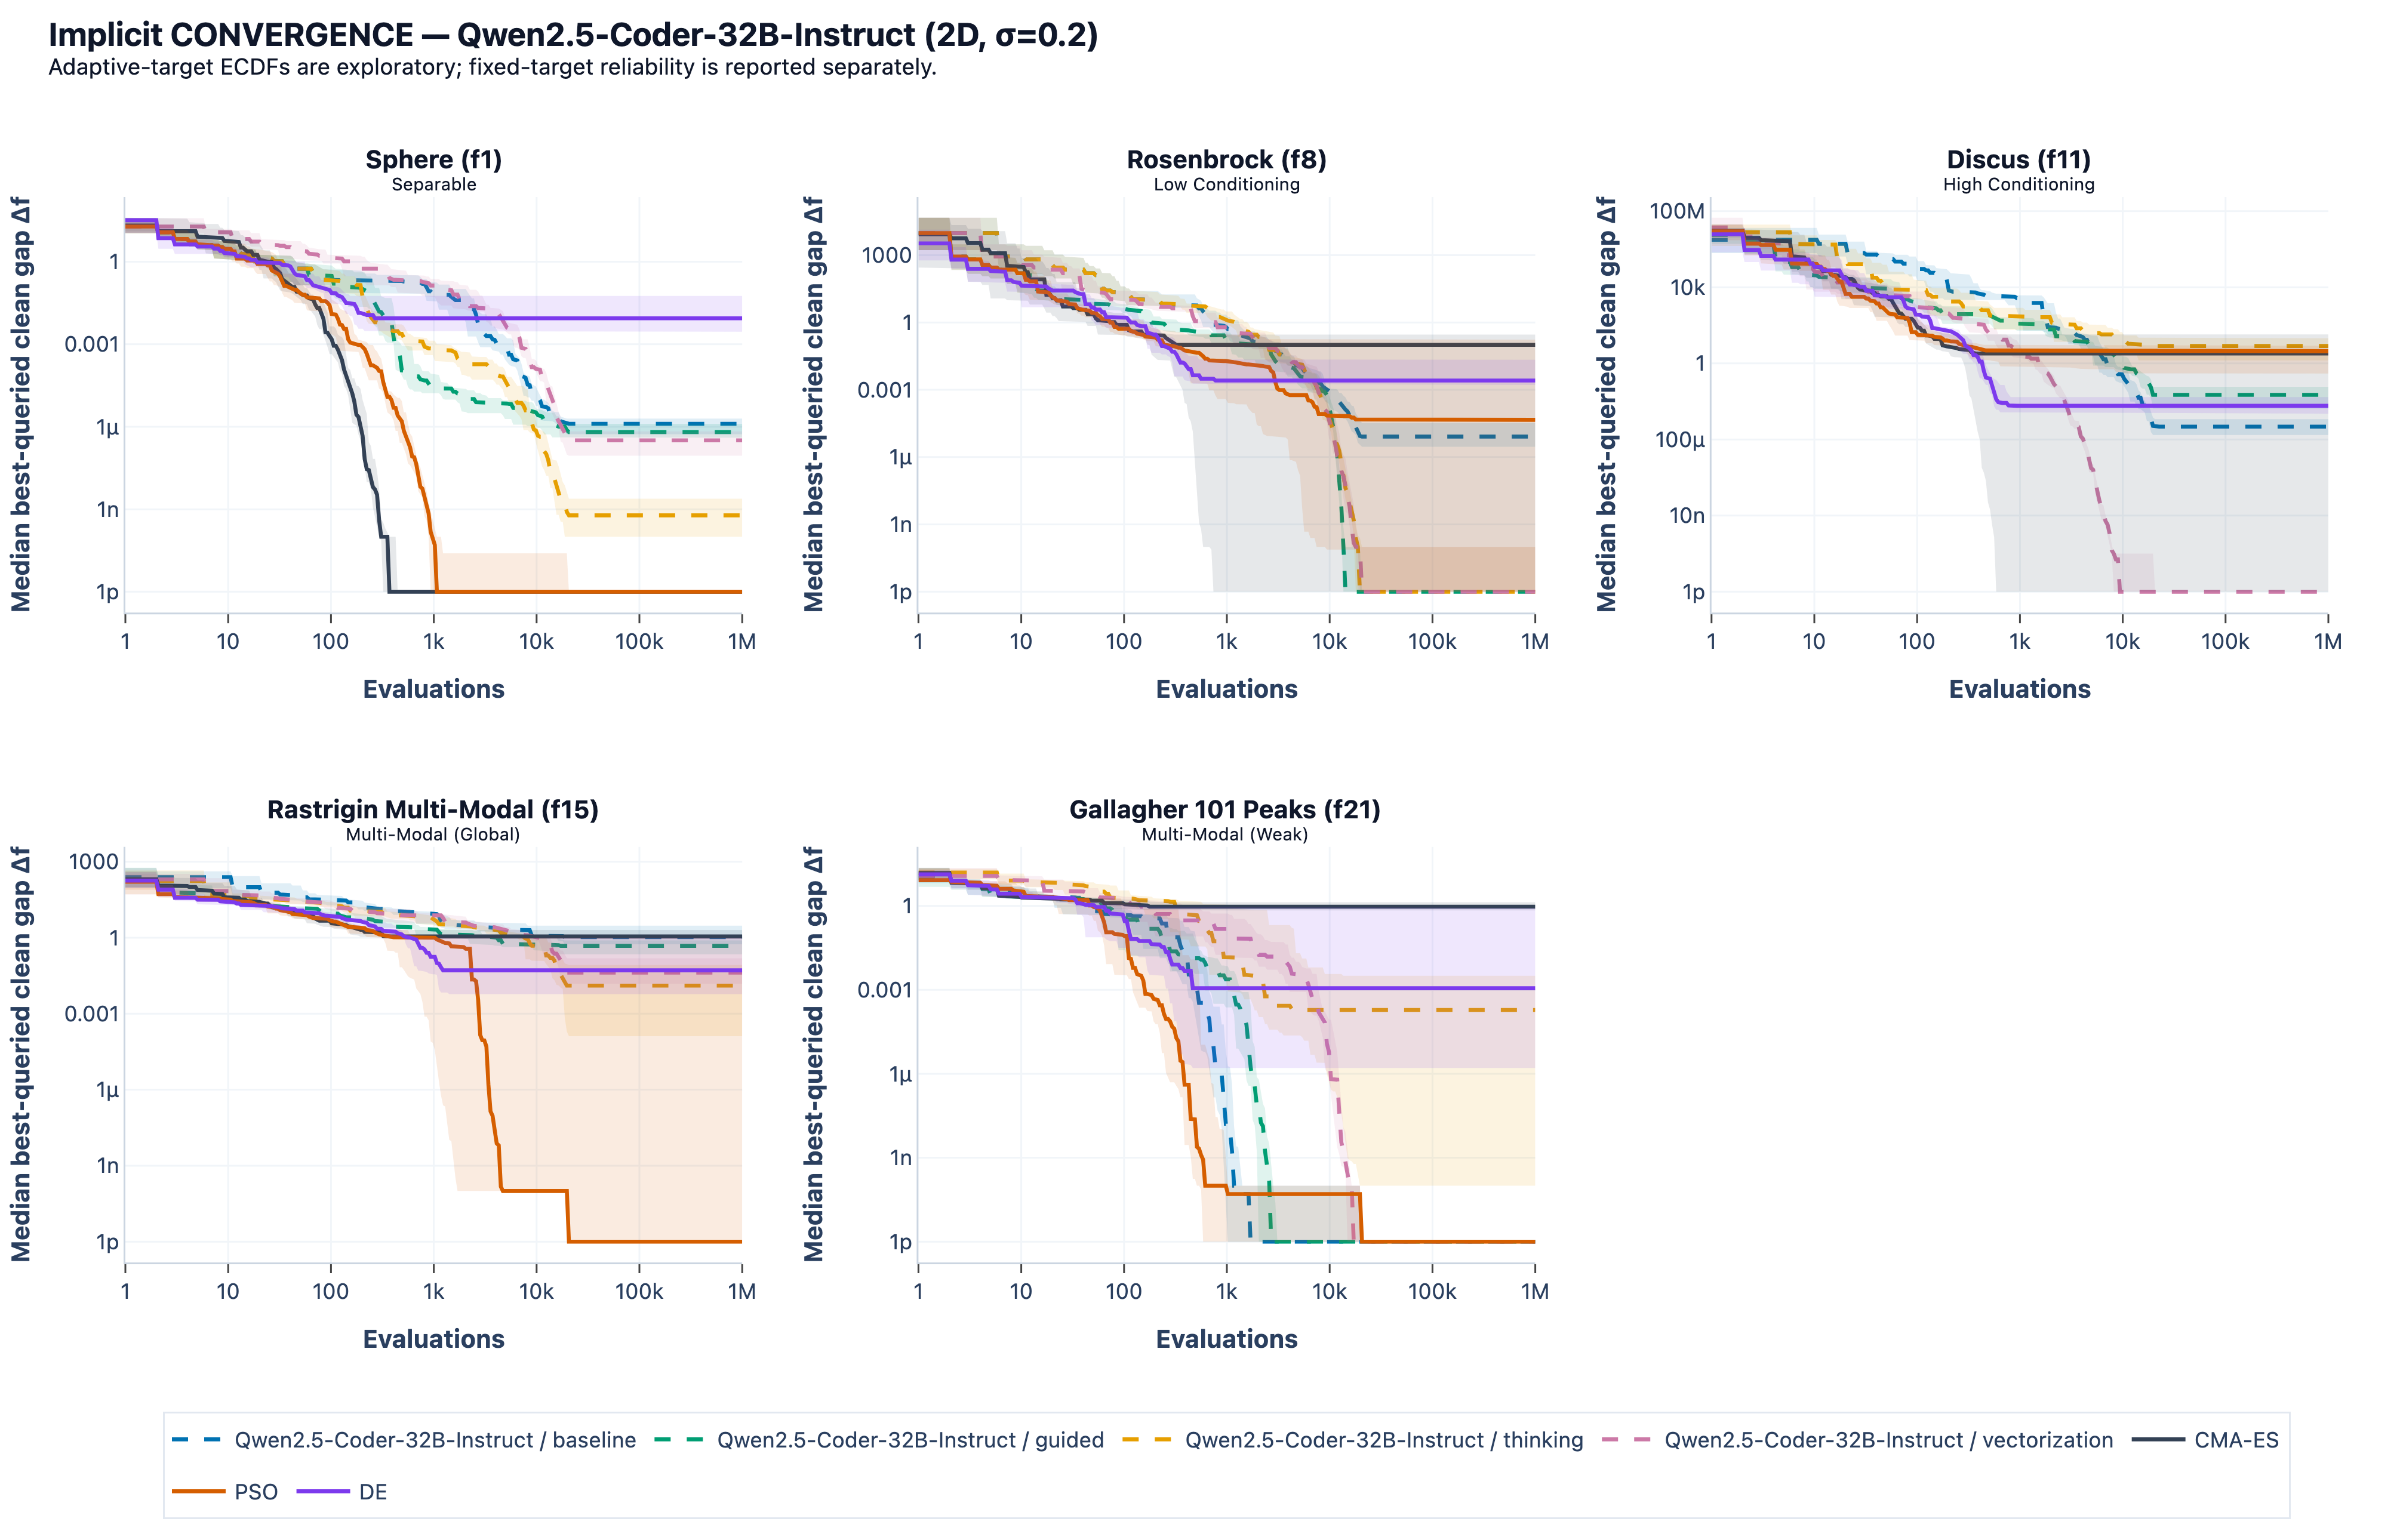
\includegraphics[width=\textwidth,height=0.32\textheight,keepaspectratio]{images/experiments/03_implicit/qwen_32b/2D/std_0.2/convergence_trajectories.png}
    \par\medskip
    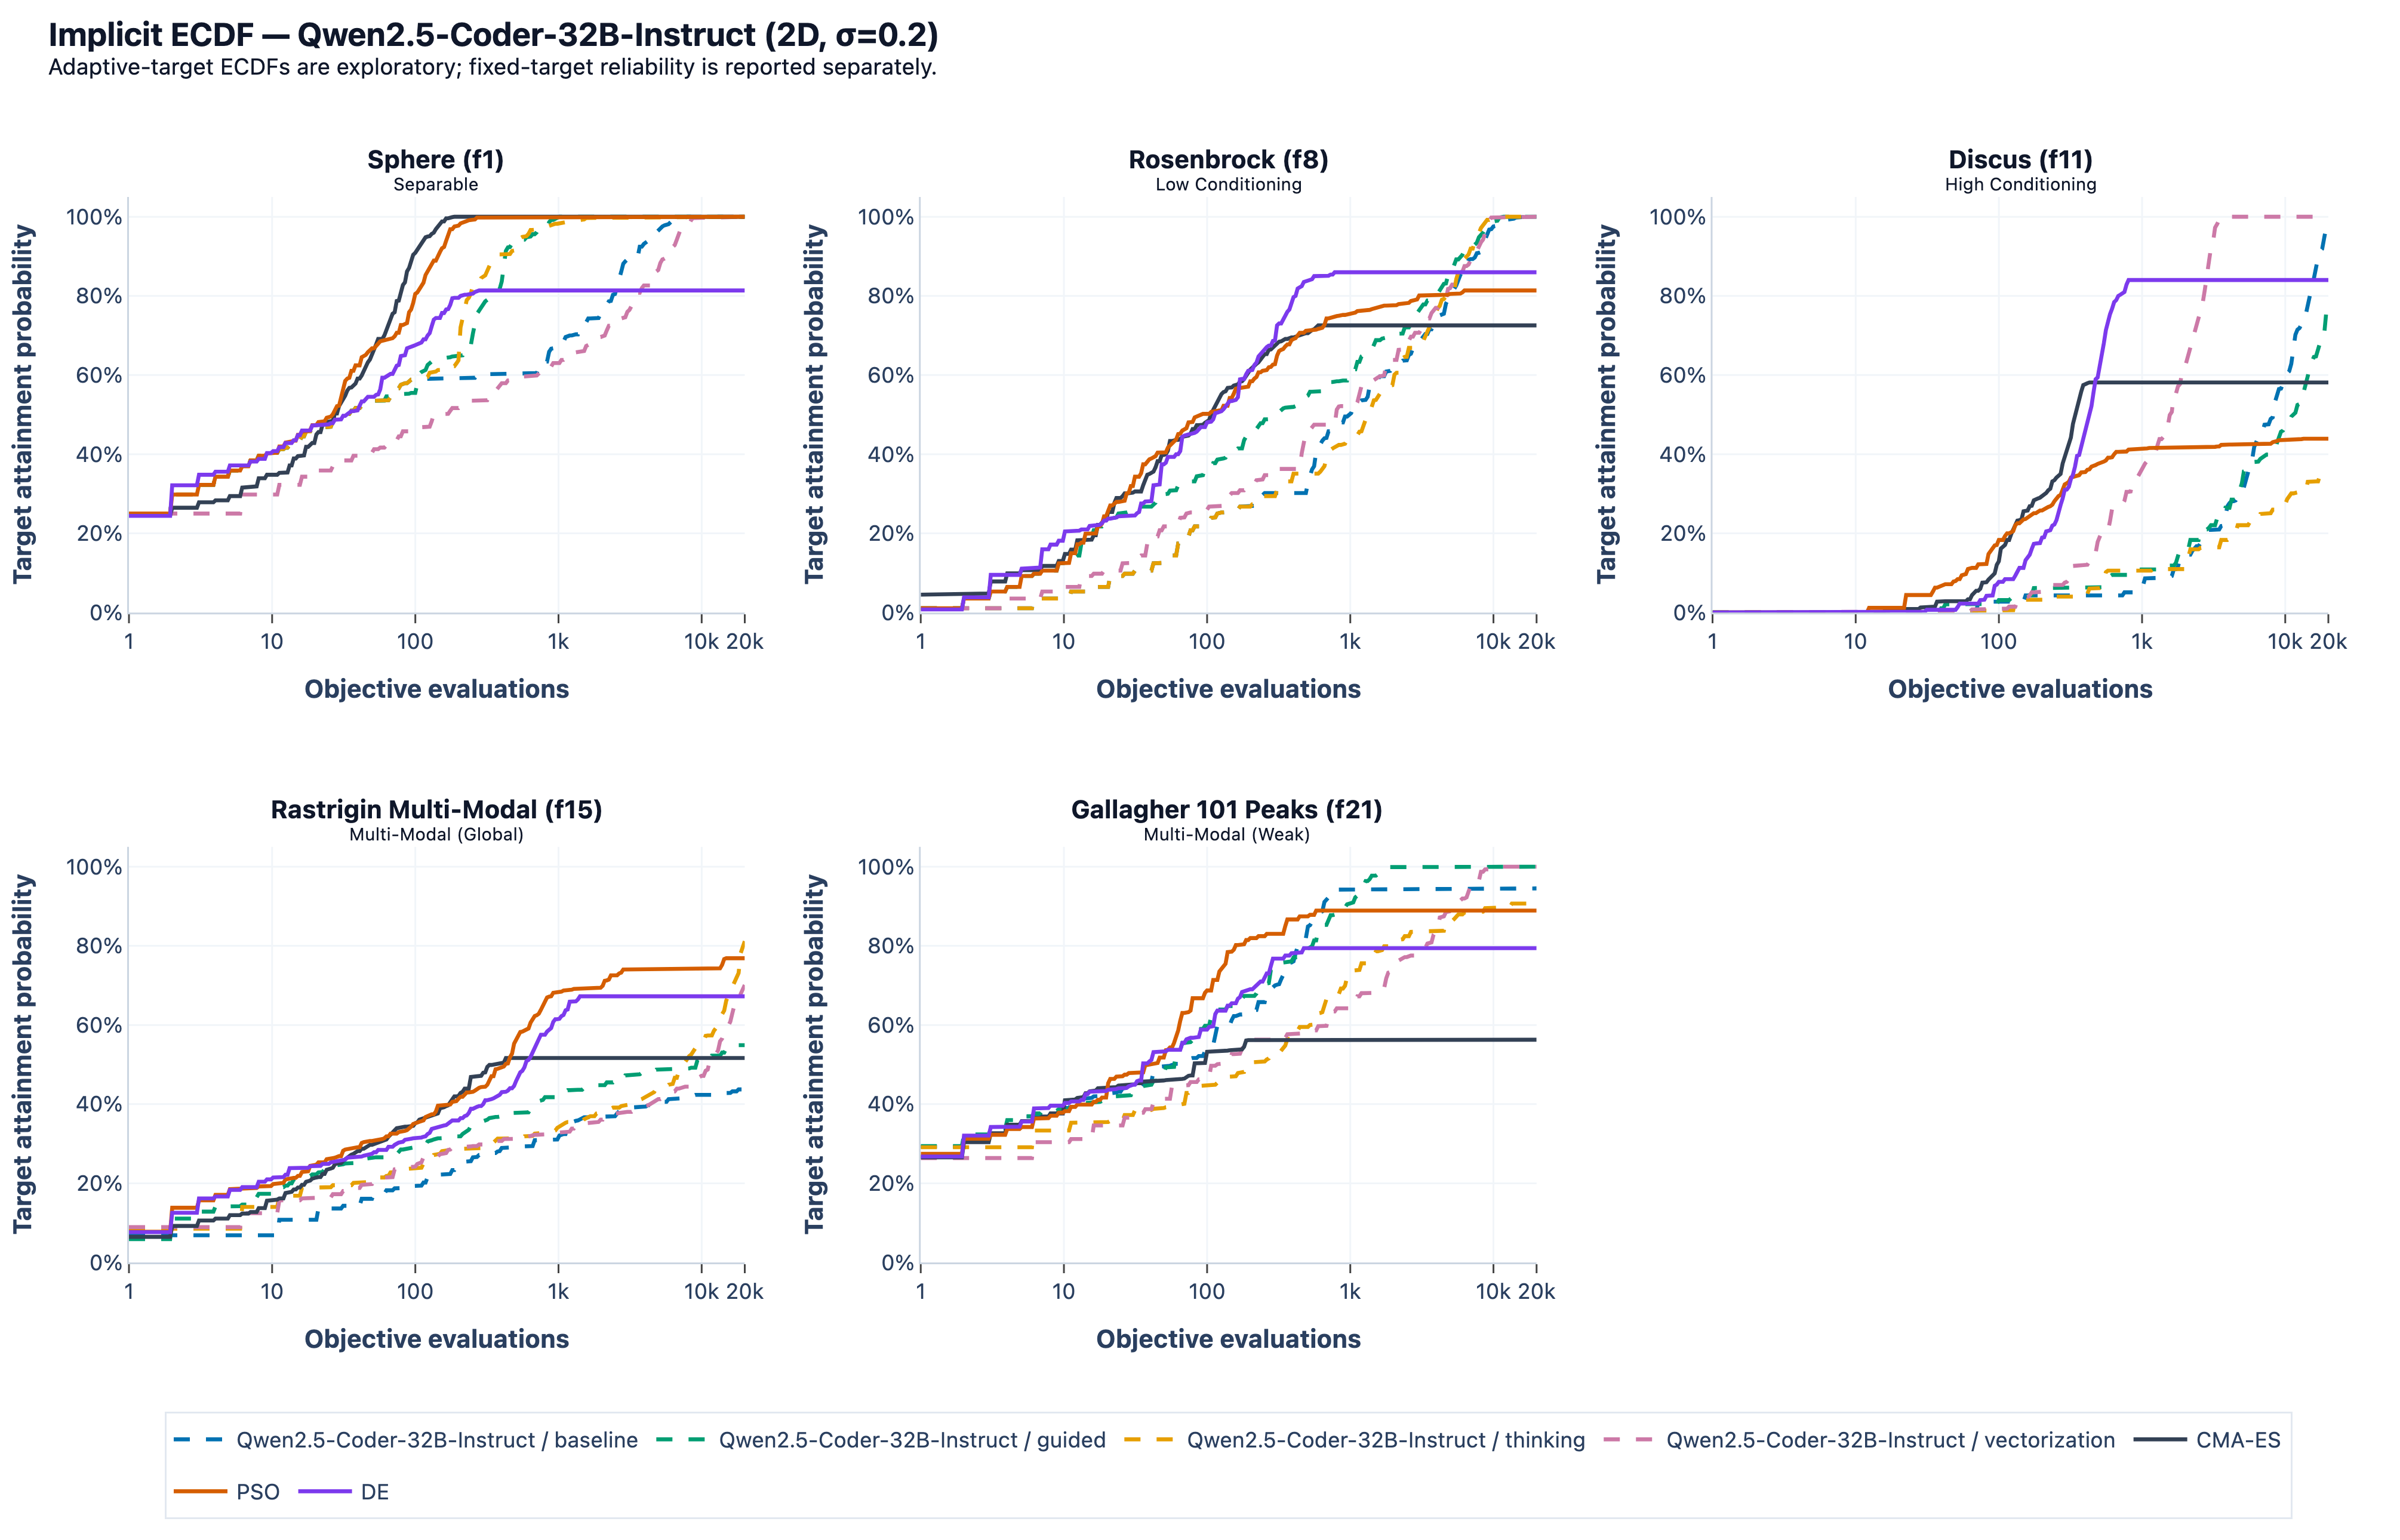
\includegraphics[width=\textwidth,height=0.32\textheight,keepaspectratio]{images/experiments/03_implicit/qwen_32b/2D/std_0.2/target_precision_ecdf.png}
    \caption{Qwen2.5-Coder-32B-Instruct: Implicit, $D=2$,
    $\sigma=0.2$. Convergence (median and IQR) above;
    adaptive target-precision ECDF below. The objective-query allowance
    is 20,000.}
    \label{fig:appendix_03_implicit_qwen_32b_2_std_02}
\end{minipage}
\par\medskip

\par\smallskip\noindent
\begin{minipage}{\linewidth}
    \captionsetup{type=figure,aboveskip=4pt,belowskip=0pt}
    \centering
    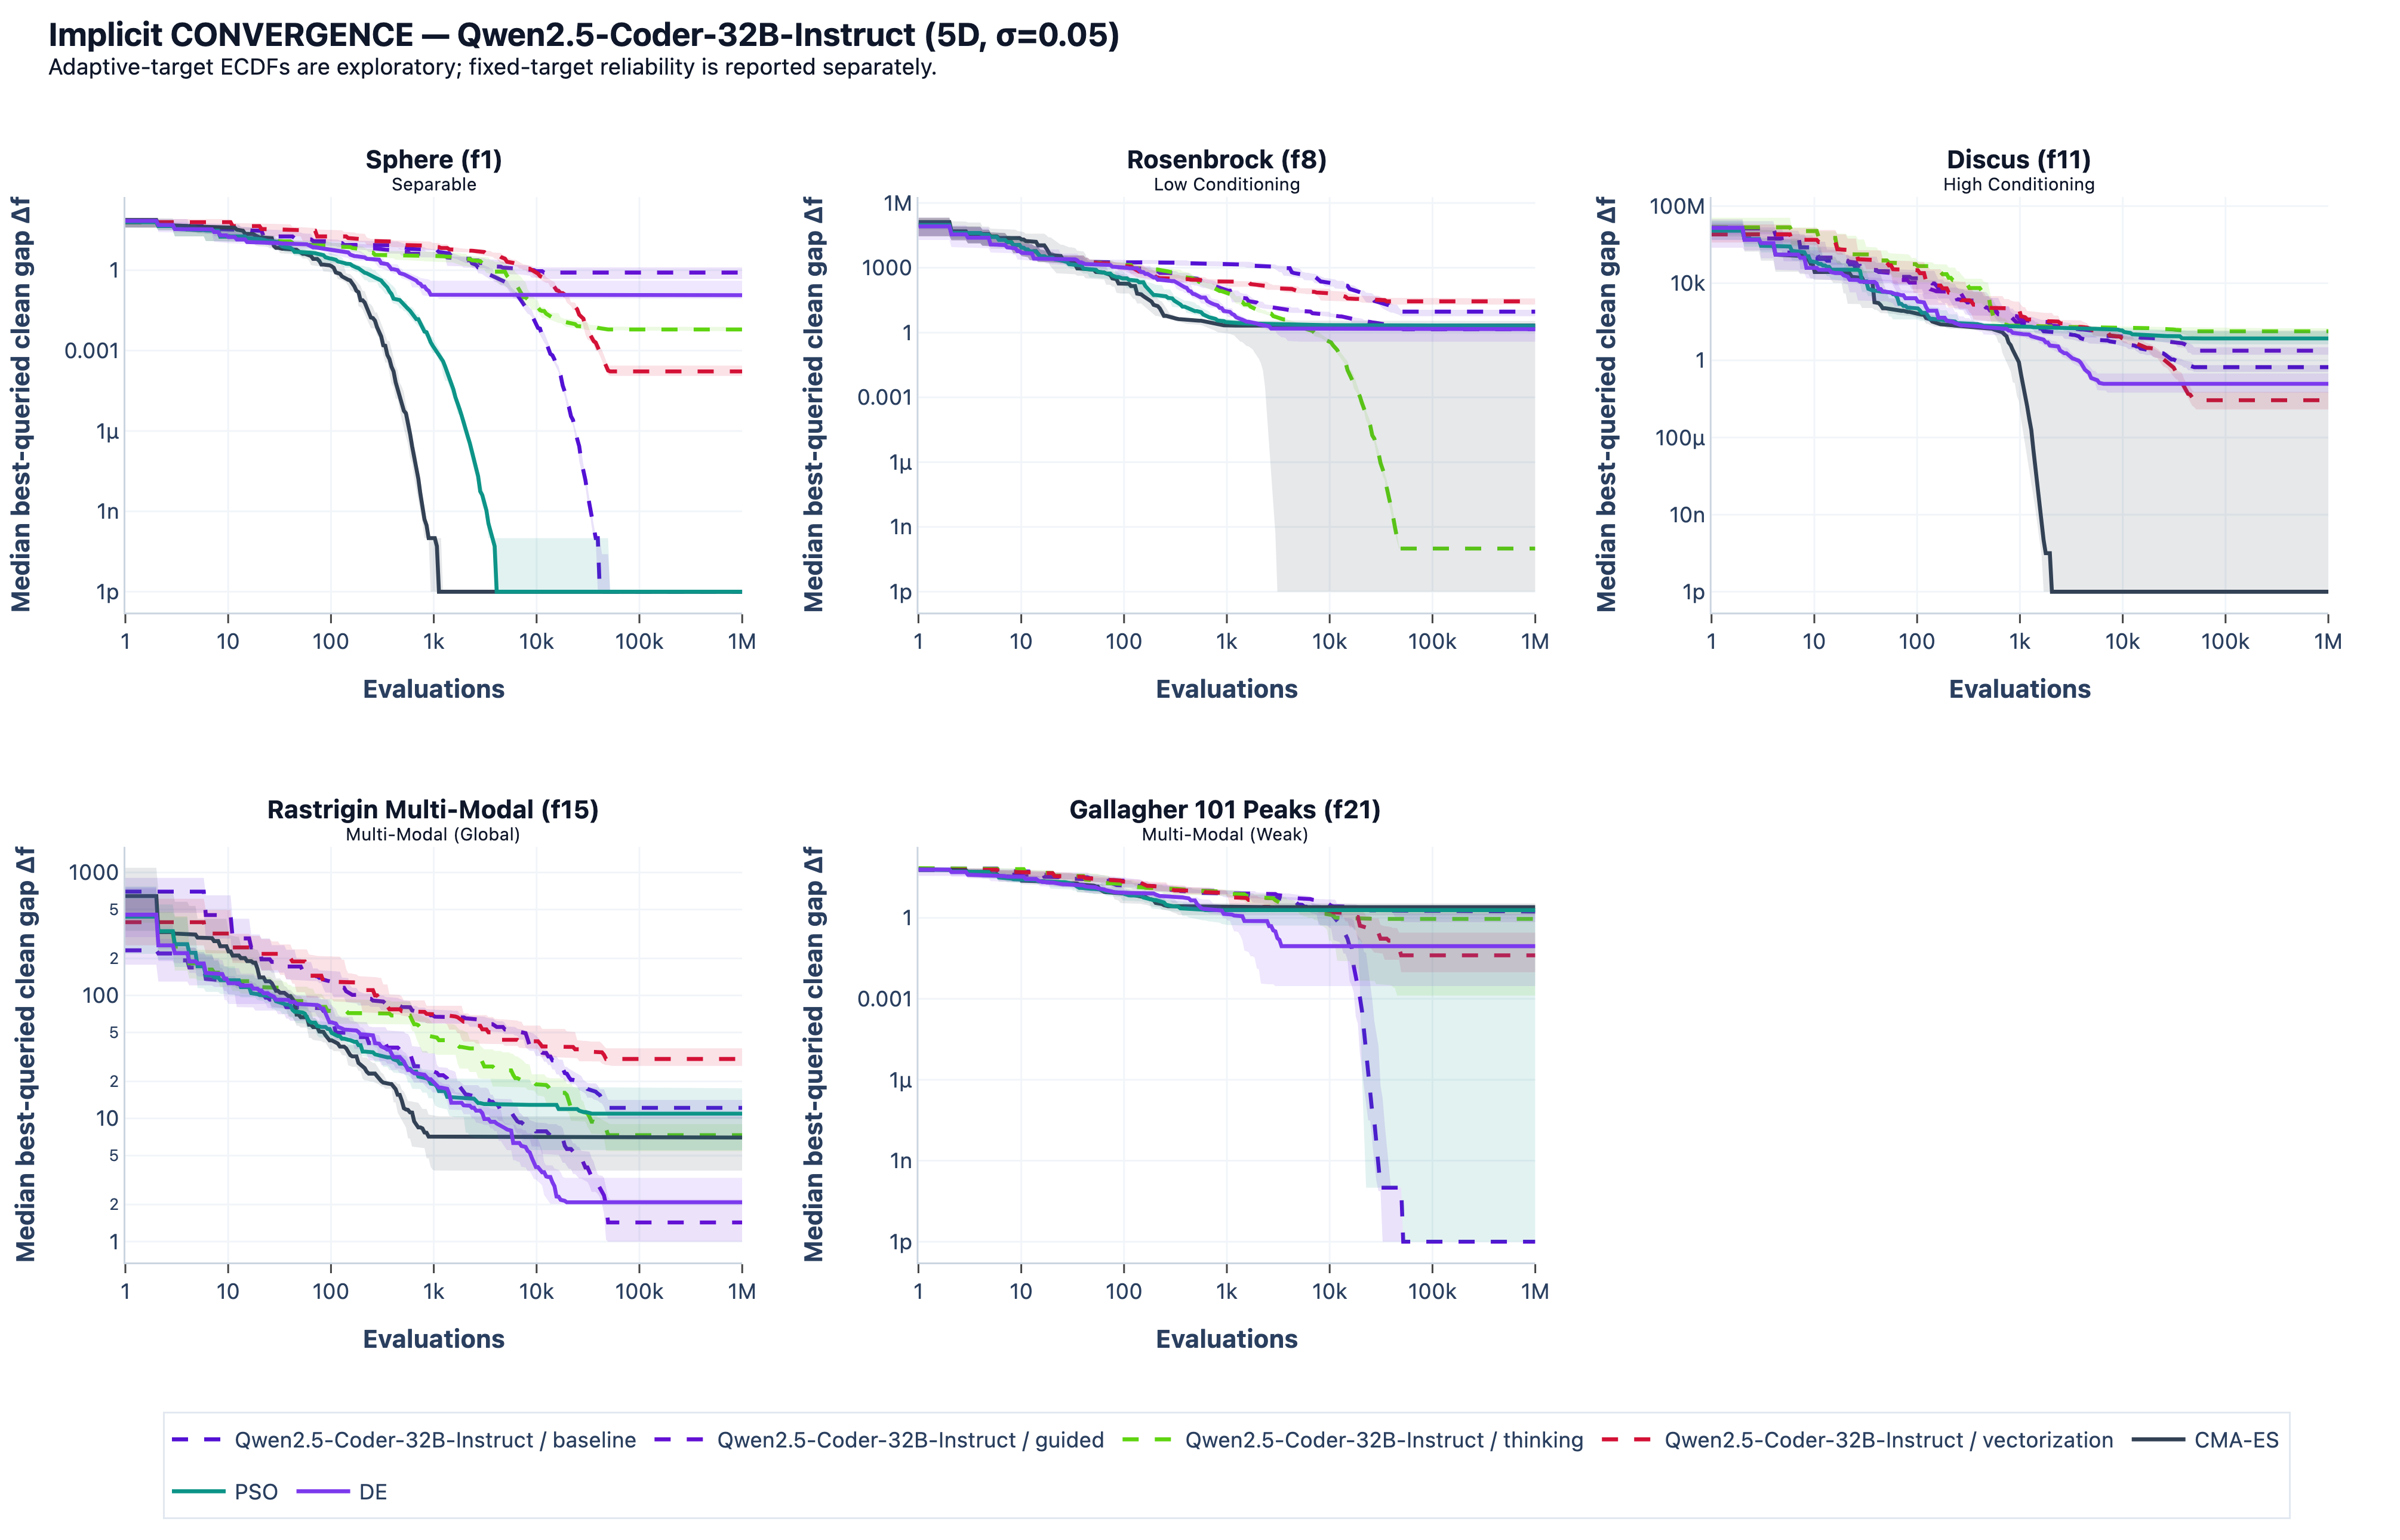
\includegraphics[width=\textwidth,height=0.32\textheight,keepaspectratio]{images/experiments/03_implicit/qwen_32b/5D/std_0.05/convergence_trajectories.png}
    \par\medskip
    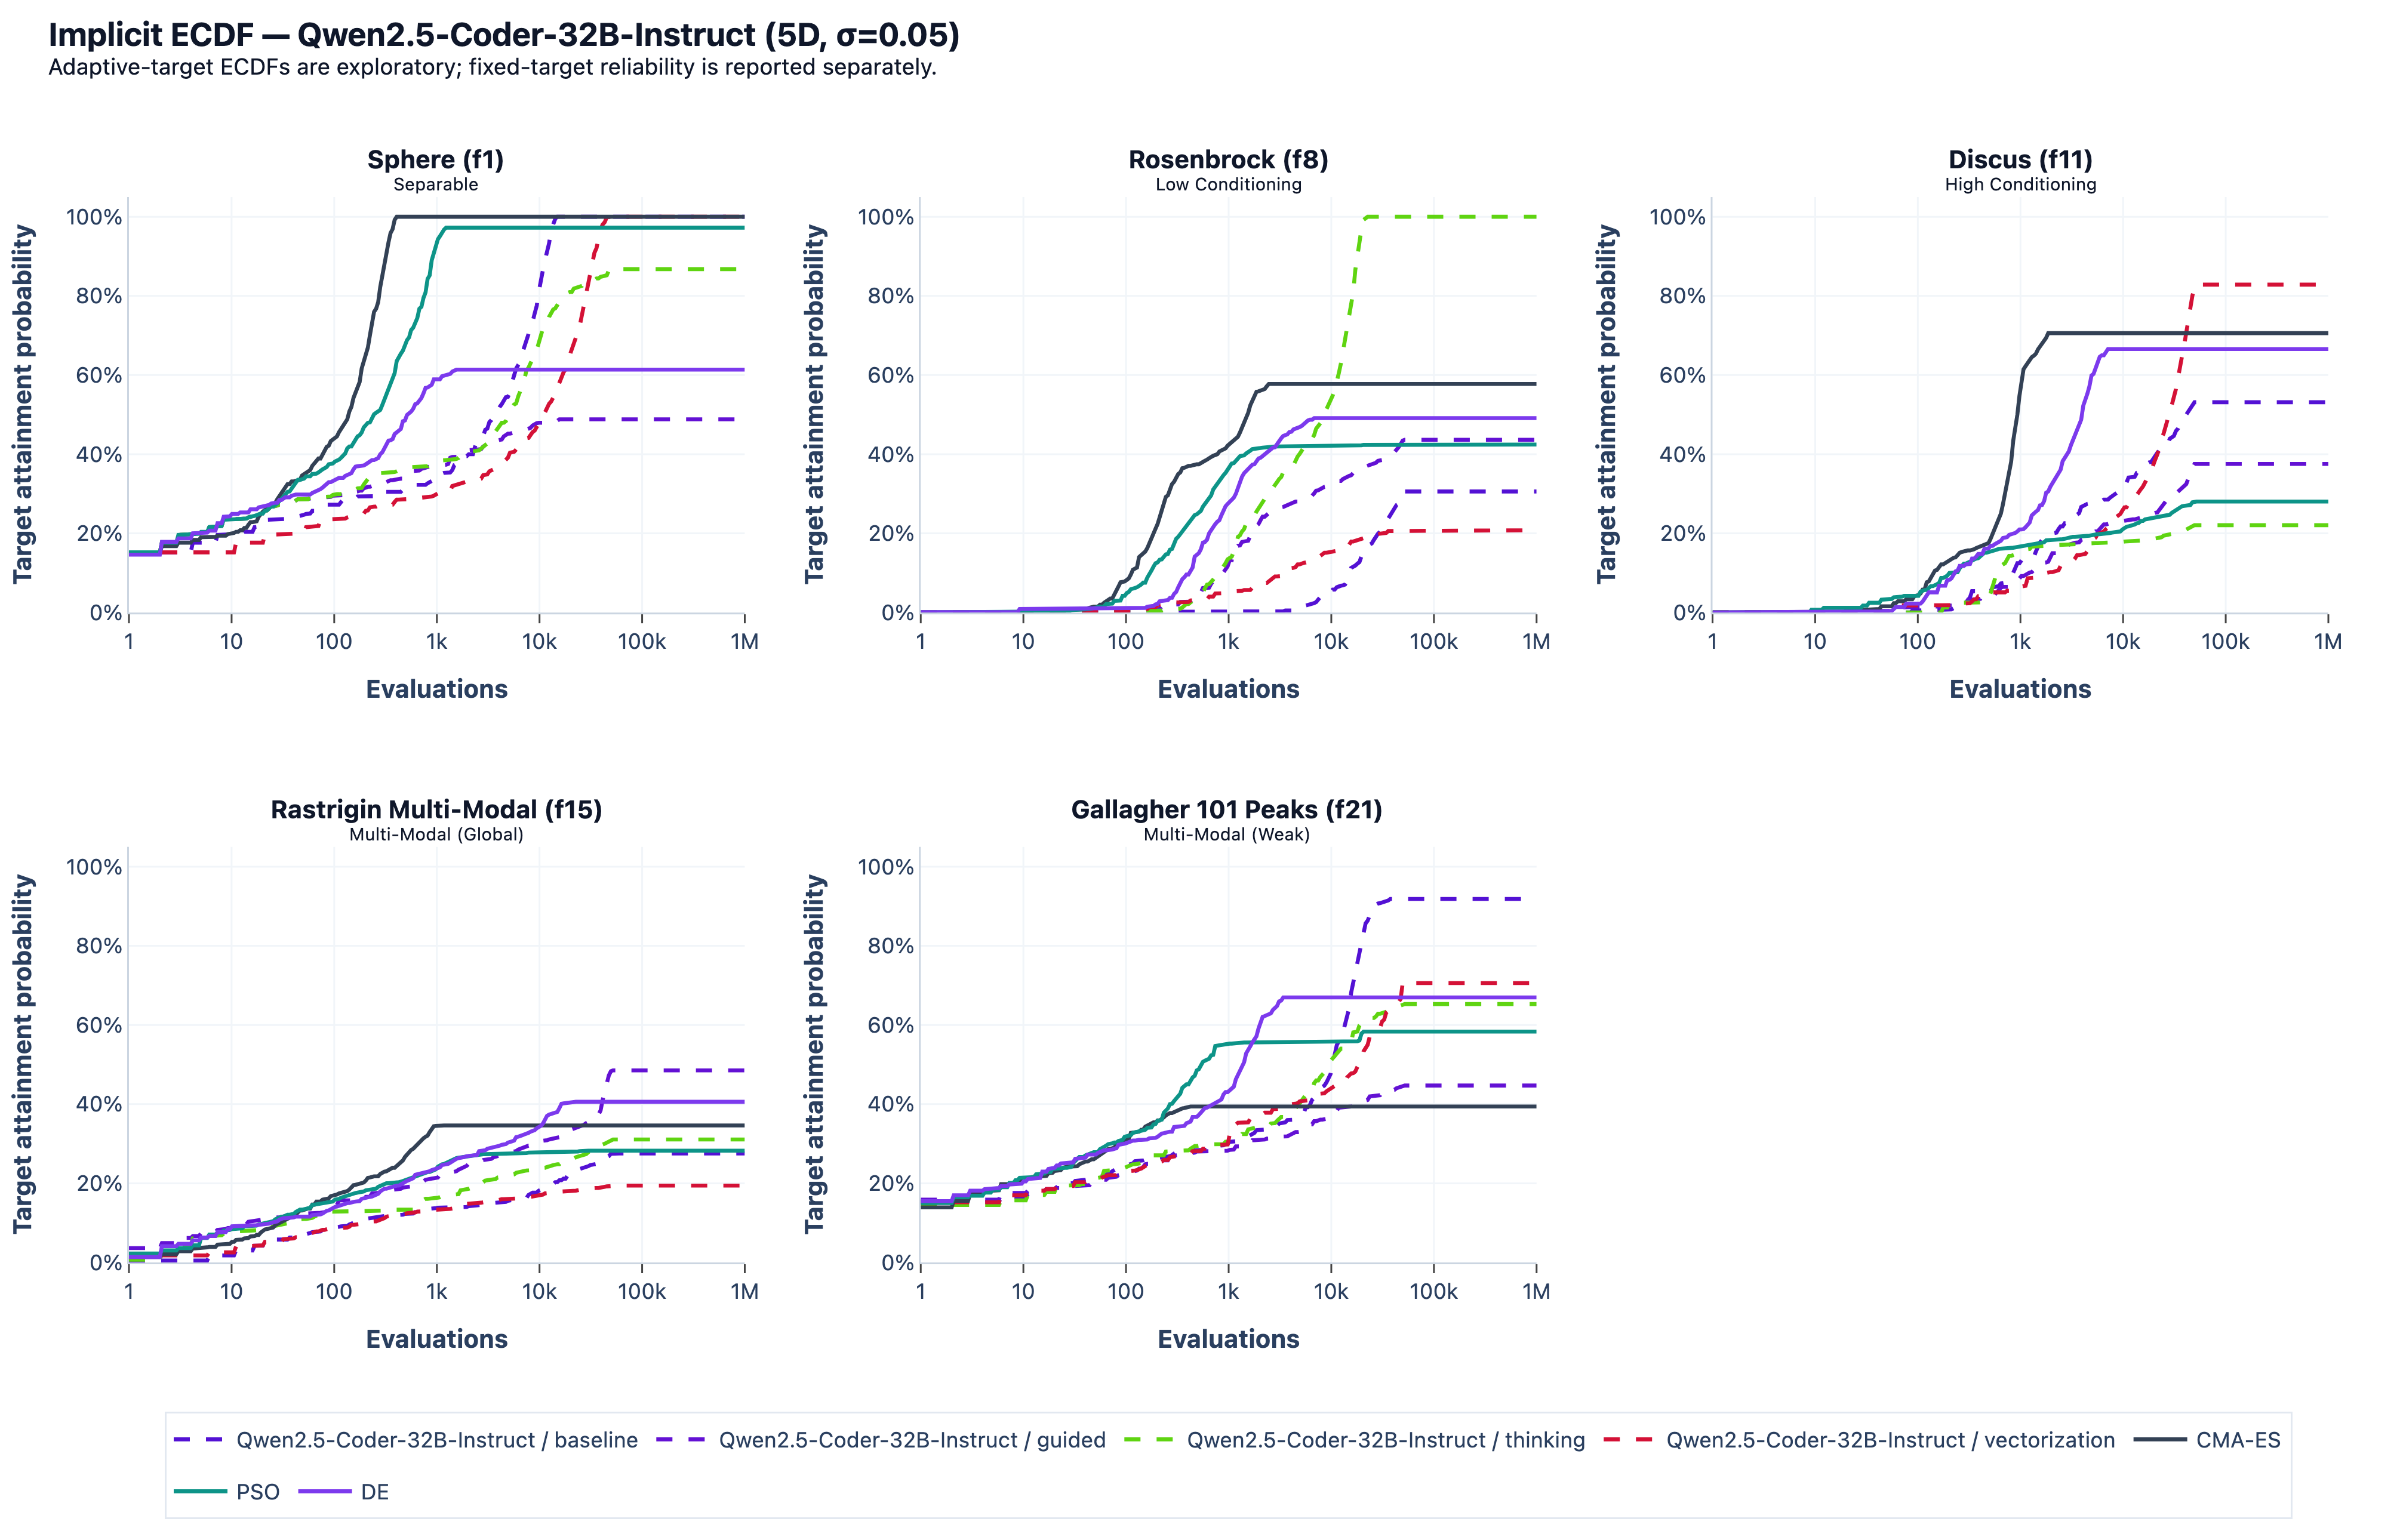
\includegraphics[width=\textwidth,height=0.32\textheight,keepaspectratio]{images/experiments/03_implicit/qwen_32b/5D/std_0.05/target_precision_ecdf.png}
    \caption{Qwen2.5-Coder-32B-Instruct: Implicit, $D=5$,
    $\sigma=0.05$. Convergence (median and IQR) above;
    adaptive target-precision ECDF below. The objective-query allowance
    is 50,000.}
    \label{fig:appendix_03_implicit_qwen_32b_5_std_005}
\end{minipage}
\par\medskip

\subsection{DeepSeek-Coder-V2-Lite-Instruct}
\nopagebreak[4]

\par\smallskip\noindent
\begin{minipage}{\linewidth}
    \captionsetup{type=figure,aboveskip=4pt,belowskip=0pt}
    \centering
    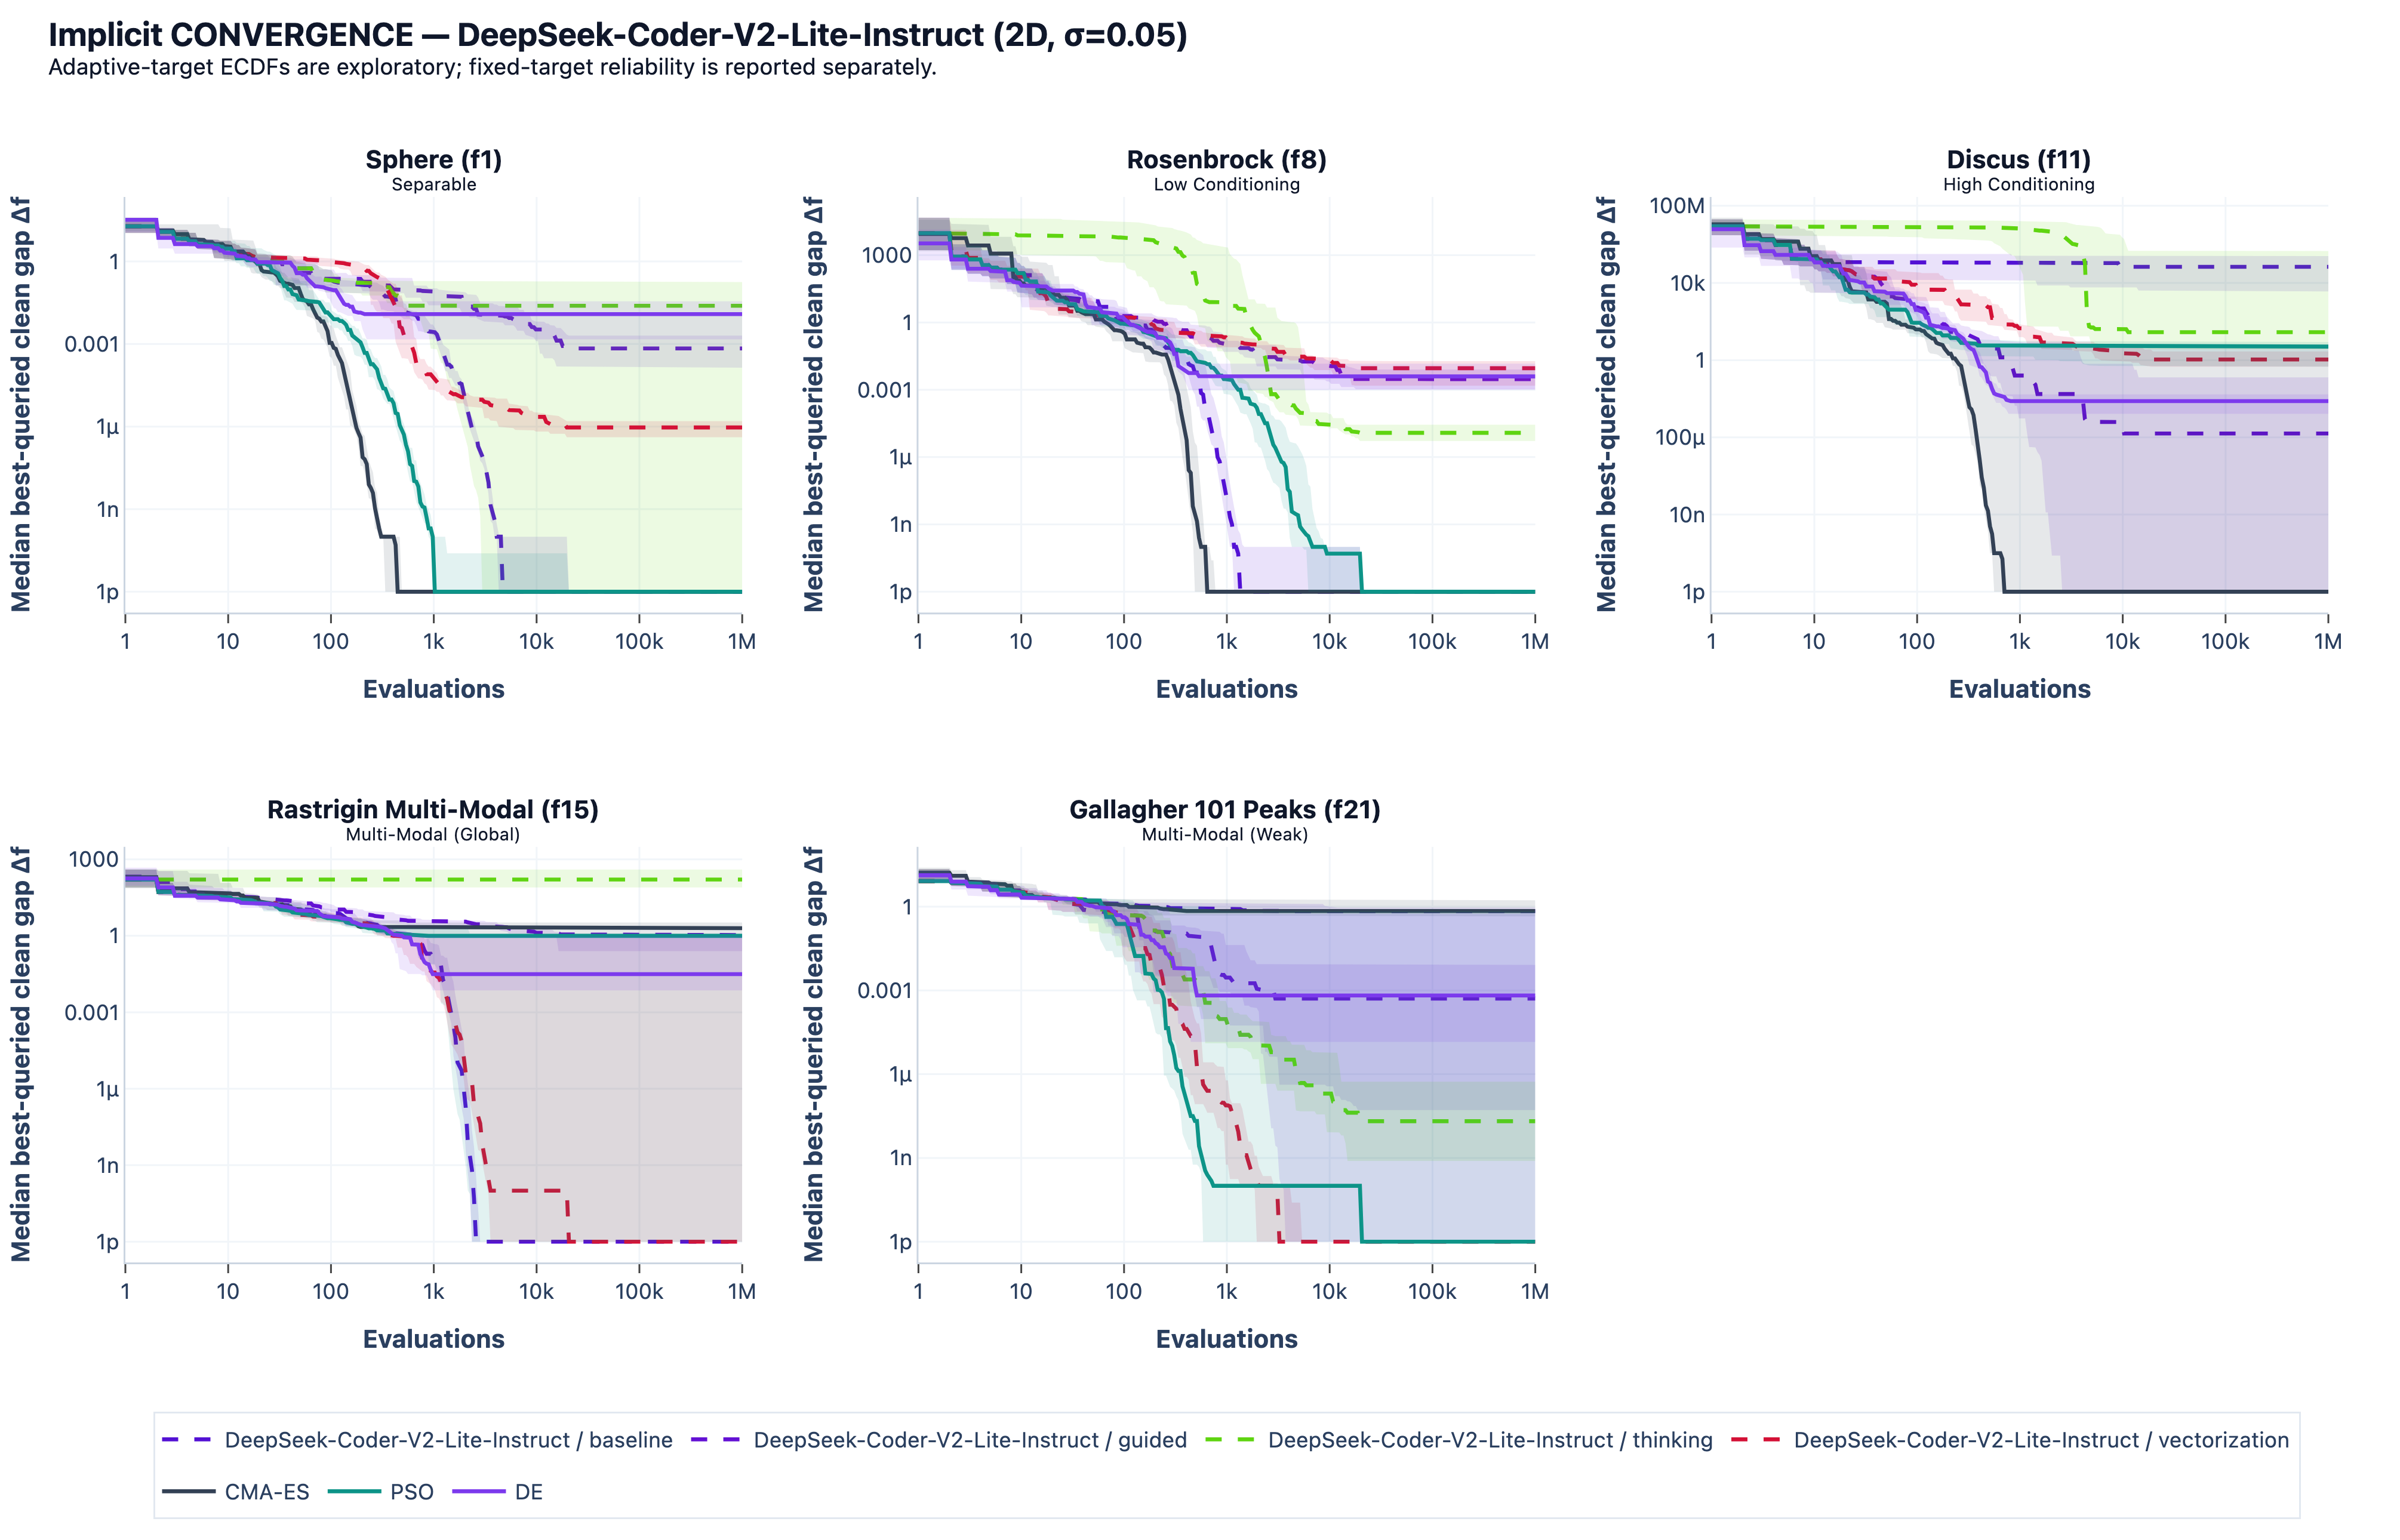
\includegraphics[width=\textwidth,height=0.32\textheight,keepaspectratio]{images/experiments/03_implicit/deepseek_coder_v2_lite_instruct_q4_k_m/2D/std_0.05/convergence_trajectories.png}
    \par\medskip
    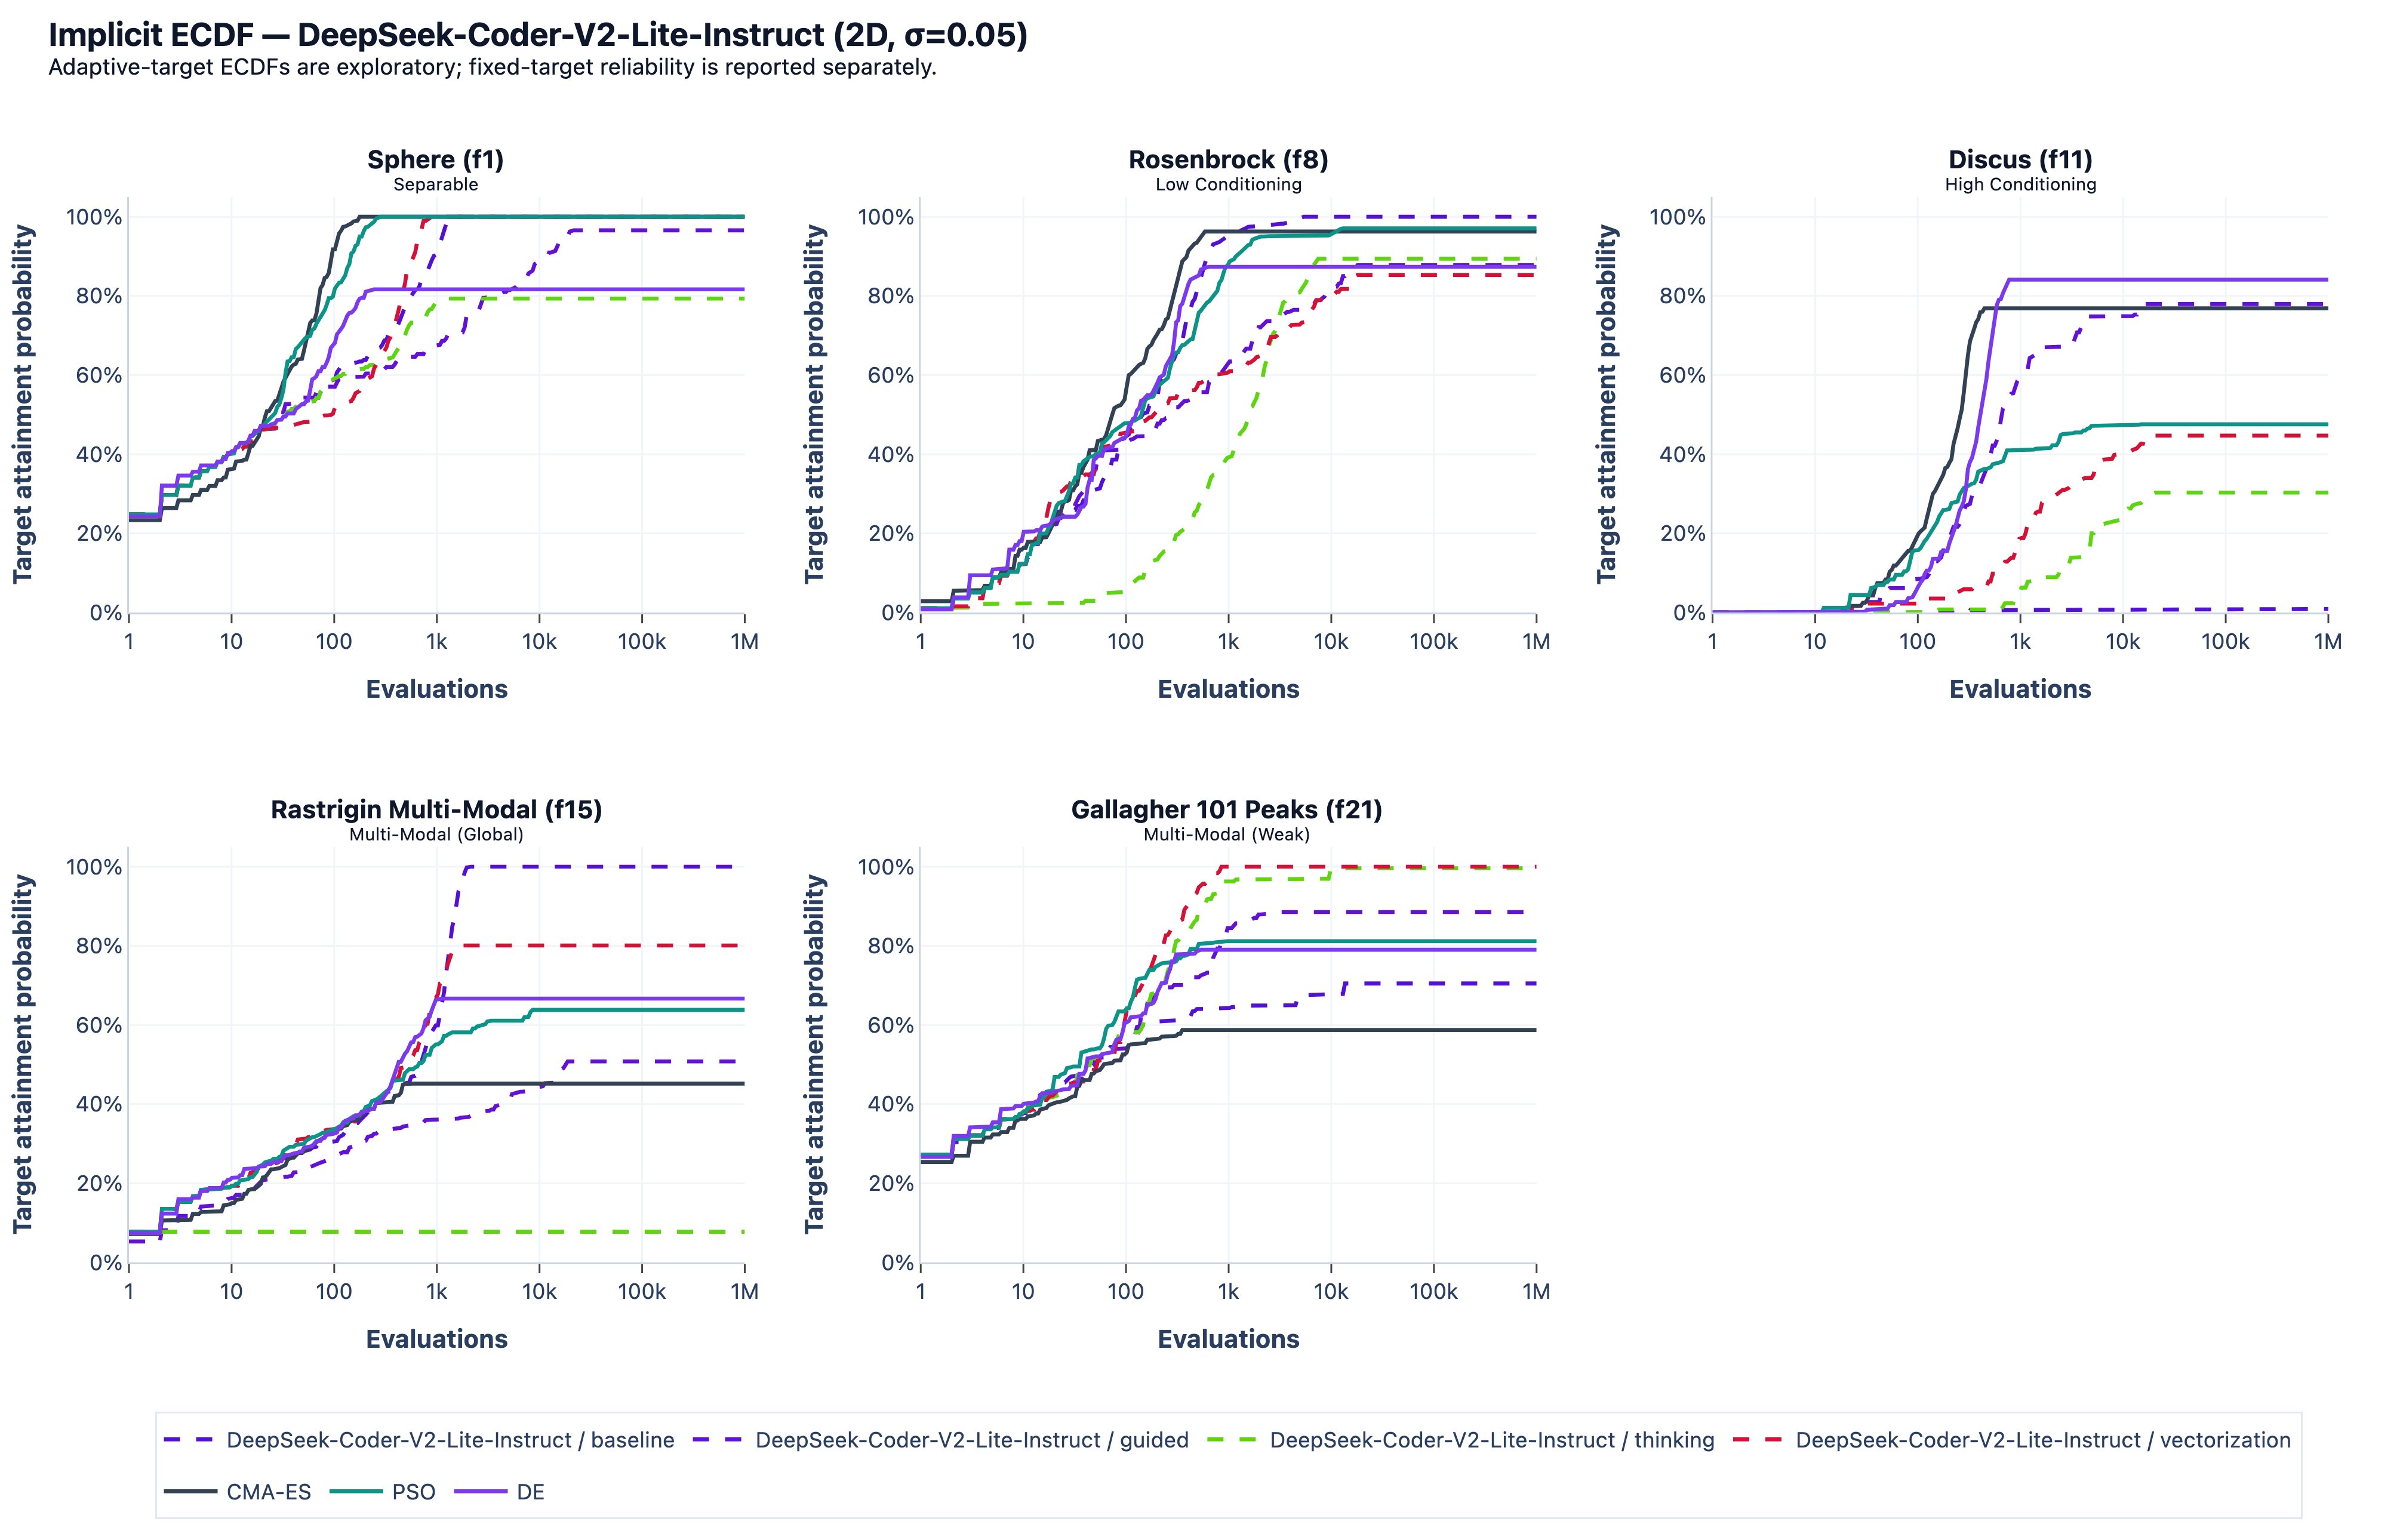
\includegraphics[width=\textwidth,height=0.32\textheight,keepaspectratio]{images/experiments/03_implicit/deepseek_coder_v2_lite_instruct_q4_k_m/2D/std_0.05/target_precision_ecdf.png}
    \caption{DeepSeek-Coder-V2-Lite-Instruct: Implicit, $D=2$,
    $\sigma=0.05$. Convergence (median and IQR) above;
    adaptive target-precision ECDF below. The objective-query allowance
    is 20,000.}
    \label{fig:appendix_03_implicit_deepseek_coder_v2_lite_instruct_q4_k_m_2_std_005}
\end{minipage}
\par\medskip

\par\smallskip\noindent
\begin{minipage}{\linewidth}
    \captionsetup{type=figure,aboveskip=4pt,belowskip=0pt}
    \centering
    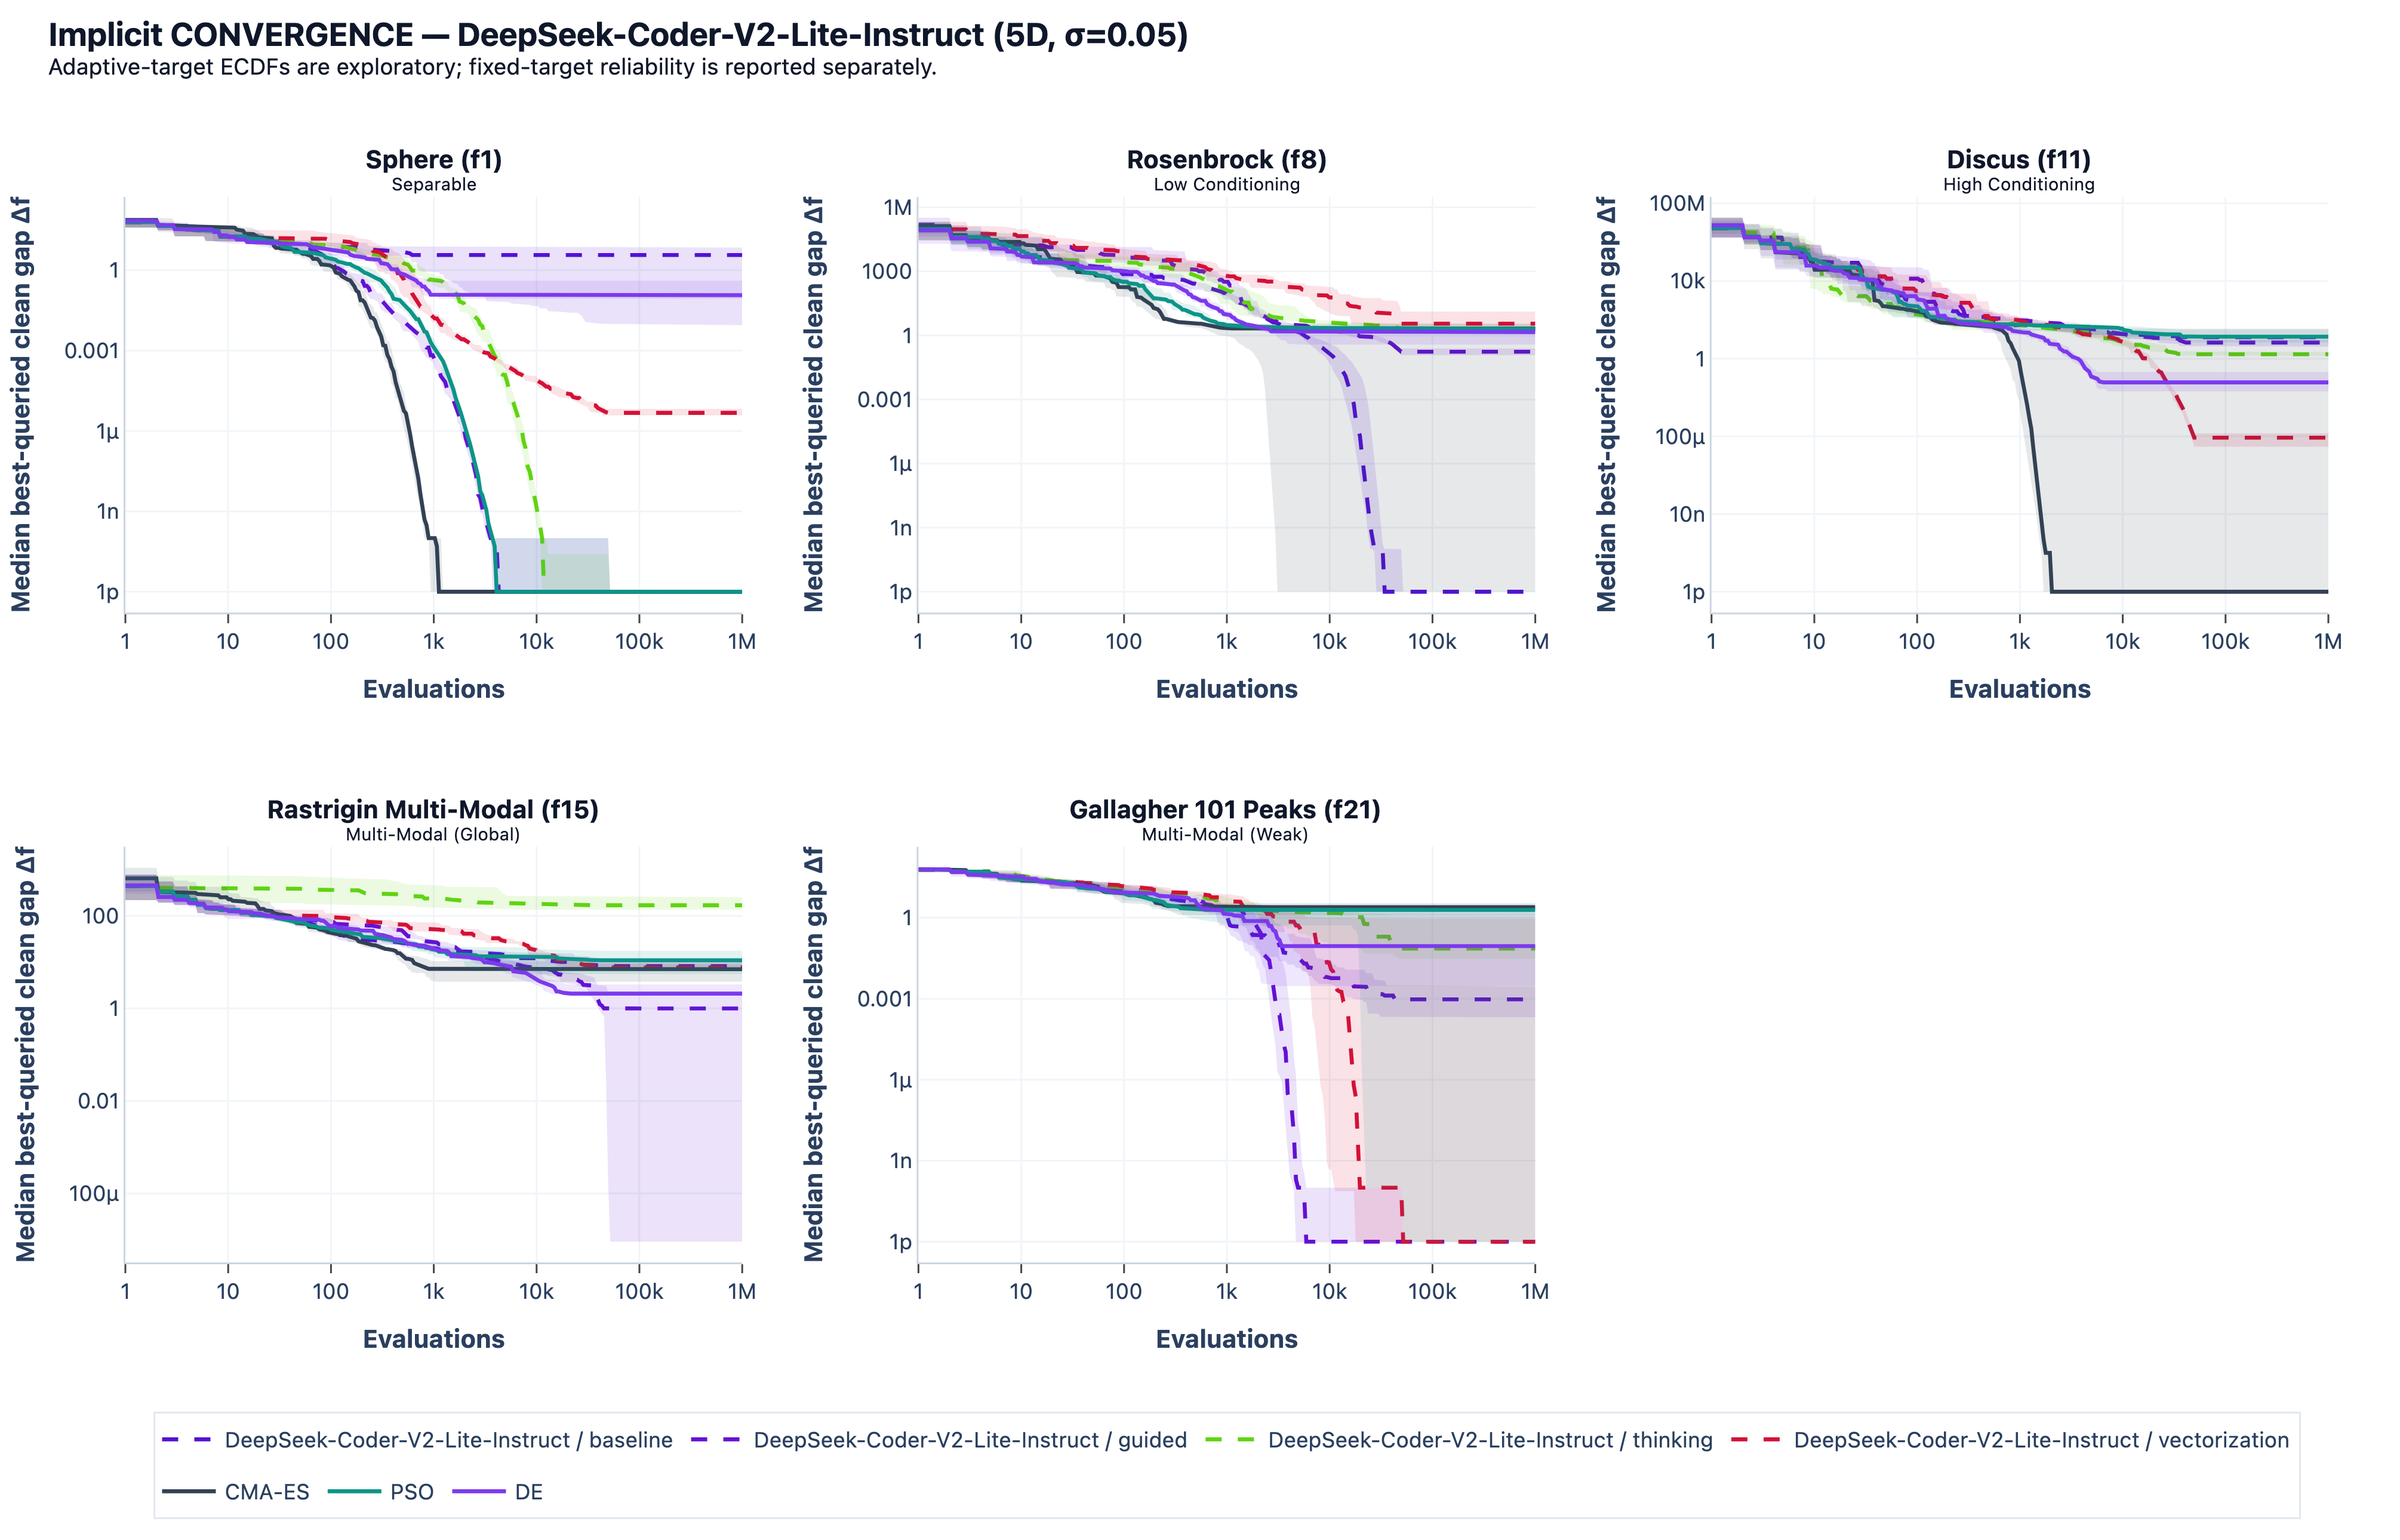
\includegraphics[width=\textwidth,height=0.32\textheight,keepaspectratio]{images/experiments/03_implicit/deepseek_coder_v2_lite_instruct_q4_k_m/5D/std_0.05/convergence_trajectories.png}
    \par\medskip
    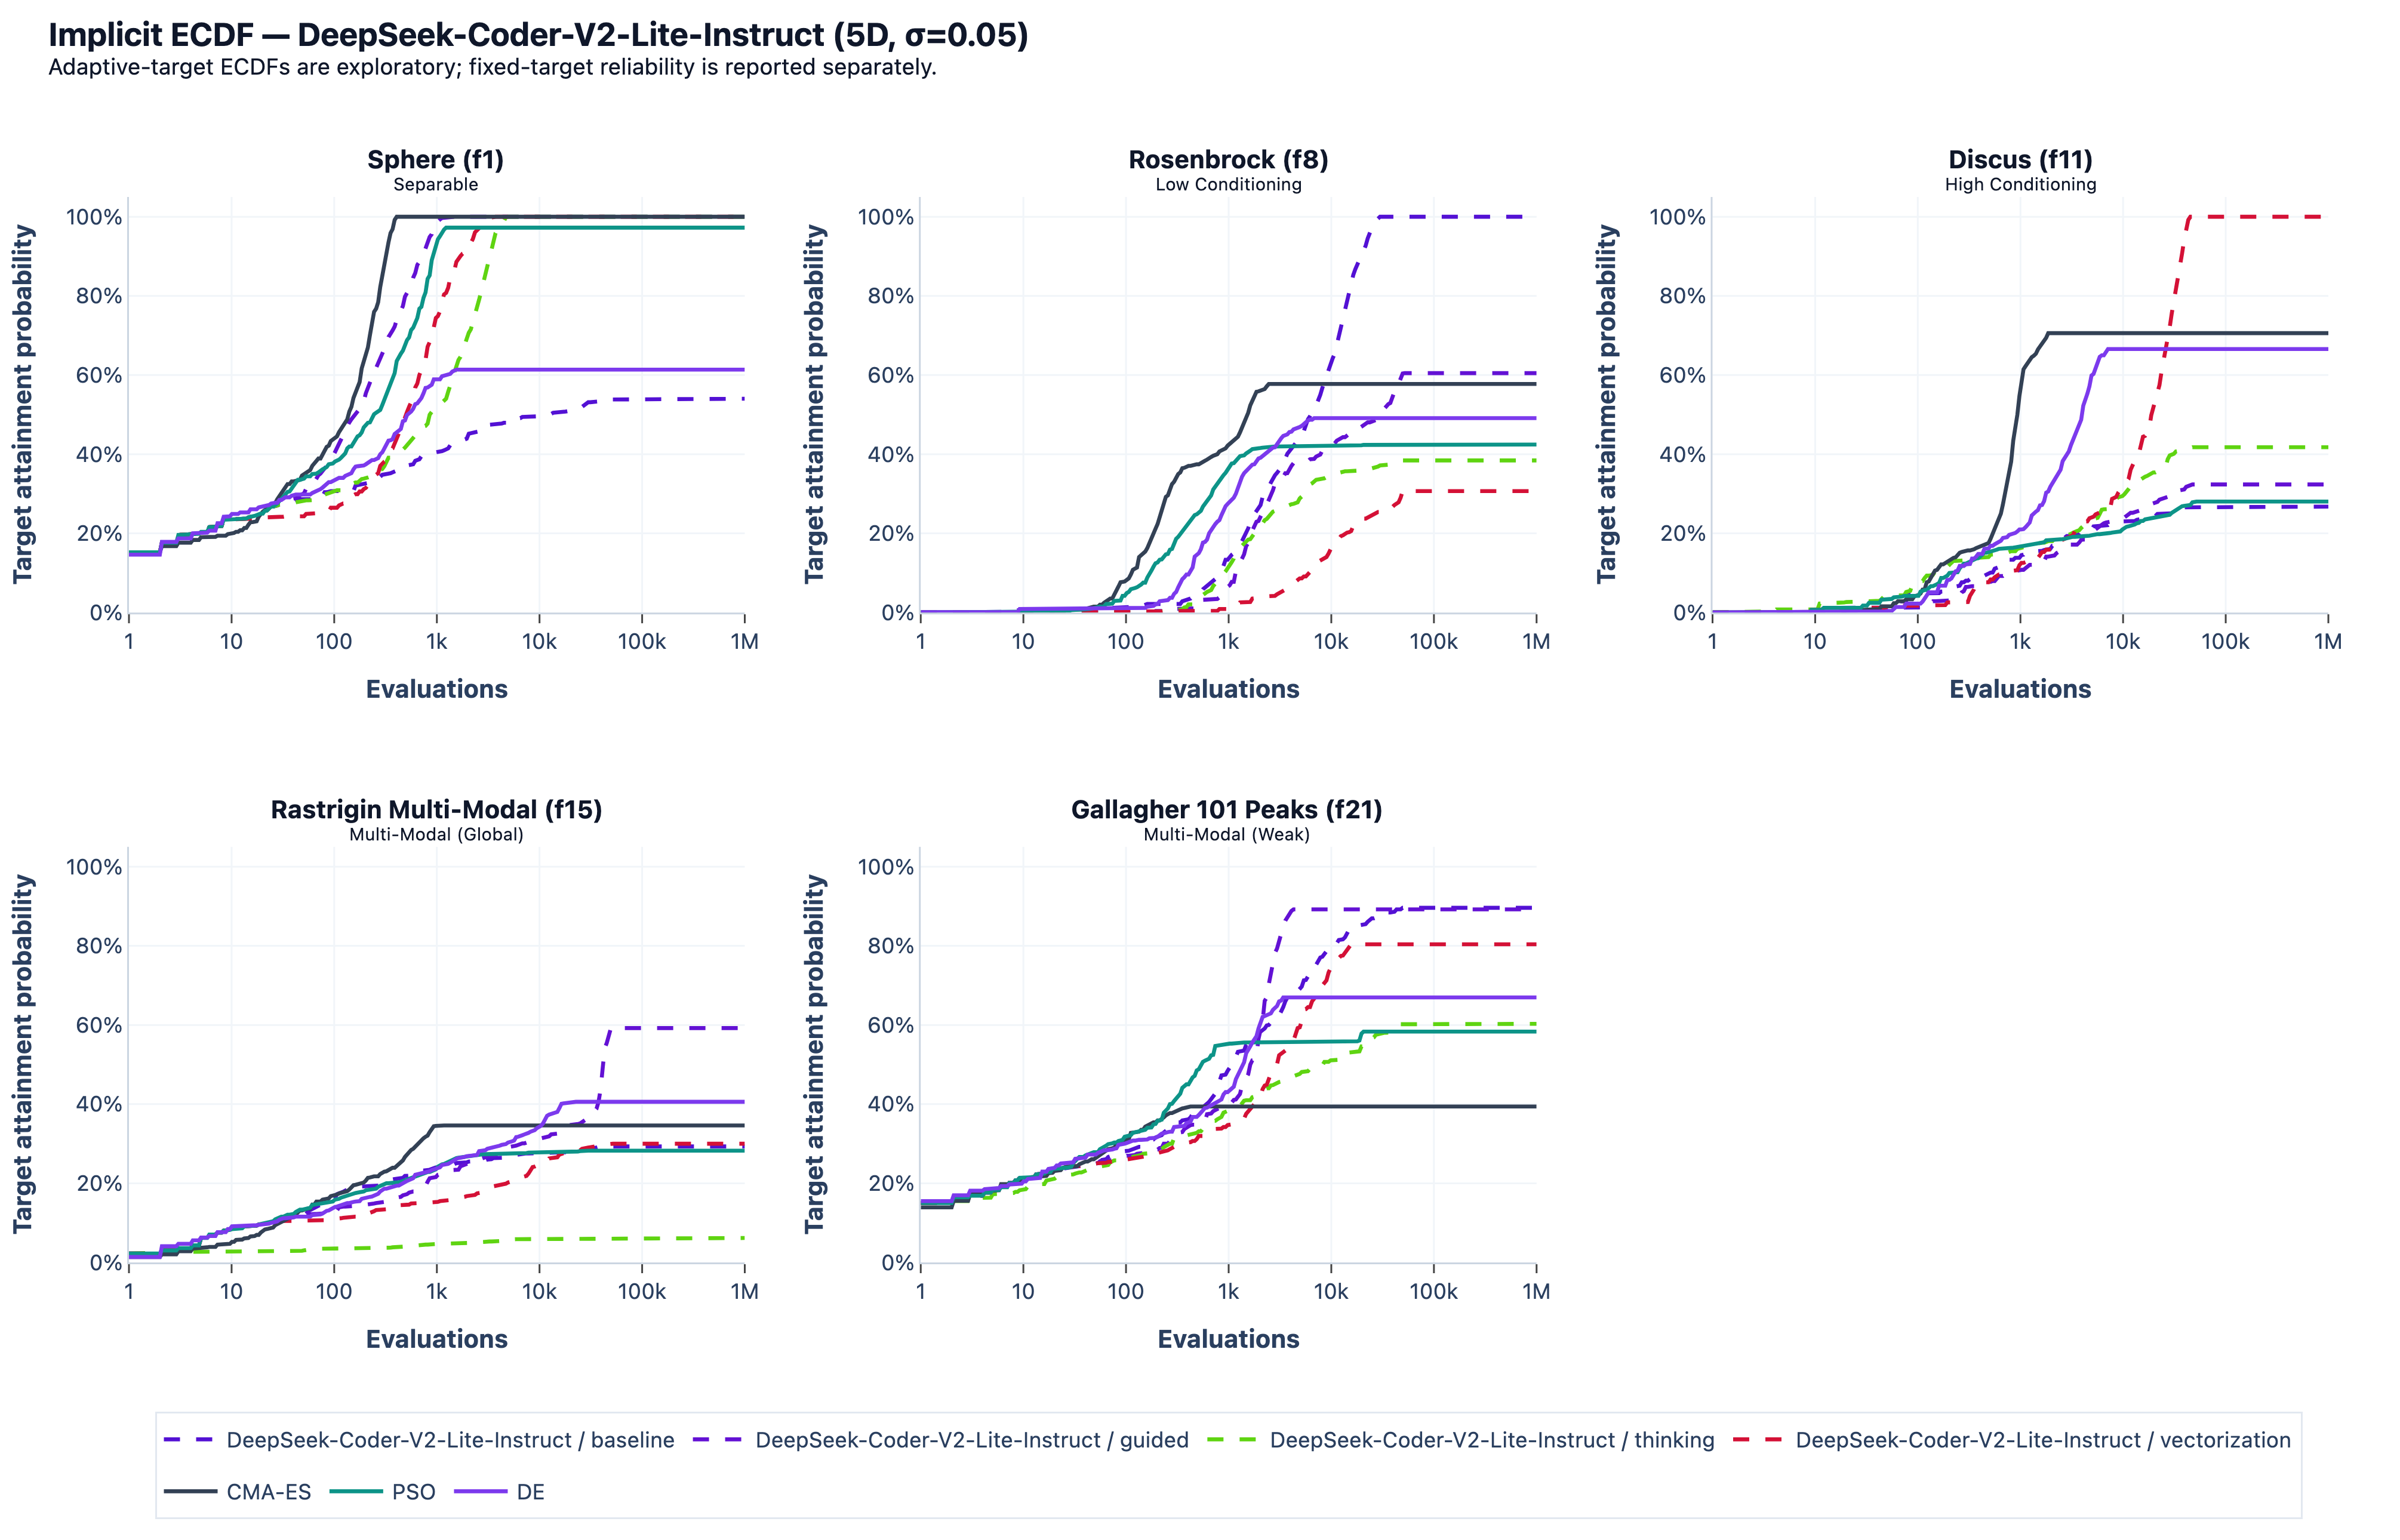
\includegraphics[width=\textwidth,height=0.32\textheight,keepaspectratio]{images/experiments/03_implicit/deepseek_coder_v2_lite_instruct_q4_k_m/5D/std_0.05/target_precision_ecdf.png}
    \caption{DeepSeek-Coder-V2-Lite-Instruct: Implicit, $D=5$,
    $\sigma=0.05$. Convergence (median and IQR) above;
    adaptive target-precision ECDF below. The objective-query allowance
    is 50,000.}
    \label{fig:appendix_03_implicit_deepseek_coder_v2_lite_instruct_q4_k_m_5_std_005}
\end{minipage}
\par\medskip

\par\smallskip\noindent
\begin{minipage}{\linewidth}
    \captionsetup{type=figure,aboveskip=4pt,belowskip=0pt}
    \centering
    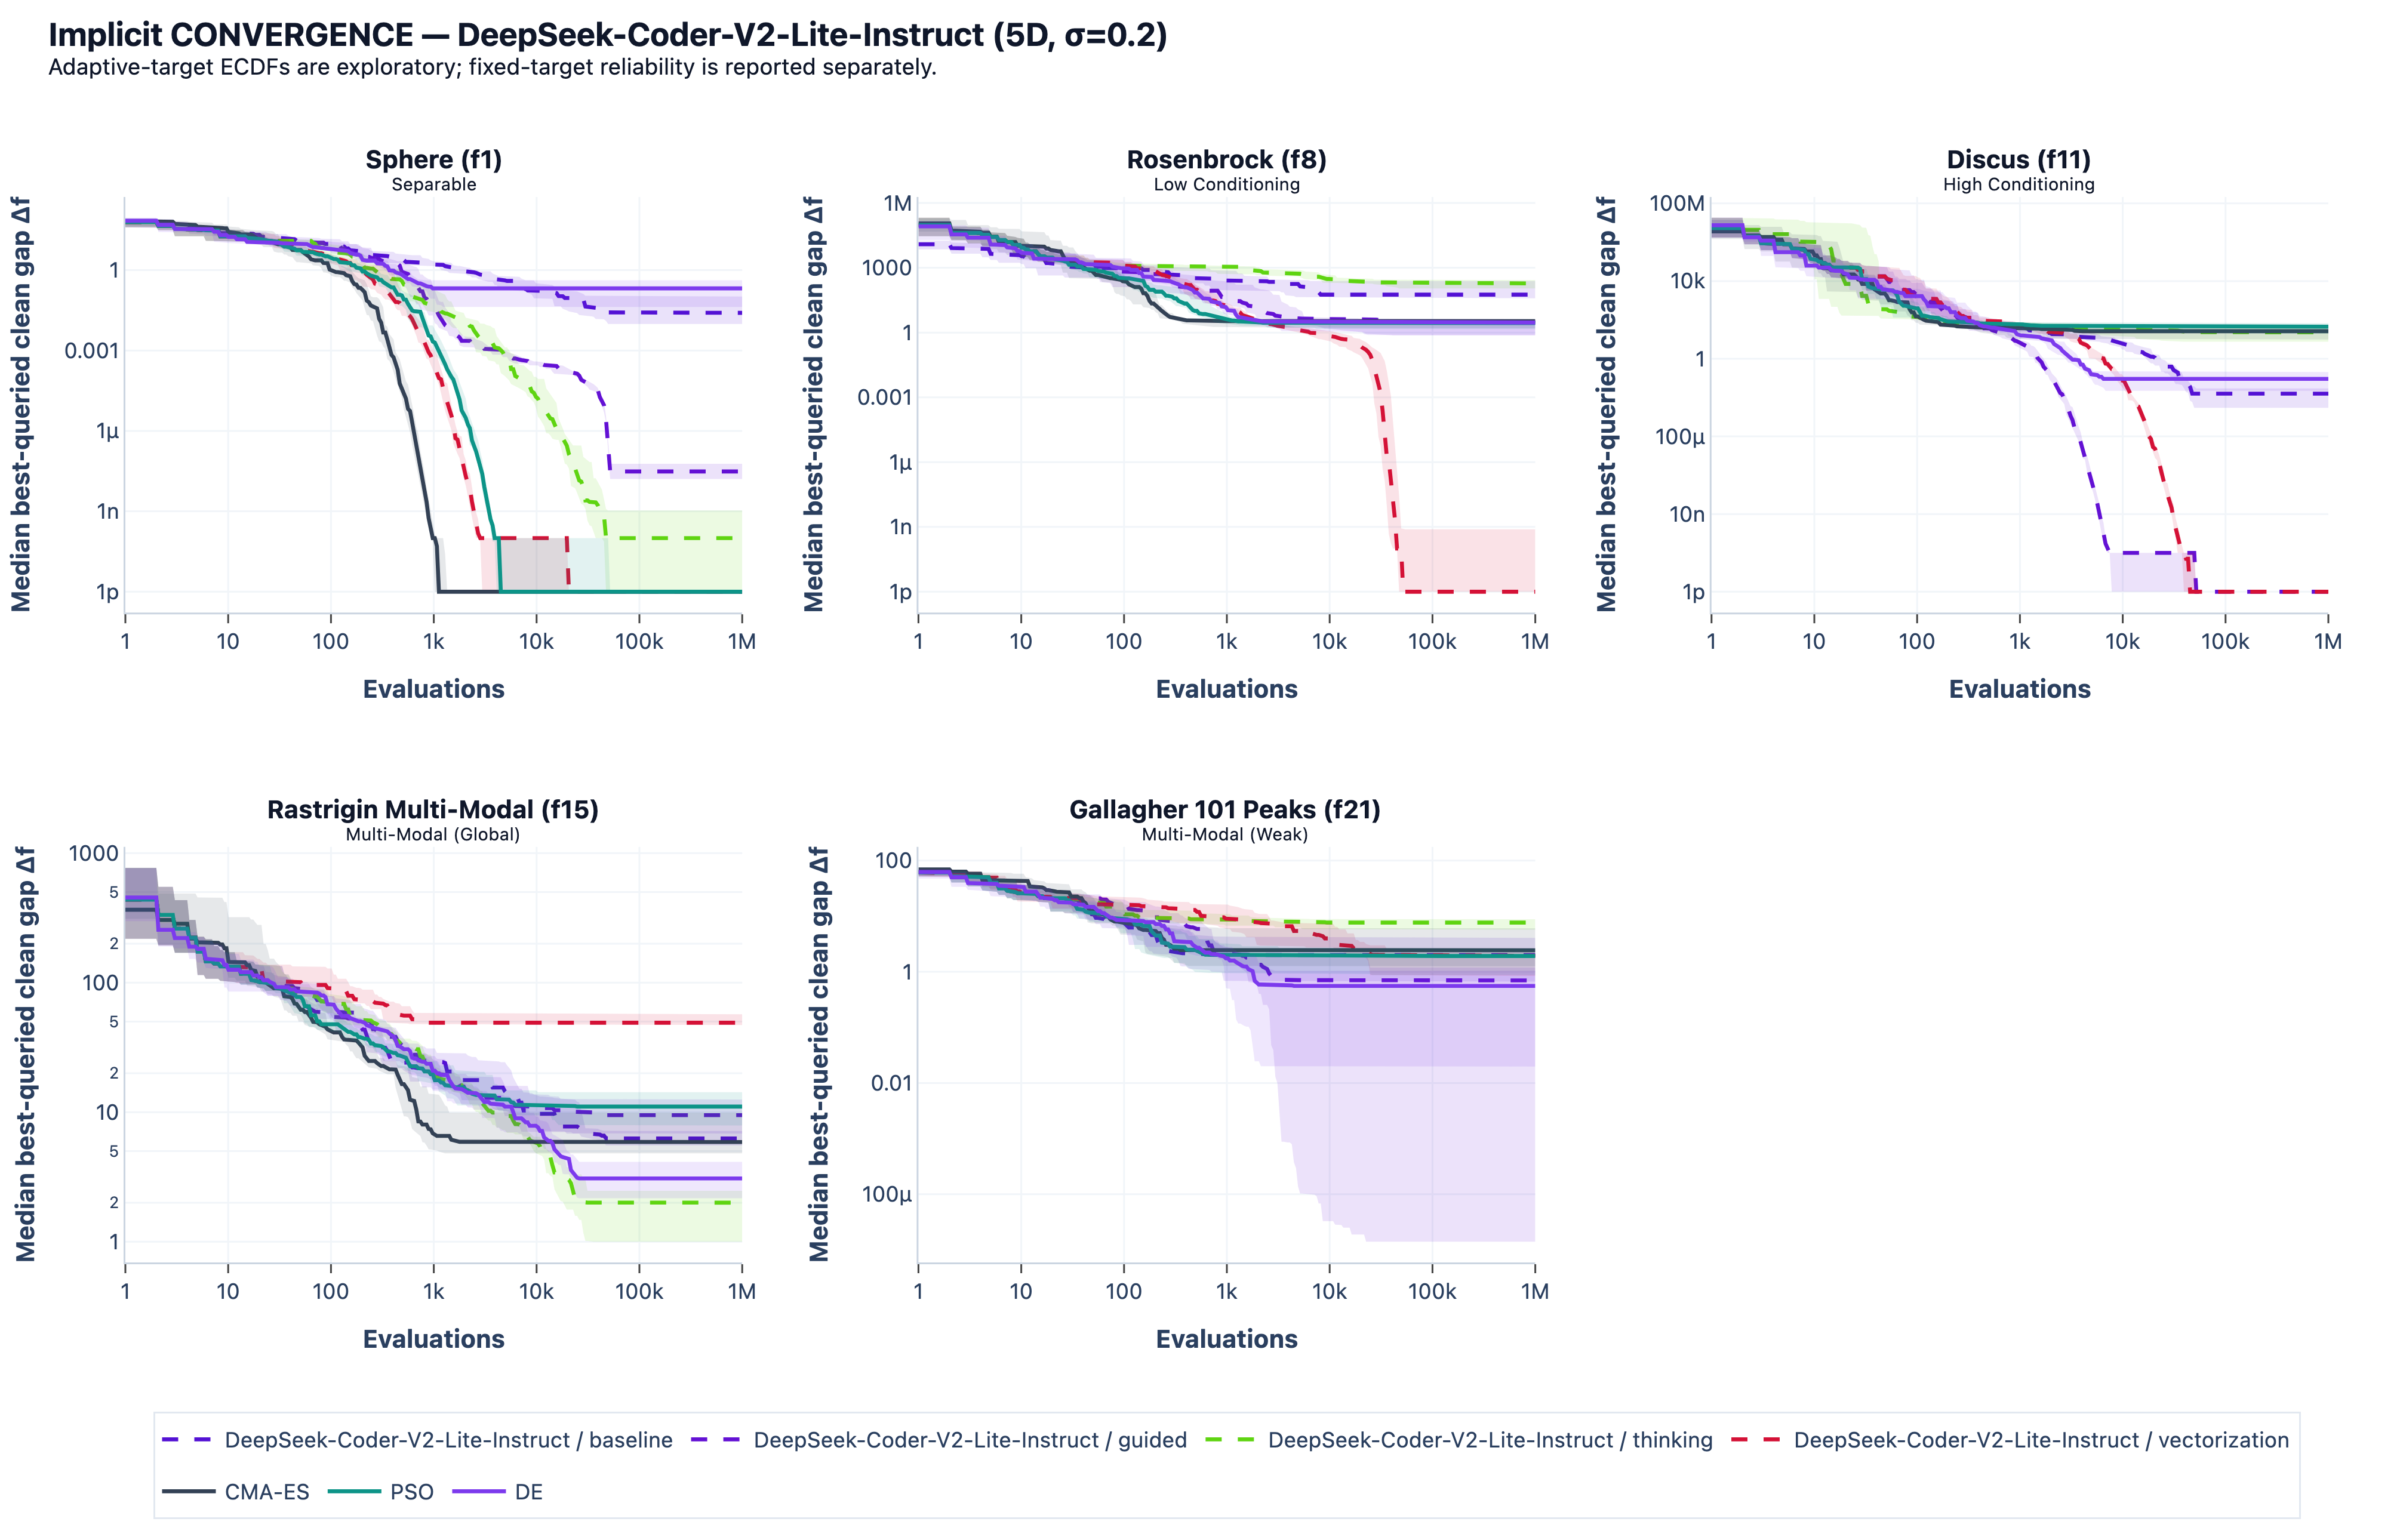
\includegraphics[width=\textwidth,height=0.32\textheight,keepaspectratio]{images/experiments/03_implicit/deepseek_coder_v2_lite_instruct_q4_k_m/5D/std_0.2/convergence_trajectories.png}
    \par\medskip
    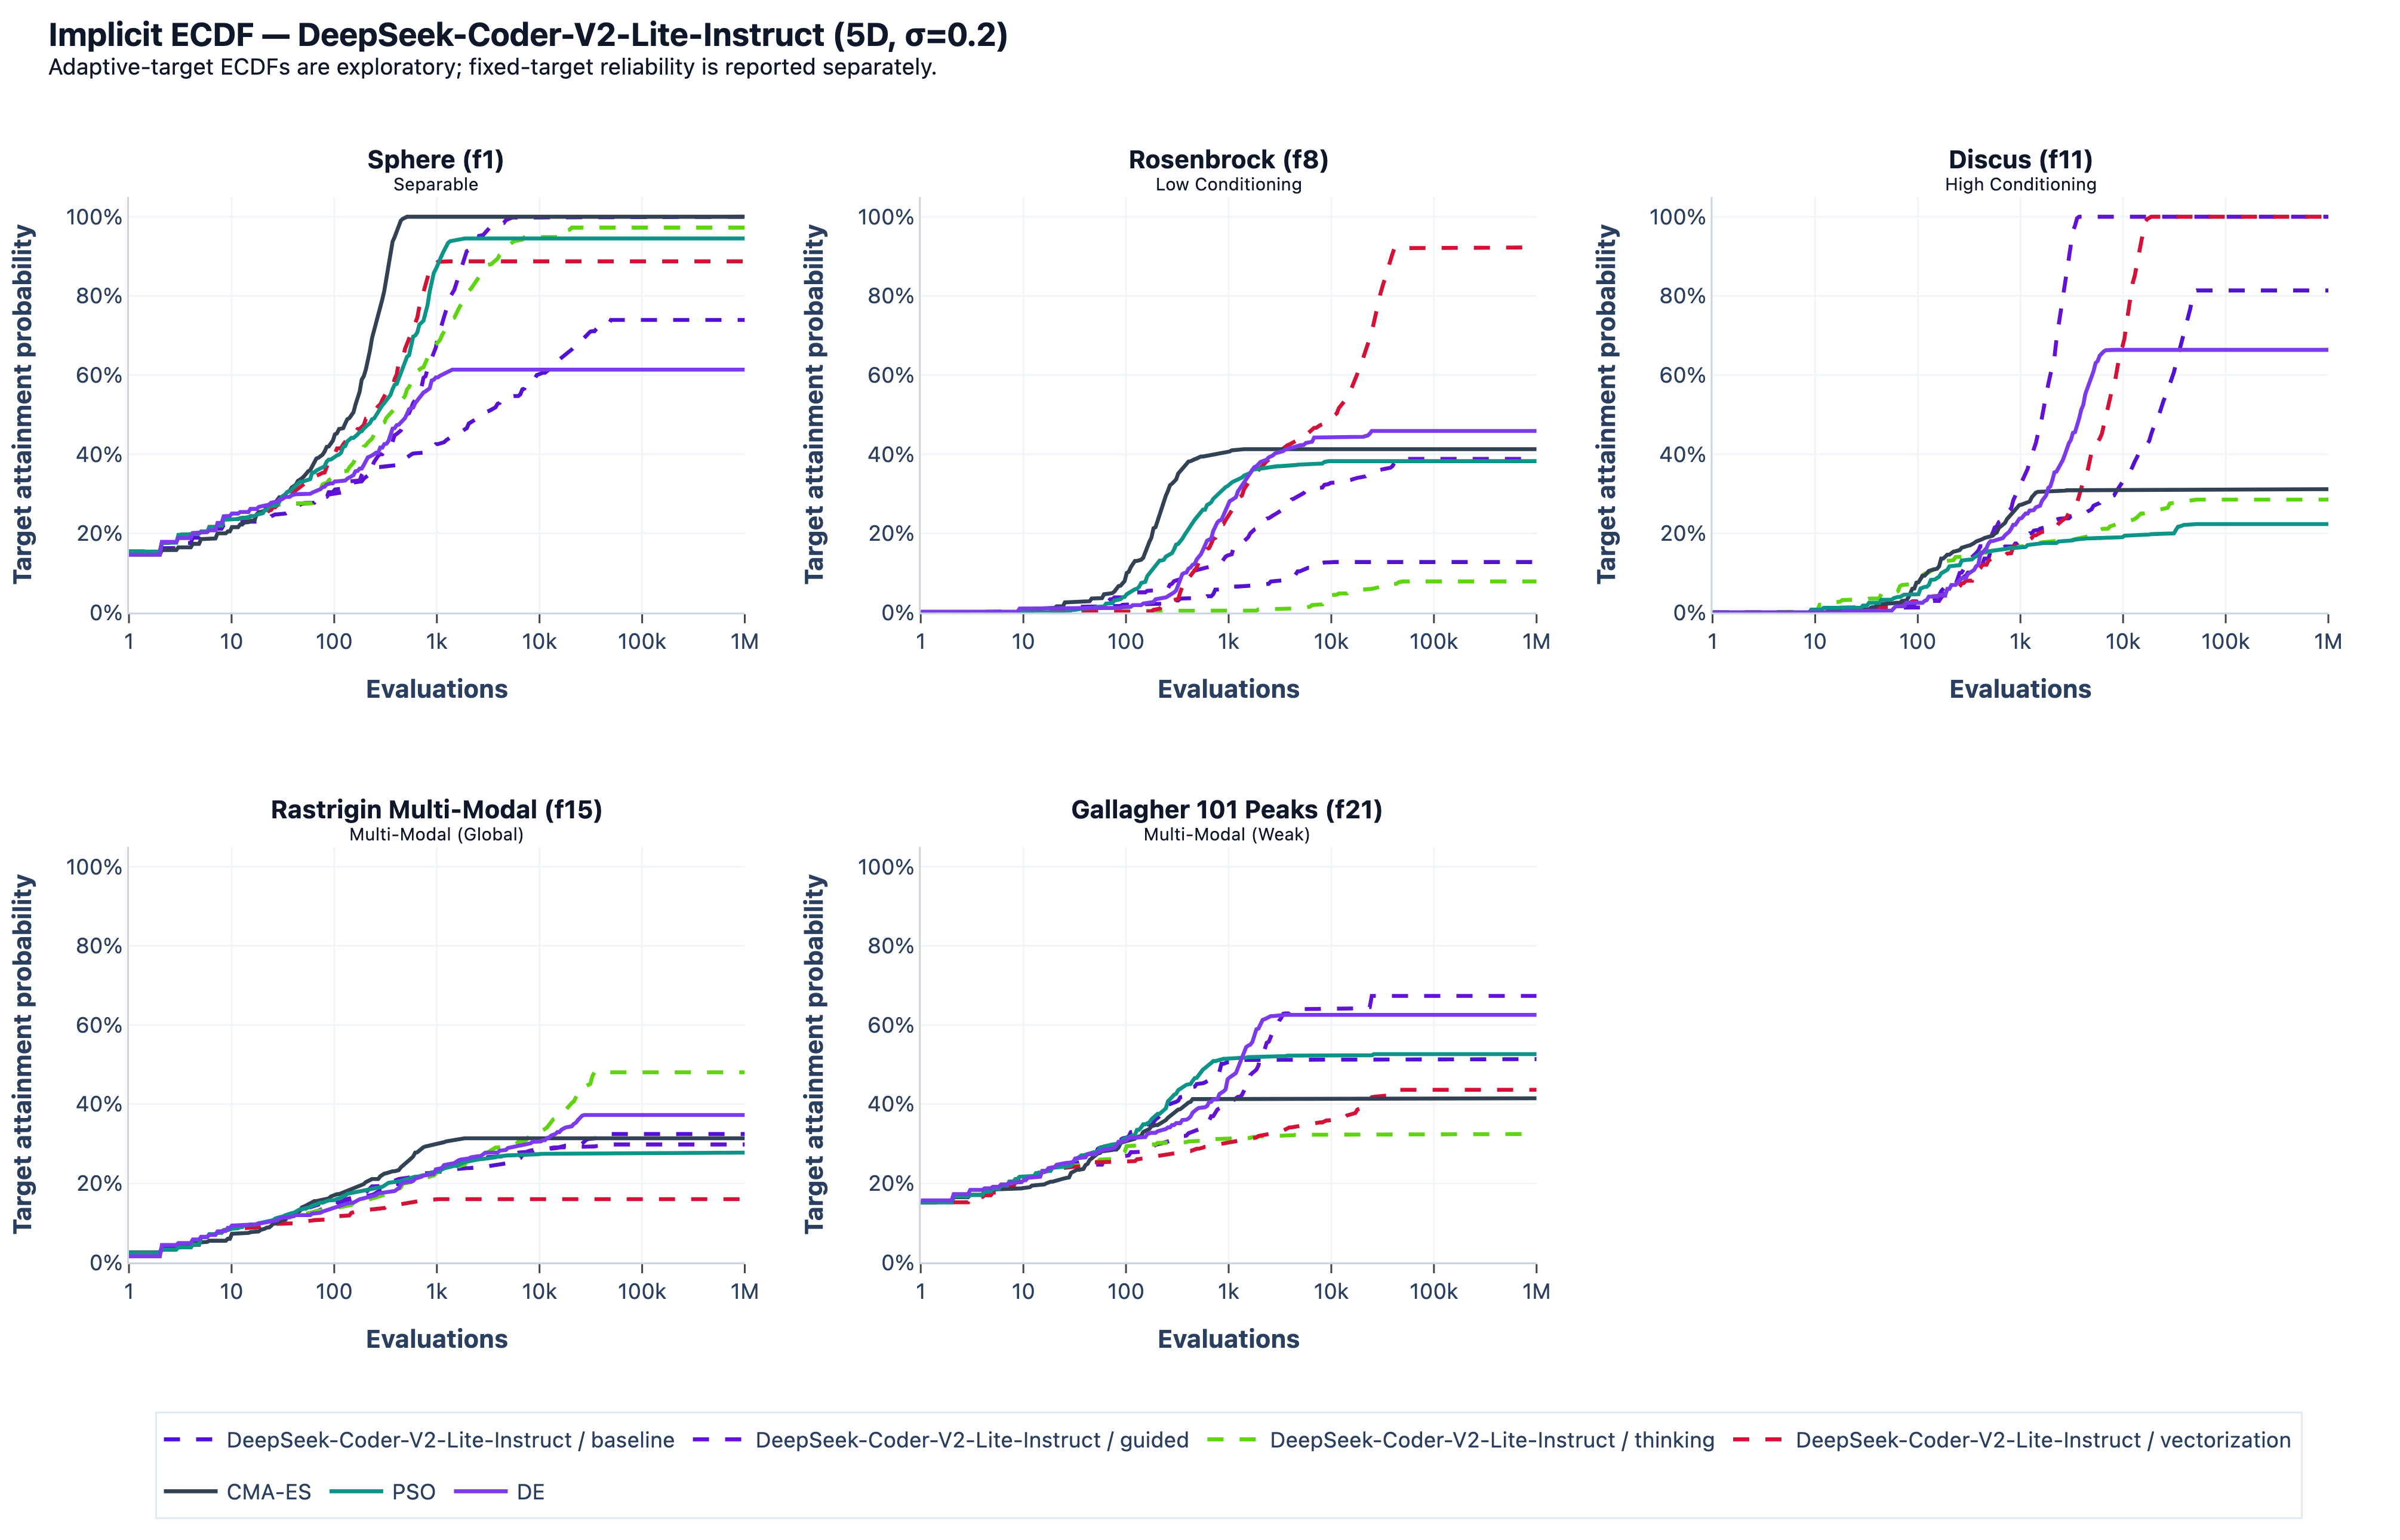
\includegraphics[width=\textwidth,height=0.32\textheight,keepaspectratio]{images/experiments/03_implicit/deepseek_coder_v2_lite_instruct_q4_k_m/5D/std_0.2/target_precision_ecdf.png}
    \caption{DeepSeek-Coder-V2-Lite-Instruct: Implicit, $D=5$,
    $\sigma=0.2$. Convergence (median and IQR) above;
    adaptive target-precision ECDF below. The objective-query allowance
    is 50,000.}
    \label{fig:appendix_03_implicit_deepseek_coder_v2_lite_instruct_q4_k_m_5_std_02}
\end{minipage}
\par\medskip


